\documentclass[11pt,]{article}
\usepackage[left=1in,top=1in,right=1in,bottom=1in]{geometry}
\newcommand*{\authorfont}{\fontfamily{phv}\selectfont}
\usepackage[]{mathpazo}


  \usepackage[T1]{fontenc}
  \usepackage[utf8]{inputenc}



\usepackage{abstract}
\renewcommand{\abstractname}{}    % clear the title
\renewcommand{\absnamepos}{empty} % originally center

\renewenvironment{abstract}
 {{%
    \setlength{\leftmargin}{0mm}
    \setlength{\rightmargin}{\leftmargin}%
  }%
  \relax}
 {\endlist}

\makeatletter
\def\@maketitle{%
  \newpage
%  \null
%  \vskip 2em%
%  \begin{center}%
  \let \footnote \thanks
    {\fontsize{18}{20}\selectfont\raggedright  \setlength{\parindent}{0pt} \@title \par}%
}
%\fi
\makeatother




\setcounter{secnumdepth}{3}

\usepackage{color}
\usepackage{fancyvrb}
\newcommand{\VerbBar}{|}
\newcommand{\VERB}{\Verb[commandchars=\\\{\}]}
\DefineVerbatimEnvironment{Highlighting}{Verbatim}{commandchars=\\\{\}}
% Add ',fontsize=\small' for more characters per line
\usepackage{framed}
\definecolor{shadecolor}{RGB}{248,248,248}
\newenvironment{Shaded}{\begin{snugshade}}{\end{snugshade}}
\newcommand{\KeywordTok}[1]{\textcolor[rgb]{0.13,0.29,0.53}{\textbf{#1}}}
\newcommand{\DataTypeTok}[1]{\textcolor[rgb]{0.13,0.29,0.53}{#1}}
\newcommand{\DecValTok}[1]{\textcolor[rgb]{0.00,0.00,0.81}{#1}}
\newcommand{\BaseNTok}[1]{\textcolor[rgb]{0.00,0.00,0.81}{#1}}
\newcommand{\FloatTok}[1]{\textcolor[rgb]{0.00,0.00,0.81}{#1}}
\newcommand{\ConstantTok}[1]{\textcolor[rgb]{0.00,0.00,0.00}{#1}}
\newcommand{\CharTok}[1]{\textcolor[rgb]{0.31,0.60,0.02}{#1}}
\newcommand{\SpecialCharTok}[1]{\textcolor[rgb]{0.00,0.00,0.00}{#1}}
\newcommand{\StringTok}[1]{\textcolor[rgb]{0.31,0.60,0.02}{#1}}
\newcommand{\VerbatimStringTok}[1]{\textcolor[rgb]{0.31,0.60,0.02}{#1}}
\newcommand{\SpecialStringTok}[1]{\textcolor[rgb]{0.31,0.60,0.02}{#1}}
\newcommand{\ImportTok}[1]{#1}
\newcommand{\CommentTok}[1]{\textcolor[rgb]{0.56,0.35,0.01}{\textit{#1}}}
\newcommand{\DocumentationTok}[1]{\textcolor[rgb]{0.56,0.35,0.01}{\textbf{\textit{#1}}}}
\newcommand{\AnnotationTok}[1]{\textcolor[rgb]{0.56,0.35,0.01}{\textbf{\textit{#1}}}}
\newcommand{\CommentVarTok}[1]{\textcolor[rgb]{0.56,0.35,0.01}{\textbf{\textit{#1}}}}
\newcommand{\OtherTok}[1]{\textcolor[rgb]{0.56,0.35,0.01}{#1}}
\newcommand{\FunctionTok}[1]{\textcolor[rgb]{0.00,0.00,0.00}{#1}}
\newcommand{\VariableTok}[1]{\textcolor[rgb]{0.00,0.00,0.00}{#1}}
\newcommand{\ControlFlowTok}[1]{\textcolor[rgb]{0.13,0.29,0.53}{\textbf{#1}}}
\newcommand{\OperatorTok}[1]{\textcolor[rgb]{0.81,0.36,0.00}{\textbf{#1}}}
\newcommand{\BuiltInTok}[1]{#1}
\newcommand{\ExtensionTok}[1]{#1}
\newcommand{\PreprocessorTok}[1]{\textcolor[rgb]{0.56,0.35,0.01}{\textit{#1}}}
\newcommand{\AttributeTok}[1]{\textcolor[rgb]{0.77,0.63,0.00}{#1}}
\newcommand{\RegionMarkerTok}[1]{#1}
\newcommand{\InformationTok}[1]{\textcolor[rgb]{0.56,0.35,0.01}{\textbf{\textit{#1}}}}
\newcommand{\WarningTok}[1]{\textcolor[rgb]{0.56,0.35,0.01}{\textbf{\textit{#1}}}}
\newcommand{\AlertTok}[1]{\textcolor[rgb]{0.94,0.16,0.16}{#1}}
\newcommand{\ErrorTok}[1]{\textcolor[rgb]{0.64,0.00,0.00}{\textbf{#1}}}
\newcommand{\NormalTok}[1]{#1}
\usepackage{longtable,booktabs}

\usepackage{graphicx,grffile}
\makeatletter
\def\maxwidth{\ifdim\Gin@nat@width>\linewidth\linewidth\else\Gin@nat@width\fi}
\def\maxheight{\ifdim\Gin@nat@height>\textheight\textheight\else\Gin@nat@height\fi}
\makeatother
% Scale images if necessary, so that they will not overflow the page
% margins by default, and it is still possible to overwrite the defaults
% using explicit options in \includegraphics[width, height, ...]{}
\setkeys{Gin}{width=\maxwidth,height=\maxheight,keepaspectratio}

\title{Ecología numérica de la familia Myrtaceae en la parcela permanente de
50-ha en Barro Colorado, lago Gatún, Panamá  }



\author{\Large Rosee Aurelina Féliz Méndez\vspace{0.05in} \newline\normalsize\emph{Estudiante, Universidad Autónoma de Santo Domingo (UASD)}  }


\date{}

\usepackage{titlesec}

\titleformat*{\section}{\normalsize\bfseries}
\titleformat*{\subsection}{\normalsize\itshape}
\titleformat*{\subsubsection}{\normalsize\itshape}
\titleformat*{\paragraph}{\normalsize\itshape}
\titleformat*{\subparagraph}{\normalsize\itshape}

\titlespacing{\section}
{0pt}{36pt}{0pt}
\titlespacing{\subsection}
{0pt}{36pt}{0pt}
\titlespacing{\subsubsection}
{0pt}{36pt}{0pt}





\newtheorem{hypothesis}{Hypothesis}
\usepackage{setspace}

\makeatletter
\@ifpackageloaded{hyperref}{}{%
\ifxetex
  \PassOptionsToPackage{hyphens}{url}\usepackage[setpagesize=false, % page size defined by xetex
              unicode=false, % unicode breaks when used with xetex
              xetex]{hyperref}
\else
  \PassOptionsToPackage{hyphens}{url}\usepackage[unicode=true]{hyperref}
\fi
}

\@ifpackageloaded{color}{
    \PassOptionsToPackage{usenames,dvipsnames}{color}
}{%
    \usepackage[usenames,dvipsnames]{color}
}
\makeatother
\hypersetup{breaklinks=true,
            bookmarks=true,
            pdfauthor={Rosee Aurelina Féliz Méndez (Estudiante, Universidad Autónoma de Santo Domingo (UASD))},
             pdfkeywords = {Myrtaceae, Myrteae, Ecología numérica, mirtáceas, parcela permanente de
50-ha, BCI},  
            pdftitle={Ecología numérica de la familia Myrtaceae en la parcela permanente de
50-ha en Barro Colorado, lago Gatún, Panamá},
            colorlinks=true,
            citecolor=blue,
            urlcolor=blue,
            linkcolor=magenta,
            pdfborder={0 0 0}}
\urlstyle{same}  % don't use monospace font for urls

% set default figure placement to htbp
\makeatletter
\def\fps@figure{htbp}
\makeatother

\usepackage{pdflscape} \newcommand{\blandscape}{\begin{landscape}}
\newcommand{\elandscape}{\end{landscape}} \usepackage{float}
\floatplacement{figure}{H}
\newcommand{\beginsupplement}{ \setcounter{table}{0} \renewcommand{\thetable}{S\arabic{table}} \setcounter{figure}{0} \renewcommand{\thefigure}{S\arabic{figure}} }


% add tightlist ----------
\providecommand{\tightlist}{%
\setlength{\itemsep}{0pt}\setlength{\parskip}{0pt}}

\begin{document}
	
% \pagenumbering{arabic}% resets `page` counter to 1 
%
% \maketitle

{% \usefont{T1}{pnc}{m}{n}
\setlength{\parindent}{0pt}
\thispagestyle{plain}
{\fontsize{18}{20}\selectfont\raggedright 
\maketitle  % title \par  

}

{
   \vskip 13.5pt\relax \normalsize\fontsize{11}{12} 
\textbf{\authorfont Rosee Aurelina Féliz Méndez} \hskip 15pt \emph{\small Estudiante, Universidad Autónoma de Santo Domingo (UASD)}   

}

}








\begin{abstract}

    \hbox{\vrule height .2pt width 39.14pc}

    \vskip 8.5pt % \small 

\noindent La ecología de comunidades nos ayuda a comprender la manera en que se
distribuyen los conjuntos de especies en la naturaleza, y los modos en
que estos agrupamientos están influenciados por su ambiente y las
interacciones intraespecíficas. En la isla de Barro Colorado, durante
los repetidos censos que se han realizado en la parcela permanente de
50-ha, se han reportado varias especies de mirtáceas, siendo su
representatividad relativamente importante en dicho enclave. Ninguna
investigación ha reportado ni analizado los patrones de la comunidad de
mirtáceas de la isla a la fecha. El objetivo general es conocer los
rasgos básicos de la estructura y composición de la comunidad de
mirtáceas en relación con factores ambientales de esta parcela. Se
hicieron estudios para medir el grado de asociación, agrupamiento,
diversidad y ecología espacial de esta familia con la ayuda de los
paquetes de R y con los datos del octavo censo de la parcela. Las
mirtáceas presentaron una riqueza de 7 especies y 4 géneros con una
abundancia de 5579 individuos pertencientes a la subtribu Myrteae. Las
especies del género \emph{Eugenia} presentaron altos grados de
asociación. El agrupamiento Ward de varianza mínima sugirió la partición
de 4 grupos que alcazaron el 100\% de la completitud de muestra. La
diversidad de mirtáceas posee una correlación positiva con \emph{Al, P,
Ca, Fe} y la geomorfología de pendiente media. Las especies
\emph{Chamguava schippii} y \emph{E. oerstediana} son las especies que
aportan a la diversidad beta y están estrechamente relacionadas con los
sitios (14 y 19) que aportan a la misma. El modelo de abundancia de
especies mostró que el 56\% de la comunidad presenta mayores valores de
equidad (log normal 10\% y null 46\%). \emph{C. schippii}, \emph{E.
oerstediana} y \emph{E. nesiotica} presentaron alta correlación
espacial, y otras como \emph{Myrcia gatunensis}, \emph{E. galalonensis}
y \emph{Psidium friedrichsthalianum} mostraron un patrón espacial
aleatorio. De los hallazgos, se infiere preliminarmente que \emph{M.
gatunensis} es endémica del lago Gatún, \emph{C. schippii} y \emph{E.
oerstediana} son basófilas y \emph{E. nesiotica} es acidófila. Este
estudio presenta nuevos conocimientos sobre las Myrteae, aunque solo se
queda en estadísticos debido a la falta de información que respalde o no
los hallazgos obtenidos, por lo que se necesitarán nuevos estudios de
las preferencias de variables ambientales y hábitats de las mirtáceas.


\vskip 8.5pt \noindent \emph{Keywords}: Myrtaceae, Myrteae, Ecología numérica, mirtáceas, parcela permanente de
50-ha, BCI \par

    \hbox{\vrule height .2pt width 39.14pc}



\end{abstract}


\vskip 6.5pt


\noindent  \section{Introducción}\label{introducciuxf3n}

Uno de los temas centrales en la ecología de comunidades es cómo
controlar la diversidad alfa, es decir, el número de especies que pueden
coexistir a escalas localizadas (e.g.~1 ha de una parcela). En las
plantas esta diversidad puede alcanzar niveles extraordinarios en los
bosques ecuatoriales. En el caso de los árboles de pequeños bosques
tropicales, ésta puede competir con la diversidad de árboles de los
bosques templados de todo un hemisferio. Otras formas de vida aumentan
la diversidad alfa en los bosques tropicales, especialmente las selvas
tropicales, donde los árboles representan sólo el 25\% de las especies
vegetales. Esta diversidad de las plantas es mayor en las selvas
tropicales ecuatoriales que en cualquier otro tipo de vegetación
(Wright, 2002).

La isla de Barro Colorado (BCI, por sus siglas en inglés) es un bosque
tropical, la isla se formó al término del canal de Panamá en 1914, desde
su creación se ha utilizado como centro de investigación debido a su
gran reserva natural. Se considera monumento natural protegido por el
gobierno de Panamá junto a las penínsulas Peña Blanca, Bohío, Buena
Vista, Frijoles y Gigante (Smithsonian Tropical Research Institute,
2010). La parcela permanente de 50 hectáreas se encuentra en el bosque
caducifolio húmedo tropical de la isla de Barro Colorado. Se estableció
en 1980, desde entonces se han realizado 8 censos (aprox. 1 cada 5
años), en los cuales se toman en cuenta árboles de tallos leñosos con un
diámetro a la altura del pecho (DAP) mayor a 10 mm, y como resultado en
cada censo, se han identificado, censado y mapeado más de 350,000
árboles individuales (Hubbell, Condit, \& Foster, 2021).

Las mirtáceas (Myrtaceae Juss) son una familia de plantas leñosas del
orden Myrtales, presentes en la parcela permanente de BCI. La mayoría de
las especies son árboles, también hay muchas que son arbustos o
subarbustos. Algunas especies producen flores y frutos, otras raíces
adventicias. Se distribuyen principalmente en zonas tropicales y
templadas, con poca representación en la región africana. La familia
cuenta con unos 142 géneros y más de 5.500 especies, incluyendo
\emph{Psiloxylon} y \emph{Heteropyxis}, también pueden ser citadas por
otros autores como familias monogenéricas Psiloxylaceae y
Heteropyxidaceae. Cabe destacar que la familia integra los árboles más
altos (110-140 m) del planeta (\emph{Eucalyptus}) y al género más
númeroso (1200‒1800 especies) que existe (\emph{Syzygium}), los
subarbustos rizomatosos de los géneros de la sabana (\emph{Psidium},
\emph{Campomanesia} y \emph{Eugenia}), el género \emph{Metrosideros} que
contiene especies arbóreas con muchas raíces adventicias, y otros
géneros son lianas trepadoras de raíces. También hay un mangle, el
monotípico \emph{Osbornia}, un pequeño árbol que carece de neumatóforos
(Wilson, 2010).

Las mirtaceas de BCI pertenecen a la subtribu Myrteae. Esta subtribu
posee especies que son ecológicamente importantes en muchos entornos
neotropicales debido a las bayas carnosas que comen aves y mamíferos, y
a las flores blancas generalistas que suministran polen y recursos a las
abejas. Debido a su importancia ecológica, los investigadores muestran
cada vez más interés en las Myrteae como grupo modelo para estudios
evolutivos, ecológicos y de conservación en biomas neotropicales. Cerca
del 70\% de la diversidad de especies descritas se encuentran en solo
dos géneros, \emph{Eugenia} y \emph{Myrcia}, y son dos de los géneros de
angiospermas más grandes, con 1000 y 700 especies, respectivamente.
Además, se ha demostrado sistemáticamente que estos dos géneros son
hermanos de linajes pobres en especies de la tribu, lo que aumenta la
disparidad de la diversidad existente entre clados estrechamente
relacionados. La mayor parte de la biodiversidad existente de Myrteae
está restringida al Neotrópico. En el continente americano, la mayor
diversidad de especies se encuentra en las selvas tropicales, la sabana
del centro, el este de Brasil, el escudo de Guayana y el Caribe; una
biodiversidad menor, pero aún significativa, se encuentra en la América
Central continental y en la cuenca del Amazonas de tierras bajas. La
diversidad de especies es relativamente baja en las zonas subtropicales
y templadas del sur de Sudamérica (Patagonia) y en los Andes de gran
altitud, pero con una importante variedad de géneros endémicos.

En BCI, durante los repetidos censos que se han realizado en la parcela
permanente de 50-ha desde 1981 (Hubbell et al., 2021), se han reportado
varias especies de mirtáceas, siendo su representatividad relativamente
importante en dicho enclave.

Mediante análisis exploratorios preliminares, se detectaron patrones
singulares de distribución espacial y de diversidad. Algunas especies
mostraron una distribución espacial concentrada (e.g. \emph{Chamguava
schippii}). Igualmente, varias especies mostraron preliminarmente
asociación con variables de suelo y geomorfólógicas. Ninguna
investigación ha reportado ni analizado estos patrones a la fecha. El
objetivo de este estudio es caracterizar la comunidad de mirtáceas de
BCI, con ayuda de técnicas de ecología numérica (e.g.~análisis de
asociación, agrupamiento, diversidad y ecología espacial en relación a
factores ambientales), utilizando como fuente los datos disponibles del
censo número de 8 de la parcela permanente de 50-ha.

\section{Metodología}\label{metodologuxeda}

\subsection{Preguntas de
investigación}\label{preguntas-de-investigaciuxf3n}

Medición de asociación:

-¿Se detectan especies asociadas dentro de las mirtaceas de BCI?

-¿Existe asociación entre variables ambientales/atributos? ¿Cuáles
variables?

Agrupamiento:

-Los cuadros (o quadrats) de 1 hectárea, ¿se organizan en grupos
discontinuos según la composición de las especies de mirtáceas?

-Si existe algún patrón, ¿es consistente con alguna variable
ambiental/atributo?

-¿Hay especies indicadoras o con preferencia por determinadas
condiciones ambientales/atributos?

Diversidad:

-Según los análisis de estimación de riqueza, ¿están representadas
suficientemente las mirtáceas en la parcela permanente de 50-ha de BCI?

-¿Existe asociación de la diversidad alpha con variables
ambientales/atributos? ¿Con cuáles?

-¿Existe contribución local o por alguna especie a la diversidad beta?

Ecología espacial:

-¿Alguna(s) especies de mirtáceas presenta(n) patrón aglomerado?
¿Cuál(es)? ¿Se asocia con alguna variable?

\subsection{Ámbito geográfico}\label{uxe1mbito-geogruxe1fico}

Los datos analizados fueron colectados en la parcela permanente de 50
hectáreas de la isla Barro Colorado (BCI en lo adelante). La parcela
está situada en la meseta central de la isla (latitud 9\(^\circ\)~9'N,
longitud 79\(^\circ\)~51'O), y fue establecida en 1980 por Stephen
Hubbell y Robin Foster. Posee 1,000 m de largo por 500 m de ancho, se
divide en 1250 cuadrantes de 20x20 m (ver figura
\ref{fig:mapa_cuadros_bci}). En la parcela, todos los tallos leñosos con
un diámetro a la altura de pecho (DAP) mayor o igual a 1 cm se
encuentran marcados, enumerados, mapeados e identicados hasta el nivel
de especie. Cada 5 años, esta parcela es censada para evaluar el
crecimiento, la mortalidad y para el reclutamiento de nuevas
generaciones de plantas. Como resultado de estos censos se han
registrado más de 300 especies de árboles, arbustos y palmas con el
próposito de conocer la historia de vida de las especies, interacciones
y dinámica de la comunidad (Pérez et al., 2005).

\begin{figure}
\centering
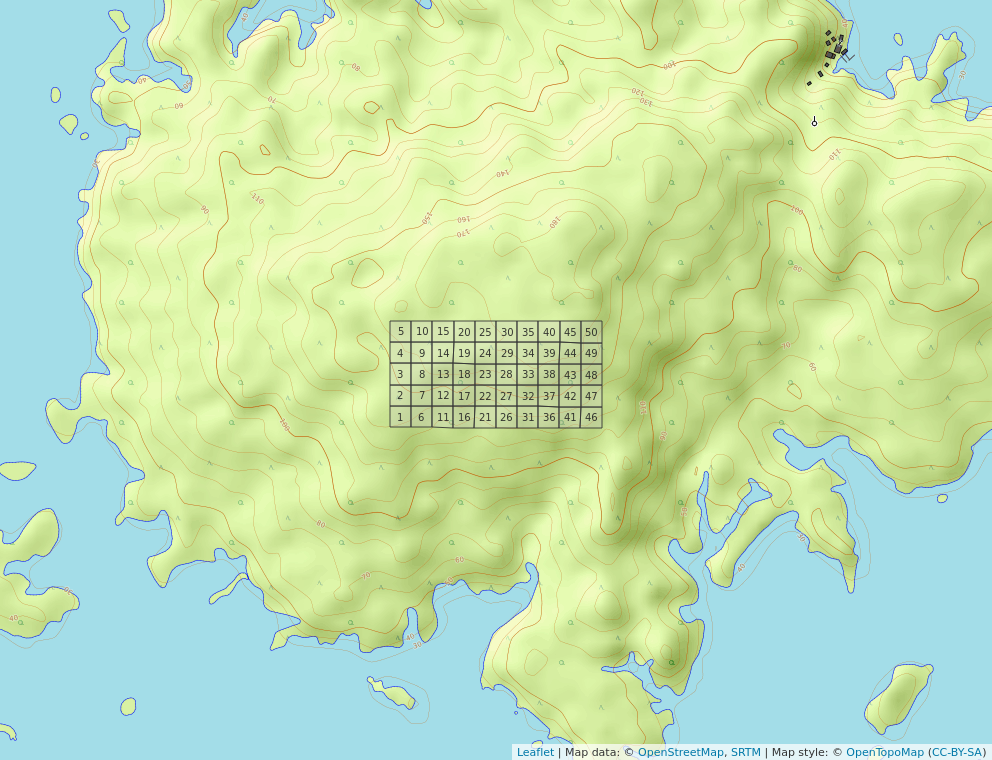
\includegraphics[width=0.50000\textwidth]{mapa_cuadros.png}
\caption{Parcela permanente de 50-ha dela isla Barro Colorado, lago
Gatún, Panamá \label{fig:mapa_cuadros_bci}}
\end{figure}

\subsection{Materiales y Métodos}\label{materiales-y-muxe9todos}

Se ha seleccionado el censo número 8 de esta reserva natural por ser el
más reciente y a esta reserva natural en particular debido a la gran
cantidad disponible de datos censales que a través de la Ecología
numérica nos permitirán conocer rasgos básicos de la estructura y
composición de la comunidad de plantas mirtáceas en relación con
factores ambientales.

Se exploraron los datos del censo número 8 disponibles en la página web
del censo (Hubbell et al., 2021), organizados en dos matrices: la matriz
de comunidad, la cual recopila la información referente a las especies
de la parcela permanente de 50-ha, y la matriz ambiental, que contiene
la información referente a las variables de suelo, geomorfológicas,
litológicas y de tipo de habitat. Los análisis, tablas, figuras y
gráficos se realizaron con los scripts de análisis de José R. Martínez
(Batlle, 2020) y con ayuda de los paquetes de R para análisis
estadísticos y ecológicos (R Core Team, 2019), cabe destacar los
paquetes \texttt{vegan} (Oksanen et al., 2019), \texttt{tidyverse}
(Wickham, 2017), \texttt{sf} (Pebesma, 2018), \texttt{mapview}
(Appelhans, Detsch, Reudenbach, \& Woellauer, 2019) y \texttt{leaflet}
(Cheng, Karambelkar, \& Xie, 2018) que fueron los más utilizados.

En los análisis de medición de asociación en modo Q, se utilizaron
varias distancias, como \emph{ji-cuadrado}, normalizada, Hellinger y
Jaccard. Las tres primeras son distancias euclideas, calculadas sobre
los datos transformados, apropiadas tanto para los datos cuantitativos
como para los datos de presencia-ausencia; y la última, la distancia de
Jaccard (\(D_J\)) se puede expresar como la proporción de especies no
compartidas. La distancia de Jaccard es el complemento a 1 de la
similaridad de Jaccard (\(S_J\)), es decir, \(D_J\) = 1- \(S_J\) , de
esta manera para obtener la similaridad, sólo hay que restarle el valor
de distancia a 1 (\(S_J\) = 1- \(D_J\)). Se puede usar para evaluar la
distancia entre especies, usando como fuente la matriz de comunidad
transpuesta convertida a binaria (presencia / ausencia) (Borcard, 2018).

Para el análisis de medición de asociación en modo R se utilizó el
coeficiente de correlación de Pearson, el cual tiene como objetivo medir
la fuerza o grado de asociación entre dos variables aleatorias
cuantitativas que poseen una distribución normal bivariada conjunta.
Alternativamente cuando este no cumple con los supuestos se utiliza
coeficiente de correlación no paramétrico de Spearman, que se define
como el coeficiente de correlación lineal entre los rangos Ri(x) y Ri(y)
(Restrepo \& González, 2007).

Se realizaron análisis de agrupamiento utilizando distintos métodos
(e.g.~UPGMA, \emph{Ward}) para explorar la estructura de la comunidad en
función de su composición. Para elegir entre métodos se utilizó la
correlación cofenética; se consideró al agrupamiento con la correlación
más alta como aquel que retiene la mayor parte de la información
contenida en la matriz de disimilitud; no obstante, esto no significa
necesariamente que este método sea el más adecuado para el objetivo del
investigador. Luego, para escoger una cantidad óptima de clústers para
cada agrupamiento se utilizó la anchura de la silueta, ésta es una
medida del grado de pertenencia de un objeto a su clúster, basada en la
disimilitud media entre este objeto y el clúster al que pertenece,
comparada con la misma medida del clúster más próximo (Borcard, 2018).

Los métodos aglomerativos utilizados para constatar y evaluar los grupos
que hacían sentido para las mirtáceas de este estudio son desarrollados
a continuación:

-El método aglomerativo por enlace simple (\emph{single}), conocido como
la clasificación por vecinos más cercanos, aglomera objetos en función
de sus disimilitudes más cortas entre pares: la fusión de un objeto con
un grupo en un nivel de disimilitud determinado sólo requiere que un
objeto de cada grupo que se aglomerare esté vinculado al otro en ese
nivel. En consecuencia, el dendrograma resultante de una aglomeración de
enlace simple suele mostrar encadenamiento de objetos. La lista de las
primeras conexiones que hacen a un objeto miembro de un clúster, o que
permite la fusión de dos clústeres, se denomina cadena de conexiones
primarias; esta cadena forma el árbol de expansión mínima (MST).

-El método aglomerativo por enlace completo (\emph{complete}), conocido
como la clasificación del vecino más lejano, permite que un objeto se
agrupe con otro grupo sólo en la disimilitud correspondiente a la del
par de objetos más distante; de esta manera con mayor motivo, todos los
miembros de los dos grupos están vinculados. Un grupo admite un nuevo
miembro sólo a una disimilitud correspondiente al objeto más lejano del
grupo. De ello se deduce que cuánto más grande es un grupo, más difícil
es aglomerarse con él. La vinculación completa resulta en muchos grupos
pequeños separados que se aglomeran a grandes distancias, por lo que
este método es interesante para buscar e identificar discontinuidades en
los datos.

-El método de grupos de pares no ponderados con media aritmética (UPGMA,
por sus siglas en inglés) es el más conocido de la familia métodos
aglomerativos por enlace promedio, éstos se basan en las disimilitudes
medias entre los objetos o en los centroides de los grupos. El método
UPGMA permite que un objeto se una a un grupo en la media de las
disimilitudes entre este objeto y todos los miembros del grupo. Cuando
dos grupos se unen, lo hacen a la media de las disimilitudes entre todos
los miembros de un grupo y todos los miembros del otro.

-El método de agrupación de varianza mínima de \emph{Ward} se basa en el
criterio del modelo lineal de mínimos cuadrados. Su objetivo es definir
los grupos de tal manera que la suma de cuadrados dentro del grupo (es
decir, el error cuadrático del ANOVA) se minimiza. La suma de errores al
cuadrado dentro del grupo puede calcularse como la suma de las
distancias al cuadrado entre los miembros de un grupo dividido por el
número de objetos (Borcard, 2018). Este método fue seleccionado porque
produce grupos con números de elementos más equilibrados, o que evita
los grupos de pocos elementos.

El remuestreo \emph{bootstrap} consiste en muestrear aleatoriamente
subconjuntos de los datos y calcular la agrupación en estos
subconjuntos. Luego de repetir este proceso un gran número de veces, se
cuenta la proporción de los resultados de clustering replicados en los
que aparece un cluster determinado. Esta proporción se denomina
probabilidad \emph{bootstrap} (BP) del cluster. Adicionalmente, se
aplicó el remuestreo \emph{bootstrap} multiescalar, utiliza muestras
\emph{bootstrap} de varios tamaños diferentes para estimar el valor p de
cada conglomerado. Esta mejora produce valores p ``aproximadamente
insesgados'' (AU) (Borcard, 2018).

Para evaluar homogeneidad de promedios de las variables ambientales
entre los grupos \emph{Ward} y las variables ambientales, se utilizaron
los análisis estadísticos ANOVA, que evalúa homogeneidad de medias, y
Kruskal-Wallis, que evalúa la homogeneidad de medianas; los cuales hacen
sentido para agrupamientos de 3 grupos o más (Batlle, 2020).

El análisis de especies indicadoras de los grupos \emph{Ward} se hizo
mediante el método del Valor Indicador (en lo adelante, IndVal), el cual
se calcula como el producto de la especificidad de una especie para el
grupo objetivo por su fidelidad al grupo. La especificidad se define por
la abundancia media de la especie dentro del grupo objetivo comparada
con su abundancia media en todos los grupos; la fidelidad es la
proporción de sitios del grupo en el que está presente la especie. Y el
análisis de especies con preferencia por hábitat se realizó mediante el
coeficiente de correlación biserial puntual que mide la relación entre
un vector que indica la presencia o abundancia de una especie en
diferentes lugares y un vector que describe a qué grupo predefinido
pertenece cada sitio (Borcard, 2018).

Para medir la diversidad alpha se utilizaron los índices de diversidad,
descritos a continuación:

-La equidad de Pielou (denominada también equidad de Shannon) equivale a
\(J=H_1/H_0\).

-Los tres primeros números de diversidad de Hill : \(N_0 =q\) (la
riqueza de especies), \(N_1 = e^H\) (número de especies abundantes), y
\(N_1 = 1/\)\(\lambda\) (inverso de Simpson).

-Los ratios de Hill: \(E_1 = N_1/N_0\) (versión de la equidad de
Shannon) y \(E_2 = N_2/N_0\) (versión de la equidad de Simpson)
(Borcard, 2018).

La equidad puede relacionarse con la forma de los modelos de abundancia
de especies, estos son funciones que describen la forma de los gráficos
de rango/abundancia en los que la abscisa clasifica las especies en
orden de abundancia decreciente y la ordenada representa las abundancias
transformadas en logaritmos. Los cuatro modelos principales son las
series geométricas, logarítmicas y lognormales, y el modelo de barra
rota. En este orden, la uniformidad aumenta de un modelo a otro en esta
secuencia (Borcard, 2018).

Para estimar la riqueza se utilizaron los modelos de enfoque asintótico:
a) paramétricos: Modelo homogéneo (estándar y MLE), este asume que todas
las especies tienen las mismas probabilidades de incidencia o detección;
y no paramétricos: Chao1, el cual utiliza las frecuencias de únicos y
duplicados para estimar el número de especies no detectadas, Chao1-bc
(forma corregida de sesgo para el estimador Chao1) e iChao1 (estimador
Chao1 mejorado); ICE (Estimador de cobertura basado en la incidencia) e
ICE-1 (ICE modificado para casos altamente heterogéneos); Jackknife de
primer orden, el cual utiliza la frecuencia de los ejemplares únicos
para estimar el número de especies no detectadas y jackknife de 2º
orden, que utiliza las frecuencias de los únicos y los duplicados para
estimar el número de especies no detectadas. Los cuales contienen un
intervalo de confianza del 95\%, para el cual se utiliza una
transformación logarítmica, de modo que el límite inferior del intervalo
resultante sea al menos el número de especies observadas (Chao et al.,
2014).

Basado en los supuestos de Whittaker, según los cuales la diversidad
beta es la variación espacial de la diversidad entre sitios dentro de un
área geográfica de interés. Existen diferentes ecuaciones para medir esa
variación. De la investigación sobre la diversidad beta existen dos
enfoques: (1) La diversidad beta puede interpretarse como una rotación,
es decir, el cambio direccional en la composición de la comunidad a lo
largo de un gradiente espacial, temporal o ambiental predefinido; y (2)
La diversidad beta también puede definirse como la variación de la
composición de la comunidad entre unidades de muestreo, sin referencia a
un gradiente explícito. Ambos conceptos entran en el ámbito de la
definición de Whittaker (Borcard, 2018).

Para obtener la contribuciones locales a la diversidad beta (LCBD), se
calcula primero la contribución del sitio i a la diversidad beta global
es la suma (SSi) de los valores centrados y al cuadrado del sitio (o
fila) i en la matriz S: 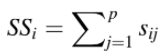
\includegraphics{beta_local.PNG}

y luego, la contribución relativa del sitio i a la diversidad beta, la
cual es denominada LCBD, es (Borcard, 2018):
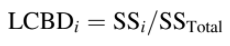
\includegraphics{beta_especies.png} donde
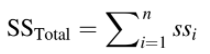
\includegraphics{beta_local2.PNG}

Para conocer las contribuciones de las especies a la diversidad beta
(SCBD), se calcula la contribución de la especie j a la diversidad beta
global es la suma (SSj) de los valores centrados y al cuadrado de la
especie (o columna) j en la matriz S:
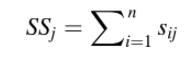
\includegraphics{beta_especies1.PNG}

y luego, la contribución relativa de la especie j a la diversidad beta,
que eso que se conoce como SCBD, es (Borcard, 2018):

\includegraphics{beta_especies2.PNG} donde
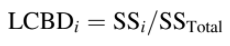
\includegraphics{beta_especies.png}

Para explorar patrones espaciales de las especies y las variables
ambientales, se utilizaron tanto el correlograma, como la prueba Mantel,
el índice de autocorrelación I de Moran y los mapas de indicadores
locales de autocorrelación espacial (en lo adelante Mapas LISA). Serán
descritos a continuación.

El correlograma es un gráfico de los valores de correlación espacial
frente a las clases de distancia, que combinado con pruebas
estadísticas, un correlograma permite evaluar rápidamente el tipo y el
alcance de la estructura de correlación espacial de una variable
(Borcard, 2018).

El Índice Global de Moran es un analisis estadístico que examina de
forma integral las variaciones de la autocorrelación espacial entre
valores vecinos más cercanos. Se clasifican de la siguiente manera,
cuando los valores tienden a agruparse se trata de una autocorrelación
espacial positiva, pero si se dispersan, es una autocorrelación
negativa, y si se distribuyen de forma aleatoria, se habla de que no hay
autocorrelación espacial entre los valores analizados(Bucheli, 2019). Se
construye de la siguiente manera (Borcard, 2018):
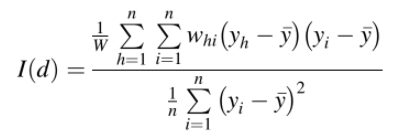
\includegraphics{moran1.PNG}

La correlación espacial en el ámbito multivariante puede evaluarse y
comprobarse mediante un correlograma de Mantel. Básicamente, se calcula
un estadístico de Mantel estandarizado rM (análogo al coeficiente r de
Pearson) entre una matriz de disimilitud entre sitios y una matriz donde
los pares de sitios que pertenecen a la misma clase de distancia reciben
el valor 0 y los demás pares, el valor 1. El proceso se repite para cada
clase de distancia. Cada valor de rM puede probarse mediante
permutaciones. La expectativa del estadístico de Mantel para la ausencia
de correlación espacial es rM \(1/4\) 0 (Borcard, 2018).

El Índice Local de Asociación Espacial (LISA) ayuda a identificar
patrones locales de asociación espacial, descomponiendo el Índice Moran
para evaluar la influencia de hábitats localizados en la estadística
global, esto se visualiza utilizando los Sistemas de Información
Geográfica. Este índice destaca las localizaciones con valores
estadísticos significativos en los indicadores, resaltando la presencia
de puntos calientes \emph{hot spots} o atípicos espaciales, dependiendo
de los datos estadísticos analizados. El resultado es la la generación
de un mapa que se denomina de agrupamiento o clúster, en este se
visualiza cada unidad espacial diferenciada de sus unidades vecinas
(Bucheli, 2019).

\section{Resultados}\label{resultados}

La familia Myrtaceae de la parcela permanente de 50-ha de BCI presentó
una abundancia de 5,579 individuos pertenecientes a 7 especies y 4
géneros de la subtribu Myrteae, de las cuales las más abundantes fueron
\emph{Eugenia galalonensis} y \emph{E. oerstediana}, representadas con
1,975 y 1,838 individuos cada una, y las especies más raras fueron
\emph{Psidium friedrichsthalianums} y \emph{Myrcia gatunensis}, con 58 y
56 individuos respectivamente (ver figura \ref{tab:abun_sp}).

\begin{longtable}[]{@{}lr@{}}
\caption{\label{tab:abun_sp}Abundancia por especie de la familia
Myrtaceae}\tabularnewline
\toprule
Latin & n\tabularnewline
\midrule
\endfirsthead
\toprule
Latin & n\tabularnewline
\midrule
\endhead
Eugenia galalonensis & 1975\tabularnewline
Eugenia oerstediana & 1838\tabularnewline
Eugenia coloradoensis & 609\tabularnewline
Chamguava schippii & 541\tabularnewline
Eugenia nesiotica & 502\tabularnewline
Psidium friedrichsthalianum & 58\tabularnewline
Myrcia gatunensis & 56\tabularnewline
\bottomrule
\end{longtable}

\begin{figure}
\centering
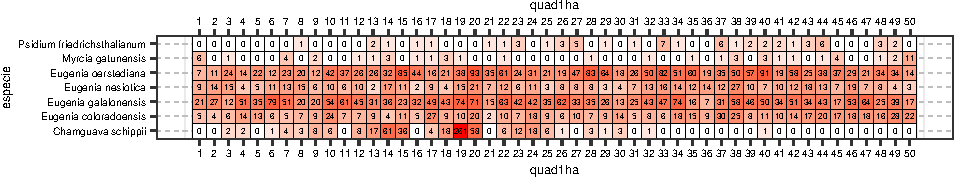
\includegraphics{manuscrito_files/figure-latex/unnamed-chunk-3-1.pdf}
\caption{\label{fig:abun_sp_q}Abundancia de especies por quadrat}
\end{figure}

Para los análisis de medición de asociación, la distancia de
\emph{ji}-cuadradado y la distancia de Jacard resultaron pequeñas entre
especies del genéro \emph{Eugenia} (\emph{E. oerstediana}, \emph{E.
galalonensis}, \emph{E. nesiotica} y \emph{E. coloradoensis}), lo cual
sugiere un patrón de dependencia, debido a que tienen altos grados de
asociación; y las especies \emph{P. friedrichsthalianum}, \emph{M.
gatunensis} y \emph{Chamguava schippii} presentan un posible patrón
independiente, no parecen asociarse con otras (ver figura
\ref{fig:matriz_Jacard}). La riqueza de la familia presentó asociación
estadística, a través del índice de Spearman, en términos positivos con
\emph{Al}, \emph{P} y en términos negativos con \emph{Ca}; y la
abundancia de mi familia presentó asociación estadística, a través del
índice de Spearman y el índice de Pearson, en términos positivos con
\emph{Al} y elevación media, y en términos negativos con \emph{Ca},
heterogeneidad ambiental y geomorfología de vaguada (ver figuras
\ref{fig:matriz_spearman} y \ref{fig:matriz_pearson}).

\begin{figure}
\centering
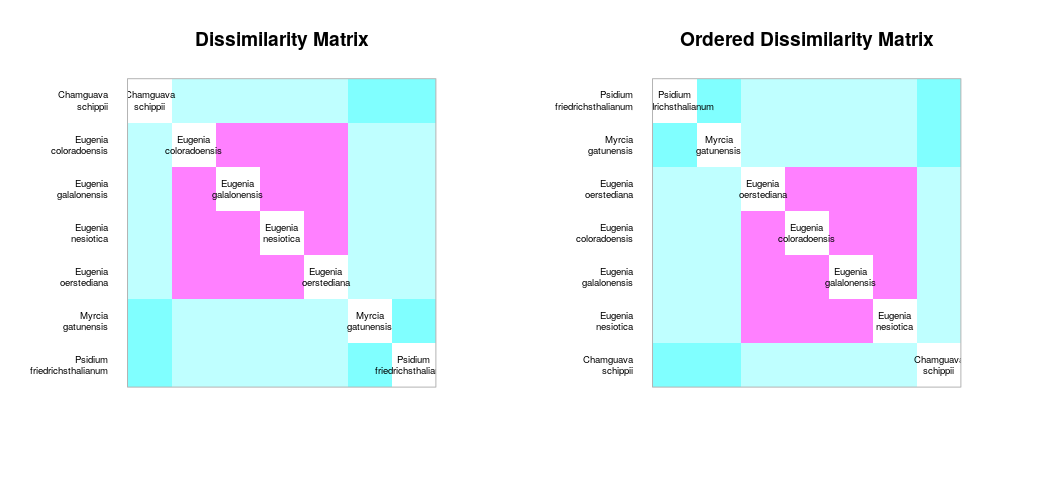
\includegraphics{Disimilaridad_.png}
\caption{Matriz de disimilaridad de Jacard \label{fig:matriz_Jacard}}
\end{figure}

Para los análisis de agrupamiento (\emph{cluster analysis}), se utilizó
el método de agrupamiento \emph{Ward} de varianza mínima conjuntamente
con el mapa de calor (ver figuras \ref{fig:mapadecalor_ward} y
\ref{fig:ward_fraccionado}), los cuales mostraron que las mirtáceas de
la parcela permanente de 50-ha de BCI se distribuyen en 4 grupos, de 20,
13, 2 y 15 sitios, respectivamente (ver figura \ref{fig:mapa_ward}). Los
métodos de agrupamiento aglomerativos por enlace simple, por enlace
completo y por enlace promedio (grupos de pares no ponderados con media
aritmética, UPGMA por sus siglas en inglés) destacaron la singularidad
de este grupo formado por dos sitios (14 y 19)(ver figura
\ref{fig:metodosdeagrupamiento}). Además, el remuestreo de
\emph{bootstrap} multiescalar respaldó este grupo con un probabilidad de
\emph{bootstrap} (BP) de 76 \% y probabilidad de valores aproximadamente
insesgados (AU) de 99 \%, de que sea un grupo real (ver figura
\ref {fig:*bootstrap*_multiescalar}). Las mirtáceas presentaron
asociación estadística, según las pruebas ANOVA y Kruskal-Wallis para
una significancia por debajo de 0.05 y el diagrama de cajas, con
variables de suelo: \emph{pH, Cu, Zn, Ca, Mg, N, Al} y \emph{K}; y
atributos del terreno: pendiente\_media, orientacion\_media,
elevación\_media, geomorf\_espolon/gajo\_pct (ver figuras
\ref{fig:ward_con_variables} y \ref{fig:anova_kruskalwallis_ward}).

\begin{figure}
\centering
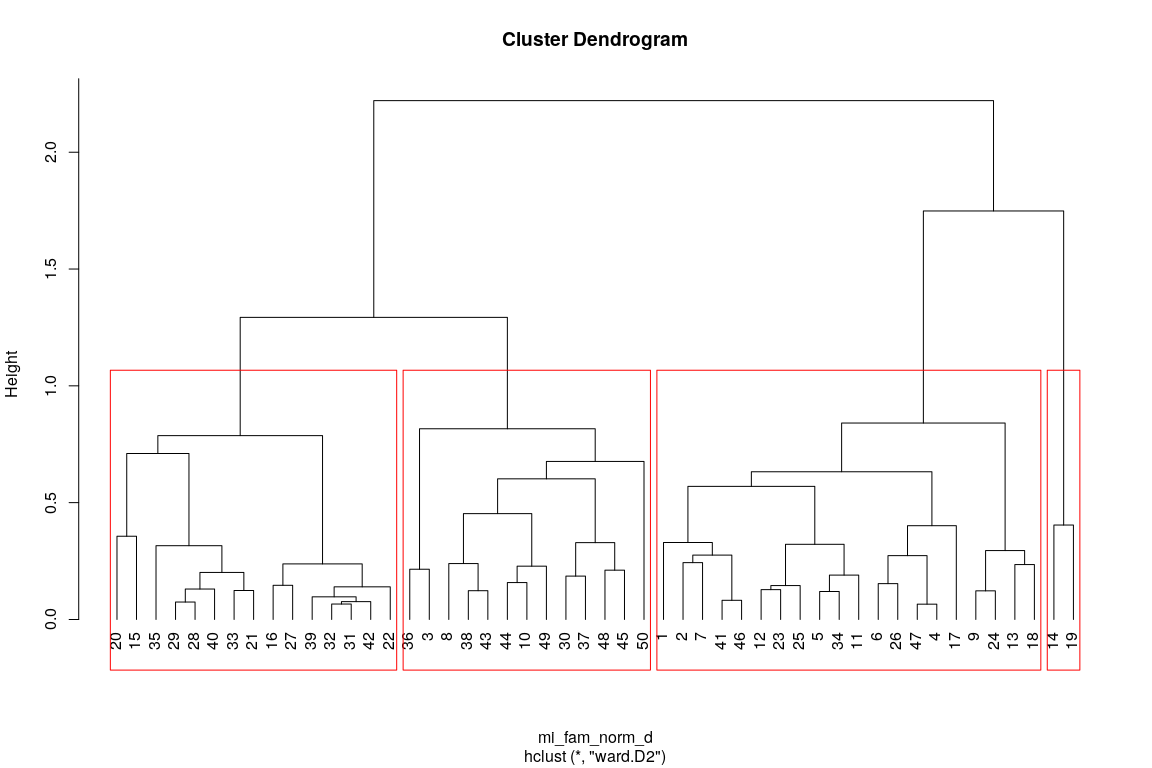
\includegraphics[width=0.50000\textwidth]{ward_fracionado.png}
\caption{Agrupamiento por el método \emph{Ward} de varianza mínima de
las mirtáceas \label{fig:ward_fraccionado}}
\end{figure}

Para este agrupamiento, las especies asociadas como indicadoras,
mediante IndVal para una significancia menor de 0.05, fueron \emph{C.
schippii} para el grupo 3, \emph{E. coloradoensis} para el conjunto de
grupos 1+2 y \emph{E. oerstediana} para el conjunto de grupos 3+4 (ver
figura \ref{fig:indval_analisis}); y las especies con preferencia por
hábitat, mediante el coeficiente de correlación biserial puntual para
una significancia menor de 0.05, fueron \emph{E. coloradoensis} con
preferencia por el grupo 2, \emph{C. schippii} por el grupo 3 y \emph{E.
oerstediana} por el grupo 4 (ver figura \ref{fig:rg_analisis}).

\begin{figure}
\centering
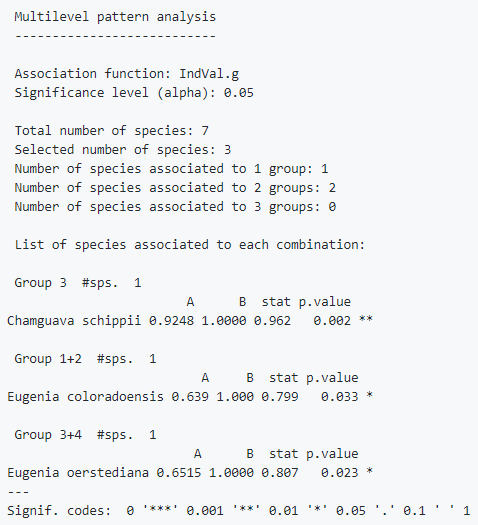
\includegraphics{inval_analisis.png}
\caption{Análisis de especies indicadoras de los grupos \emph{Ward},
mediante el método del Valor Indicador (IndVal)
\label{fig:indval_analisis}}
\end{figure}

\begin{figure}
\centering
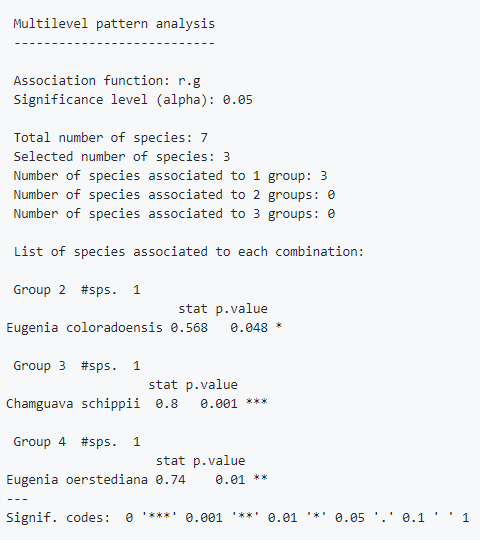
\includegraphics{rg_analisis.png}
\caption{Análisis de especies con preferencia por hábitats en los grupos
\emph{Ward}, mediante el coeficiente de correlación biserial puntual
\label{fig:rg_analisis}}
\end{figure}

Para los análisis de diversidad alpha las mirtáceas de este ámbito
geográfico presentaron, a través de la riqueza (\(N_0\)), \(E_2\) y
\(N_2\) de Hill, una correlación positiva importante con \emph{Al, P, Ca
y Fe}. Además, la diversidad de la familia, a través de la equidad de
Pielou (J) y los ratios de Hill (\(E_1\) y \(E_2\)) y \(N_2\), mostró
una correlación positiva notable con la presencia de la geomorfología de
pendiente media (ver figura \ref{fig:pearson_div}).

El modelo de abundancia de especies mostró que el 56\% de los quadrats
presenta mayores valores de equidad (log normal 10\% y null 46\%) (ver
figura \ref{fig:modelo_abundancia}). También se utilizaron los modelos
de estimación de riqueza (\emph{Homogeneous model}, estándar y MLE; los
Chao y los Jacknife), los cuales mostraron que la completitud de muestra
se alcanzó al 100\%; las estimaciones de la diversidad con muestras
enrarecidas y extrapoladas mostraron que la riqueza máxima fue alcanzada
(ver firgura \ref{fig:chao_asintotico}); y para las estimaciones de
diversidad asintótica junto con estadísticas relacionadas (Riqueza de
especies, diversidad de Shannon, y diversidad de Simpson) la riqueza fue
estimada y observada (ver figura \ref{fig:chao_noasintotico}).

\begin{figure}
\centering
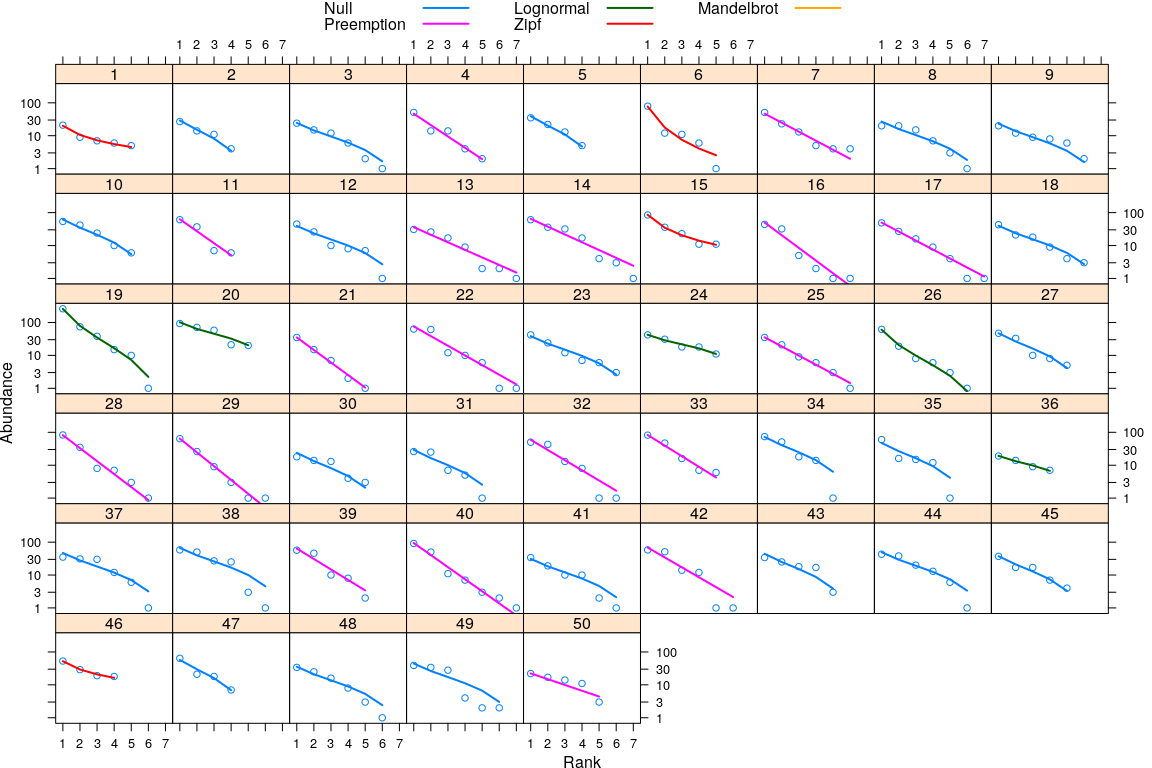
\includegraphics{modelodeabundancia.png}
\caption{Modelo de abundancia de especies \label{fig:modelo_abundancia}}
\end{figure}

La diversidad alpha en el agrupamiento \emph{Ward}, según los modelos de
estimación de riqueza (\emph{Homogeneous model}, estándar y MLE; los
Chao y los Jacknife) se alcanzó la completitud de muestra al 100\% para
los grupos 1, 2 y 4 (1882, 1205 y 1939 individuos, respectivamente) y al
98\% para el grupo 3 (grupo con la menor abundancia, 553 individuos).
Las estimaciones de la diversidad con muestras enrarecidas y
extrapoladas mostraron que en los grupos \emph{Ward} la riqueza máxima
fue alcanzada(ver figuras \ref{fig:asintotico_ward1},
\ref{fig:asintotico_ward2}, \ref{fig:asintotico_ward3} y
\ref{fig:asintotico_ward4}); y para las estimaciones de diversidad
asintótica junto con estadísticas relacionadas (Riqueza de especies,
diversidad de Shannon, y diversidad de Simpson) la riqueza máxima fue
estimada y observada (ver figura \ref{fig:sintotico_ward}).

\begin{figure}
\centering
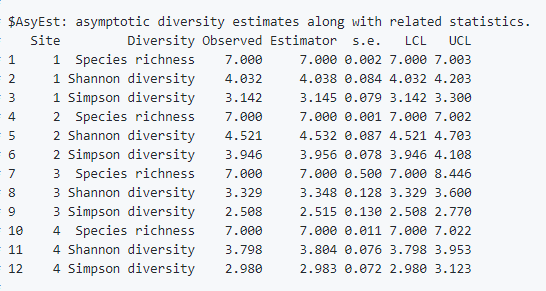
\includegraphics{sintotico_ward.png}
\caption{Resultado de las estimaciones de diversidad asintótica junto
con estadísticas relacionadas, para el agrupamiento \emph{Ward}
\label{fig:sintotico_ward}}
\end{figure}

\emph{C. schippii} y \emph{E. oerstediana} fueron las especies que
hicieron contribución a la diversidad beta, éstas están bien
representadas (la primera con gran dominancia) en los sitios 14 y 19
(grupo 3 \emph{Ward}) que hicieron contribución a la diversidad beta
(ver figura \ref{fig:beta_div}); el 14 fue uno de los cinco sitios que
poseen la riqueza máxima (los demás sitios son 13, 17, 22 y 40) y el 19
fue el sitio más abundante con 399 individuos, de los cuales 261
pertenecían a \emph{C. schippii} (ver figura \ref{fig:abun_sp_q}).
Además, los sitios 14 y 19 están ubicados uno al lado del otro
geográficamente (ver figura \ref{fig:mapa_ward}).

\begin{figure}
\centering
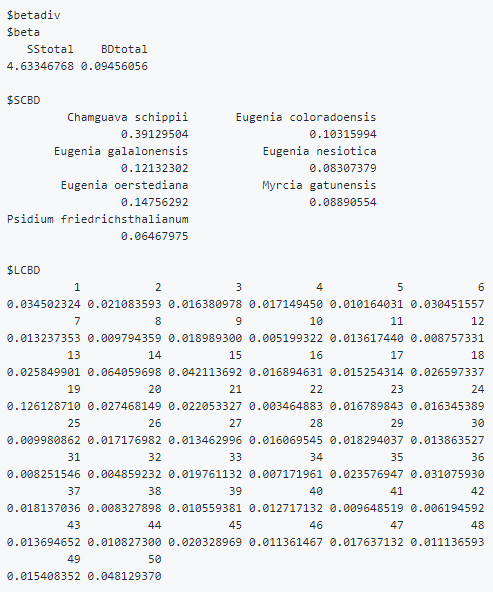
\includegraphics{beta_div.png}
\caption{Resultado de los análisis del SCBD y LCBD\label{fig:beta_div}}
\end{figure}

En los análisis de ecología espacial, la autocorrelación espacial
mediante la prueba de Mantel mostró que hay correlación espacial
inducida por alguna variable en términos positivos para el primer orden
y en términos negativos para el tercer y sexto orden (hasta 500 metros)
(ver figura \ref{fig:prueba_mantel}). Según la prueba I de Moran global
aplicada a abundancia de especies transformadas sin tendencia, \emph{C.
schippii}, \emph{E. oerstediana} y \emph{E. nesiotica} presentaron alta
correlación espacial, y otras como \emph{M. gatunensis}, \emph{E.
galalonensis} y \emph{P. friedrichsthalianum} mostraron un patrón
espacial aleatorio (ver figuras \ref{fig:moranglobal1} y
\ref{fig:moranglobal2}). Además, comparando con los correlogramas del I
de Moran, se observaron patrones espaciales muy parecidos para \emph{C.
schippii}, \emph{B} y \emph{Ca}; para \emph{E. oerstediana} y \emph{N};
y para \emph{E. nesiotica} y \emph{Mn} (ver figuras
\ref{fig:imoran_especies} y \ref{fig:imoran_variables}). Esto coincide
con la prueba del I de Moran local (aplicado a variables ambientales) y
los mapas de \emph{clusters} LISA (aplicado a abundancias de especies
transformadas sin tendencia), \emph{C. schippii} presentó correlación
espacial con los valores de abundancia altos de \emph{Al}, y bajos de
\emph{B}, \emph{Zn}, \emph{Ca} y \emph{N}; \emph{E. oerstediana} mostró
una correlación espacial con los valores de abundancia bajos de
\emph{N}, \emph{N. min.} y \emph{pH}; y \emph{E. nesiotica} con valores
de abundancia bajos de \emph{Mn}, y altos de \emph{N}, y \emph{pH} (ver
figuras \ref{fig:imoranlocal1}, \ref{fig:imoranlocal2} y
\ref{fig:imoranlocal3}).

\begin{figure}
\centering
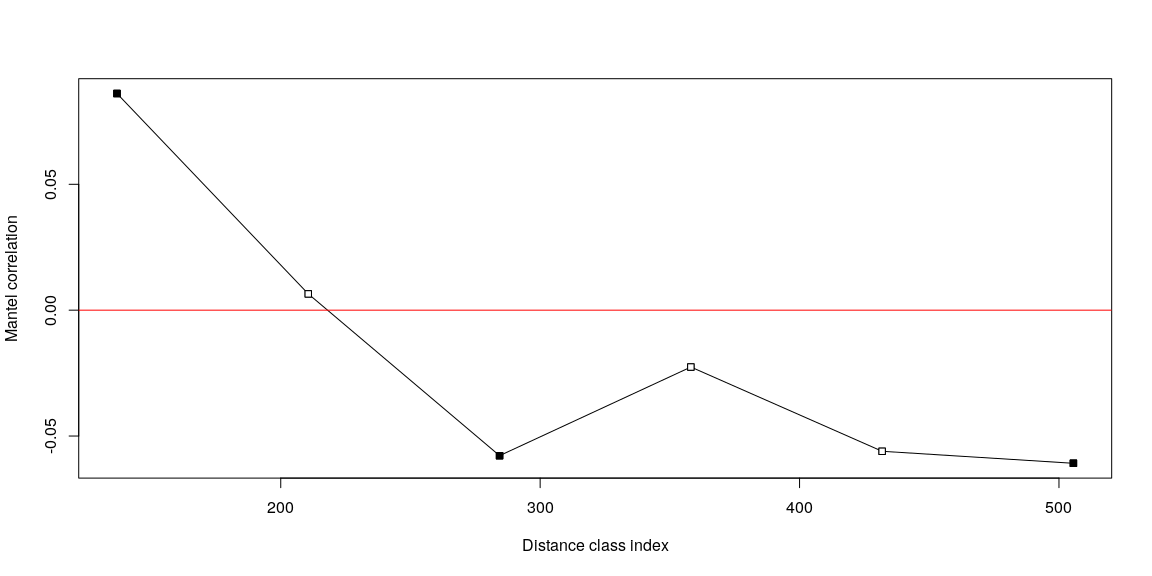
\includegraphics{prueba_mantel.png}
\caption{Autocorrelación espacial mediante prueba Mantel (matrices de
distancia) \label{fig:prueba_mantel}}
\end{figure}

\begin{figure}
\centering
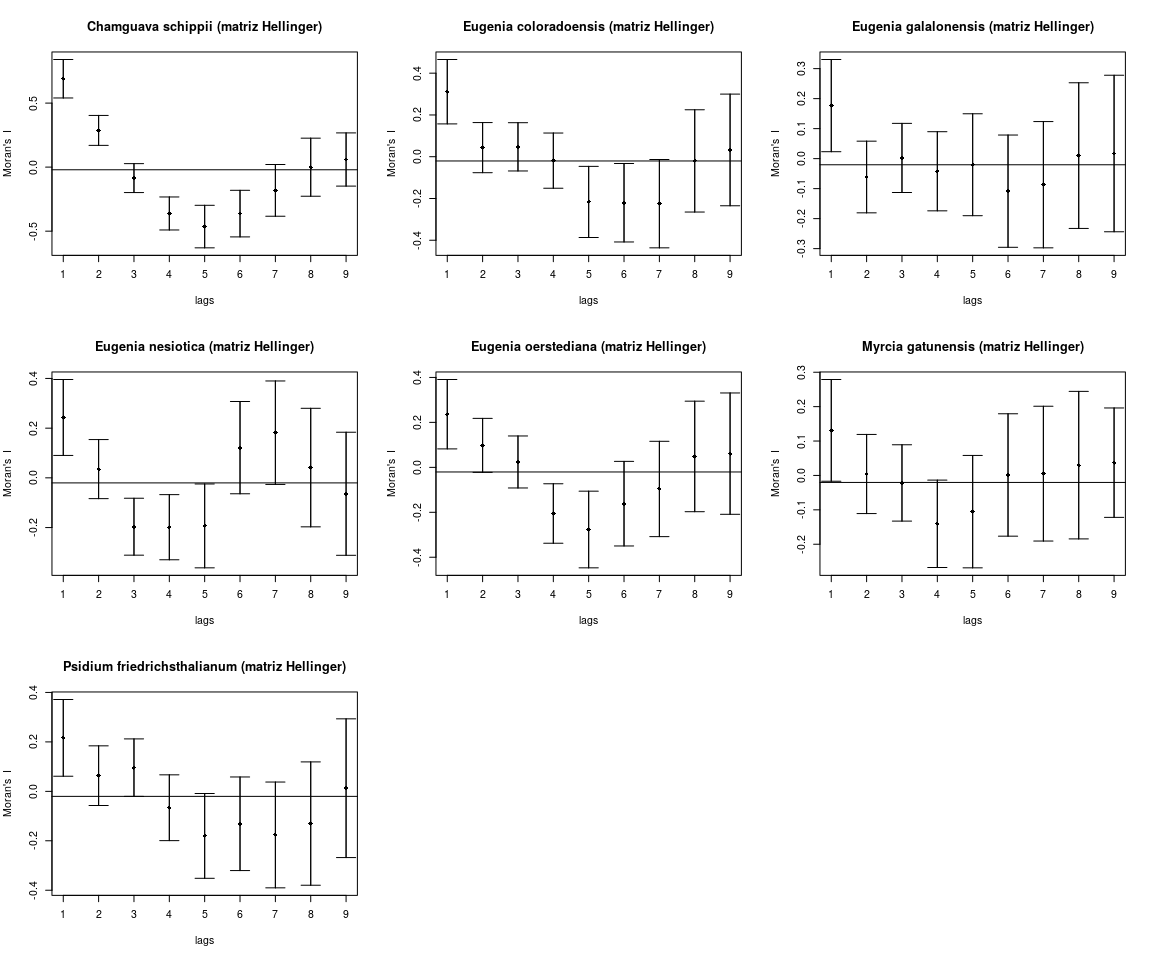
\includegraphics{imoran_especies.png}
\caption{Correlograma, I de Moran con abundancias de especies
\label{fig:imoran_especies}}
\end{figure}

\begin{figure}
\centering
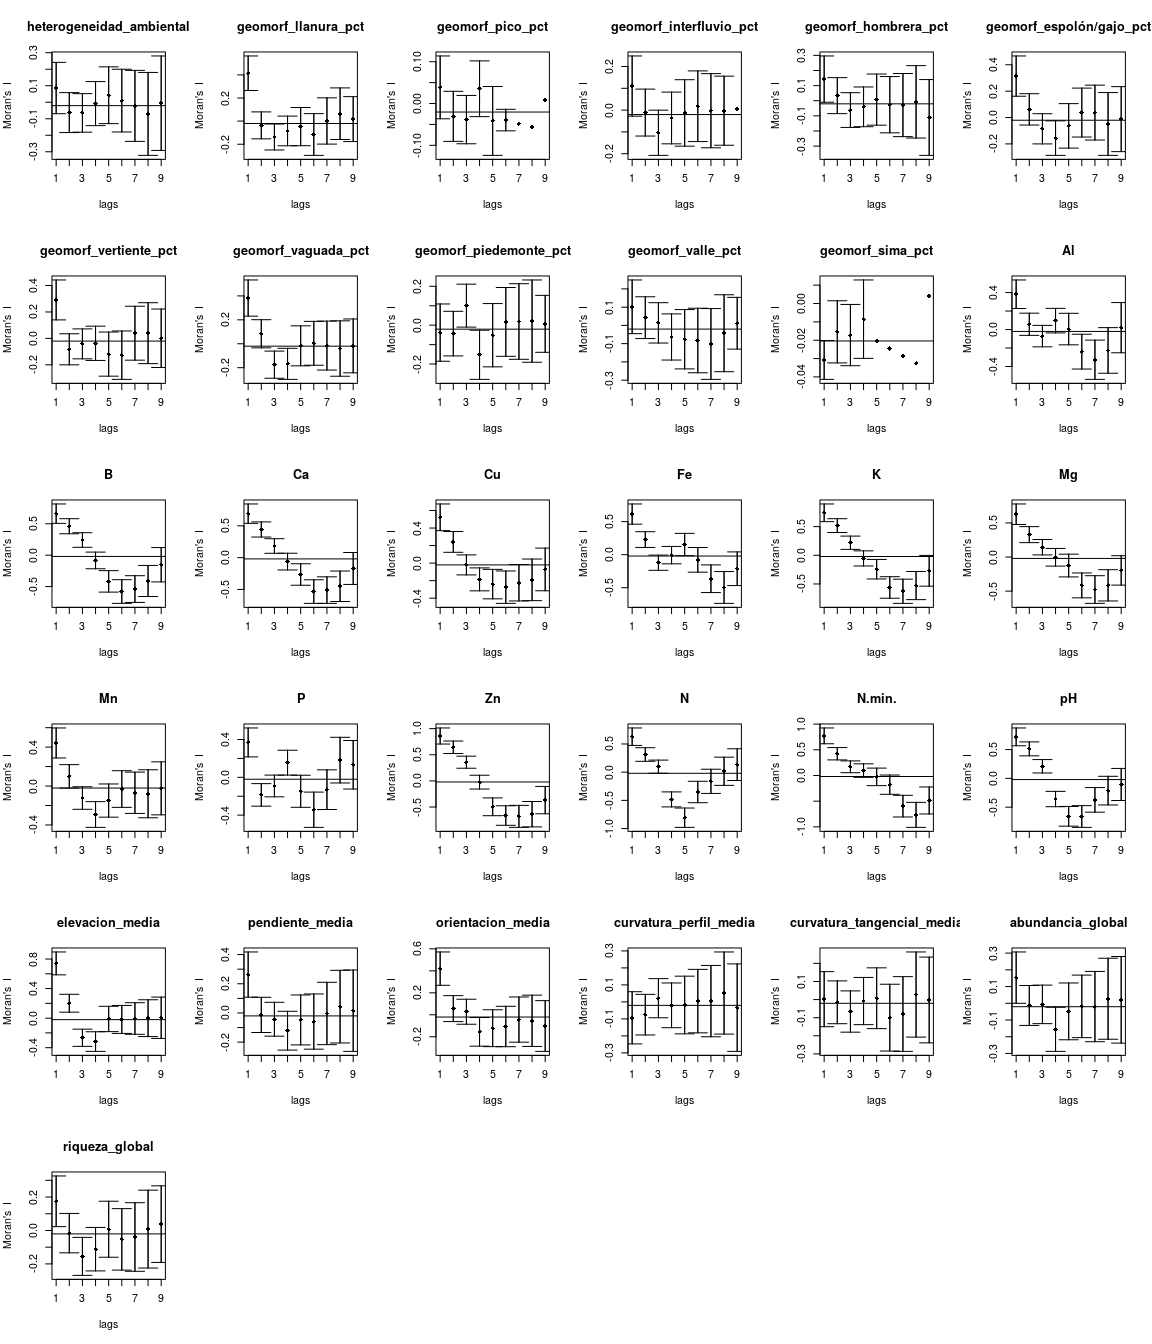
\includegraphics{imoran_variables.png}
\caption{Correlograma, I de Moran con variables ambientales
\label{fig:imoran_variables}}
\end{figure}

\section{Discusión}\label{discusiuxf3n}

Las mirtaceas de la parcela permanente de BCI presentaron una riqueza de
7 especies y 4 géneros pertenecientes a la subtribu Myrteae. El 57\% de
esta riqueza, correspondiente a las especies del género \emph{Eugenia},
presentaron altos grados de asociación entre ellas, por lo que supone un
patrón de dependencia, a diferencia de las especies \emph{P.
friedrichsthalianum}, \emph{M. gatunensis} y \emph{C. schippii}
mostraron un patrón independiente, por lo que supone que se presentan
aleatoriamente en la muestra sin asociarse a las otras especies.

Las Myrteae de esta muestra, según el método \emph{Ward}, se dividen en
4 grupos, cada uno con 20, 13, 2 y 15 sitios respectivamente. Este
agrupamiento, según las pruebas ANOVA y Kruskal-Wallis y el diagrama de
cajas, estuvo influenciado por variables de suelo: \emph{pH, Cu, Zn, Ca,
Mg, N, Al} y \emph{K}; y atributos del terreno: pendiente\_media,
orientacion\_media, elevación\_media, geomorf\_espolon/gajo\_pct. El
grupo 3 (con 2 sitios, 14 y 19) coincide en los métodos de agrupamiento
(\emph{single}, \emph{complete}, UPGMA y \emph{Ward}) y el remuestreo de
\emph{bootstrap} multiescalar (BP de 76\% y un AU de 99\%) esto infiere
que es un grupo natural y real dentro de la localidad.

Según el análisis de especies indicadoras (IndVal), las especies
asociadas como diagnósticas para el agrupamiento \emph{Ward}, fueron
\emph{C. schippii} para el grupo 3, \emph{E. coloradoensis} para el
conjunto 1+2 y \emph{E. oerstediana} para el grupo 3+4. También,
\emph{C. schippii} presentó preferencia por los hábitats del grupo 3,
\emph{E. coloradoensis} para los del grupo 2, y \emph{E. oerstediana}
para los del grupo 4. Esto puede ser debido a las altas abundancias de
estas especies presentes en estos grupos.

El modelo de abundancia de especies muestra que el 56\% de la comunidad
presenta mayores valores de equidad (log normal 10\% y null 46\%). No
obstante, los estimadores de riqueza mostraron que la completitud de
muestra para las mirtáceas en estudio fue estimada y observada al 100\%,
lo mismo para los grupos \emph{Ward}. De lo que se infiere, que este es
un patrón natural de las Myrteae, y no será necesario aumentar el
esfuerzo de muestreo porque no se espera encontrar más especies de esta
familia en BCI.

La riqueza y abundancia de la familia presentó asociación estadística en
términos positivos con \emph{Al}, \emph{P} y en términos negativos con
\emph{Ca}; y la abundancia presentó asociación estadística en términos
positivos con \emph{Al} y elevación media, y en términos negativos con
\emph{Ca}, heterogeneidad ambiental y geomorfología de vaguada. Además,
la diversidad alpha de las comunidad presentó correlación con las
variables \emph{Al, P, Ca, Fe} y la geomorfología de pendiente media. De
lo que se infiere, que la presencia de estas variables está relacionada
estrechamente con la distribución de la familia en la parcela permanente
de BCI.

Las especies que hacen contribución a la diversidad beta fueron \emph{C.
schippii} y \emph{E. oerstediana}, y los sitios que hacen contribución
fueron los sitios 14 y 19 (grupo \emph{Ward} 3). Este grupo posee altas
abundancias de las especies antes mencionadas; el sitio 19 posee la
mayor abundancia de especies por quadrat, 399 individuos de los cuales,
261 son de \emph{C. schippii} y 38 de \emph{E. oerstediana}; y el sitio
14 posee 154 individuos, de los cuales 61 son de \emph{C. schippii} y 32
de \emph{E. oerstediana}. Estos sitios se encuentran juntos
geográficamente, y presentan altos grados de \emph{Al} y bajos grados de
\emph{N}, lo que según los análisis de ecología espacial se relaciona
con altas abundancias de las especies antes mencionadas.

Los análisis de ecología espacial de mirtáceas, mediante la prueba de
Mantel, mostraron estadísticamente que hay correlación espacial inducida
por alguna variable en términos positivos para el primer orden. Las
especies \emph{C. schippii}, \emph{E. oerstediana} y \emph{E. nesiotica}
presentaron alta correlación espacial; y \emph{M. gatunencis}, \emph{E.
galalonensis} y \emph{P. friedrichsthalianum} presentaron un patrón
aleatorio. Con la prueba del I de Moran local (aplicado a variables
ambientales) y los mapas de \emph{clusters} LISA (aplicado a abundancias
de especies transformadas sin tendencia), se evidenció estadísticamente
que ésta correlación para \emph{C. schippii} está inducida por los
valores de abundancia altos de \emph{Al}, y bajos de \emph{B},
\emph{Zn}, \emph{Ca} y \emph{N}; para \emph{E. oerstediana} por los
valores de abundancia bajos de \emph{N}, \emph{N. min.} y \emph{pH}; y
para \emph{E. nesiotica} por los valores de abundancia bajos de
\emph{Mn}, y altos de \emph{N}, y \emph{pH}.

\subsection{Interpretación}\label{interpretaciuxf3n}

De los resultados obtenidos, se obtienen nuevos conocimientos
preliminares de las especies de mirtáceas que se desarrollan a
continuación:

-La distribución de las Myrteae en la parcela permanente de BCI presenta
una estrecha relación con las variables \emph{Al, P, Ca, Fe} y la
geomorfología de pendiente media.

-\emph{P. friedrichsthalianum} y \emph{M. gatunensis} son especies raras
que no se asocian con otras mirtáceas, presentan patrones aleatorios.
Además, \emph{M. gatunensis} fue descrita en Barro Colorado por Standl,
se infiere que es preliminarmente endémica del área del lago Gatún
(Kenoyer, Standley, Howe, \& Dahlgren, 1929).

-\emph{C. schippii} es una especie que no se asocia con otras mirtáceas.
Su abundancia puede aumentar en presencia altos valores de \emph{Al} y
bajos \emph{B}, \emph{Zn}, \emph{Ca} y \emph{N}. Se infiere que es
preliminarmente basófila.

-Las especies del género \emph{Eugenia} presentan un patrón de
dependencia. Además, se infiere que \emph{E. oerstediana} es
preliminarmente basófila y \emph{E. nesiotica} preliminarmente
acidófila.

\subsection{Limitaciones y futuro}\label{limitaciones-y-futuro}

Los datos de BCI son censales, por lo que el sesgo de muestreo es una
preocupación menor. Sin embargo, los datos de BCI también tienen sesgo,
debido a que se utiliza un DAP de corte para decidir si un individuo es
censado o no. No obstante, los datos censales carecen de una fortaleza
porque no reflejan asociación con grandes unidades de hábitats y,
además, revelan asociación con microhábitats muy específicos, por lo que
extraer conclusiones sobre patrones de asociación con variables
ambientales de manera más general, presenta sus limitaciones. Debido a
esto se nesecitarán más estudios de estas mirtáceas en otros hábitats
menos relacionados para observar verdaderos patrones naturales y ver si
coinciden con los de este estudio, que se han quedado en la estadística
inferencial.

Otra de las limitaciones, es que no se encontraron estudios que
respalden o no los resultados de este estudio, debido a que las
preferencias de las especies de Myrteae de la parcela permanente de BCI
han sido muy poco estudiadas. Se necesitarán más estudios sobre
preferencias de variables ambientales y hábitats.

\section{Agradecimientos}\label{agradecimientos}

Primero, al profesor José R. Martínez por toda su paciencia, motivación
y excelentes correcciones durante el proceso.

A mi compañero de clase, colega y amigo, Marcos A. González por leer mi
trabajo, corrigerme algunas faltas ortográficas, señalarme otras de
sentido, motivarme y apoyarme siempre.

A mi familia, que me apoyaron, fueron pacientes y entenderieron que
debía pasar muchas horas despierta haciendo el trabajo y dejar de
atender otras responsabilidades para alcanzar mi objetivo.

A Ruth H. Bastardo, maestra y asesora de tesis, por sus consejos y
motivación siempre.

Mis más grato agradecimiento a todos, por ayudarme a concluir mi última
materia de carrera.

\section{Información de soporte}\label{informaciuxf3n-de-soporte}

\beginsupplement

\begin{figure}
\centering
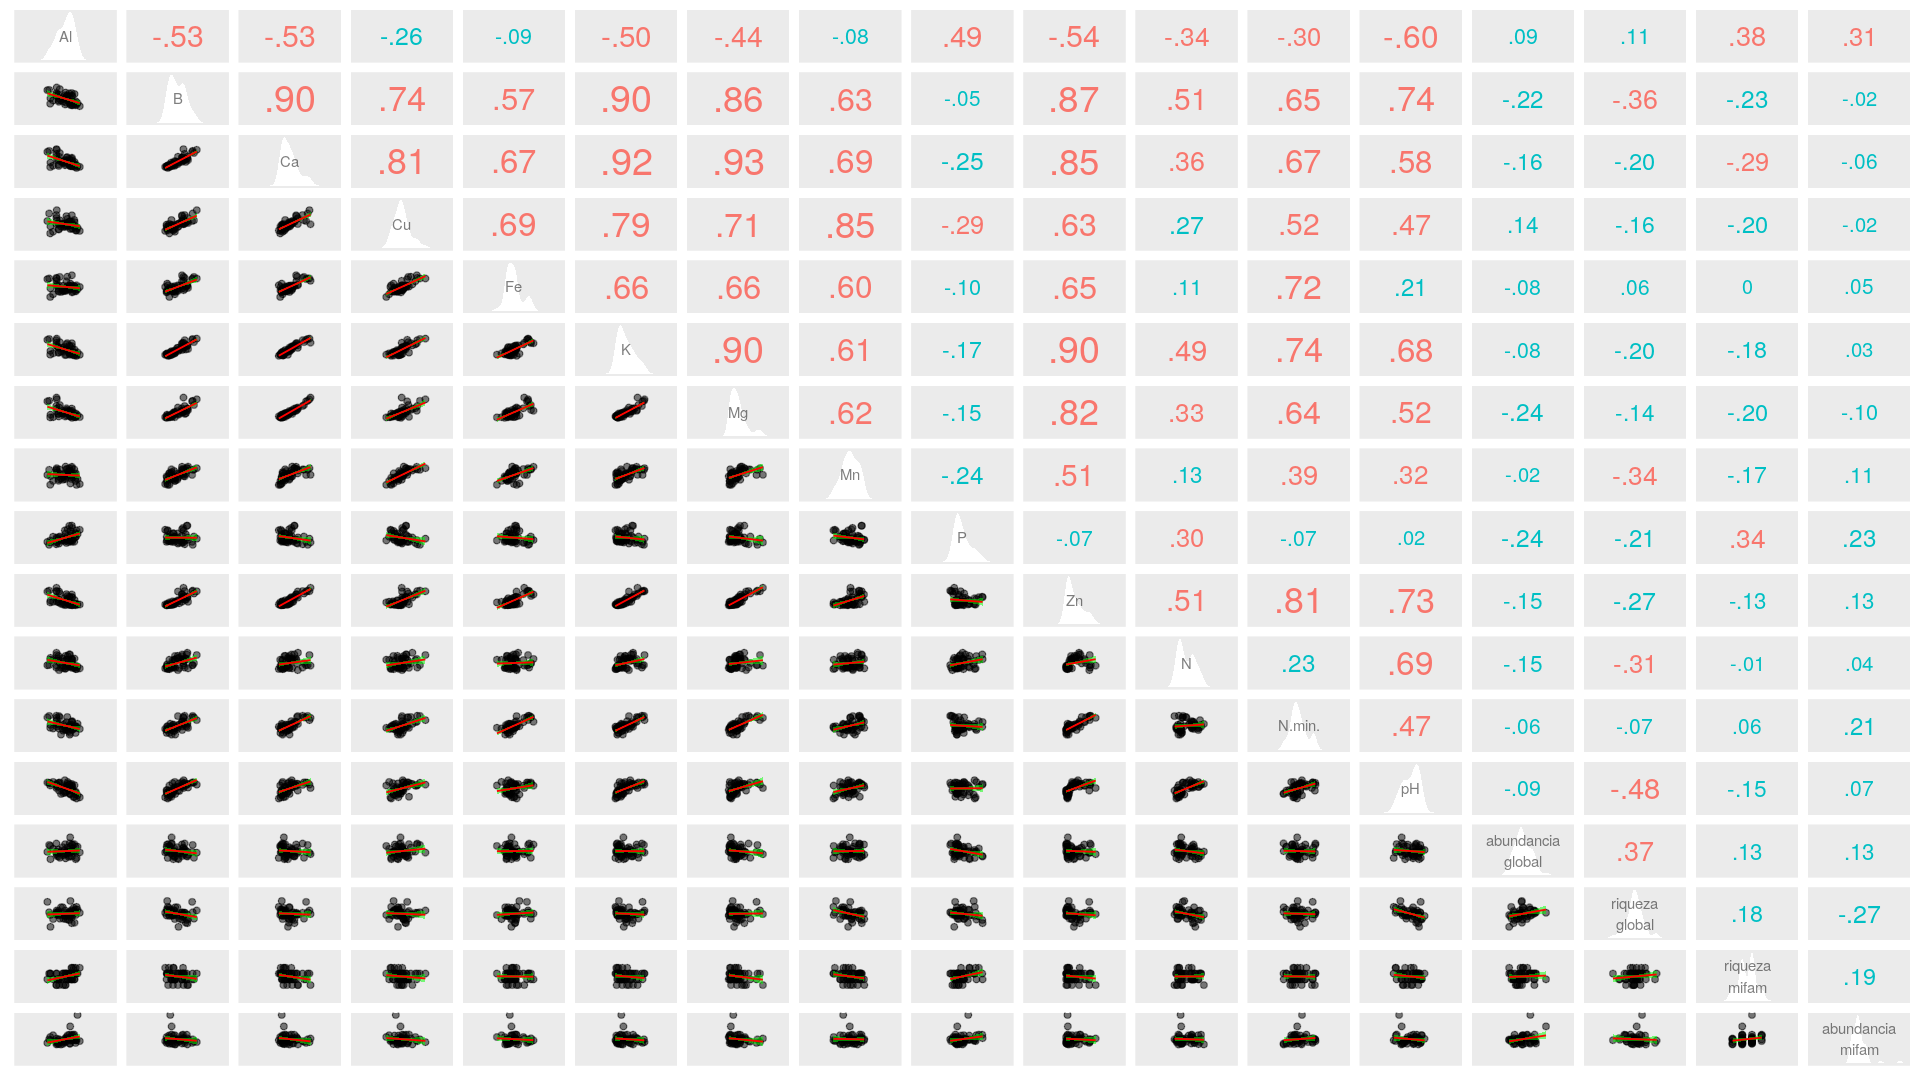
\includegraphics{matriz_correlacion_suelo_abun_riq_spearman.png}
\caption{Matriz de correlación, índice de Spearman
\label{fig:matriz_spearman}}
\end{figure}

\begin{figure}
\centering
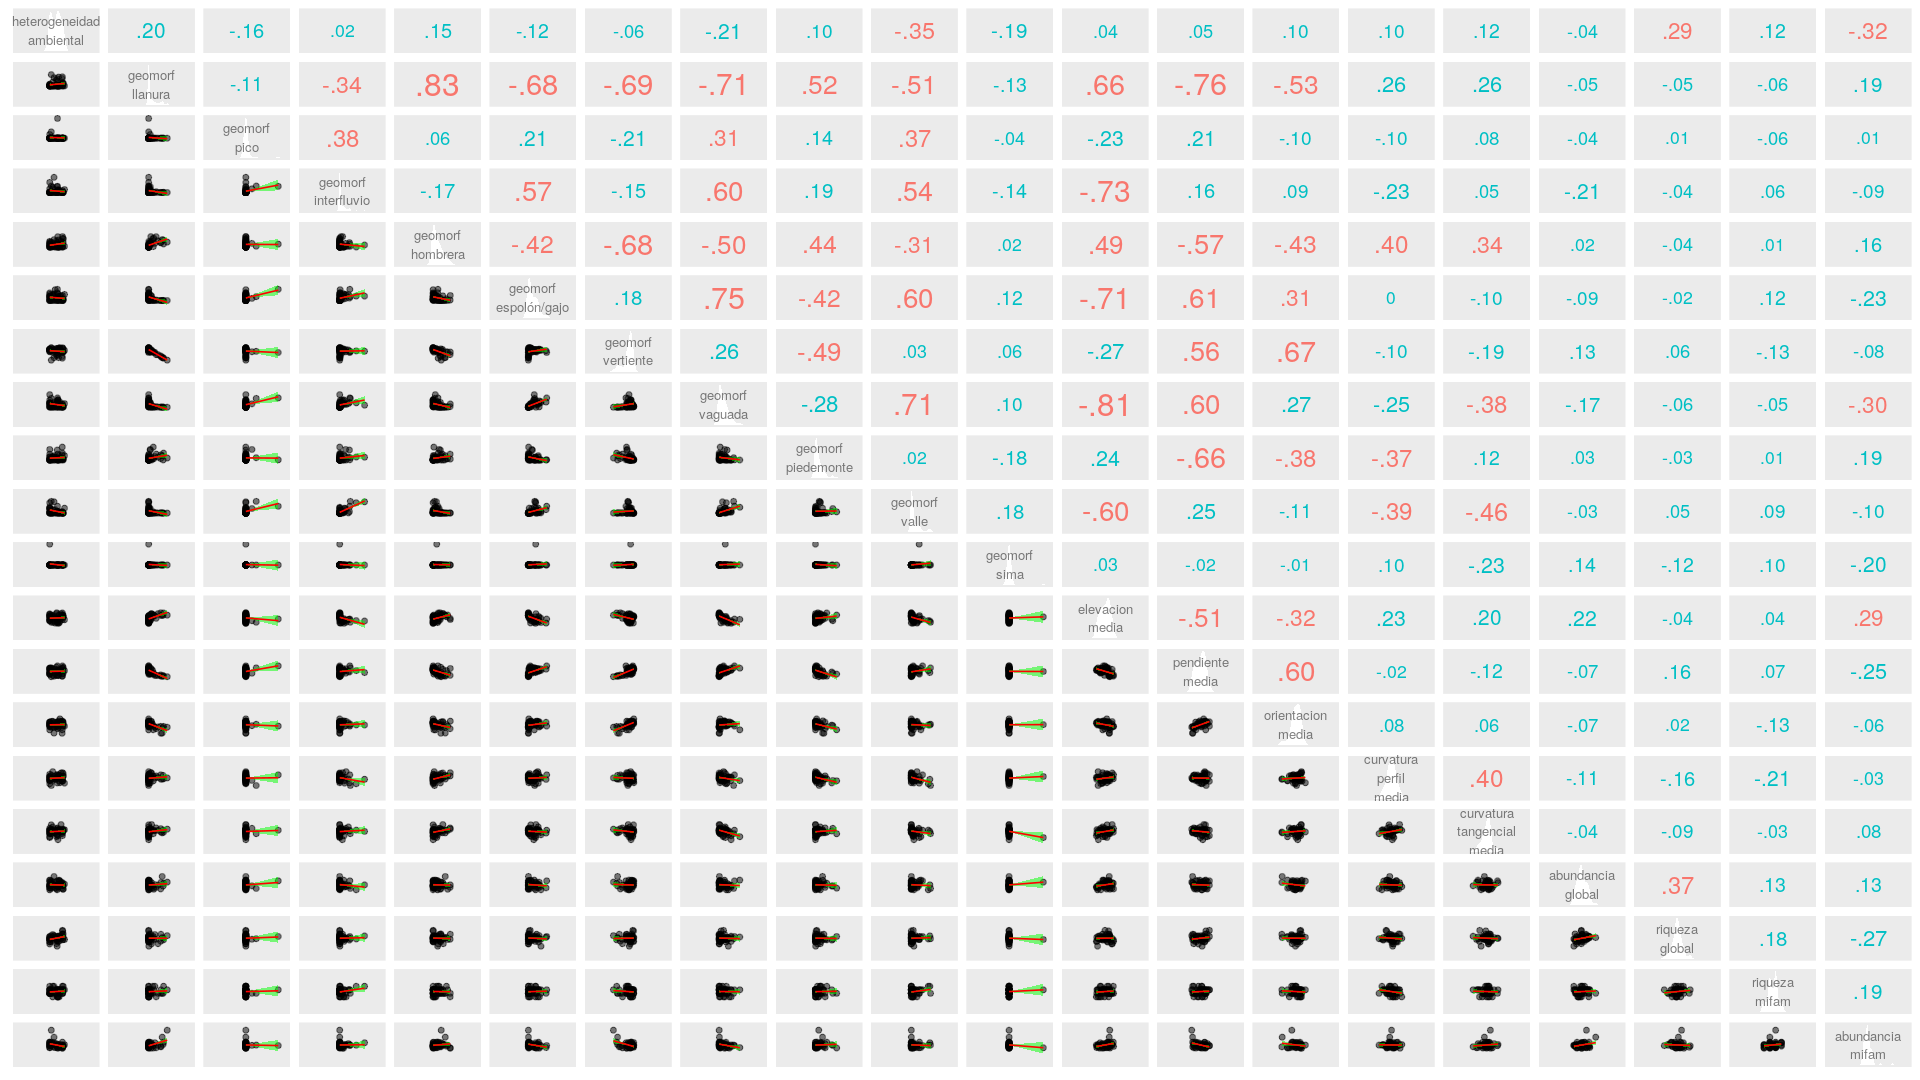
\includegraphics{matriz_correlacion_geomorf_abun_riq_spearman.png}
\caption{Matriz de correlación, índice de Pearson
\label{fig:matriz_pearson}}
\end{figure}

\begin{figure}
\centering
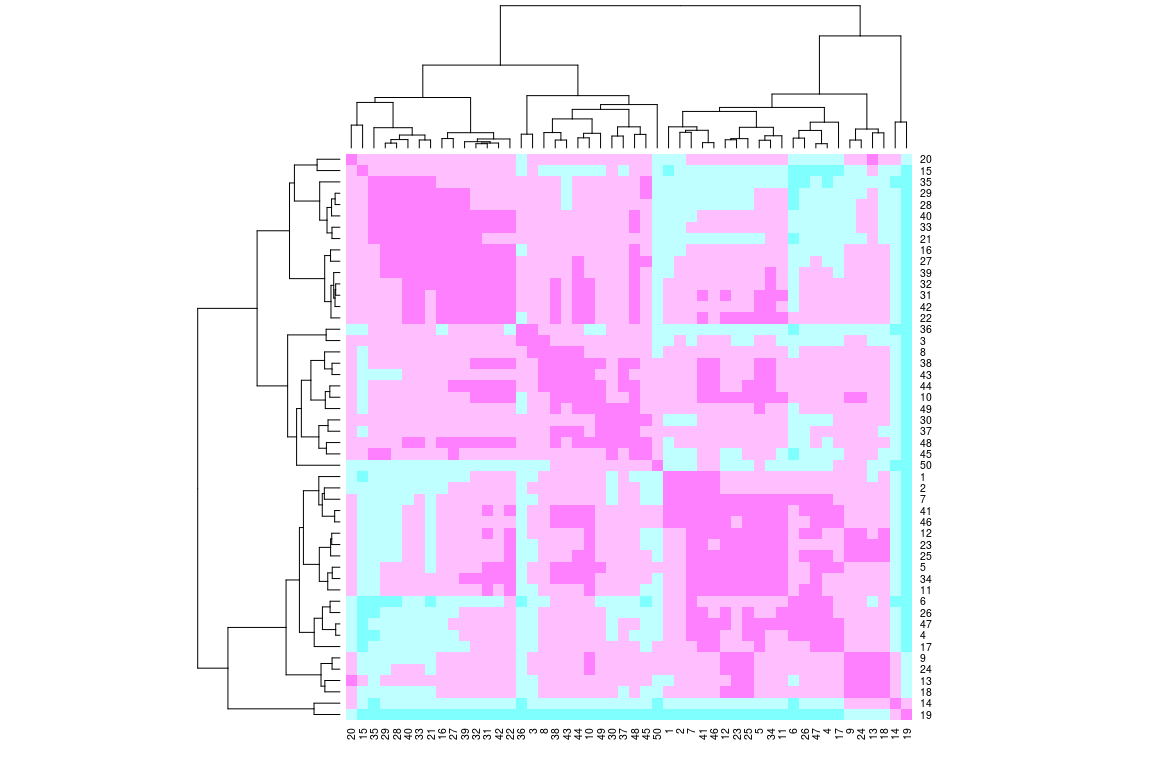
\includegraphics[width=0.50000\textwidth]{Mapadecalor_Ward_aa2.png}
\caption{Mapa de calor con el dendrograma del agrupamiento \emph{Ward}
\label{fig:mapadecalor_ward}}
\end{figure}

\begin{figure}
\centering
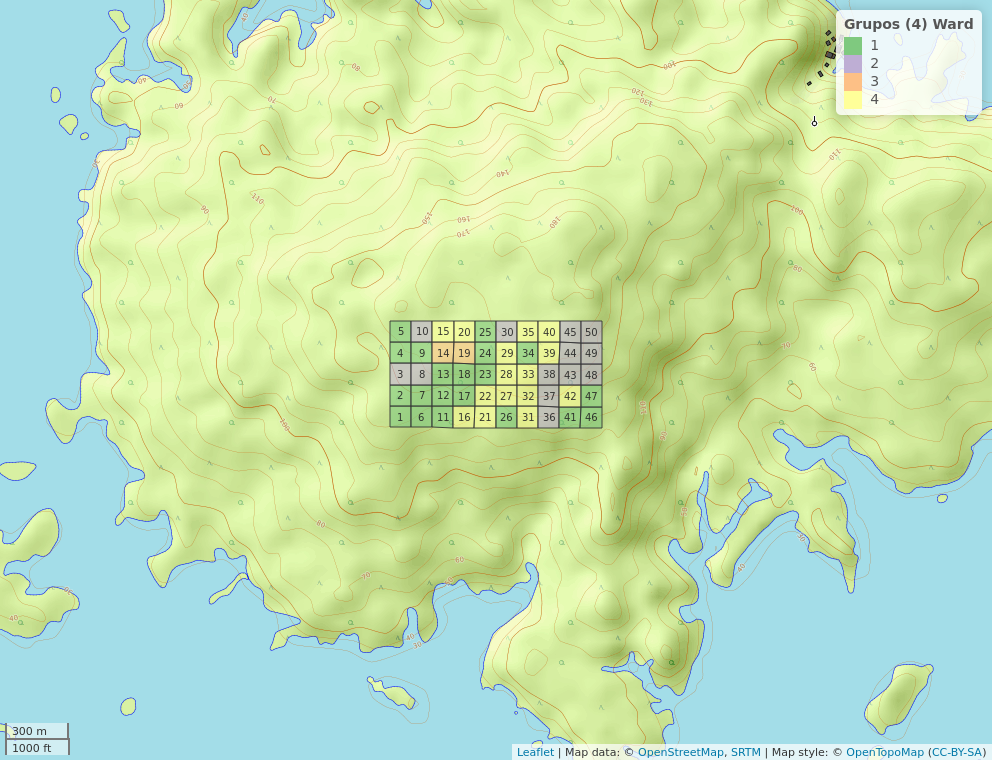
\includegraphics[width=0.50000\textwidth]{mapa_ward_k4.png}
\caption{Agrupamiento por el método \emph{Ward} de varianza mínima de
las mirtáceas \label{fig:mapa_ward}}
\end{figure}

\begin{figure}
\centering
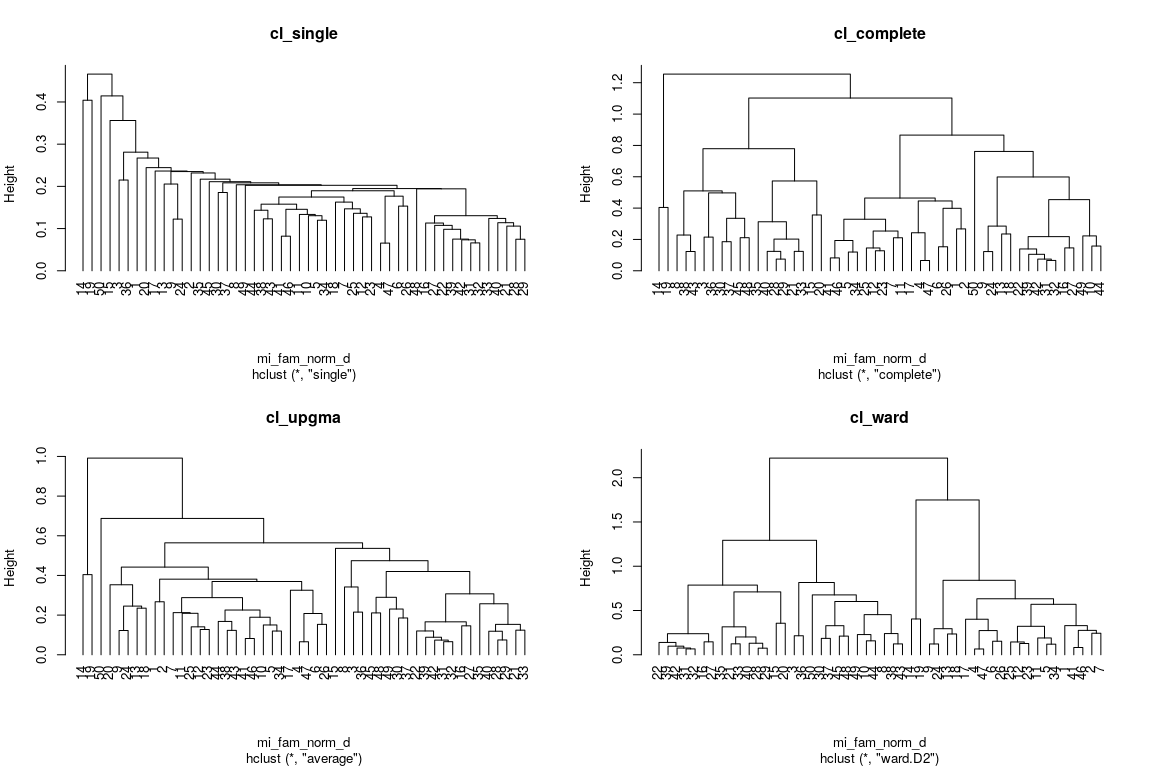
\includegraphics{metodosdeagrupamiento.png}
\caption{Métodos de agrupamiento \label{fig:metodosdeagrupamiento}}
\end{figure}

\begin{figure}
\centering
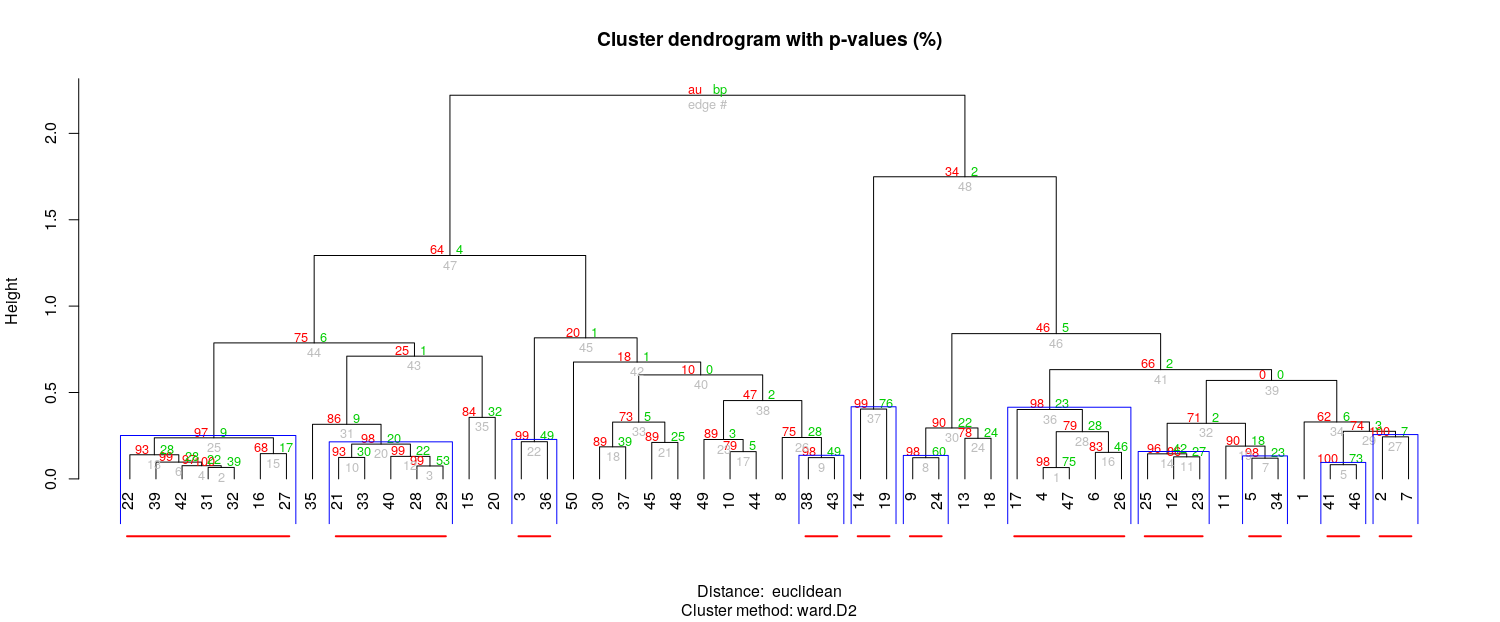
\includegraphics{bootstrap_Ward.png}
\caption{Dendrograma, agrupamiento \emph{Ward} con los porcentajes del
remuestreo de \emph{bootstrap} multiescalar
\label{fig:*bootstrap*_multiescalar}}
\end{figure}

\begin{figure}
\centering
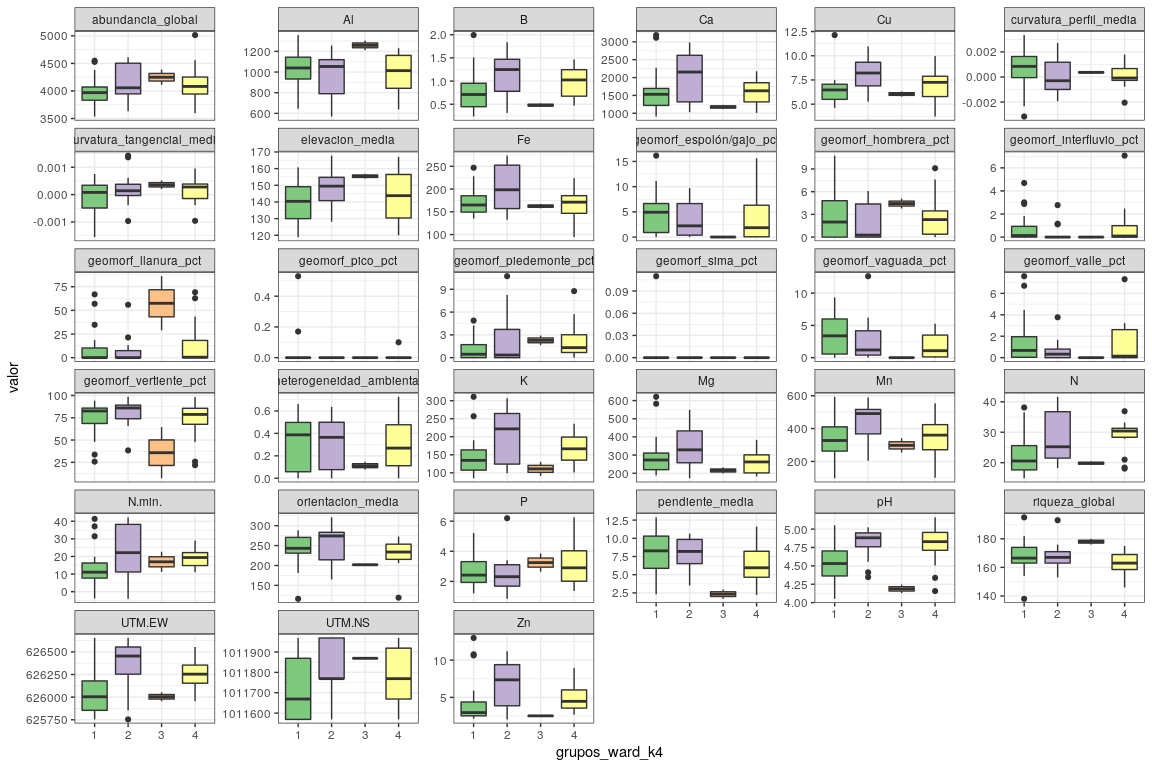
\includegraphics{correlograma_wardyvariablesambientales.png}
\caption{Diagrama de cajas de los grupos \emph{Ward} en relación con
variables ambientales y atributos \label{fig:ward_con_variables}}
\end{figure}

\begin{figure}
\centering
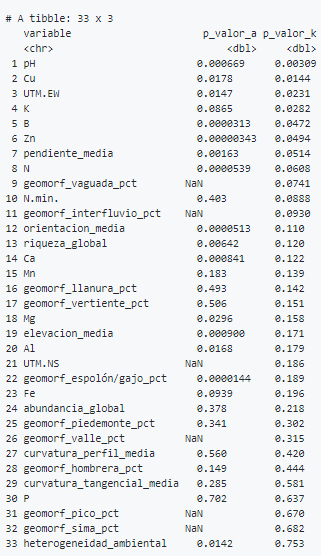
\includegraphics{anova_kruskalwallis_ward.png}
\caption{Pruebas ANOVA y Kruskal-Wallis para el agrupamiento \emph{Ward}
\label{fig:anova_kruskalwallis_ward}}
\end{figure}

\begin{figure}
\centering
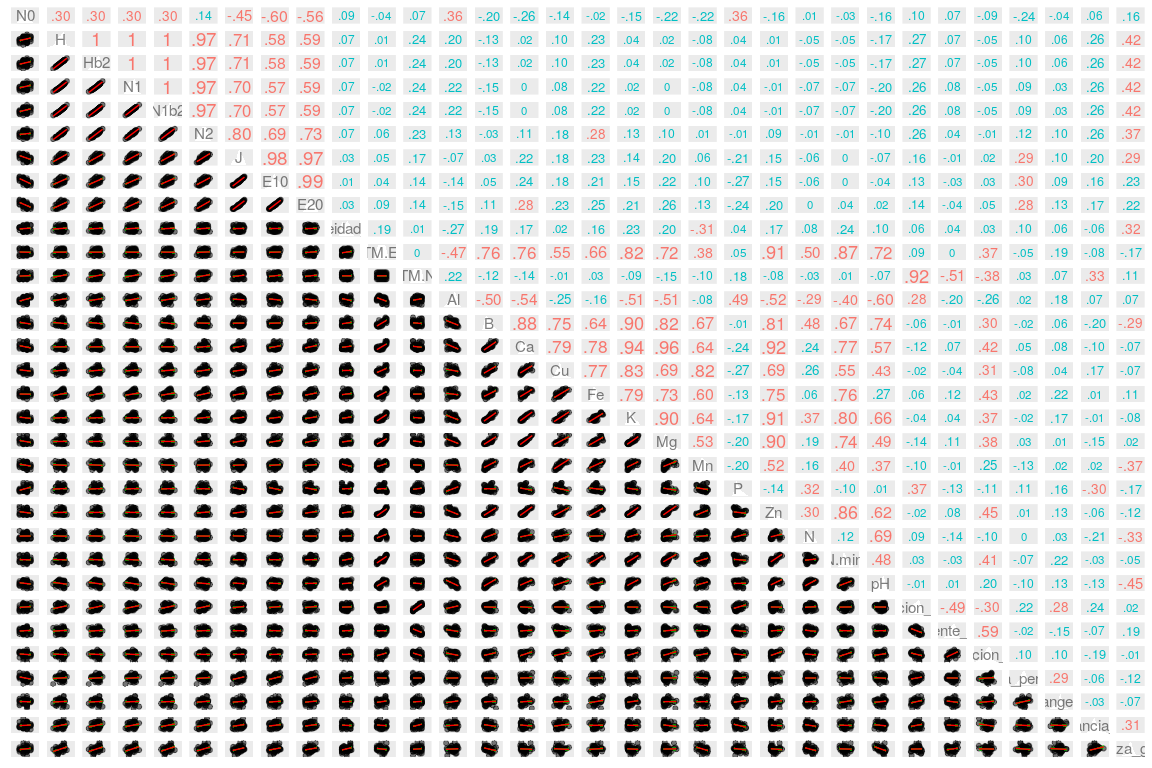
\includegraphics{pearson_indcdiversidad.png}
\caption{Matriz que relaciona los índices de diversidad alpha con las
variables/atributos del suelo \label{fig:pearson_div}}
\end{figure}

\begin{figure}
\centering
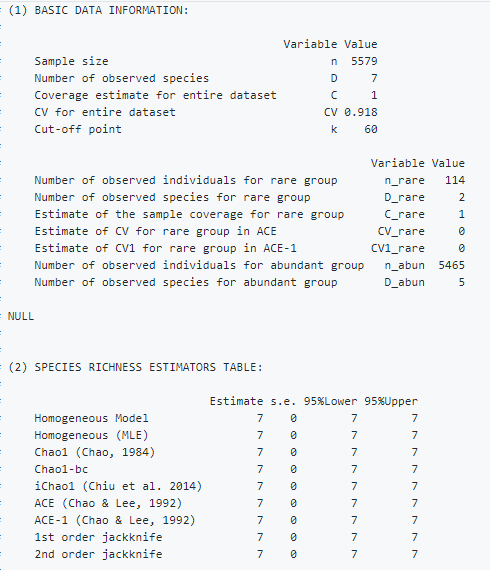
\includegraphics{chao_asintotico.png}
\caption{Resultado de las estimaciones de diversidad para la matriz de
comunidad combinada, en la que todos los sitios forman uno
\label{fig:chao_asintotico}}
\end{figure}

\begin{figure}
\centering
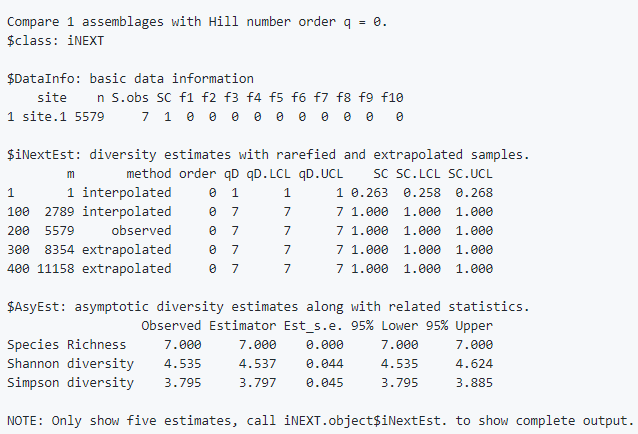
\includegraphics{chao_noasintotico.png}
\caption{Resultado de rarefacción y extrapolación para la matriz de
comunidad combinada en la que todos los sitios forman uno
\label{fig:chao_noasintotico}}
\end{figure}

\begin{figure}
\centering
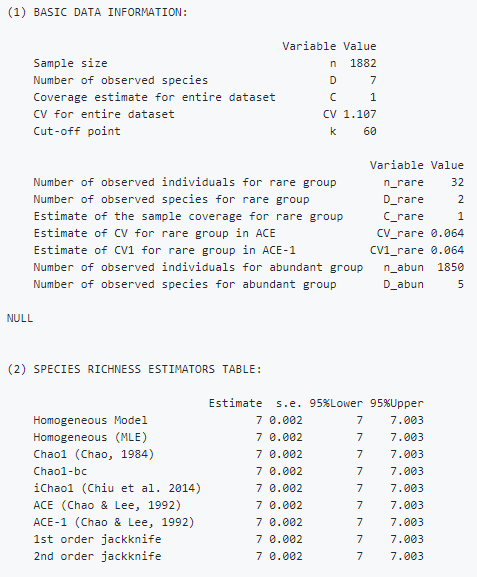
\includegraphics{asintotico_ward1.png}
\caption{Resultado de las estimaciones de diversidad asintótica, grupo
\emph{Ward} 1 \label{fig:asintotico_ward1}}
\end{figure}

\begin{figure}
\centering
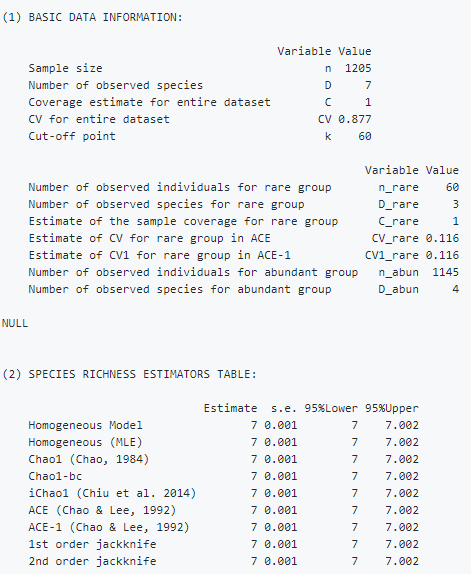
\includegraphics{asintotico_ward2.png}
\caption{Resultado de las estimaciones de diversidad asintótica, grupo
\emph{Ward} 2 \label{fig:asintotico_ward2}}
\end{figure}

\begin{figure}
\centering
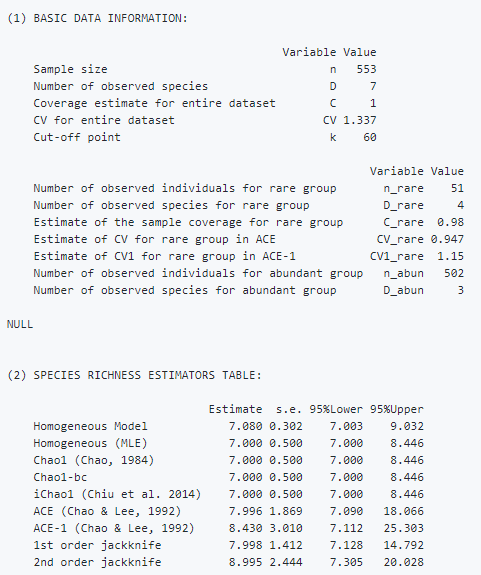
\includegraphics{asintotico_ward3.png}
\caption{Resultado de las estimaciones de diversidad asintótica, grupo
\emph{Ward} 3 \label{fig:asintotico_ward3}}
\end{figure}

\begin{figure}
\centering
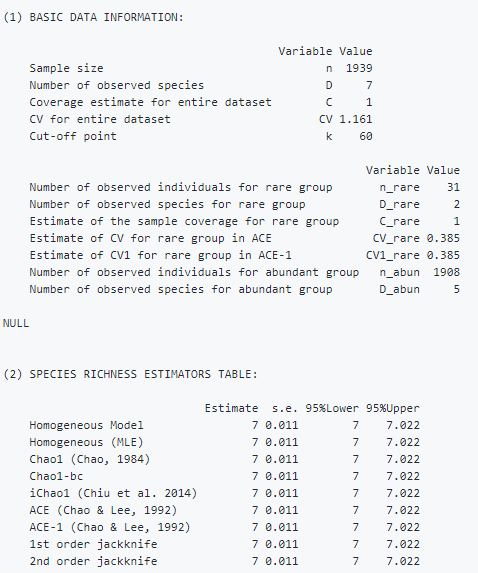
\includegraphics{asintotico_ward4.png}
\caption{Resultado de las estimaciones de diversidad asintótica, grupo
\emph{Ward} 4 \label{fig:asintotico_ward4}}
\end{figure}

\begin{figure}
\centering
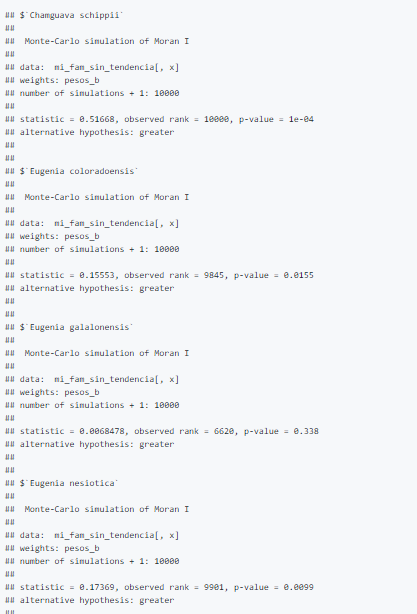
\includegraphics{ee_files/figure-markdown_github/moranglobal1.png}
\caption{I de Moran global aplicado a abundancia de especies
transformadas sin tendencia, parte 1 \label{fig:moranglobal1}}
\end{figure}

\begin{figure}
\centering
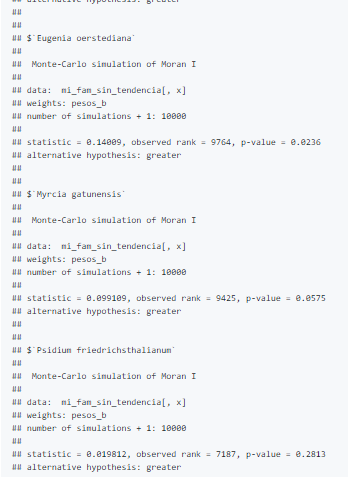
\includegraphics{ee_files/figure-markdown_github/moranglobal2.png}
\caption{I de Moran global aplicado a abundancia de especies
transformadas sin tendencia, parte 2 \label{fig:moranglobal2}}
\end{figure}

\begin{figure}
\centering
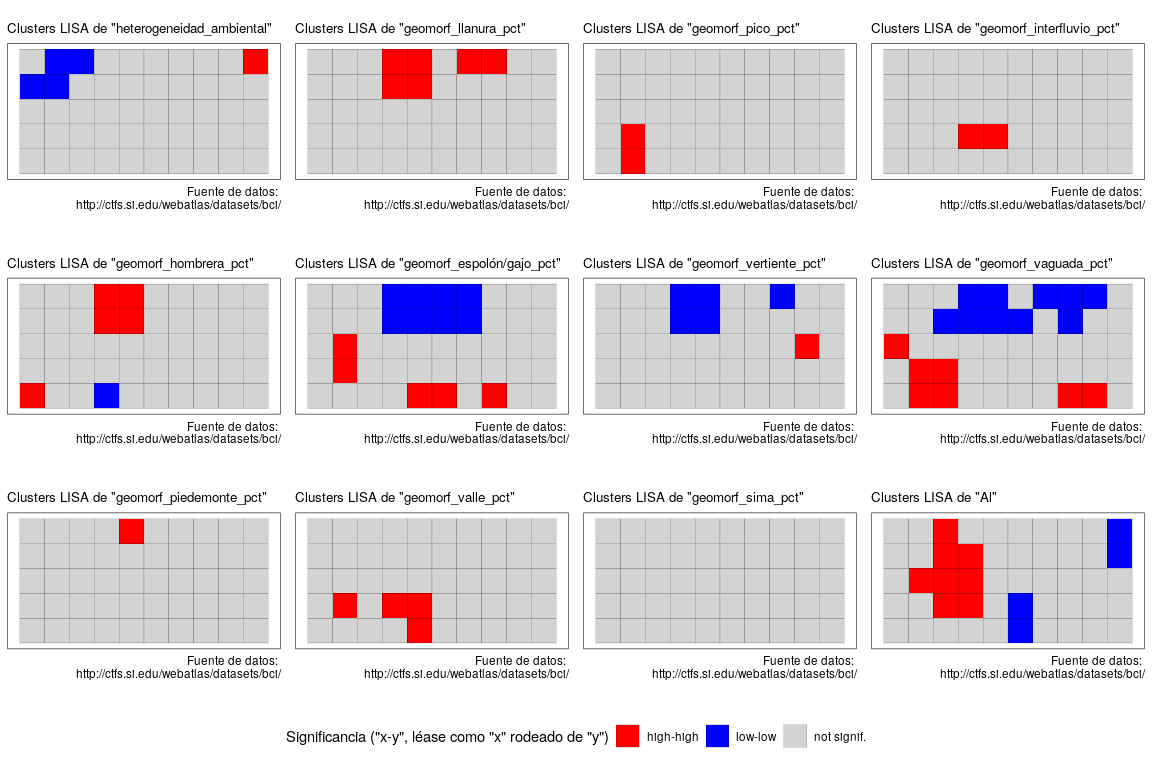
\includegraphics{ee_files/yodemoranlocal-1.png}
\caption{I de Moran local aplicado a variables ambientales, parte 1
\label{fig:imoranlocal1}}
\end{figure}

\begin{figure}
\centering
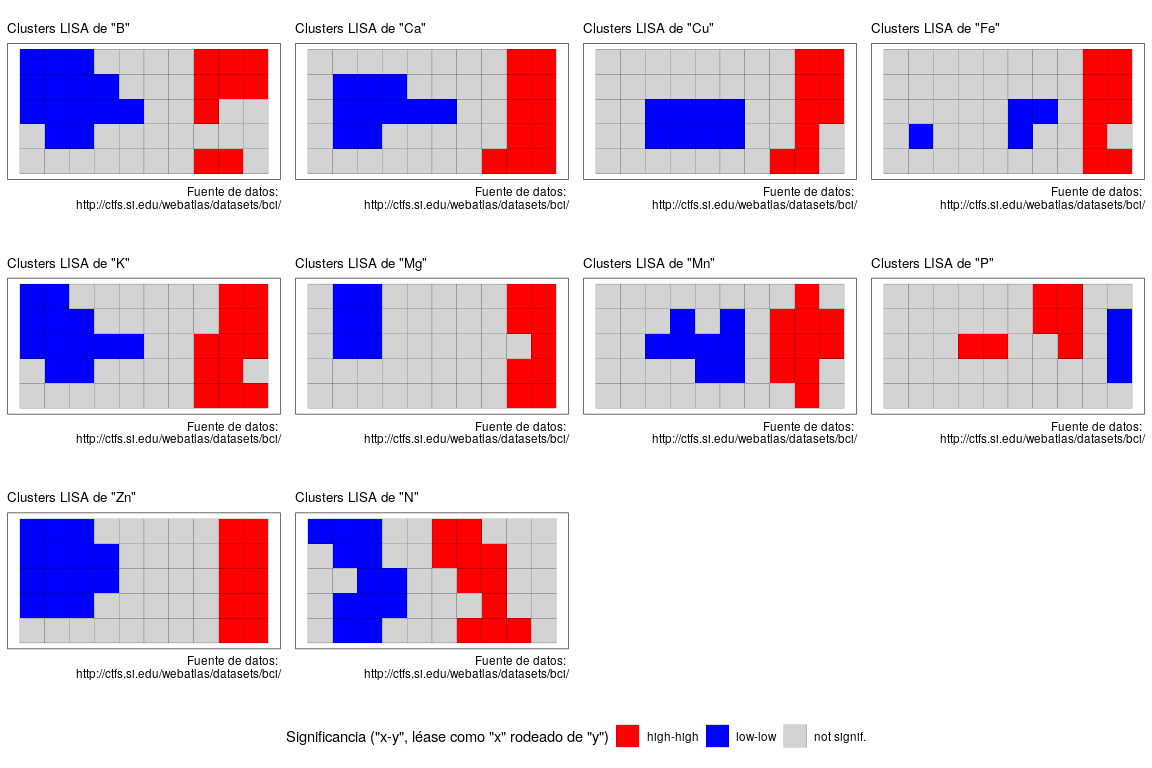
\includegraphics{ee_files/yodemoranlocal-2.png}
\caption{I de Moran local aplicado a variables ambientales, parte 2
\label{fig:imoranlocal2}}
\end{figure}

\begin{figure}
\centering
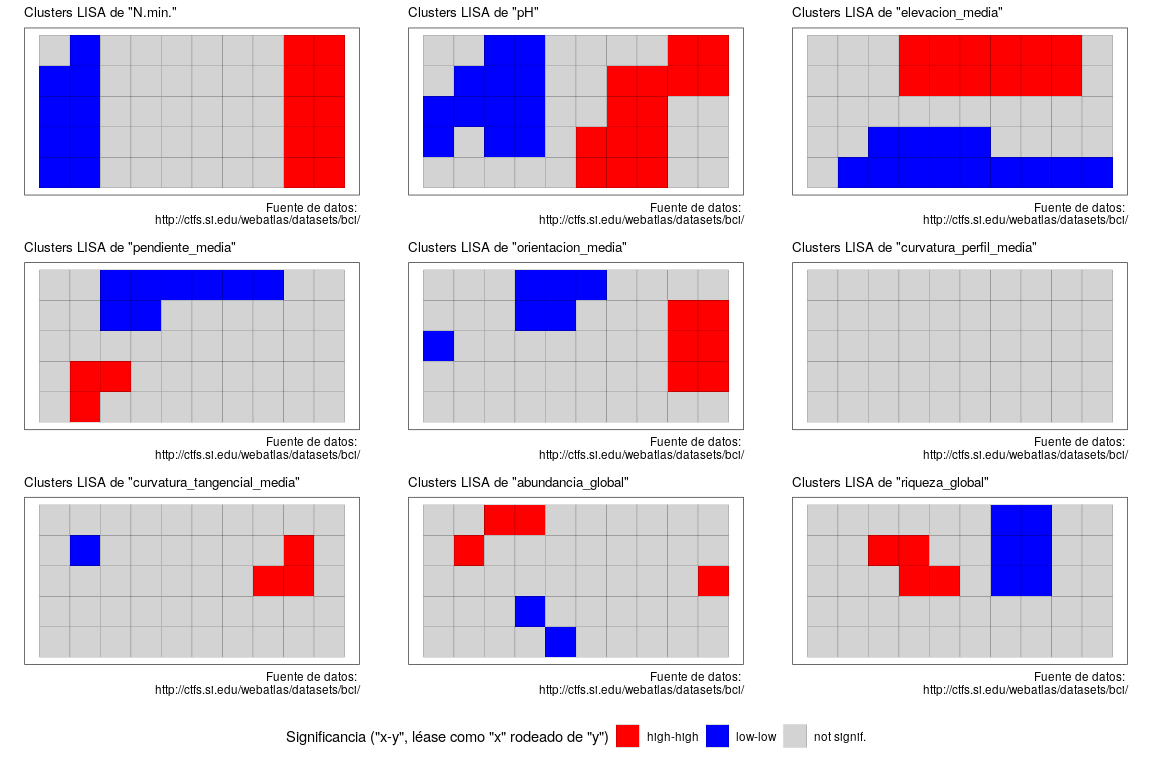
\includegraphics{ee_files/yodemoranlocal-3.png}
\caption{I de Moran local aplicado a variables ambientales, parte 3
\label{fig:imoranlocal3}}
\end{figure}

\section{\texorpdfstring{\emph{Script}
reproducible}{Script reproducible}}\label{script-reproducible}

\subsection*{aed\_1.R}\label{aed_1.r}
\addcontentsline{toc}{subsection}{aed\_1.R}

\begin{Shaded}
\begin{Highlighting}[]
\CommentTok{#' ---}
\CommentTok{#' title: "Análisis exploratorio de datos. Riqueza y abundancia"}
\CommentTok{#' author: "JR"}
\CommentTok{#' date: "13 de octubre, 2020"}
\CommentTok{#' output: github_document}
\CommentTok{#' ---}

\CommentTok{#' }\AlertTok{###}\CommentTok{ Área de cargar paquetes}
\KeywordTok{library}\NormalTok{(vegan)}
\KeywordTok{library}\NormalTok{(tidyverse)}
\KeywordTok{library}\NormalTok{(sf)}
\KeywordTok{source}\NormalTok{(}\StringTok{'biodata/funciones.R'}\NormalTok{)}

\CommentTok{#' }\AlertTok{###}\CommentTok{ Área de cargar datos}
\CommentTok{#' Censo (el objeto se carga con prefijo "censo") y matriz de comunidad (prefijo "mc")}
\KeywordTok{load}\NormalTok{(}\StringTok{'biodata/Myrtaceae.Rdata'}\NormalTok{)}
\KeywordTok{load}\NormalTok{(}\StringTok{'biodata/matriz_ambiental.Rdata'}\NormalTok{) }\CommentTok{#Matriz ambiental, se carga como "bci_env_grid"}

\CommentTok{#' }\AlertTok{###}\CommentTok{ Imprimir datos en pantalla (impresiones parciales con head)}
\KeywordTok{head}\NormalTok{(censo_myrtc)}
\KeywordTok{head}\NormalTok{(mc_myrtc)}
\NormalTok{bci_env_grid }\CommentTok{# No necesita imprimirse parcialmente}

\CommentTok{#' }\AlertTok{###}\CommentTok{ También podemos usar}
\CommentTok{#' Requiere que se haya cargado ya la colección tidyverse}
\NormalTok{censo_myrtc }\OperatorTok\StringTok{ }\NormalTok{tibble}
\NormalTok{mc_myrtc }\OperatorTok\StringTok{ }\NormalTok{tibble}

\CommentTok{#' }\AlertTok{###}\CommentTok{ Lista de especies}
\KeywordTok{sort}\NormalTok{(}\KeywordTok{colnames}\NormalTok{(mc_myrtc))}

\CommentTok{#' }\AlertTok{###}\CommentTok{ Número de sitios, tanto en matriz de comunidad como en ambiental}
\CommentTok{#' Verifica que coinciden}
\KeywordTok{nrow}\NormalTok{(mc_myrtc) }\CommentTok{#En la matriz de comunidad}
\KeywordTok{nrow}\NormalTok{(bci_env_grid) }\CommentTok{#En la matriz ambiental}

\CommentTok{#' }\AlertTok{###}\CommentTok{ Riqueza numérica de especies (usando matriz de comunidad) por quadrat}
\CommentTok{#' Nota: cargar paquete vegan arriba, en el área de paquetes}
\KeywordTok{specnumber}\NormalTok{(mc_myrtc)}
\KeywordTok{sort}\NormalTok{(}\KeywordTok{specnumber}\NormalTok{(mc_myrtc)) }\CommentTok{# Ordenados ascendentemente}
\KeywordTok{summary}\NormalTok{(}\KeywordTok{specnumber}\NormalTok{(mc_myrtc)) }\CommentTok{# Resumen estadístico}

\CommentTok{#' }\AlertTok{###}\CommentTok{ Abundancia de especies por quadrat}
\KeywordTok{sort}\NormalTok{(}\KeywordTok{rowSums}\NormalTok{(mc_myrtc))}
\KeywordTok{summary}\NormalTok{(}\KeywordTok{rowSums}\NormalTok{(mc_myrtc)) }\CommentTok{# Resumen estadístico}

\CommentTok{#' }\AlertTok{###}\CommentTok{ Abundancia por especie}
\KeywordTok{sort}\NormalTok{(}\KeywordTok{colSums}\NormalTok{(mc_myrtc))}
\KeywordTok{summary}\NormalTok{(}\KeywordTok{colSums}\NormalTok{(mc_myrtc)) }\CommentTok{# Resumen estadístico}

\CommentTok{#' }\AlertTok{###}\CommentTok{ Riqueza numérica de toda la "comunidad"}
\KeywordTok{specnumber}\NormalTok{(}\KeywordTok{colSums}\NormalTok{(mc_myrtc))}

\CommentTok{#' }\AlertTok{###}\CommentTok{ Abundancia de toda la comunidad}
\KeywordTok{sum}\NormalTok{(}\KeywordTok{colSums}\NormalTok{(mc_myrtc))}

\CommentTok{#' }\AlertTok{###}\CommentTok{ Una tabla para el manuscrito, es necesario asignarle nombre}
\CommentTok{#' Para esto, usaré la colección "tidyverse"}
\NormalTok{abun_sp <-}\StringTok{ }\NormalTok{censo_myrtc }\OperatorTok
\StringTok{  }\KeywordTok{group_by}\NormalTok{(Latin) }\OperatorTok\StringTok{ }
\StringTok{  }\KeywordTok{count}\NormalTok{() }\OperatorTok\StringTok{ }
\StringTok{  }\KeywordTok{arrange}\NormalTok{(}\KeywordTok{desc}\NormalTok{(n))}
\NormalTok{abun_sp}

\CommentTok{#' }\AlertTok{###}\CommentTok{ Un gráfico para el manuscrito}
\CommentTok{#' Gráfico de mosaicos de la abundancia por especie por cuadros}
\NormalTok{abun_sp_q <-}\StringTok{ }\KeywordTok{crear_grafico_mosaico_de_mc}\NormalTok{(mc_myrtc, }\DataTypeTok{tam_rotulo =} \DecValTok{6}\NormalTok{)}
\NormalTok{abun_sp_q}
\end{Highlighting}
\end{Shaded}

\subsection*{aed\_2.R}\label{aed_2.r}
\addcontentsline{toc}{subsection}{aed\_2.R}

\begin{Shaded}
\begin{Highlighting}[]
\CommentTok{#' ---}
\CommentTok{#' title: "Análisis exploratorio de datos. Colección tidyverse"}
\CommentTok{#' author: "JR"}
\CommentTok{#' date: "18 de octubre, 2020"}
\CommentTok{#' output: github_document}
\CommentTok{#' ---}

\CommentTok{#' # ¿Qué es tidyverse?}
\CommentTok{#' }
\CommentTok{#' Es una colección de paquetes con los que podrás importar, transformar, visualizar, modelar y presentar datos. La colección se compone de 8 paquetes, de los cuales verás sobre todo 3: `dplyr`, `tidyr` y `ggplot2`.}
\CommentTok{#' }
\CommentTok{#' Todos estos paquetes comparten estructuras comunes. Una de las herramientas que incorpora la colección es la pipa `%>%` (**SHORTCUT: `CTRL+SHIFT+M`**), la cual importa desde el paquete `magrittr`. Usarás la pipa para construir "tuberías" de procesamiento sin necesidad de crear objetos intermedios. En una tubería, puedes interpretar la pipa como **"luego"**, y verás más adelante por qué. La función principal de la pipa (tiene muchas, pero esta es la más importante) es pasar el resultado del objeto a su izquierda como primer argumento de la función a su derecha. El siguiente ejemplo explica su uso:}
\CommentTok{#' }
\CommentTok{#' `objeto1 %>% funcion1()` es equivalente a `funcion1(argumento1 = objeto1)`}
\CommentTok{#' }
\CommentTok{#' > La idea del *pipe* pertenece a la tradición de sistemas tipo Unix y, en origen, su función era comunicar distintos procesos, usando la salida estándar de uno (*stdout*) como entrada estándar (*stdin*) del siguiente.}
\CommentTok{#' }
\CommentTok{#' Su ventaja radica en que, si necesitaras continuar procesando los datos, no tendrás que anidar ni crear objetos intermedios. En el siguiente ejemplo, asigno el resultado de una cadena al objeto nombrado `resultado`:}
\CommentTok{#' }
\CommentTok{#' `resultado <- objeto1 %>% funcion1() %>% funcion2() %>% funcion3()`}
\CommentTok{#' }
\CommentTok{#' Puedes leer lo anterior como *"objeto1 pasa como primer argumento de funcion1, **luego** el resultado de funcion1 pasa como primer argumento de funcion2, **luego** el resultado de funcion2 pasa como primer argumento de funcion3*.}
\CommentTok{#' }
\CommentTok{#' Para replicar esta operación sin la pipa, podrías realizarlo de, por ejemplo, dos maneras distintas:}
\CommentTok{#' }
\CommentTok{#' * Opción 1, anidar:}
\CommentTok{#' }
\CommentTok{#' `resultado <- funcion3(funcion2(funcion1(objeto1)))`}
\CommentTok{#' }
\CommentTok{#' Opción 2, crear objetos intermedios:}
\CommentTok{#' }
\CommentTok{#' `tmp1 <- funcion1(objeto1)`}
\CommentTok{#' `tmp2 <- funcion2(tmp1)`}
\CommentTok{#' `resultado <- funcion3(tmp2)`}
\CommentTok{#' }
\CommentTok{#' Notarás que, comparada con estas dos últimas opciones, la tubería es más limpia que estas dos últimas opciones. La tubería puedes leerla de forma encandenada, a diferencia del estilo anidado y de creación de objetos intermedios, que añade una cierta complejidad de lectura para el usuario/a, sobre todo para personas sin conocimientos de programación. Precisamente por esta razón fue que decidí introducir la colección tidyverse, para así mostrarte algunas ideas que podrás aplicar a tus datos y, en principio, para facilitarte la vida ("*no me ayude' tali*"). Ahora bien, si decides programar en R más adelante, deberás aprender las capacidades de programación orientada a objetos y programación funcional de R.}
\CommentTok{#' }
\CommentTok{#' ¡Comencemos!}
\CommentTok{#' }
\CommentTok{#' ## Paquetes}
\CommentTok{#' }
\KeywordTok{library}\NormalTok{(tidyverse)}
\KeywordTok{library}\NormalTok{(sf)}
\CommentTok{#' }
\CommentTok{#' > `sf` te ayudará a leer el objeto `bci_env_grid` como un *simple feature*, el cual se encuentra dentro del archivo `biodata/matriz_ambiental.Rdata`. Esto extenderá las capacidades espaciales del objeto.}
\CommentTok{#' }
\CommentTok{#' ## Cargar datos}
\CommentTok{#' }
\KeywordTok{load}\NormalTok{(}\StringTok{'biodata/matriz_ambiental.Rdata'}\NormalTok{)}
\KeywordTok{load}\NormalTok{(}\StringTok{'biodata/Myrtaceae.Rdata'}\NormalTok{)}
\CommentTok{#'  }
\CommentTok{#' ## Paquete `dplyr`}
\CommentTok{#' }
\CommentTok{#' Te servirá para manipular datos mediante verbos. Los verbos de `dplyr` que conocerás son (hay muchos otros): `select()`, `filter()`, `arrange()`, `mutate()`, `group_by()`, `summarise()` y `join`.}
\CommentTok{#' }
\CommentTok{#' }\AlertTok{###}\CommentTok{ Verbo `select`}
\CommentTok{#' }
\CommentTok{#' Comúnmente, necesitas seleccionar una o varias columnas de una tabla. Para esto existe el verbo `select`. Te muestro un ejemplo aplicado a la matriz de comunidad (que por ahora la verás como `simple feature`), seleccionando las columnas `id` (número identificador de quadrat) y `pH` (pH del suelo):}
\NormalTok{bci_env_grid }\OperatorTok
\StringTok{  }\KeywordTok{select}\NormalTok{(id, pH)}
\CommentTok{#' > Importante: el objeto `bci_env_grid` permanece intacto, a menos que se use dicho nombre para reasignarlo a otro objeto. Mientras no se use el asignador `<-`, sólo verás que manipulo y visualizo copias del objeto original.}
\CommentTok{#' Fíjate en la clase del objeto `bci_env_grid`. Para ello usaré la función de R `class`. No sólo se admiten verbos `dplyr`, cualquier función puede usarse:}
\NormalTok{bci_env_grid }\OperatorTok
\StringTok{  }\NormalTok{class}
\CommentTok{#' El objeto `bci_env_grid` es a la vez de clase `sf` (*simple feature*) y `data.frame`, es decir, es tanto tabla como objeto espacial, por lo que se puede representar en un mapa. Este objeto no pierde la clase `sf`, por lo que verás que aparece información geométrica y geoespacial en el encabezado, y luego un extracto de la tabla de datos (como máximo, las 10 primeras filas). Para convertirlo a un simple `data.frame`, hay que "tumbar" su geometría con `st_drop_geometry`:}
\NormalTok{bci_env_grid }\OperatorTok
\StringTok{  }\KeywordTok{select}\NormalTok{(id, pH) }\OperatorTok
\StringTok{  }\NormalTok{st_drop_geometry}
\CommentTok{#' Fíjate ahora en la clase de `bci_env_grid %>% select(id, pH) %>% st_drop_geometry`, que en este caso es sólo `data.frame`:}
\NormalTok{bci_env_grid }\OperatorTok
\StringTok{  }\KeywordTok{select}\NormalTok{(id, pH) }\OperatorTok
\StringTok{  }\NormalTok{st_drop_geometry }\OperatorTok
\StringTok{  }\NormalTok{class}
\CommentTok{#' > Al introducir un `<enter>` después de la pipa, el código puede continuar en la línea siguiente. Esto se hace para evitar que la línea de código sea legible sin necesidad de desplazarse hacia la derecha (es aconsejable no superar los 80 caracteres en una misma línea de código, según recomiendan en la [Google’s R Style Guide](https://google.github.io/styleguide/Rguide.html)). Como convención, escribiré un `<enter>` después de cada operador pipa.}
\CommentTok{#' }
\CommentTok{#' Seleccionaré, y a la vez renombraré, dos columnas con `select` (recuerda: no estoy modificando el objeto original, simplemente trabajo en copias no asignadas). De paso, sólo mostraré las 6 primeras filas al aplicar `head` al final de la tubería (no sólo se admiten verbos `dplyr`, cualquier función de R puede entrar en la tubería):}
\NormalTok{bci_env_grid }\OperatorTok
\StringTok{  }\KeywordTok{select}\NormalTok{(}\DataTypeTok{id_de_quadrat =}\NormalTok{ id, }\DataTypeTok{pH_del_suelo =}\NormalTok{ pH) }\OperatorTok
\StringTok{  }\NormalTok{st_drop_geometry }\OperatorTok
\StringTok{  }\NormalTok{head}
\CommentTok{#' }
\CommentTok{#' Otra funcionalidad de `select` es poder seleccionar columnas según patrones. Por ejemplo, si quisera seleccionar únicamente las variables sobre geomorfología (todas las columnas que comienzan por `geomorf`), podría hacerlo con relativa facilidad usando la función de ayuda `contains`}
\CommentTok{#' }
\NormalTok{bci_env_grid }\OperatorTok
\StringTok{  }\KeywordTok{select}\NormalTok{(}\KeywordTok{contains}\NormalTok{(}\StringTok{'geomorf'}\NormalTok{)) }\OperatorTok
\StringTok{  }\NormalTok{st_drop_geometry}
\CommentTok{#' ...y también usando expresiones regulares con `matches`, usando por ejemplo dos cadenas de caracteres...}
\NormalTok{bci_env_grid }\OperatorTok
\StringTok{  }\KeywordTok{select}\NormalTok{(}\KeywordTok{matches}\NormalTok{(}\StringTok{'geomorf|habit'}\NormalTok{, }\DataTypeTok{ignore.case =}\NormalTok{ F)) }\OperatorTok
\StringTok{  }\NormalTok{st_drop_geometry}
\CommentTok{#' ...o pidiendo todas las columnas que comienzan por mayúsculas, excepto las que comienzan por "U", lo cual excluye las coordenadas (e.g. `UTM.NS`), y deja sólo los elementos de análisis de suelo.}
\NormalTok{bci_env_grid }\OperatorTok
\StringTok{  }\KeywordTok{select}\NormalTok{(}\KeywordTok{matches}\NormalTok{(}\StringTok{'^[A-T,Z]'}\NormalTok{, }\DataTypeTok{ignore.case =}\NormalTok{ F)) }\OperatorTok
\StringTok{  }\NormalTok{st_drop_geometry}
\CommentTok{#' }\AlertTok{###}\CommentTok{ Verbo `filter`}
\CommentTok{#' }
\CommentTok{#' Ahora mostraré sólo los elementos con `pH` mayor que 5, usando el verbo `filter`}
\NormalTok{bci_env_grid }\OperatorTok
\StringTok{  }\KeywordTok{select}\NormalTok{(id, pH) }\OperatorTok
\StringTok{  }\NormalTok{st_drop_geometry }\OperatorTok
\StringTok{  }\KeywordTok{filter}\NormalTok{(pH}\OperatorTok{>}\DecValTok{5}\NormalTok{)}
\CommentTok{#' O filtro por aquellos con `id` 31 y 50:}
\NormalTok{bci_env_grid }\OperatorTok
\StringTok{  }\KeywordTok{select}\NormalTok{(id, pH) }\OperatorTok
\StringTok{  }\NormalTok{st_drop_geometry }\OperatorTok
\StringTok{  }\KeywordTok{filter}\NormalTok{(id }\OperatorTok{==}\StringTok{ }\KeywordTok{c}\NormalTok{(}\DecValTok{31}\NormalTok{, }\DecValTok{50}\NormalTok{))}
\CommentTok{#' }
\CommentTok{#' }\AlertTok{###}\CommentTok{ Verbo `arrange`}
\CommentTok{#' }
\CommentTok{#' Pruebo también con la matriz de comunidad. Por ejemplo, introduzco en la tubería la función `colSums`, que devuelve un vector cuyos elementos están nombrados (tienen un atributo, en este caso, el nombre de especie), donde cada elemento representa la abundancia por especie.}
\NormalTok{mc_myrtc }\OperatorTok
\StringTok{  }\NormalTok{colSums}
\CommentTok{#' Y también obtengo la abundancia por quadrat.}
\NormalTok{mc_myrtc }\OperatorTok
\StringTok{  }\NormalTok{rowSums}
\CommentTok{#' Uso a continuación el verbo `arrange` para mostrar los registros de la matriz ambiental ordenados ascendentemente por pH.}
\NormalTok{bci_env_grid }\OperatorTok
\StringTok{  }\KeywordTok{select}\NormalTok{(id, pH) }\OperatorTok
\StringTok{  }\NormalTok{st_drop_geometry }\OperatorTok
\StringTok{  }\KeywordTok{arrange}\NormalTok{(pH)}
\CommentTok{#' Ahora usaré `arrange` para mostrar los registros de la matriz ambiental ordenados DESCendentemente por pH.}
\NormalTok{bci_env_grid }\OperatorTok
\StringTok{  }\KeywordTok{select}\NormalTok{(id, pH) }\OperatorTok
\StringTok{  }\NormalTok{st_drop_geometry }\OperatorTok
\StringTok{  }\KeywordTok{arrange}\NormalTok{(}\KeywordTok{desc}\NormalTok{(pH))}
\CommentTok{#' }
\CommentTok{#' }\AlertTok{###}\CommentTok{ Verbo `mutate`}
\CommentTok{#' }
\CommentTok{#' Usaré el verbo `mutate` para crear una nueva columna. Por ejemplo, creo una columna que contenga `habitat` y `quebrada` separadas por una coma:}
\NormalTok{bci_env_grid }\OperatorTok
\StringTok{  }\NormalTok{st_drop_geometry }\OperatorTok
\StringTok{  }\KeywordTok{select}\NormalTok{(habitat, quebrada) }\OperatorTok\StringTok{ }
\StringTok{  }\KeywordTok{mutate}\NormalTok{(}\DataTypeTok{habitat_quebrada =} \KeywordTok{paste}\NormalTok{(habitat, quebrada, }\DataTypeTok{sep =} \StringTok{', '}\NormalTok{))}
\CommentTok{#' Ahora `mutate`, pero con números: creo una columna de área de cada cuadro (necesitas también la función `st_area`, del paquete `sf`):}
\NormalTok{bci_env_grid }\OperatorTok
\StringTok{  }\KeywordTok{mutate}\NormalTok{(}\DataTypeTok{area =} \KeywordTok{st_area}\NormalTok{(geometry)) }\OperatorTok
\StringTok{  }\KeywordTok{select}\NormalTok{(id, area) }\OperatorTok
\StringTok{  }\NormalTok{st_drop_geometry }\OperatorTok
\StringTok{  }\NormalTok{head}
\CommentTok{#' ...y ahora más complejo: obtengo la densidad de individuos por metro cuadrado, ordenados descendentemente por dicha densidad, y conservando sólo los 6 registros con mayores densidades.}
\NormalTok{bci_env_grid }\OperatorTok
\StringTok{  }\KeywordTok{mutate}\NormalTok{(}\DataTypeTok{area =} \KeywordTok{st_area}\NormalTok{(geometry), }\DataTypeTok{densidad_indiv =}\NormalTok{ abundancia_global}\OperatorTok{/}\NormalTok{area) }\OperatorTok\StringTok{ }
\StringTok{  }\KeywordTok{select}\NormalTok{(id, densidad_indiv) }\OperatorTok\StringTok{ }
\StringTok{  }\NormalTok{st_drop_geometry }\OperatorTok\StringTok{ }
\StringTok{  }\KeywordTok{arrange}\NormalTok{(}\KeywordTok{desc}\NormalTok{(densidad_indiv)) }\OperatorTok\StringTok{ }
\StringTok{  }\NormalTok{head}
\CommentTok{#' }
\CommentTok{#' }\AlertTok{###}\CommentTok{ Verbos `group_by` y `summarise`}
\CommentTok{#' }
\CommentTok{#' Los verbos `group_by` y `summarise` son útiles para producir resúmenes por grupos.}
\CommentTok{#' }
\CommentTok{#' Agruparé la matriz ambiental por la columna `habitat`, dejando sólo las variables numericas que hagan sentido (por ejemplo, excluyo `id`, `UTM.EW`, `UTM.NS`), y lo asignaré a `agrupado_por_habitat` para luego reutilizarlo:}
\NormalTok{agrupado_por_habitat <-}\StringTok{ }\NormalTok{bci_env_grid }\OperatorTok
\StringTok{  }\NormalTok{st_drop_geometry }\OperatorTok
\StringTok{  }\KeywordTok{group_by}\NormalTok{(habitat) }\OperatorTok\StringTok{ }
\StringTok{  }\KeywordTok{select_if}\NormalTok{(is.numeric) }\OperatorTok
\StringTok{  }\KeywordTok{select}\NormalTok{(}\OperatorTok{-}\NormalTok{id, }\OperatorTok{-}\NormalTok{UTM.EW, }\OperatorTok{-}\NormalTok{UTM.NS)}
\NormalTok{agrupado_por_habitat}
\CommentTok{#' Observa el encabezado: el objeto es `A tibble: 50 x 32` y hay 5 grupos (`Groups:   habitat [5]`). Calculo cuántos elementos (filas) hay por grupo:}
\NormalTok{agrupado_por_habitat }\OperatorTok\StringTok{ }\KeywordTok{summarise}\NormalTok{(}\DataTypeTok{n =} \KeywordTok{n}\NormalTok{())}
\CommentTok{#' ...y también algunos estadísticos de las columnas `pH`, `abundancia_global` y `riqueza_global` por ejemplo:}
\NormalTok{agrupado_por_habitat }\OperatorTok
\StringTok{  }\KeywordTok{summarise}\NormalTok{(}
    \DataTypeTok{n =} \KeywordTok{n}\NormalTok{(),}
    \DataTypeTok{media_pH =} \KeywordTok{mean}\NormalTok{(pH),}
    \DataTypeTok{media_abundancia =} \KeywordTok{mean}\NormalTok{(abundancia_global),}
    \DataTypeTok{media_riqueza =} \KeywordTok{mean}\NormalTok{(riqueza_global)}
\NormalTok{  )}
\CommentTok{#' ...o la media de todas las variables numéricas}
\NormalTok{agrupado_por_habitat }\OperatorTok
\StringTok{  }\KeywordTok{summarise_all}\NormalTok{(mean)}
\CommentTok{#' ...no caben, mejor por partes}
\NormalTok{agrupado_por_habitat }\OperatorTok
\StringTok{  }\KeywordTok{summarise_all}\NormalTok{(mean) }\OperatorTok\StringTok{ }
\StringTok{  }\KeywordTok{select}\NormalTok{(}\DecValTok{1}\OperatorTok{:}\DecValTok{6}\NormalTok{) }\OperatorTok\StringTok{ }
\StringTok{  }\KeywordTok{print}\NormalTok{(}\DataTypeTok{width=}\DecValTok{300}\NormalTok{)}
\NormalTok{agrupado_por_habitat }\OperatorTok
\StringTok{  }\KeywordTok{summarise_all}\NormalTok{(mean) }\OperatorTok\StringTok{ }
\StringTok{  }\KeywordTok{select}\NormalTok{(}\DecValTok{1}\NormalTok{,}\DecValTok{7}\OperatorTok{:}\DecValTok{12}\NormalTok{) }\OperatorTok\StringTok{ }
\StringTok{  }\KeywordTok{print}\NormalTok{(}\DataTypeTok{width=}\DecValTok{300}\NormalTok{)}
\NormalTok{agrupado_por_habitat }\OperatorTok
\StringTok{  }\KeywordTok{summarise_all}\NormalTok{(mean) }\OperatorTok\StringTok{ }
\StringTok{  }\KeywordTok{select}\NormalTok{(}\DecValTok{1}\NormalTok{, }\DecValTok{13}\OperatorTok{:}\DecValTok{25}\NormalTok{) }\OperatorTok\StringTok{ }
\StringTok{  }\KeywordTok{print}\NormalTok{(}\DataTypeTok{width=}\DecValTok{300}\NormalTok{)}
\NormalTok{agrupado_por_habitat }\OperatorTok
\StringTok{  }\KeywordTok{summarise_all}\NormalTok{(mean) }\OperatorTok\StringTok{ }
\StringTok{  }\KeywordTok{select}\NormalTok{(}\DecValTok{1}\NormalTok{, }\DecValTok{26}\OperatorTok{:}\DecValTok{32}\NormalTok{) }\OperatorTok
\StringTok{  }\KeywordTok{print}\NormalTok{(}\DataTypeTok{width=}\DecValTok{300}\NormalTok{)}
\CommentTok{#' ...y no sólo un estadístico, sino varios:}
\NormalTok{agrupado_por_habitat }\OperatorTok
\StringTok{  }\KeywordTok{summarise_all}\NormalTok{(}
    \KeywordTok{list}\NormalTok{(}
      \DataTypeTok{media =}\NormalTok{ mean,}
      \DataTypeTok{mediana =}\NormalTok{ median,}
      \DataTypeTok{varianza =}\NormalTok{ var,}
      \DataTypeTok{minimo =}\NormalTok{ min,}
      \DataTypeTok{maximo =}\NormalTok{ max}
\NormalTok{    )}
\NormalTok{  )}
\CommentTok{#' Ejecuto también un ANOVA de una vía, de la `riqueza_global` respecto de `habitat` de tipo `Old*` (e.g. `OldHigh`, `OldLow`, `OldSlope`)}
\NormalTok{agrupado_por_habitat }\OperatorTok
\StringTok{  }\KeywordTok{filter}\NormalTok{(}\KeywordTok{str_detect}\NormalTok{(habitat, }\StringTok{'Old*'}\NormalTok{)) }\OperatorTok
\StringTok{  }\KeywordTok{oneway.test}\NormalTok{(}\DataTypeTok{formula =}\NormalTok{ riqueza_global }\OperatorTok{~}\StringTok{ }\NormalTok{habitat)}
\CommentTok{#' El resultado sugiere que "existen 'diferencias significativas' de `riqueza_global` entre `habitat` de tipo `Old*`". Esta expresión, "diferencias significativas", resuena mucho en ciencia hoy en día, y más bien "chirría". De ella hablaré más adelante, por lo pronto, donde quiera que la veas, levanta una ceja.}
\CommentTok{#' }
\CommentTok{#' Finalmente, te muestro `join`. Más que una función, `join` es una función genérica con varios métodos para unir tablas que comparten al menos un atributo en común, siendo `inner_join` el más usado. Imagina un caso de uso: calculas abundancia de tu familia de plantas por cada quadrat de 1 ha. Ahora necesitas unir dicha información a la matriz ambiental. Aunque hay múltiples soluciones, `inner_join` es la que con mayor consistencia resuelve este problema.}
\CommentTok{#' }
\CommentTok{#' Obtendré una tabla con dos columnas: código identificador de quadrat de 1 ha (le llamaré `id`), y abundancia de todas las plantas de mi familia por quadrat (le llamaré `abundancia_mi_familia`)}
\NormalTok{id_abundancia_fam <-}\StringTok{ }\NormalTok{mc_myrtc }\OperatorTok
\StringTok{  }\KeywordTok{mutate}\NormalTok{(}\DataTypeTok{abundancia_mi_familia =} \KeywordTok{rowSums}\NormalTok{(.)) }\OperatorTok\StringTok{ }
\StringTok{  }\KeywordTok{rownames_to_column}\NormalTok{(}\DataTypeTok{var =} \StringTok{'id'}\NormalTok{) }\OperatorTok
\StringTok{  }\KeywordTok{mutate}\NormalTok{(}\DataTypeTok{id =} \KeywordTok{as.numeric}\NormalTok{(id)) }\OperatorTok\StringTok{ }\CommentTok{#Numérico, garantiza compatibilidad con id de bci_env_grid}
\StringTok{  }\KeywordTok{select}\NormalTok{(id, abundancia_mi_familia)}
\NormalTok{id_abundancia_fam }\OperatorTok\StringTok{ }\NormalTok{tibble}
\CommentTok{#' Dado que `id_abundancia_fam` y `bci_env_grid` comparten el campo `id`, a través de éste se puede realizar la unión. Primero escribiré `bci_env_grid`, luego la función `inner_join`, que tiene como argumentos la tabla `x` y la tabla `y`. La tabla `x`, primer argumento, será `bci_env_grid`, y la tabla `y` será `id_abundancia_fam`. El campo de unión será `id`, el cual es compartido.}
\NormalTok{bci_env_grid }\OperatorTok
\StringTok{  }\KeywordTok{inner_join}\NormalTok{(}\DataTypeTok{y =}\NormalTok{ id_abundancia_fam, }\DataTypeTok{by =} \StringTok{'id'}\NormalTok{)}
\CommentTok{#' El resultado muestra la `bci_env_grid`, ahora con los datos de mi familia como parte de la matriz. Nótese que no asigné el objeto, por lo que la matriz ambiental original sigue intacta.}
\CommentTok{#' }
\CommentTok{#' ## `tidyr`}
\CommentTok{#' }
\CommentTok{#' Te ayudará a reordenar datos, mediante transformación de su estructura, para organizarlos de forma "tidy". Los verbos de `tidyr` que conocerás son (también cuenta con muchas otras): `pivot_longer()` (antiguamente `gather()`) y `pivot_wider()` (antiguamente `spread()`).}
\CommentTok{#' }
\CommentTok{#' }\AlertTok{###}\CommentTok{ Verbo `pivot_longer`}
\CommentTok{#' }
\CommentTok{#' Cuando necesitas reunir varias columnas, o lo que es lo mismo, hacerlas que pivoten a lo largo en la tabla, utilizas este verbo. Pasas de tener una tabla organizada a lo ancho a tenerla organizada a lo largo.}
\CommentTok{#' }
\CommentTok{#' ![](https://uc-r.github.io/public/images/dataWrangling/gather1.png)}
\CommentTok{#' *Tomado de: UC Business Analytics R Programming Guide. Reshaping Your Data with tidyr. https://uc-r.github.io/tidyr*}
\CommentTok{#' }
\CommentTok{#' Es común realizar "reunión" columnas cuando nos interesa aplicar análisis masivos a múltiples variables utilizando un criterio de agrupamiento. }
\CommentTok{#' }
\CommentTok{#' Pongo un ejemplo. Por tipo de hábitat, ¿cuánto es el promedio de los porcentajes de cada uno de los 10 tipos de unidades geomorfológicas? `pivot_longer` lo hará al final, pero primero, hay que seleccionar solo las columnas de porcentajes de unidades geomorfológicas y la de habitat...}
\NormalTok{pivotpaso1 <-}\StringTok{ }\NormalTok{bci_env_grid }\OperatorTok
\StringTok{  }\NormalTok{st_drop_geometry }\OperatorTok\StringTok{ }
\StringTok{  }\KeywordTok{select}\NormalTok{(}\KeywordTok{matches}\NormalTok{(}\StringTok{'geomorf|habitat'}\NormalTok{))}
\NormalTok{pivotpaso1 }\OperatorTok\StringTok{ }\NormalTok{tibble}
\CommentTok{#' ...luego reunir todas las columnas de geomorfología pivotando en torno a la columna `habitat`...}
\NormalTok{pivotpaso2 <-}\StringTok{ }\NormalTok{pivotpaso1 }\OperatorTok
\StringTok{  }\KeywordTok{pivot_longer}\NormalTok{(}
    \DataTypeTok{cols =} \KeywordTok{contains}\NormalTok{(}\StringTok{'geomorf'}\NormalTok{),}
    \DataTypeTok{names_to =} \StringTok{'variable'}\NormalTok{,}
    \DataTypeTok{values_to =} \StringTok{'valor'}\NormalTok{)}
\NormalTok{pivotpaso2 }\OperatorTok\StringTok{ }\NormalTok{tibble}
\CommentTok{#' ...y finalmente obtener las medias de porcentajes de geomorfología por cada grupo de habitat, presentando en orden alfabético los tipos de hábitat y luego, dentro de cada tipo de hábitat, descendentemente por media.}
\NormalTok{pivotpaso3 <-}\StringTok{ }\NormalTok{pivotpaso2 }\OperatorTok
\StringTok{  }\KeywordTok{group_by}\NormalTok{(habitat, variable) }\OperatorTok\StringTok{ }
\StringTok{  }\KeywordTok{summarise}\NormalTok{(}\DataTypeTok{media =} \KeywordTok{mean}\NormalTok{(valor))}
\NormalTok{pivotpaso3 }\OperatorTok\StringTok{ }\KeywordTok{arrange}\NormalTok{(habitat, }\KeywordTok{desc}\NormalTok{(media)) }\OperatorTok\StringTok{ }\KeywordTok{print}\NormalTok{(}\DataTypeTok{n=}\OtherTok{Inf}\NormalTok{)}
\CommentTok{#' `pivot_longer` también es útil para realizar paneles de gráficos de muchas variables, como verás en la siguiente sección.}
\CommentTok{#' }
\CommentTok{#' La operación contraria a `pivot_longer` se realiza con `pivot_wider`. Supongamos que ahora necesitamos que la tabla anterior se muestre a lo ancho, pivtoando igualmente `habitat`, expandiendo la columna `variable` y utilizando como relleno de las celdas, los valores de la columna media. Esto se consigue así:}
\CommentTok{#' }
\NormalTok{pivotpaso3 }\OperatorTok
\StringTok{  }\KeywordTok{ungroup}\NormalTok{() }\OperatorTok
\StringTok{  }\KeywordTok{pivot_wider}\NormalTok{(}
    \DataTypeTok{id_cols =}\NormalTok{ habitat,}
    \DataTypeTok{names_from =}\NormalTok{ variable,}
    \DataTypeTok{values_from =}\NormalTok{ media)}
\CommentTok{#' }
\CommentTok{#' ## `ggplot2`}
\CommentTok{#' }
\CommentTok{#' Te ayudará en la visualización de tus datos, utilizando gramática de gráficos.}
\CommentTok{#'}
\CommentTok{#' Un gráfico `ggplot` utiliza capas para mostrar la información. Los objetos fuente son `data.frame`. Puedes combinar varias fuentes de datos y, de una fuente de datos, puedes estilizar cada elemento a graficar mediante las denominadas capas "estéticas" (`aes`). Igualmente, puedes combinar distintas geometrías mediante las funciones `geom_* `. La estructura `ggplot` utiliza el símbolo `+` para agregar capas.}
\CommentTok{#' }
\CommentTok{#' Explicaré su uso con ejemplos, descomponiendo las partes de una sentencia `ggplot` para fines didácticos, aunque se pueden generar gráficos escribiendo todas las partes en una sola sentencia.}
\CommentTok{#' }
\CommentTok{#' Primero incluiré la función `ggplot`, para crear un espacio de coordenadas según los datos disponibles en `bci_env_grid`. Lo escribo como primera parte de la estructura y, lógicamente, como no especifico datos más detalles, sólo se creará un espacio (sin coordenadas) a rellenar.}
\NormalTok{p0 <-}\StringTok{ }\KeywordTok{ggplot}\NormalTok{(bci_env_grid)}
\NormalTok{p0}
\CommentTok{#' A continuación, definiré las variables estéticas sobre las que construiré la simbología, añadiéndolas al objeto anterior mediante el operador `+`. Utilizaré las variables `riqueza_global` y `abundancia_global` para hacer un gráfico de dispersión.}
\NormalTok{p1 <-}\StringTok{ }\NormalTok{p0 }\OperatorTok{+}\StringTok{ }\KeywordTok{aes}\NormalTok{(}\DataTypeTok{x =}\NormalTok{ abundancia_global, }\DataTypeTok{y =}\NormalTok{ riqueza_global)}
\NormalTok{p1}
\CommentTok{#' El espacio de coordenadas ya está creado, y `ggplot2` está preparado para aceptar geometrías. Le añadiré una capa de puntos mediante `geom_point`, a la cual no tendré que definirle coordenadas de mapeo `x` e `y`, porque las tomará de la definición global realizada en `p1`:}
\NormalTok{p2 <-}\StringTok{ }\NormalTok{p1 }\OperatorTok{+}\StringTok{ }\KeywordTok{geom_point}\NormalTok{()}
\NormalTok{p2}
\CommentTok{#' Dado que en `p1` definí las coordenadas de mapeo `aes(x = abundancia_global, y = riqueza_global)`, puedo añadir, además de `geom_point`, más capas que reaprovechen dicha definición. Por ejemplo, añadiré una capa de resumen a `p2` basada en modelo (`geom_smoot`), por ejemplo usando un modelo lineal `lm`.}
\NormalTok{p3 <-}\StringTok{ }\NormalTok{p2 }\OperatorTok{+}\StringTok{ }\KeywordTok{geom_smooth}\NormalTok{(}\DataTypeTok{formula =}\NormalTok{ y }\OperatorTok{~}\StringTok{ }\NormalTok{x, }\DataTypeTok{method =} \StringTok{'lm'}\NormalTok{)}
\NormalTok{p3}
\CommentTok{#' En `p3`, tanto `geom_point` como `geom_smooth` aprovechan las coordenadas del mapeo definido en `p1`.}
\CommentTok{#' }
\CommentTok{#' Una forma alterna permite definir la capa estética dentro de la geometría con resultado idéntico. Por ejemplo:}
\NormalTok{p4 <-}\StringTok{ }\NormalTok{p0 }\OperatorTok{+}
\StringTok{  }\KeywordTok{geom_point}\NormalTok{(}\DataTypeTok{mapping =} \KeywordTok{aes}\NormalTok{(}\DataTypeTok{x =}\NormalTok{ abundancia_global, }\DataTypeTok{y =}\NormalTok{ riqueza_global))}
\NormalTok{p4}
\CommentTok{#' Esta forma tiene la ventaja de ser más corta, pero tiene la desventaja de que impide reutilizar las coordenadas de mapeo para otras geometrías, como vimos con `geom_point` y `geom_smooth` en `p3`, que aprovechaban el mismo mapeo de coordenadas simultáneamente.}
\CommentTok{#' }
\CommentTok{#' También definiré propiedades globales del gráfico mediante temas.}
\NormalTok{p5 <-}\StringTok{ }\NormalTok{p3 }\OperatorTok{+}\StringTok{ }\KeywordTok{theme_bw}\NormalTok{()}
\NormalTok{p5}
\NormalTok{p6 <-}\StringTok{ }\NormalTok{p3 }\OperatorTok{+}\StringTok{ }\KeywordTok{theme_classic}\NormalTok{()}
\NormalTok{p6}
\NormalTok{p7 <-}\StringTok{ }\NormalTok{p3 }\OperatorTok{+}\StringTok{ }\KeywordTok{theme_minimal}\NormalTok{()}
\NormalTok{p7}
\CommentTok{#' Con una variable categórica, se pueden estilizar los elementos del gráfico. Por ejemplo, haré que los puntos se coloreen en función de `habitat`.}
\NormalTok{p8 <-}\StringTok{ }\NormalTok{p0 }\OperatorTok{+}
\StringTok{  }\KeywordTok{geom_point}\NormalTok{(}
    \DataTypeTok{mapping =} \KeywordTok{aes}\NormalTok{(}
      \DataTypeTok{x =}\NormalTok{ abundancia_global,}
      \DataTypeTok{y =}\NormalTok{ riqueza_global,}
      \DataTypeTok{color =}\NormalTok{ habitat))}
\NormalTok{p8}
\CommentTok{#' }
\CommentTok{#' Ahora mostraré cómo construir el último gráfico con una sentencia de conjunto, sin reaprovechar objetos anteriores:}
\NormalTok{p9 <-}\StringTok{ }\KeywordTok{ggplot}\NormalTok{(bci_env_grid) }\OperatorTok{+}
\StringTok{  }\KeywordTok{geom_point}\NormalTok{(}
    \DataTypeTok{mapping =} \KeywordTok{aes}\NormalTok{(}
      \DataTypeTok{x =}\NormalTok{ abundancia_global,}
      \DataTypeTok{y =}\NormalTok{ riqueza_global,}
      \DataTypeTok{color =}\NormalTok{ habitat))}
\NormalTok{p9}
\CommentTok{#' Las posibilidades de personalización de gráficos de `ggplot2` son enormes y superan el cometido de esta introducción. Sin embargo, te mostraré algunas funcionalidades adicionales que usarás en la asignatura. Un gráfico muy usado en estadística es el diagrama de cajas (*box-plot*). Este gráfico resume, a golpe de vista, los principales estadísticos descriptivos de un conjunto de datos (cuartiles, extremos, *outliers*, dispersión). Visita [la entrada de Wikipedia sobre *box-plot](https://es.wikipedia.org/wiki/Diagrama_de_caja) para aprender más sobre este útil gráficos. Es común que el *box-plot* se use para comparar una variable entre distintos tratamientos. En el siguiente ejemplo, muestro la variable `abundancia_global` considerando a `habitat` como tratamiento:}
\NormalTok{p10 <-}\StringTok{ }\NormalTok{p0 }\OperatorTok{+}
\StringTok{  }\KeywordTok{geom_boxplot}\NormalTok{(}\DataTypeTok{mapping =} \KeywordTok{aes}\NormalTok{(}\DataTypeTok{x =}\NormalTok{ habitat, }\DataTypeTok{y =}\NormalTok{ abundancia_global))}
\NormalTok{p10}
\CommentTok{#' Y ejemplifico también `riqueza_global`:}
\NormalTok{p11 <-}\StringTok{ }\NormalTok{p0 }\OperatorTok{+}
\StringTok{  }\KeywordTok{geom_boxplot}\NormalTok{(}\DataTypeTok{mapping =} \KeywordTok{aes}\NormalTok{(}\DataTypeTok{x =}\NormalTok{ habitat, }\DataTypeTok{y =}\NormalTok{ riqueza_global))}
\NormalTok{p11}
\CommentTok{#' ...la cual muestra efectos más marcados que `abundancia_global`.}
\CommentTok{#' }
\CommentTok{#' Los dos gráficos anteriores son muy informativos, pero tienen la desventaja de que para poder compararlos, debo moverme a lo largo de la hoja. Una solución ideal sería verlos a ambos en un panel de gráficos. Esto es posible utilizando `facet_*`, reordenando los datos previamente con `pivot_longer` de `tidyr`}
\CommentTok{#' }
\CommentTok{#' Necesitamos tres columnas, una con los nombres de los hábitats, otra con los nombres de las variables, y otra con los valores, algo tal que...}
\NormalTok{habitat_riqueza_abundancia <-}\StringTok{ }\NormalTok{bci_env_grid }\OperatorTok\StringTok{ }\NormalTok{st_drop_geometry }\OperatorTok\StringTok{ }
\StringTok{  }\KeywordTok{select}\NormalTok{(habitat, abundancia_global, riqueza_global) }\OperatorTok\StringTok{ }
\StringTok{  }\KeywordTok{pivot_longer}\NormalTok{(}
    \DataTypeTok{cols =} \KeywordTok{c}\NormalTok{(abundancia_global, riqueza_global),}
    \DataTypeTok{names_to =} \StringTok{'variable'}\NormalTok{,}
    \DataTypeTok{values_to =} \StringTok{'valor'}\NormalTok{)}
\NormalTok{habitat_riqueza_abundancia}
\CommentTok{#' Construiré el gráfico definiendo a `habitat` en el eje `x`, y valor en `y`, mientras que usaré `variable` para establecer facetas del panel, donde el eje `y`, que es el valor, quedará libre para cada variable, puesto que la abundancia y la riqueza tienen escalas de medición muy diferentes. Quedará algo tal que esto...}
\NormalTok{habitat_riqueza_abundancia }\OperatorTok\StringTok{ }
\StringTok{  }\KeywordTok{ggplot}\NormalTok{() }\OperatorTok{+}\StringTok{ }
\StringTok{  }\KeywordTok{aes}\NormalTok{(}\DataTypeTok{x =}\NormalTok{ habitat, }\DataTypeTok{y =}\NormalTok{ valor) }\OperatorTok{+}\StringTok{ }
\StringTok{  }\KeywordTok{geom_boxplot}\NormalTok{() }\OperatorTok{+}\StringTok{ }
\StringTok{  }\KeywordTok{facet_wrap}\NormalTok{( }\OperatorTok{~}\StringTok{ }\NormalTok{variable, }\DataTypeTok{scal =} \StringTok{'free_y'}\NormalTok{)}
\CommentTok{#' En resumen, usa `tidyverse` para sacar el máximo provecho de tus datos. El paquete `dplyr` te ayuda a manipular eficientemente; `tidyr` te servirá para reordenar los datos, ya sea para obtener resúmenes estadísticos eficientemente, como para generar gráficos de resumen; `ggplot2` te ayudará con la parte gráfica, que es siempre importante en tu manuscrito.}
\end{Highlighting}
\end{Shaded}

\subsection*{aed\_3.R}\label{aed_3.r}
\addcontentsline{toc}{subsection}{aed\_3.R}

\begin{Shaded}
\begin{Highlighting}[]
\CommentTok{#' ---}
\CommentTok{#' title: "Análisis exploratorio de datos. Mapas de riqueza y abundancia global y de mi familia"}
\CommentTok{#' author: "JR"}
\CommentTok{#' date: "25 de octubre, 2020"}
\CommentTok{#' output: github_document}
\CommentTok{#' ---}

\CommentTok{#' }\AlertTok{###}\CommentTok{ Cargar paquetes}
\KeywordTok{library}\NormalTok{(mapview)}
\KeywordTok{library}\NormalTok{(tidyverse)}
\KeywordTok{library}\NormalTok{(vegan)}
\KeywordTok{library}\NormalTok{(sf)}
\KeywordTok{library}\NormalTok{(RColorBrewer)}

\CommentTok{#' }\AlertTok{###}\CommentTok{ Cargar datos}
\KeywordTok{load}\NormalTok{(}\StringTok{'biodata/matriz_ambiental.Rdata'}\NormalTok{)}
\KeywordTok{load}\NormalTok{(}\StringTok{'biodata/Myrtaceae.Rdata'}\NormalTok{)}

\CommentTok{#' }\AlertTok{###}\CommentTok{ Explorar el objeto de matriz ambiental}
\NormalTok{bci_env_grid}

\CommentTok{#' }\AlertTok{###}\CommentTok{ Generar mapa de cuadros sin simbología}
\NormalTok{mapa_cuadros <-}\StringTok{ }\KeywordTok{mapView}\NormalTok{(}
\NormalTok{  bci_env_grid,}
  \DataTypeTok{col.regions =} \StringTok{'grey80'}\NormalTok{,}
  \DataTypeTok{alpha.regions =} \FloatTok{0.3}\NormalTok{,}
  \DataTypeTok{map.types =} \StringTok{'OpenTopoMap'}\NormalTok{,}
  \DataTypeTok{legend =}\NormalTok{ F, }\DataTypeTok{zoom =} \DecValTok{14}\NormalTok{,}
  \DataTypeTok{zcol =} \StringTok{'id'}\NormalTok{) }\OperatorTok\StringTok{ }\KeywordTok{addStaticLabels}\NormalTok{() }\OperatorTok
\StringTok{  }\NormalTok{leaflet}\OperatorTok{::}\KeywordTok{setView}\NormalTok{(}
    \DataTypeTok{lng =} \OperatorTok{-}\FloatTok{79.85136}\NormalTok{,}
    \DataTypeTok{lat =} \FloatTok{9.15097}\NormalTok{,}
    \DataTypeTok{zoom =} \DecValTok{15}\NormalTok{)}
\NormalTok{mapa_cuadros}
\NormalTok{mapa_cuadros }\OperatorTok\StringTok{ }\KeywordTok{mapshot}\NormalTok{(}\DataTypeTok{file =} \StringTok{'mapa_cuadros.png'}\NormalTok{) }\CommentTok{#Genera archivo}

\CommentTok{#' }\AlertTok{###}\CommentTok{ Paletas}
\NormalTok{azul <-}\StringTok{ }\KeywordTok{colorRampPalette}\NormalTok{(}\KeywordTok{brewer.pal}\NormalTok{(}\DecValTok{8}\NormalTok{, }\StringTok{"Blues"}\NormalTok{))}
\NormalTok{rojo <-}\StringTok{ }\KeywordTok{colorRampPalette}\NormalTok{(}\KeywordTok{brewer.pal}\NormalTok{(}\DecValTok{8}\NormalTok{, }\StringTok{"Reds"}\NormalTok{))}

\CommentTok{#' }\AlertTok{###}\CommentTok{ Mapa de cuadros, simbología por abundancia global}
\NormalTok{mapa_cuadros_abun_global <-}\StringTok{ }\KeywordTok{mapView}\NormalTok{(}
\NormalTok{  bci_env_grid,}
  \DataTypeTok{layer.name =} \StringTok{'abundancia'}\NormalTok{,}
  \DataTypeTok{alpha.regions =} \FloatTok{0.6}\NormalTok{,}
  \DataTypeTok{map.types =} \StringTok{'OpenTopoMap'}\NormalTok{,}
  \DataTypeTok{legend =}\NormalTok{ T, }\DataTypeTok{zoom =} \DecValTok{14}\NormalTok{,}
  \DataTypeTok{col.regions =}\NormalTok{ azul,}
  \DataTypeTok{zcol =} \StringTok{'abundancia_global'}\NormalTok{) }\OperatorTok
\StringTok{  }\KeywordTok{addStaticLabels}\NormalTok{(}\DataTypeTok{label =}\NormalTok{ bci_env_grid}\OperatorTok{$}\NormalTok{abundancia_global, }\DataTypeTok{textsize =} \StringTok{"7pt"}\NormalTok{) }\OperatorTok
\StringTok{  }\NormalTok{leaflet}\OperatorTok{::}\KeywordTok{setView}\NormalTok{(}
    \DataTypeTok{lng =} \OperatorTok{-}\FloatTok{79.85136}\NormalTok{,}
    \DataTypeTok{lat =} \FloatTok{9.15097}\NormalTok{,}
    \DataTypeTok{zoom =} \DecValTok{15}\NormalTok{)}
\NormalTok{mapa_cuadros_abun_global}
\NormalTok{mapa_cuadros_abun_global }\OperatorTok\StringTok{ }\KeywordTok{mapshot}\NormalTok{(}\DataTypeTok{file =} \StringTok{'mapa_cuadros_abun_global.png'}\NormalTok{) }

\CommentTok{#' }\AlertTok{###}\CommentTok{ Mapa de cuadros, simbología por riqueza global}
\NormalTok{mapa_cuadros_riq_global <-}\StringTok{ }\KeywordTok{mapView}\NormalTok{(}
\NormalTok{  bci_env_grid,}
  \DataTypeTok{layer.name =} \StringTok{'riqueza'}\NormalTok{,}
  \DataTypeTok{alpha.regions =} \FloatTok{0.6}\NormalTok{,}
  \DataTypeTok{map.types =} \StringTok{'OpenTopoMap'}\NormalTok{,}
  \DataTypeTok{legend =}\NormalTok{ T, }\DataTypeTok{zoom =} \DecValTok{14}\NormalTok{,}
  \DataTypeTok{col.regions =}\NormalTok{ rojo,}
  \DataTypeTok{zcol =} \StringTok{'riqueza_global'}\NormalTok{) }\OperatorTok
\StringTok{  }\KeywordTok{addStaticLabels}\NormalTok{(}\DataTypeTok{label =}\NormalTok{ bci_env_grid}\OperatorTok{$}\NormalTok{riqueza_global, }\DataTypeTok{textsize =} \StringTok{"7pt"}\NormalTok{) }\OperatorTok
\StringTok{  }\NormalTok{leaflet}\OperatorTok{::}\KeywordTok{setView}\NormalTok{(}
    \DataTypeTok{lng =} \OperatorTok{-}\FloatTok{79.85136}\NormalTok{,}
    \DataTypeTok{lat =} \FloatTok{9.15097}\NormalTok{,}
    \DataTypeTok{zoom =} \DecValTok{15}\NormalTok{)}
\NormalTok{mapa_cuadros_riq_global}
\NormalTok{mapa_cuadros_riq_global }\OperatorTok\StringTok{ }\KeywordTok{mapshot}\NormalTok{(}\DataTypeTok{file =} \StringTok{'mapa_cuadros_riq_global.png'}\NormalTok{)}

\CommentTok{#' }\AlertTok{###}\CommentTok{ Mapa de cuadros, simbología por abundancia de mi familia}
\NormalTok{mapa_cuadros_abun_mi_familia <-}\StringTok{ }\KeywordTok{mapView}\NormalTok{(}
\NormalTok{  bci_env_grid }\OperatorTok\StringTok{ }\KeywordTok{mutate}\NormalTok{(}\DataTypeTok{abun =} \KeywordTok{rowSums}\NormalTok{(mc_myrtc)),}
  \DataTypeTok{layer.name =} \StringTok{'abundancia'}\NormalTok{,}
  \DataTypeTok{alpha.regions =} \FloatTok{0.6}\NormalTok{,}
  \DataTypeTok{map.types =} \StringTok{'OpenTopoMap'}\NormalTok{,}
  \DataTypeTok{legend =}\NormalTok{ T, }\DataTypeTok{zoom =} \DecValTok{14}\NormalTok{,}
  \DataTypeTok{col.regions =}\NormalTok{ azul,}
  \DataTypeTok{zcol =} \StringTok{'abun'}\NormalTok{) }\OperatorTok
\StringTok{  }\KeywordTok{addStaticLabels}\NormalTok{(}\DataTypeTok{label =} \KeywordTok{rowSums}\NormalTok{(mc_myrtc)) }\OperatorTok
\StringTok{  }\NormalTok{leaflet}\OperatorTok{::}\KeywordTok{setView}\NormalTok{(}
    \DataTypeTok{lng =} \OperatorTok{-}\FloatTok{79.85136}\NormalTok{,}
    \DataTypeTok{lat =} \FloatTok{9.15097}\NormalTok{,}
    \DataTypeTok{zoom =} \DecValTok{15}\NormalTok{)}
\NormalTok{mapa_cuadros_abun_mi_familia}
\NormalTok{mapa_cuadros_abun_mi_familia }\OperatorTok\StringTok{ }\KeywordTok{mapshot}\NormalTok{(}\DataTypeTok{file =} \StringTok{'mapa_cuadros_abun_mi_familia.png'}\NormalTok{)}

\CommentTok{#' }\AlertTok{###}\CommentTok{ Mapa de cuadros, simbología por riqueza de mi familia}
\NormalTok{mapa_cuadros_riq_mi_familia <-}\StringTok{ }\KeywordTok{mapView}\NormalTok{(}
\NormalTok{  bci_env_grid }\OperatorTok\StringTok{ }\KeywordTok{mutate}\NormalTok{(}\DataTypeTok{riq =} \KeywordTok{specnumber}\NormalTok{(mc_myrtc)),}
  \DataTypeTok{layer.name =} \StringTok{'riqueza'}\NormalTok{,}
  \DataTypeTok{alpha.regions =} \FloatTok{0.6}\NormalTok{,}
  \DataTypeTok{map.types =} \StringTok{'OpenTopoMap'}\NormalTok{,}
  \DataTypeTok{legend =}\NormalTok{ T, }\DataTypeTok{zoom =} \DecValTok{14}\NormalTok{,}
  \DataTypeTok{col.regions =}\NormalTok{ rojo,}
  \DataTypeTok{zcol =} \StringTok{'riq'}\NormalTok{) }\OperatorTok
\StringTok{  }\KeywordTok{addStaticLabels}\NormalTok{(}\DataTypeTok{label =} \KeywordTok{specnumber}\NormalTok{(mc_myrtc), }\DataTypeTok{textsize =} \StringTok{"12pt"}\NormalTok{) }\OperatorTok
\StringTok{  }\NormalTok{leaflet}\OperatorTok{::}\KeywordTok{setView}\NormalTok{(}
    \DataTypeTok{lng =} \OperatorTok{-}\FloatTok{79.85136}\NormalTok{,}
    \DataTypeTok{lat =} \FloatTok{9.15097}\NormalTok{,}
    \DataTypeTok{zoom =} \DecValTok{16}\NormalTok{)}
\NormalTok{mapa_cuadros_riq_mi_familia}
\NormalTok{mapa_cuadros_riq_mi_familia }\OperatorTok\StringTok{ }\KeywordTok{mapshot}\NormalTok{(}\DataTypeTok{file =} \StringTok{'mapa_cuadros_riq_mi_familia.png'}\NormalTok{)}
\end{Highlighting}
\end{Shaded}

\subsection*{aed\_4.R}\label{aed_4.r}
\addcontentsline{toc}{subsection}{aed\_4.R}

\begin{Shaded}
\begin{Highlighting}[]
\CommentTok{#' ---}
\CommentTok{#' title: "Análisis exploratorio de datos. Mapas de variables ambientales"}
\CommentTok{#' author: "JR"}
\CommentTok{#' date: "25 de octubre, 2020"}
\CommentTok{#' output: github_document}
\CommentTok{#' ---}

\CommentTok{#' }\AlertTok{###}\CommentTok{ Cargar paquetes}
\KeywordTok{library}\NormalTok{(mapview)}
\KeywordTok{library}\NormalTok{(tidyverse)}
\KeywordTok{library}\NormalTok{(sf)}
\KeywordTok{library}\NormalTok{(RColorBrewer)}

\CommentTok{#' }\AlertTok{###}\CommentTok{ Cargar datos}
\KeywordTok{load}\NormalTok{(}\StringTok{'biodata/matriz_ambiental.Rdata'}\NormalTok{)}

\CommentTok{#' }\AlertTok{###}\CommentTok{ Paletas}
\NormalTok{azul <-}\StringTok{ }\KeywordTok{colorRampPalette}\NormalTok{(}\KeywordTok{brewer.pal}\NormalTok{(}\DecValTok{8}\NormalTok{, }\StringTok{"Blues"}\NormalTok{))}
\NormalTok{rojo <-}\StringTok{ }\KeywordTok{colorRampPalette}\NormalTok{(}\KeywordTok{brewer.pal}\NormalTok{(}\DecValTok{8}\NormalTok{, }\StringTok{"Reds"}\NormalTok{))}
\NormalTok{rojo_inv <-}\StringTok{ }\KeywordTok{colorRampPalette}\NormalTok{(}\KeywordTok{rev}\NormalTok{(}\KeywordTok{brewer.pal}\NormalTok{(}\DecValTok{8}\NormalTok{, }\StringTok{"Reds"}\NormalTok{)))}

\CommentTok{#' }\AlertTok{###}\CommentTok{ Mapa de cuadros, simbología por pendiente}
\NormalTok{mapa_cuadros_pendiente <-}\StringTok{ }\KeywordTok{mapView}\NormalTok{(}
\NormalTok{  bci_env_grid,}
  \DataTypeTok{layer.name =} \StringTok{'pendiente'}\NormalTok{,}
  \DataTypeTok{alpha.regions =} \FloatTok{0.4}\NormalTok{,}
  \DataTypeTok{map.types =} \StringTok{'OpenTopoMap'}\NormalTok{,}
  \DataTypeTok{legend =}\NormalTok{ T, }\DataTypeTok{zoom =} \DecValTok{14}\NormalTok{,}
  \DataTypeTok{col.regions =}\NormalTok{ rojo,}
  \DataTypeTok{zcol =} \StringTok{'pendiente_media'}\NormalTok{) }\OperatorTok
\StringTok{  }\KeywordTok{addStaticLabels}\NormalTok{(}\DataTypeTok{label =} \KeywordTok{round}\NormalTok{(bci_env_grid}\OperatorTok{$}\NormalTok{pendiente_media, }\DecValTok{1}\NormalTok{)) }\OperatorTok
\StringTok{  }\NormalTok{leaflet}\OperatorTok{::}\KeywordTok{setView}\NormalTok{(}
    \DataTypeTok{lng =} \OperatorTok{-}\FloatTok{79.85136}\NormalTok{,}
    \DataTypeTok{lat =} \FloatTok{9.15097}\NormalTok{,}
    \DataTypeTok{zoom =} \DecValTok{15}\NormalTok{)}
\NormalTok{mapa_cuadros_pendiente}
\NormalTok{mapa_cuadros_pendiente }\OperatorTok\StringTok{ }\KeywordTok{mapshot}\NormalTok{(}\DataTypeTok{file =} \StringTok{'mapa_cuadros_pendiente.png'}\NormalTok{) }\CommentTok{#Genera archivo}

\CommentTok{#' }\AlertTok{###}\CommentTok{ Mapa de cuadros, simbología por Nitrógeno}
\NormalTok{mapa_cuadros_nit <-}\StringTok{ }\KeywordTok{mapView}\NormalTok{(}
\NormalTok{  bci_env_grid,}
  \DataTypeTok{layer.name =} \StringTok{'N (mg/kg)'}\NormalTok{,}
  \DataTypeTok{alpha.regions =} \FloatTok{0.4}\NormalTok{,}
  \DataTypeTok{map.types =} \StringTok{'OpenTopoMap'}\NormalTok{,}
  \DataTypeTok{legend =}\NormalTok{ T, }\DataTypeTok{zoom =} \DecValTok{14}\NormalTok{,}
  \DataTypeTok{col.regions =}\NormalTok{ rojo,}
  \DataTypeTok{zcol =} \StringTok{'N'}\NormalTok{) }\OperatorTok
\StringTok{  }\KeywordTok{addStaticLabels}\NormalTok{(}\DataTypeTok{label =} \KeywordTok{round}\NormalTok{(bci_env_grid}\OperatorTok{$}\NormalTok{N, }\DecValTok{1}\NormalTok{)) }\OperatorTok
\StringTok{  }\NormalTok{leaflet}\OperatorTok{::}\KeywordTok{setView}\NormalTok{(}
    \DataTypeTok{lng =} \OperatorTok{-}\FloatTok{79.85136}\NormalTok{,}
    \DataTypeTok{lat =} \FloatTok{9.15097}\NormalTok{,}
    \DataTypeTok{zoom =} \DecValTok{15}\NormalTok{)}
\NormalTok{mapa_cuadros_nit}
\NormalTok{mapa_cuadros_nit }\OperatorTok\StringTok{ }\KeywordTok{mapshot}\NormalTok{(}\DataTypeTok{file =} \StringTok{'mapa_cuadros_nit.png'}\NormalTok{)}

\CommentTok{#' }\AlertTok{###}\CommentTok{ Mapa de cuadros, simbología por pH}
\NormalTok{mapa_cuadros_ph <-}\StringTok{ }\KeywordTok{mapView}\NormalTok{(}
\NormalTok{  bci_env_grid,}
  \DataTypeTok{layer.name =} \StringTok{'pH'}\NormalTok{,}
  \DataTypeTok{alpha.regions =} \FloatTok{0.4}\NormalTok{,}
  \DataTypeTok{map.types =} \StringTok{'OpenTopoMap'}\NormalTok{,}
  \DataTypeTok{legend =}\NormalTok{ T, }\DataTypeTok{zoom =} \DecValTok{14}\NormalTok{,}
  \DataTypeTok{col.regions =}\NormalTok{ azul,}
  \DataTypeTok{zcol =} \StringTok{'pH'}\NormalTok{) }\OperatorTok
\StringTok{  }\KeywordTok{addStaticLabels}\NormalTok{(}\DataTypeTok{label =} \KeywordTok{round}\NormalTok{(bci_env_grid}\OperatorTok{$}\NormalTok{pH, }\DecValTok{1}\NormalTok{)) }\OperatorTok
\StringTok{  }\NormalTok{leaflet}\OperatorTok{::}\KeywordTok{setView}\NormalTok{(}
    \DataTypeTok{lng =} \OperatorTok{-}\FloatTok{79.85136}\NormalTok{,}
    \DataTypeTok{lat =} \FloatTok{9.15097}\NormalTok{,}
    \DataTypeTok{zoom =} \DecValTok{15}\NormalTok{)}
\NormalTok{mapa_cuadros_ph}
\NormalTok{mapa_cuadros_ph }\OperatorTok\StringTok{ }\KeywordTok{mapshot}\NormalTok{(}\DataTypeTok{file =} \StringTok{'mapa_cuadros_ph.png'}\NormalTok{)}
\end{Highlighting}
\end{Shaded}

\subsection*{aed\_5.R}\label{aed_5.r}
\addcontentsline{toc}{subsection}{aed\_5.R}

\begin{Shaded}
\begin{Highlighting}[]
\CommentTok{#' ---}
\CommentTok{#' title: "Análisis exploratorio de datos. Correlaciones entre variables ambientales"}
\CommentTok{#' author: "JR"}
\CommentTok{#' date: "25 de octubre, 2020"}
\CommentTok{#' output: github_document}
\CommentTok{#' ---}

\NormalTok{knitr}\OperatorTok{::}\NormalTok{opts_chunk}\OperatorTok{$}\KeywordTok{set}\NormalTok{(}\DataTypeTok{fig.width=}\DecValTok{12}\NormalTok{, }\DataTypeTok{fig.height=}\DecValTok{8}\NormalTok{)}

\CommentTok{#' }\AlertTok{###}\CommentTok{ Cargar paquetes}
\KeywordTok{library}\NormalTok{(tidyverse)}
\KeywordTok{library}\NormalTok{(sf)}
\KeywordTok{library}\NormalTok{(ez)}
\KeywordTok{library}\NormalTok{(psych)}
\KeywordTok{library}\NormalTok{(vegan)}

\CommentTok{#' }\AlertTok{###}\CommentTok{ Cargar datos}
\KeywordTok{load}\NormalTok{(}\StringTok{'biodata/matriz_ambiental.Rdata'}\NormalTok{)}
\KeywordTok{load}\NormalTok{(}\StringTok{'biodata/Myrtaceae.Rdata'}\NormalTok{)}

\CommentTok{#' }\AlertTok{###}\CommentTok{ Una correlación simple}
\KeywordTok{cor}\NormalTok{(bci_env_grid}\OperatorTok{$}\NormalTok{pendiente_media, bci_env_grid}\OperatorTok{$}\NormalTok{geomorf_vertiente_pct)}
\KeywordTok{plot}\NormalTok{(bci_env_grid}\OperatorTok{$}\NormalTok{pendiente_media, bci_env_grid}\OperatorTok{$}\NormalTok{geomorf_vertiente_pct)}
\KeywordTok{cor.test}\NormalTok{(bci_env_grid}\OperatorTok{$}\NormalTok{pendiente_media, bci_env_grid}\OperatorTok{$}\NormalTok{geomorf_vertiente_pct)}

\CommentTok{#' }\AlertTok{###}\CommentTok{ Generar objeto de columnas numéricas}
\CommentTok{#' El objeto que generaré, denominado `env_num`, no tendrá las columnas `id` y las de coordenadas UTM, y añadiré la abundancia y riqueza de mi familia. Al mismo tiempo, insertaré un enter (`\textbackslash{}n`) en nombres largos de variables, para acomodar los nombres de variables al panel de correlaciones; por ejemplo, el nombre `riqueza_global` se renombra a `riqueza\textbackslash{}nglobal`.}
\NormalTok{env_num <-}\StringTok{ }\NormalTok{bci_env_grid }\OperatorTok
\StringTok{  }\NormalTok{dplyr}\OperatorTok{::}\KeywordTok{select_if}\NormalTok{(is.numeric) }\OperatorTok
\StringTok{  }\NormalTok{dplyr}\OperatorTok{::}\KeywordTok{select}\NormalTok{(}\OperatorTok{-}\NormalTok{id, }\OperatorTok{-}\KeywordTok{matches}\NormalTok{(}\StringTok{'^U.*'}\NormalTok{)) }\OperatorTok\StringTok{ }
\StringTok{  }\NormalTok{st_drop_geometry }\OperatorTok\StringTok{ }
\StringTok{  }\KeywordTok{mutate}\NormalTok{(}
    \DataTypeTok{riqueza_mifam =} \KeywordTok{specnumber}\NormalTok{(mc_myrtc),}
    \DataTypeTok{abundancia_mifam =} \KeywordTok{rowSums}\NormalTok{(mc_myrtc)) }\OperatorTok\StringTok{ }
\StringTok{  }\KeywordTok{rename_all}\NormalTok{(gsub, }\DataTypeTok{pattern =} \StringTok{'_pct$'}\NormalTok{, }\DataTypeTok{replacement =} \StringTok{''}\NormalTok{) }\OperatorTok\StringTok{ }
\StringTok{  }\KeywordTok{rename_all}\NormalTok{(gsub, }\DataTypeTok{pattern =} \StringTok{'_| '}\NormalTok{, }\DataTypeTok{replacement =} \StringTok{'}\CharTok{\textbackslash{}n}\StringTok{'}\NormalTok{)}
\NormalTok{env_num }\OperatorTok\StringTok{ }\NormalTok{tibble}

\CommentTok{#' }\AlertTok{###}\CommentTok{ Panel de correlaciones con herramientas del paquete `graphics` y `psych`}
\KeywordTok{cor}\NormalTok{(env_num)}
\KeywordTok{ncol}\NormalTok{(env_num)}
\KeywordTok{pairs}\NormalTok{(env_num[,}\KeywordTok{sample}\NormalTok{(}\DecValTok{1}\OperatorTok{:}\DecValTok{33}\NormalTok{, }\DecValTok{15}\NormalTok{)]) }\CommentTok{# paquete graphics}
\NormalTok{env_num[,}\KeywordTok{sample}\NormalTok{(}\DecValTok{1}\OperatorTok{:}\DecValTok{33}\NormalTok{, }\DecValTok{15}\NormalTok{)] }\OperatorTok\StringTok{ }\NormalTok{pairs.panels }\CommentTok{#paquete psych}

\CommentTok{#' }\AlertTok{###}\CommentTok{ Panel de correlaciones con `ez`}
\CommentTok{#' }
\CommentTok{#' #### Todas las variables (se empasta). Comentado, sólo mostrado para fines didácticos}
\CommentTok{# p_cor_todos <- env_num %>%}
\CommentTok{#   ezCor(r_size_lims = c(4,8), label_size = 4)}
\CommentTok{# p_cor_todos}

\CommentTok{#' #### Sólo suelo (elementos y pH), abundancia/riqueza}
\NormalTok{p_cor_suelo_ar <-}\StringTok{ }\NormalTok{env_num }\OperatorTok
\StringTok{  }\NormalTok{dplyr}\OperatorTok{::}\KeywordTok{select}\NormalTok{(}\KeywordTok{matches}\NormalTok{(}\StringTok{'^[A-T,Z]|abundancia|riqueza|^pH$'}\NormalTok{, }\DataTypeTok{ignore.case =}\NormalTok{ F)) }\OperatorTok
\StringTok{  }\KeywordTok{ezCor}\NormalTok{(}\DataTypeTok{r_size_lims =} \KeywordTok{c}\NormalTok{(}\DecValTok{4}\NormalTok{,}\DecValTok{8}\NormalTok{), }\DataTypeTok{label_size =} \DecValTok{3}\NormalTok{)}
\NormalTok{p_cor_suelo_ar}

\CommentTok{#' #### Sólo heterogeneidad, geomorfologia, abundancia/riqueza}
\NormalTok{p_cor_geomorf_ar <-}\StringTok{ }\NormalTok{env_num }\OperatorTok
\StringTok{  }\NormalTok{dplyr}\OperatorTok{::}\KeywordTok{select}\NormalTok{(}\OperatorTok{-}\KeywordTok{matches}\NormalTok{(}\StringTok{'^[A-T,Z]|pH'}\NormalTok{, }\DataTypeTok{ignore.case =}\NormalTok{ F)) }\OperatorTok
\StringTok{  }\KeywordTok{ezCor}\NormalTok{(}\DataTypeTok{r_size_lims =} \KeywordTok{c}\NormalTok{(}\DecValTok{4}\NormalTok{,}\DecValTok{8}\NormalTok{), }\DataTypeTok{label_size =} \DecValTok{3}\NormalTok{)}
\NormalTok{p_cor_geomorf_ar}

\CommentTok{#' #### Matriz de comunidad}
\NormalTok{p_cor_mc <-}\StringTok{ }\NormalTok{mc_myrtc }\OperatorTok
\StringTok{  }\KeywordTok{rename_all}\NormalTok{(gsub, }\DataTypeTok{pattern =} \StringTok{'_| '}\NormalTok{, }\DataTypeTok{replacement =} \StringTok{'}\CharTok{\textbackslash{}n}\StringTok{'}\NormalTok{) }\OperatorTok\StringTok{ }
\StringTok{  }\KeywordTok{ezCor}\NormalTok{(}\DataTypeTok{r_size_lims =} \KeywordTok{c}\NormalTok{(}\DecValTok{4}\NormalTok{,}\DecValTok{8}\NormalTok{), }\DataTypeTok{label_size =} \DecValTok{3}\NormalTok{)}
\NormalTok{p_cor_mc}
\end{Highlighting}
\end{Shaded}

\subsection*{aed\_6.R}\label{aed_6.r}
\addcontentsline{toc}{subsection}{aed\_6.R}

\begin{Shaded}
\begin{Highlighting}[]
\CommentTok{#' ---}
\CommentTok{#' title: "Análisis exploratorio de datos. Mapas de variables ambientales por lotes"}
\CommentTok{#' author: "JR"}
\CommentTok{#' date: "3 de diciembre, 2020"}
\CommentTok{#' output: github_document}
\CommentTok{#' ---}

\NormalTok{knitr}\OperatorTok{::}\NormalTok{opts_chunk}\OperatorTok{$}\KeywordTok{set}\NormalTok{(}\DataTypeTok{fig.width=}\DecValTok{12}\NormalTok{, }\DataTypeTok{fig.height=}\DecValTok{8}\NormalTok{)}

\CommentTok{#' ## Preámbulo}
\CommentTok{#' }
\CommentTok{#' }\AlertTok{###}\CommentTok{ Cargar paquetes}
\CommentTok{#' }
\KeywordTok{library}\NormalTok{(tmap)}
\KeywordTok{library}\NormalTok{(sf)}
\KeywordTok{library}\NormalTok{(tidyverse)}
\KeywordTok{library}\NormalTok{(RColorBrewer)}
\CommentTok{#' }
\CommentTok{#' }\AlertTok{###}\CommentTok{ Cargar datos}
\CommentTok{#' }
\KeywordTok{load}\NormalTok{(}\StringTok{'biodata/matriz_ambiental.Rdata'}\NormalTok{)}
\CommentTok{#' }
\CommentTok{#' ## Convertir a KML}
\CommentTok{#' }
\KeywordTok{st_write}\NormalTok{(}
\NormalTok{  bci_env_grid }\OperatorTok\StringTok{ }\KeywordTok{rename}\NormalTok{(}\DataTypeTok{Name =}\NormalTok{ id),}
  \DataTypeTok{driver =} \StringTok{'KML'}\NormalTok{,}
  \DataTypeTok{dsn =} \StringTok{'matriz_ambiental.kml'}\NormalTok{)}
\KeywordTok{st_write}\NormalTok{(}
\NormalTok{  bci_env_grid }\OperatorTok\StringTok{ }\KeywordTok{rename}\NormalTok{(}\DataTypeTok{Name =}\NormalTok{ id) }\OperatorTok\StringTok{ }\KeywordTok{st_centroid}\NormalTok{(),}
  \DataTypeTok{driver =} \StringTok{'KML'}\NormalTok{,}
  \DataTypeTok{dsn =} \StringTok{'matriz_ambiental_puntos.kml'}\NormalTok{)}
\CommentTok{#' }
\CommentTok{#' Uní los dos archivos anteriores en un único KML nombrado como `mapa_cuadros_1ha_para_google_earth.kml`, el cual muestra los puntos como rótulos identificadores de cada cuadro de 1 Ha dentro de sus correspondientes polígonos. Visualizar dicho archivo en GoogleEarth para un "recorrido virtual" por BCI.}
\CommentTok{#' }
\CommentTok{#' ## Generar mapas por lotes}
\CommentTok{#' }
\CommentTok{#' }\AlertTok{###}\CommentTok{ Variables ambientales numéricas con `ggplot2`}
\CommentTok{#' }
\NormalTok{mapas_var_amb_num_gg <-}\StringTok{ }\NormalTok{bci_env_grid }\OperatorTok
\StringTok{  }\KeywordTok{select_if}\NormalTok{(is.numeric) }\OperatorTok\StringTok{ }
\StringTok{  }\KeywordTok{gather}\NormalTok{(variable, valor, }\OperatorTok{-}\NormalTok{geometry) }\OperatorTok\StringTok{ }
\StringTok{  }\KeywordTok{group_by}\NormalTok{(variable) }\OperatorTok\StringTok{ }
\StringTok{  }\KeywordTok{mutate}\NormalTok{(}
    \DataTypeTok{valor =}\NormalTok{ scales}\OperatorTok{::}\KeywordTok{rescale}\NormalTok{(valor, }\DataTypeTok{to =} \KeywordTok{c}\NormalTok{(}\DecValTok{0}\NormalTok{, }\DecValTok{1}\NormalTok{)),}
    \DataTypeTok{id =} \KeywordTok{rep}\NormalTok{(}\DecValTok{1}\OperatorTok{:}\DecValTok{50}\NormalTok{)) }\OperatorTok\StringTok{ }
\StringTok{  }\NormalTok{ggplot }\OperatorTok{+}
\StringTok{  }\KeywordTok{aes}\NormalTok{(}\DataTypeTok{geometry =}\NormalTok{ geometry, }\DataTypeTok{fill =}\NormalTok{ valor) }\OperatorTok{+}
\StringTok{  }\KeywordTok{theme}\NormalTok{(}\DataTypeTok{axis.text =} \KeywordTok{element_blank}\NormalTok{()) }\OperatorTok{+}
\StringTok{  }\KeywordTok{geom_sf}\NormalTok{(}\DataTypeTok{lwd =} \FloatTok{0.1}\NormalTok{, }\DataTypeTok{color =} \StringTok{'grey50'}\NormalTok{, }\DataTypeTok{alpha =} \FloatTok{0.8}\NormalTok{) }\OperatorTok{+}\StringTok{ }\KeywordTok{coord_sf}\NormalTok{() }\OperatorTok{+}
\StringTok{  }\KeywordTok{scale_fill_gradientn}\NormalTok{(}\DataTypeTok{colours =} \KeywordTok{brewer.pal}\NormalTok{(}\DecValTok{11}\NormalTok{, }\StringTok{'BrBG'}\NormalTok{)) }\OperatorTok{+}
\StringTok{  }\KeywordTok{geom_sf_text}\NormalTok{(}\KeywordTok{aes}\NormalTok{(}\DataTypeTok{label =}\NormalTok{ id, }\DataTypeTok{color =} \KeywordTok{between}\NormalTok{(valor, }\FloatTok{0.3}\NormalTok{, }\FloatTok{0.7}\NormalTok{)), }\DataTypeTok{size =} \FloatTok{1.75}\NormalTok{) }\OperatorTok{+}
\StringTok{  }\KeywordTok{scale_color_manual}\NormalTok{(}\DataTypeTok{guide =} \OtherTok{FALSE}\NormalTok{, }\DataTypeTok{values =} \KeywordTok{c}\NormalTok{(}\StringTok{"white"}\NormalTok{, }\StringTok{"black"}\NormalTok{)) }\OperatorTok{+}
\StringTok{  }\KeywordTok{facet_wrap}\NormalTok{(}\OperatorTok{~}\StringTok{ }\NormalTok{variable, }\DataTypeTok{ncol =} \DecValTok{6}\NormalTok{) }\OperatorTok{+}\StringTok{ }
\StringTok{  }\KeywordTok{ggtitle}\NormalTok{(}\StringTok{'Cuadros de 1 Ha de BCI. Variables ambientales numéricas escaladas de 0 a 1'}\NormalTok{)}
\NormalTok{mapas_var_amb_num_gg}
\CommentTok{#'}
\CommentTok{#' PNG}
\CommentTok{#'}
\KeywordTok{png}\NormalTok{(}
  \DataTypeTok{filename =} \StringTok{'mapas_variables_ambientales_numericas.png'}\NormalTok{,}
  \DataTypeTok{width =} \DecValTok{1700}\NormalTok{, }\DataTypeTok{height =} \DecValTok{1080}\NormalTok{, }\DataTypeTok{res =} \DecValTok{150}\NormalTok{)}
\NormalTok{mapas_var_amb_num_gg}
\KeywordTok{dev.off}\NormalTok{()}
\CommentTok{#' }
\CommentTok{#' }\AlertTok{###}\CommentTok{ Variables ambientales numéricas con `tmap`}
\CommentTok{#' }
\NormalTok{mapas_var_amb_num_tmap <-}\StringTok{ }\NormalTok{bci_env_grid }\OperatorTok
\StringTok{  }\KeywordTok{select_if}\NormalTok{(is.numeric) }\OperatorTok\StringTok{ }
\StringTok{  }\KeywordTok{gather}\NormalTok{(variable, valor, }\OperatorTok{-}\NormalTok{geometry) }\OperatorTok\StringTok{ }
\StringTok{  }\KeywordTok{group_by}\NormalTok{(variable) }\OperatorTok\StringTok{ }
\StringTok{  }\KeywordTok{mutate}\NormalTok{(}
    \DataTypeTok{valor =}\NormalTok{ scales}\OperatorTok{::}\KeywordTok{rescale}\NormalTok{(valor, }\DataTypeTok{to =} \KeywordTok{c}\NormalTok{(}\DecValTok{0}\NormalTok{, }\DecValTok{1}\NormalTok{)),}
    \DataTypeTok{id =} \KeywordTok{rep}\NormalTok{(}\DecValTok{1}\OperatorTok{:}\DecValTok{50}\NormalTok{)) }\OperatorTok\StringTok{ }
\StringTok{  }\KeywordTok{tm_shape}\NormalTok{() }\OperatorTok{+}
\StringTok{  }\KeywordTok{tm_polygons}\NormalTok{(}\DataTypeTok{col =} \StringTok{'valor'}\NormalTok{,}
              \DataTypeTok{palette =} \KeywordTok{brewer.pal}\NormalTok{(}\DecValTok{11}\NormalTok{, }\StringTok{'BrBG'}\NormalTok{),}
              \DataTypeTok{style =}\StringTok{'cont'}\NormalTok{,}
              \DataTypeTok{legend.is.portrait =} \OtherTok{FALSE}\NormalTok{) }\OperatorTok{+}
\StringTok{  }\KeywordTok{tm_facets}\NormalTok{(}\DataTypeTok{by =} \StringTok{'variable'}\NormalTok{, }\DataTypeTok{ncol =} \DecValTok{6}\NormalTok{, }\DataTypeTok{nrow =} \DecValTok{6}\NormalTok{) }\OperatorTok{+}
\StringTok{  }\KeywordTok{tm_layout}\NormalTok{(}\DataTypeTok{main.title=}\StringTok{"Cuadros de 1 Ha de BCI. Variables ambientales numéricas escaladas de 0 a 1"}\NormalTok{,}
            \DataTypeTok{main.title.size =} \FloatTok{0.7}\NormalTok{,}
            \DataTypeTok{legend.outside.position=}\StringTok{"bottom"}\NormalTok{,}
            \DataTypeTok{legend.outside=}\OtherTok{TRUE}\NormalTok{,}
            \DataTypeTok{legend.width =} \FloatTok{0.2}\NormalTok{,}
            \DataTypeTok{legend.text.size =} \FloatTok{0.5}\NormalTok{,}
            \DataTypeTok{legend.stack=}\StringTok{"horizontal"}\NormalTok{, }
            \DataTypeTok{outer.margins=}\DecValTok{0}\NormalTok{)}
\NormalTok{mapas_var_amb_num_tmap}
\CommentTok{#'}
\CommentTok{#' PNG}
\CommentTok{#' }
\KeywordTok{png}\NormalTok{(}
  \DataTypeTok{filename =} \StringTok{'mapas_variables_ambientales_numericas_tmap.png'}\NormalTok{,}
  \DataTypeTok{width =} \DecValTok{1800}\NormalTok{, }\DataTypeTok{height =} \DecValTok{1400}\NormalTok{, }\DataTypeTok{res =} \DecValTok{350}\NormalTok{, }\DataTypeTok{pointsize =} \DecValTok{12}\NormalTok{)}
\NormalTok{mapas_var_amb_num_tmap}
\KeywordTok{dev.off}\NormalTok{()}
\CommentTok{#' }
\CommentTok{#' }\AlertTok{###}\CommentTok{ Variables ambientales nominales con `tmap`}
\CommentTok{#' }
\NormalTok{mapas_var_amb_nom_tmap <-}\StringTok{ }\NormalTok{bci_env_grid }\OperatorTok
\StringTok{  }\KeywordTok{select_if}\NormalTok{(}\KeywordTok{negate}\NormalTok{(is.numeric)) }\OperatorTok\StringTok{ }
\StringTok{  }\KeywordTok{gather}\NormalTok{(variable, valor, }\OperatorTok{-}\NormalTok{geometry) }\OperatorTok\StringTok{ }
\StringTok{  }\KeywordTok{tm_shape}\NormalTok{() }\OperatorTok{+}
\StringTok{  }\KeywordTok{tm_polygons}\NormalTok{(}\DataTypeTok{col =} \StringTok{'valor'}\NormalTok{,}
              \DataTypeTok{palette =} \KeywordTok{brewer.pal}\NormalTok{(}\DecValTok{8}\NormalTok{, }\StringTok{'Set1'}\NormalTok{),}
              \DataTypeTok{legend.show =}\NormalTok{ T) }\OperatorTok{+}
\StringTok{  }\KeywordTok{tm_facets}\NormalTok{(}\DataTypeTok{by =} \StringTok{'variable'}\NormalTok{, }\DataTypeTok{ncol =} \DecValTok{2}\NormalTok{, }\DataTypeTok{free.scales =}\NormalTok{ T, }\DataTypeTok{free.coords =}\NormalTok{ T) }\OperatorTok{+}
\StringTok{  }\KeywordTok{tm_layout}\NormalTok{(}\DataTypeTok{main.title=}\StringTok{"Cuadros de 1 Ha de BCI. Variables ambientales nominales"}\NormalTok{,}
            \DataTypeTok{main.title.size =} \FloatTok{0.7}\NormalTok{,}
            \DataTypeTok{asp =} \FloatTok{3.5}\NormalTok{,}
            \DataTypeTok{legend.text.size =} \FloatTok{0.7}\NormalTok{)}
\NormalTok{mapas_var_amb_nom_tmap}
\CommentTok{#'}
\CommentTok{#' PNG}
\CommentTok{#' }
\KeywordTok{png}\NormalTok{(}
  \DataTypeTok{filename =} \StringTok{'mapas_variables_ambientales_nominales_tmap.png'}\NormalTok{,}
  \DataTypeTok{width =} \DecValTok{2000}\NormalTok{, }\DataTypeTok{height =} \DecValTok{1200}\NormalTok{, }\DataTypeTok{res =} \DecValTok{350}\NormalTok{, }\DataTypeTok{pointsize =} \DecValTok{12}\NormalTok{)}
\NormalTok{mapas_var_amb_nom_tmap}
\KeywordTok{dev.off}\NormalTok{()}
\end{Highlighting}
\end{Shaded}

\subsection*{medicion\_asociacion2\_modoQ.R}\label{medicion_asociacion2_modoq.r}
\addcontentsline{toc}{subsection}{medicion\_asociacion2\_modoQ.R}

\begin{Shaded}
\begin{Highlighting}[]
\CommentTok{#' ---}
\CommentTok{#' title: "Medición de asociación. Modo Q aplicado a mi familia asignada"}
\CommentTok{#' author: "JR"}
\CommentTok{#' date: "9 de noviembre, 2020"}
\CommentTok{#' output: github_document}
\CommentTok{#' ---}

\NormalTok{knitr}\OperatorTok{::}\NormalTok{opts_chunk}\OperatorTok{$}\KeywordTok{set}\NormalTok{(}\DataTypeTok{fig.width=}\DecValTok{12}\NormalTok{, }\DataTypeTok{fig.height=}\DecValTok{8}\NormalTok{)}

\CommentTok{#' ## Preámbulo}

\CommentTok{#' }\AlertTok{###}\CommentTok{ Cargar paquetes}
\KeywordTok{library}\NormalTok{(ez)}
\KeywordTok{library}\NormalTok{(psych)}
\KeywordTok{library}\NormalTok{(vegan)}
\KeywordTok{library}\NormalTok{(adespatial)}
\KeywordTok{library}\NormalTok{(broom)}
\KeywordTok{library}\NormalTok{(tidyverse)}
\KeywordTok{library}\NormalTok{(sf)}
\KeywordTok{library}\NormalTok{(cluster)}
\KeywordTok{library}\NormalTok{(gclus)}
\KeywordTok{source}\NormalTok{(}\StringTok{'biodata/funciones.R'}\NormalTok{)}

\CommentTok{#' }\AlertTok{###}\CommentTok{ Cargar datos}
\CommentTok{#' }
\KeywordTok{load}\NormalTok{(}\StringTok{'biodata/matriz_ambiental.Rdata'}\NormalTok{)}
\KeywordTok{load}\NormalTok{(}\StringTok{'biodata/Myrtaceae.Rdata'}\NormalTok{)}
\CommentTok{#' }
\CommentTok{#' ## Modo Q: matrices de disimilaridad entre objetos}
\CommentTok{#' }
\CommentTok{#' }\AlertTok{###}\CommentTok{ Modo Q para datos cuantitativos de especies (abundancia). Datos de mi familia asignada}
\CommentTok{#' }
\CommentTok{#' Aplicado a mi familia asignada de BCI, en la forma de matriz de distancia euclídea, utilizando la transformación *Hellinger*:}
\CommentTok{#' }
\NormalTok{mi_fam_d_hel <-}\StringTok{ }\KeywordTok{dist.ldc}\NormalTok{(mc_myrtc, }\StringTok{"hellinger"}\NormalTok{, }\DataTypeTok{silent =}\NormalTok{ T)}
\NormalTok{mi_fam_d_hel }\OperatorTok\StringTok{ }\NormalTok{tidy }\CommentTok{# Para evitar desbordar la consola}
\CommentTok{#' }
\CommentTok{#' Para interpretar esta matriz, es necesario representarla gráficamente. En la representación elegida a continuación, color fucsia (magenta, rosa) significa "corta distancia=muy similares", y cian (celeste) significa "gran distancia=poco similares":}
\CommentTok{#' }
\KeywordTok{coldiss}\NormalTok{(mi_fam_d_hel, }\DataTypeTok{diag =}\NormalTok{ T)}
\CommentTok{#' }
\CommentTok{#' Mejorable el gráfico, quizá este es más explícito:}
\CommentTok{#' }
\KeywordTok{coldissgg}\NormalTok{(mi_fam_d_hel, }\DataTypeTok{ordered =}\NormalTok{ T, }\DataTypeTok{nc =} \DecValTok{4}\NormalTok{, }\DataTypeTok{fsz =} \DecValTok{0}\NormalTok{)}
\CommentTok{#' }
\CommentTok{#' Con valores de distancia sobreimpresos (se empastan un poco)}
\CommentTok{#' }
\KeywordTok{coldissgg}\NormalTok{(mi_fam_d_hel, }\DataTypeTok{ordered =}\NormalTok{ T, }\DataTypeTok{nc =} \DecValTok{4}\NormalTok{, }\DataTypeTok{fsz =} \FloatTok{1.5}\NormalTok{)}
\CommentTok{#' }
\CommentTok{#' Puedes guardar el gráfico usando el botón `Export` de la pestaña `Plots`}
\CommentTok{#' }
\CommentTok{#' Una forma alterna de guardar el gráfico es mediante funciones de R. La calidad de gráficos exigida en revistas, suele requerir usar dichas funciones específicas, porque permiten más control. A continuación uso una de ellas, la función `png`, con la cual "abro un dispositivo gráfico. Luego, imprimo el gráfico que deseo guardar y finalmente cierro el dispositivo mediante `dev.off` Por ejemplo:}
\CommentTok{#' }
\KeywordTok{png}\NormalTok{(}
  \DataTypeTok{filename =} \StringTok{'matriz_disimilaridad_hellinger.png'}\NormalTok{,}
  \DataTypeTok{width =} \DecValTok{2400}\NormalTok{, }\DataTypeTok{height =} \DecValTok{1200}\NormalTok{, }\DataTypeTok{pointsize =} \DecValTok{32}
\NormalTok{)}
\KeywordTok{coldiss}\NormalTok{(mi_fam_d_hel, }\DataTypeTok{diag =}\NormalTok{ T)}
\KeywordTok{dev.off}\NormalTok{()}
\CommentTok{#' }
\CommentTok{#' MUY IMPORTANTE. La última función, `dev.off()`, es necesaria para cerrar el dispositivo. Si no la ejecutas, no se generarán gráficos en el dispositivo estándar (e.g. pestaña `Plots`)}
\CommentTok{#' }
\CommentTok{#' }\AlertTok{###}\CommentTok{ Modo Q para datos binarios (presencia/ausencia)}
\CommentTok{#' }
\CommentTok{#' Habitualmente, sólo dispones de datos de presencia/ausencia. En tales casos, existe un conjunto de herramientas basadas en métricas de disimilaridad o de similaridad, con las que podrás analizar patrones de asociación. En la bibliografía, encontrarás muchos ejemplos de las métricas (de disimilaridad o similaridad) de Jaccard o de Sorensen (esta última equivalente a "Bray-Curtis").}
\CommentTok{#' }
\CommentTok{#' Un error común consiste en referirse a los índices de Jaccard y de Sorensen "a secas", sin especificar si se trata de disimilaridad (distancia) o de similaridad. Toda métrica de disimilaridad tiene un complemento a 1 que la convierte en métrica de similaridad, y viceversa; por lo tanto, se trata de mediciones claramente opuestas. Cuando el/la autor/a no declara qué está midiendo, la interpretación podría resultar ambigua e incluso contradictoria. Por esta razón, es necesario especificar si se trata de un índice de disimilaridad o de similaridad.}
\CommentTok{#' }
\CommentTok{#' Si alguna vez te enfrentas a textos donde no se especifica qué tipo de métrica se usa, te sugiero preguntarte ¿qué mide este índice? Si comparas varios sitios por pares, y notas que a mayor valor del índice en cuestión observas mayor similitud o parecido entre los sitios (e.g. mayor proporción de especies compartidas), entonces se trata de un índice de similaridad. Si por el contrario, a mayor valor se evidencia mayor disimilitud o diferencia entre pares de sitios (e.g. mayor proporción de especies NO compartidas), entonces se trata de un índice de distancia o disimilaridad.}
\CommentTok{#' }
\CommentTok{#' Recalco: **es imprescindible declarar qué tipo de métrica estás usando**. Ejemplos de redacción:}
\CommentTok{#' }
\CommentTok{#' - Correcto: "índice de **disimilaridad** de Jaccard", "índice de **similaridad** de Sorensen", o simplemente "**similaridad** de Jaccard", "**distancia** de Jaccard".}
\CommentTok{#' }
\CommentTok{#' - Incorrecto: "índice de Jaccard", "índice de Sorensen".}
\CommentTok{#' }
\CommentTok{#' A continuación, muestro cómo calcular la **distancia de Jaccard** (**D<sub>J</sub>**) en un único paso usando la función `vegdist`.}
\CommentTok{#' }
\NormalTok{mi_fam_jac <-}\StringTok{ }\KeywordTok{vegdist}\NormalTok{(mc_myrtc, }\DataTypeTok{method =} \StringTok{'jac'}\NormalTok{, }\DataTypeTok{binary =}\NormalTok{ T)}
\NormalTok{mi_fam_jac }\OperatorTok\StringTok{ }\NormalTok{tidy }\CommentTok{# Mostrando sólo las primeras 10 combinaciones en modo data.frame}
\CommentTok{#' }
\CommentTok{#' El argumento `binary=T` en `vegdist` "ordena" que se realice primero `decostand(mc_apcyn_melic_saptc, method = 'pa')`, lo cual convierte la matriz de comunidad en una de presencia/ausencia, con la que posteriormente se calculará la matriz de distancia.}
\CommentTok{#' }
\CommentTok{#' En esta matriz de disimilaridad, al igual que en la anterior, un valor pequeño (rosa) significa que los sitios comparados son muy parecidos. Por ejemplo, en el gráfico no ordenado (izquierda), verás que, por ejemplo, los sitios 1 y 2, y los sitios 3 y 4 son muy similares; en el gráfico ordenado por valor de distancia (derecha), notarás por ejemplo que 35 y 19 son muy similares.}
\CommentTok{#'  }
\KeywordTok{coldiss}\NormalTok{(mi_fam_jac, }\DataTypeTok{diag =}\NormalTok{ T)}
\KeywordTok{png}\NormalTok{(}
  \DataTypeTok{filename =} \StringTok{'matriz_disimilaridad_jacard.png'}\NormalTok{,}
  \DataTypeTok{width =} \DecValTok{2400}\NormalTok{, }\DataTypeTok{height =} \DecValTok{1200}\NormalTok{, }\DataTypeTok{pointsize =} \DecValTok{32}
\NormalTok{)}
\KeywordTok{coldiss}\NormalTok{(mi_fam_jac, }\DataTypeTok{diag =}\NormalTok{ T)}
\KeywordTok{dev.off}\NormalTok{()}
\CommentTok{#' }
\CommentTok{#' La distancia de Jaccard (**D<sub>J</sub>**) se puede expresar como "la proporción de especies no compartidas". En este caso, para la comparación entre los sitios 1 y 2, dicho valor es de 8.33%, que equivale a decir "hay sólo un 8.33% de exclusividad" (por lo tanto, hay mucha similaridad). Si se tratara de la similaridad de Jaccard (**S<sub>J</sub>**) obtendríamos el complemento a 1, que equivale de hecho a "la proporción de especies compartidas", es decir, 91.67%.}
\CommentTok{#' }
\CommentTok{#' Como la distancia de Jaccard (**D<sub>J</sub>**) es el complemento a 1 de la similaridad de Jaccard (**S<sub>J</sub>**), es decir, **D<sub>J</sub>=1-S<sub>J</sub>**, y dado que arriba calculamos la distancia, para obtener la similaridad, sólo hay que restarle el valor de distancia a 1 (**S<sub>J</sub>=1-D<sub>J</sub>**).}
\CommentTok{#' }
\NormalTok{(}\DecValTok{1} \OperatorTok{-}\StringTok{ }\NormalTok{mi_fam_jac) }\OperatorTok\StringTok{ }\NormalTok{tidy }\OperatorTok\StringTok{ }\KeywordTok{rename}\NormalTok{(}\DataTypeTok{similaridad=}\NormalTok{distance) }\CommentTok{#Similaridad}
\CommentTok{#'}
\CommentTok{#' Dado que este resultado muestra la similaridad, podemos leerlo como "el sitio 1 y el 2 comparten un 91.67% de sus especies".}
\CommentTok{#' }
\CommentTok{#' La fórmula de la similaridad de Jaccard es **S<sub>J</sub>=a/(a+b+c)**, donde **a** es el número de especies compartidas (presentes en ambos sitios comparados), **b** el número de especies exclusivas del sitio 2, y **c** el número de especies exclusivas del sitio 1.}
\CommentTok{#' }
\CommentTok{#' Para obtener las variables **a**, **b** y **c**, usaré La función `betadiver` del paquete `vegan`:}
\CommentTok{#' }
\NormalTok{mi_fam_abc <-}\StringTok{ }\KeywordTok{betadiver}\NormalTok{(mc_myrtc) }
\NormalTok{mi_fam_abc }\OperatorTok
\StringTok{  }\KeywordTok{map}\NormalTok{(tidy) }\OperatorTok
\StringTok{  }\KeywordTok{map}\NormalTok{(slice, }\DecValTok{1}\NormalTok{) }\OperatorTok
\StringTok{  }\KeywordTok{map_df}\NormalTok{(I, }\DataTypeTok{.id =} \StringTok{'tipo'}\NormalTok{) }\OperatorTok\StringTok{ }
\StringTok{  }\NormalTok{dplyr}\OperatorTok{::}\KeywordTok{select}\NormalTok{(tipo, }\DataTypeTok{n_especies=}\NormalTok{distance)}
\CommentTok{#' }
\CommentTok{#' Puedes notar que ambos sitios comparten 11 especies (**a**), que el sitio 2 no tiene especies exclusivas (**b**) y que el sitio 1 tiene 1 especie exclusiva (**c**). Es decir, de 12 especies en total en ambos sitios, hay 11 compartidas, por lo tanto:}
\CommentTok{#' }
\KeywordTok{round}\NormalTok{(}\DecValTok{4}\OperatorTok{/}\DecValTok{5}\OperatorTok{*}\DecValTok{100}\NormalTok{,}\DecValTok{2}\NormalTok{) }\CommentTok{#Porcentaje de especies compartidas = similaridad}
\CommentTok{#' }
\CommentTok{#' Con `betadiver` también puedes calcular índices de similaridad. Por ejemplo, el Jaccard se calcula así:}
\CommentTok{#' }
\KeywordTok{betadiver}\NormalTok{(mc_myrtc, }\DataTypeTok{method =} \StringTok{'j'}\NormalTok{) }\OperatorTok\StringTok{ }\NormalTok{tidy}
\CommentTok{#' }
\CommentTok{#' No obstante, usaremos esta función en los análisis de diversidad beta más adelante.}
\CommentTok{#' }
\CommentTok{#' Además de la distancia de Jaccard, otra distancia muy utilizada es la de Sorensen o Bray-Curtis. Se calcula fácilmente con la función `vegdist`:}
\CommentTok{#' }
\NormalTok{mi_fam_sor <-}\StringTok{ }\KeywordTok{vegdist}\NormalTok{(mc_myrtc, }\DataTypeTok{method =} \StringTok{'bray'}\NormalTok{, }\DataTypeTok{binary =}\NormalTok{ T)}
\NormalTok{mi_fam_sor }\OperatorTok\StringTok{ }\NormalTok{tidy}
\KeywordTok{coldiss}\NormalTok{(mi_fam_sor, }\DataTypeTok{diag =}\NormalTok{ T)}
\CommentTok{#' }
\CommentTok{#' }\AlertTok{###}\CommentTok{ Modo Q para datos cuantitativos, NO de abundancia de especies (variables ambientales)}
\CommentTok{#' }
\CommentTok{#' En este ejemplo, usaré sólo variables de suelo, todas cuantitativas, puedes combinar con otras variables que hayas detectado como relevantes en el análisis de correlación. Nota que convertiré cada variable en puntuaciones *z* mediante la función `scale`. Dado que cada variable tiene su propia escala de medición, si se compararan sin transformación, se obtendrían resultados inconsistentes.}
\CommentTok{#' }
\NormalTok{env_suelo_punt_z <-}\StringTok{ }\NormalTok{bci_env_grid }\OperatorTok
\StringTok{  }\KeywordTok{st_drop_geometry}\NormalTok{() }\OperatorTok\StringTok{ }
\StringTok{  }\NormalTok{dplyr}\OperatorTok{::}\KeywordTok{select}\NormalTok{(}\KeywordTok{matches}\NormalTok{(}\StringTok{'^[A-T,Z]|^pH$'}\NormalTok{, }\DataTypeTok{ignore.case =}\NormalTok{ F)) }\OperatorTok\StringTok{ }
\StringTok{  }\KeywordTok{scale}\NormalTok{()}
\NormalTok{env_suelo_punt_z_d <-}\StringTok{ }\KeywordTok{dist}\NormalTok{(env_suelo_punt_z)}
\NormalTok{env_suelo_punt_z_d }\OperatorTok\StringTok{ }\NormalTok{tidy}
\KeywordTok{coldiss}\NormalTok{(env_suelo_punt_z_d, }\DataTypeTok{diag =}\NormalTok{ T)}
\CommentTok{#'}
\CommentTok{#' }\AlertTok{###}\CommentTok{ Modo Q para datos cualitativos y cuantitativos (mixtos), NO de abundancia de especies (variables ambientales)}
\CommentTok{#' }
\CommentTok{#' En este ejemplo, usaré las siguientes variables mixtas (funciona igualmente para datos cualitativos solamente):}
\CommentTok{#' }
\CommentTok{#' - `hetereogeneidad_ambiental`. Índice cuantitativo calculado como la diversidad de Simpson a partir de frecuencias de tipos de micro-hábitats.}
\CommentTok{#' }
\CommentTok{#' - `habitat`. Tipo de hábitat. Asume los siguientes valores posibles: *OldHigh*, *OldLow* y *OldSlope* (bosque viejo en relieve alto, en vertientes y relieve bajo, respectivamente), *Swamp* (bosque en área encharcable) *Young* (bosque joven).}
\CommentTok{#' }
\CommentTok{#' - `quebrada`. Informa sobre si hay o no quebrada. Los valores posibles son *Yes* o *No*.}
\CommentTok{#' }
\NormalTok{env_mix <-}\StringTok{ }\NormalTok{bci_env_grid }\OperatorTok
\StringTok{  }\KeywordTok{st_drop_geometry}\NormalTok{() }\OperatorTok
\StringTok{  }\NormalTok{dplyr}\OperatorTok{::}\KeywordTok{select}\NormalTok{(heterogeneidad_ambiental, habitat, quebrada)}
\NormalTok{env_mix_d <-}\StringTok{ }\KeywordTok{daisy}\NormalTok{(}\DataTypeTok{x =}\NormalTok{ env_mix, }\DataTypeTok{metric =} \StringTok{'gower'}\NormalTok{)}
\NormalTok{env_mix_d }\OperatorTok\StringTok{ }\NormalTok{as.dist }\OperatorTok\StringTok{ }\NormalTok{tidy}
\NormalTok{env_mix_d }\OperatorTok\StringTok{ }\KeywordTok{coldiss}\NormalTok{(}\DataTypeTok{diag =}\NormalTok{ T)}
\KeywordTok{png}\NormalTok{(}
  \DataTypeTok{filename =} \StringTok{'modoQ_datosmixtos_heterogeneidadambientalyhabitat.png'}\NormalTok{,}
  \DataTypeTok{width =} \DecValTok{2400}\NormalTok{, }\DataTypeTok{height =} \DecValTok{1200}\NormalTok{, }\DataTypeTok{pointsize =} \DecValTok{32}
\NormalTok{)}
\KeywordTok{coldiss}\NormalTok{(env_mix_d, }\DataTypeTok{diag =}\NormalTok{ T)}
\KeywordTok{dev.off}\NormalTok{()}
\NormalTok{env_mix_d }\OperatorTok\StringTok{ }\KeywordTok{coldissgg}\NormalTok{(}\DataTypeTok{ordered =}\NormalTok{ T, }\DataTypeTok{fsz =} \DecValTok{1}\NormalTok{)}
\CommentTok{#'}
\end{Highlighting}
\end{Shaded}

\subsection*{medición\_asociación3\_modoR.R}\label{mediciuxf3n_asociaciuxf3n3_modor.r}
\addcontentsline{toc}{subsection}{medición\_asociación3\_modoR.R}

\begin{Shaded}
\begin{Highlighting}[]
\CommentTok{#' ---}
\CommentTok{#' title: "Medición de asociación. Modo R aplicado a mi familia asignada"}
\CommentTok{#' author: "JR"}
\CommentTok{#' date: "3 de noviembre, 2020"}
\CommentTok{#' output: github_document}
\CommentTok{#' ---}

\NormalTok{knitr}\OperatorTok{::}\NormalTok{opts_chunk}\OperatorTok{$}\KeywordTok{set}\NormalTok{(}\DataTypeTok{fig.width=}\DecValTok{12}\NormalTok{, }\DataTypeTok{fig.height=}\DecValTok{8}\NormalTok{)}

\CommentTok{#' ## Preámbulo}

\CommentTok{#' }\AlertTok{###}\CommentTok{ Cargar paquetes}
\KeywordTok{library}\NormalTok{(vegan)}
\KeywordTok{library}\NormalTok{(adespatial)}
\KeywordTok{library}\NormalTok{(broom)}
\KeywordTok{library}\NormalTok{(tidyverse)}
\KeywordTok{library}\NormalTok{(sf)}
\KeywordTok{library}\NormalTok{(gclus)}
\KeywordTok{source}\NormalTok{(}\StringTok{'biodata/funciones.R'}\NormalTok{)}

\CommentTok{#' }\AlertTok{###}\CommentTok{ Cargar datos}
\CommentTok{#' }
\KeywordTok{load}\NormalTok{(}\StringTok{'biodata/matriz_ambiental.Rdata'}\NormalTok{)}
\KeywordTok{load}\NormalTok{(}\StringTok{'biodata/Myrtaceae.Rdata'}\NormalTok{)}
\CommentTok{#'}
\CommentTok{#' ## Modo R: matrices de dependencia entre variables (índice de correlación)}
\CommentTok{#' }
\CommentTok{#' }\AlertTok{###}\CommentTok{ Modo R para datos cuantitativos de especies (abundancia)}
\CommentTok{#' }
\CommentTok{#' En este caso, las variables usaré los valores de abundancias de especies como variables. Es decir, **compararé el grado de asociación entre especies, NO entre sitios**.}
\CommentTok{#' }
\CommentTok{#' Aunque se podría usar el índice de correlación como métrica de la dependencia (tal como mostré en el script `aed_5_correlaciones_variables_ambientales.R`), tanto los doble-ceros (ausencias de una misma especie en dos lugares), como los *outliers* de abundancia, contribuirían a aumentar de manera ficticia el índice de correlación de Pearson.}
\CommentTok{#' }
\CommentTok{#' Por tal razón, es recomendable aplicar la transformación *Chi* a la matriz de comunidad transpuesta. Al utilizar una matriz transpuesto, lograrás comparar especies, NO sitios (recuerda que en modo R comparamos descriptores, no objetos). Explico el procedimiento a continuación, paso a paso.}
\CommentTok{#' }
\CommentTok{#' Primero, sustituyo el caracter de espacio por un <enter> en los nombres de las especies (caracter \textbackslash{}\textbackslash{}n), para facilitar la lectura de los nombres en la diagonal del mapa de calor. Luego transpongo la matriz.}
\CommentTok{#' }
\NormalTok{mi_fam_t <-}\StringTok{ }\NormalTok{mc_myrtc }\OperatorTok\StringTok{ }
\StringTok{  }\KeywordTok{rename_all}\NormalTok{(gsub, }\DataTypeTok{pattern =} \StringTok{' '}\NormalTok{, }\DataTypeTok{replacement =} \StringTok{'}\CharTok{\textbackslash{}n}\StringTok{'}\NormalTok{) }\OperatorTok\StringTok{ }
\StringTok{  }\KeywordTok{t}\NormalTok{()}
\NormalTok{mi_fam_t }\OperatorTok\StringTok{ }\NormalTok{tibble}
\CommentTok{#' }
\CommentTok{#' Segundo, transformo la matriz transpuesta usando estandarización *Chi*.}
\CommentTok{#' }
\NormalTok{mi_fam_t_chi <-}\StringTok{ }\KeywordTok{decostand}\NormalTok{(mi_fam_t, }\StringTok{"chi.square"}\NormalTok{)}
\NormalTok{mi_fam_t_chi }\OperatorTok\StringTok{ }\NormalTok{tibble}
\CommentTok{#' }
\CommentTok{#' Tercero,  calculo la distancia euclídea.}
\CommentTok{#' }
\NormalTok{mi_fam_t_chi_d <-}\StringTok{ }\KeywordTok{dist}\NormalTok{(mi_fam_t_chi)}
\NormalTok{mi_fam_t_chi_d }\OperatorTok\StringTok{ }\NormalTok{tidy}
\CommentTok{#' }
\CommentTok{#' Finalmente, creo el "mapa de calor".}
\CommentTok{#' }
\KeywordTok{coldiss}\NormalTok{(mi_fam_t_chi_d, }\DataTypeTok{diag =} \OtherTok{TRUE}\NormalTok{)}

\CommentTok{#'}
\CommentTok{#' En el mapa de calor **ordenado** (el de la derecha), se identifica al menos un patrón de dependencia entre las especies relacionadas en la diagonal desde *Chrysophyllum cainito* hasta *Trichilia pallida* (cuadros de color rosa centrales). También se observan las especies que no parecen asociarse con otras, situadas en los extremos de la diagonal, y relacionadas con otras por medio de valores pequeños de distancia (cuadros azules), como *Rauvolfia littoralis* y *Pouteria fossicola* y *Cedrela odorata*.}
\CommentTok{#' }
\CommentTok{#' }\AlertTok{###}\CommentTok{ Modo R para datos binarios (presencia/ausencia)}
\CommentTok{#' }
\CommentTok{#' Arriba usé la distancia de Jaccard para evaluar asociación entre sitios. Dicha métrica también se puede usar para evaluar la distancia entre especies, usando como fuente la matriz de comunidad transpuesta convertida a binaria (presencia/ausencia)}
\CommentTok{#' }
\NormalTok{mi_fam_t_jac <-}\StringTok{ }\KeywordTok{vegdist}\NormalTok{(mi_fam_t, }\StringTok{"jaccard"}\NormalTok{, }\DataTypeTok{binary =} \OtherTok{TRUE}\NormalTok{)}
\NormalTok{mi_fam_t_jac }\OperatorTok\StringTok{ }\NormalTok{tidy}
\KeywordTok{coldiss}\NormalTok{(mi_fam_t_jac, }\DataTypeTok{diag =} \OtherTok{TRUE}\NormalTok{)}
\CommentTok{#'}
\CommentTok{#' }\AlertTok{###}\CommentTok{ Modo R para datos cuantitativos, NO de abundancia de especies (variables ambientales)}
\CommentTok{#' }
\CommentTok{#' En modo R evalúas asociación entre descriptores, es decir, entre variables. La métrica comúnmente usada es el índice de correlación de Pearson. Sin embargo, si los datos no presentan distribución normal, puedes emplear métricas más flexibles, como el índice *rho* de Spearman o **tau** de Kendall.}
\CommentTok{#' }
\CommentTok{#' En este ejemplo, mostraré la correlación entre variables de suelo y la abundancia y riqueza globales y de mi familia asignada. Haré lo propio con variables geomorfológicas. Ya tuviste ocasión de usar estos métodos en el [*script* de análisis exploratorio de datos, sección correlación](aed_5_correlaciones_variables_ambientales.md). En este *script*, añadirás al análisis el índice *rho* de Spearman.}
\CommentTok{#' }
\NormalTok{env_num <-}\StringTok{ }\NormalTok{bci_env_grid }\OperatorTok
\StringTok{  }\NormalTok{dplyr}\OperatorTok{::}\KeywordTok{select_if}\NormalTok{(is.numeric) }\OperatorTok
\StringTok{  }\NormalTok{dplyr}\OperatorTok{::}\KeywordTok{select}\NormalTok{(}\OperatorTok{-}\NormalTok{id, }\OperatorTok{-}\KeywordTok{matches}\NormalTok{(}\StringTok{'^U.*'}\NormalTok{)) }\OperatorTok\StringTok{ }
\StringTok{  }\NormalTok{st_drop_geometry }\OperatorTok\StringTok{ }
\StringTok{  }\KeywordTok{mutate}\NormalTok{(}
    \DataTypeTok{riqueza_mifam =} \KeywordTok{specnumber}\NormalTok{(mc_myrtc),}
    \DataTypeTok{abundancia_mifam =} \KeywordTok{rowSums}\NormalTok{(mc_myrtc)) }\OperatorTok\StringTok{ }
\StringTok{  }\KeywordTok{rename_all}\NormalTok{(gsub, }\DataTypeTok{pattern =} \StringTok{'_pct$'}\NormalTok{, }\DataTypeTok{replacement =} \StringTok{''}\NormalTok{) }\OperatorTok\StringTok{ }
\StringTok{  }\KeywordTok{rename_all}\NormalTok{(gsub, }\DataTypeTok{pattern =} \StringTok{'_| '}\NormalTok{, }\DataTypeTok{replacement =} \StringTok{'}\CharTok{\textbackslash{}n}\StringTok{'}\NormalTok{)}
\NormalTok{env_num }\OperatorTok\StringTok{ }\NormalTok{tibble}

\NormalTok{p_cor_suelo_ar <-}\StringTok{ }\NormalTok{env_num }\OperatorTok
\StringTok{  }\NormalTok{dplyr}\OperatorTok{::}\KeywordTok{select}\NormalTok{(}\KeywordTok{matches}\NormalTok{(}\StringTok{'^[A-T,Z]|abundancia|riqueza|^pH$'}\NormalTok{, }\DataTypeTok{ignore.case =}\NormalTok{ F)) }\OperatorTok
\StringTok{  }\KeywordTok{ezCorM}\NormalTok{(}\DataTypeTok{r_size_lims =} \KeywordTok{c}\NormalTok{(}\DecValTok{4}\NormalTok{,}\DecValTok{8}\NormalTok{), }\DataTypeTok{label_size =} \DecValTok{3}\NormalTok{, }\DataTypeTok{method =} \StringTok{'pearson'}\NormalTok{)}
\NormalTok{p_cor_suelo_ar}

\NormalTok{p_cor_suelo_ar_spearman <-}\StringTok{ }\NormalTok{env_num }\OperatorTok
\StringTok{  }\NormalTok{dplyr}\OperatorTok{::}\KeywordTok{select}\NormalTok{(}\KeywordTok{matches}\NormalTok{(}\StringTok{'^[A-T,Z]|abundancia|riqueza|^pH$'}\NormalTok{, }\DataTypeTok{ignore.case =}\NormalTok{ F)) }\OperatorTok
\StringTok{  }\KeywordTok{ezCorM}\NormalTok{(}\DataTypeTok{r_size_lims =} \KeywordTok{c}\NormalTok{(}\DecValTok{4}\NormalTok{,}\DecValTok{8}\NormalTok{), }\DataTypeTok{label_size =} \DecValTok{3}\NormalTok{, }\DataTypeTok{method =} \StringTok{'spearman'}\NormalTok{)}
\NormalTok{p_cor_suelo_ar_spearman}

\KeywordTok{png}\NormalTok{(}
  \DataTypeTok{filename =} \StringTok{'matriz_correlacion_suelo_abun_riq_spearman.png'}\NormalTok{,}
  \DataTypeTok{width =} \DecValTok{1920}\NormalTok{, }\DataTypeTok{height =} \DecValTok{1080}\NormalTok{, }\DataTypeTok{res =} \DecValTok{125}
\NormalTok{)}
\NormalTok{p_cor_suelo_ar_spearman}
\KeywordTok{dev.off}\NormalTok{() }\CommentTok{#NO OLVIDAR ESTA IMPORTANTE SENTENCIA}

\NormalTok{p_cor_geomorf_ar <-}\StringTok{ }\NormalTok{env_num }\OperatorTok
\StringTok{  }\NormalTok{dplyr}\OperatorTok{::}\KeywordTok{select}\NormalTok{(}\OperatorTok{-}\KeywordTok{matches}\NormalTok{(}\StringTok{'^[A-T,Z]|pH'}\NormalTok{, }\DataTypeTok{ignore.case =}\NormalTok{ F)) }\OperatorTok
\StringTok{  }\KeywordTok{ezCorM}\NormalTok{(}\DataTypeTok{r_size_lims =} \KeywordTok{c}\NormalTok{(}\DecValTok{4}\NormalTok{,}\DecValTok{8}\NormalTok{), }\DataTypeTok{label_size =} \DecValTok{3}\NormalTok{, }\DataTypeTok{method =} \StringTok{'pearson'}\NormalTok{)}
\NormalTok{p_cor_geomorf_ar}

\NormalTok{p_cor_geomorf_ar_spearman <-}\StringTok{ }\NormalTok{env_num }\OperatorTok
\StringTok{  }\NormalTok{dplyr}\OperatorTok{::}\KeywordTok{select}\NormalTok{(}\OperatorTok{-}\KeywordTok{matches}\NormalTok{(}\StringTok{'^[A-T,Z]|pH'}\NormalTok{, }\DataTypeTok{ignore.case =}\NormalTok{ F)) }\OperatorTok
\StringTok{  }\KeywordTok{ezCorM}\NormalTok{(}\DataTypeTok{r_size_lims =} \KeywordTok{c}\NormalTok{(}\DecValTok{4}\NormalTok{,}\DecValTok{8}\NormalTok{), }\DataTypeTok{label_size =} \DecValTok{3}\NormalTok{, }\DataTypeTok{method =} \StringTok{'spearman'}\NormalTok{)}
\NormalTok{p_cor_geomorf_ar_spearman}

\KeywordTok{png}\NormalTok{(}
  \DataTypeTok{filename =} \StringTok{'matriz_correlacion_geomorf_abun_riq_spearman.png'}\NormalTok{,}
  \DataTypeTok{width =} \DecValTok{1920}\NormalTok{, }\DataTypeTok{height =} \DecValTok{1080}\NormalTok{, }\DataTypeTok{res =} \DecValTok{110}
\NormalTok{)}
\NormalTok{p_cor_geomorf_ar_spearman}
\KeywordTok{dev.off}\NormalTok{() }\CommentTok{#NO OLVIDAR ESTA IMPORTANTE SENTENCIA}
\end{Highlighting}
\end{Shaded}

\subsection*{aa\_1.R}\label{aa_1.r}
\addcontentsline{toc}{subsection}{aa\_1.R}

\begin{Shaded}
\begin{Highlighting}[]
\CommentTok{#' ---}
\CommentTok{#' title: "Análisis de agrupamiento (cluster analysis). <br> Parte 1: agrupamiento jerárquico"}
\CommentTok{#' author: "JR"}
\CommentTok{#' date: "11 de noviembre, 2020"}
\CommentTok{#' output: github_document}
\CommentTok{#' ---}

\NormalTok{knitr}\OperatorTok{::}\NormalTok{opts_chunk}\OperatorTok{$}\KeywordTok{set}\NormalTok{(}\DataTypeTok{fig.width=}\DecValTok{12}\NormalTok{, }\DataTypeTok{fig.height=}\DecValTok{8}\NormalTok{)}

\CommentTok{#' ## Preámbulo}

\CommentTok{#' }\AlertTok{###}\CommentTok{ Cargar paquetes}
\KeywordTok{library}\NormalTok{(vegan)}
\KeywordTok{library}\NormalTok{(magrittr)}
\KeywordTok{library}\NormalTok{(broom)}
\KeywordTok{source}\NormalTok{(}\StringTok{'biodata/funciones.R'}\NormalTok{)}

\CommentTok{#' }\AlertTok{###}\CommentTok{ Cargar datos}
\CommentTok{#' }
\KeywordTok{load}\NormalTok{(}\StringTok{'biodata/Myrtaceae.Rdata'}\NormalTok{)}
\NormalTok{mi_fam <-}\StringTok{ }\NormalTok{mc_myrtc}
\CommentTok{#'}
\CommentTok{#' ## Características de las técnicas de agrupamiento}
 \CommentTok{#' }
\CommentTok{#' Las técnicas de agrupamiento se clasifican según los algoritmos que emplean y el orden de ejecución, así como según el tipo de enfoque inferencial. Los algoritmos de agrupamiento pueden ser:}
\CommentTok{#' }
\CommentTok{#' - Secuenciales o simultáneos.}
\CommentTok{#' - Por aglomeración o por división. En referencias en español encontrarás "aglomerativos" y "divisivos", pero ten presente que la primera grafía no está en el Diccionario.}
\CommentTok{#' - Monotéticos o politéticos.}
\CommentTok{#' - Jerárquicos o no jerárquicos.}
\CommentTok{#' - Probabilísticos o no probabilísticos.}
\CommentTok{#' - Restringidos o no restringidos.}
\CommentTok{#' }
\CommentTok{#' ## Agrupamiento jerárquico}
\CommentTok{#' }
\CommentTok{#' El agrupamiento jerárquico (AJ) es una técnica de agrupamiento secuencial que consiste en la repetición de un procedimiento dado para agrupar objetos hasta que todos encuentran un lugar. **Los resultados del AJ comúnmente se muestran en dendrogramas**.}
\CommentTok{#' }
\CommentTok{#' Dentro del AJ es frecuente usar un enfoque aglomerativo, lo cual implica aplicar algoritmos secuenciales desde abajo hacia arriba. Bajo este enfoque, se comienza con una colección discontinua de objetos que son subsecuentemente agrupados en grupos (clusters) cada vez más grandes, hasta alcanzar un único grupo que engloba a todos los subgrupos.}
\CommentTok{#' }
\CommentTok{#' El AJ aglomerativo dispone de varios algoritmos de resolución del agrupamiento por pares, que son los denominados **"criterios de enlace"**. Los más usados son: "de enlace simple", "de enlace completo" y "de enlace promedio".}
\CommentTok{#' }
\CommentTok{#' Normalmente, en el análisis de agrupamiento nos interesa agrupar sitios en función de sus descriptores que, en una matriz de comunidad, son sus especies, y en una matriz ambiental son las variables que caracterizan los microhábitats. En mi caso y en el de ustedes, los sitios son los 50 cuadros de 1 Ha (quadrats); el resultado de este primer script serán dendrogramas con los que podremos explorar, de manera visual y analítica, cuántos grupos hacen sentido y, con suerte, determinar a qué grupo parece pertenecer cada sitio (siguiente script).}
\CommentTok{#' }
\CommentTok{#' Dado que los cuadros en BCI están autocorrelacionados espacialmente, violamos el supuesto de independencia de las observaciones. Esto limita el alcance de nuestros resultados, pero no los invalida, y al mismo tiempo nos ofrecen una oportunidad estupenda para evaluar las técnicas mostradas a continuación.}
\CommentTok{#' }
\CommentTok{#' }\AlertTok{###}\CommentTok{ Agrupamiento "aglomerativo" por enlace simple}
\CommentTok{#' }
\CommentTok{#' Este método utiliza, como criterio de enlace para agrupar sucesivamente pares de objetos, la mayor similaridad ("mínima distancia" o "vecino más próximo"). Comúnmente, los dendrogramas muestran un encadenamiento de objetos, a modo de escaleras.}
\CommentTok{#' }
\CommentTok{#' Para aplicar este método, debes transformar la matriz de comunidad utilizando alguno de los métodos explicados en medición de la asociación. En este caso, utilizaré el método de normalización y luego obtendré la distancia euclidea (distancia de cuerdas o *chord*).}
\CommentTok{#' }
\NormalTok{mi_fam_norm <-}\StringTok{ }\KeywordTok{decostand}\NormalTok{(mi_fam, }\StringTok{"normalize"}\NormalTok{)}
\NormalTok{mi_fam_norm_d <-}\StringTok{ }\KeywordTok{vegdist}\NormalTok{(mi_fam_norm, }\StringTok{"euc"}\NormalTok{)}
\NormalTok{mi_fam_norm_d }\OperatorTok\StringTok{ }\NormalTok{tidy}
\CommentTok{#'}
\CommentTok{#' Es importante, para garantizar consistencia a lo largo del agrupamiento, asignar los nombres de sitios al atributo `labels` del objeto de distancias.}
\CommentTok{#' }
\KeywordTok{attr}\NormalTok{(mi_fam_norm_d, }\StringTok{"labels"}\NormalTok{) <-}\StringTok{ }\KeywordTok{rownames}\NormalTok{(mi_fam)}
\CommentTok{#' }
\CommentTok{#' Posteriormente, el agrupamiento jerárquico lo realizaré con la función `hclust` del paquete `stats` (se carga por defecto al abrir R), especificando el argumento `method = 'single'`:}
\CommentTok{#' }
\NormalTok{(cl_single <-}\StringTok{ }\KeywordTok{hclust}\NormalTok{(mi_fam_norm_d, }\DataTypeTok{method =} \StringTok{'single'}\NormalTok{))}
\CommentTok{#' }
\CommentTok{#' Finalmente, el dendrograma a continuación:}
\KeywordTok{plot}\NormalTok{(cl_single, }\DataTypeTok{labels =} \KeywordTok{rownames}\NormalTok{(mi_fam), }\DataTypeTok{hang =} \OperatorTok{-}\DecValTok{1}\NormalTok{,}
     \DataTypeTok{main =} \StringTok{"Sitios de BCI según composición de especies de Myrtaceae}\CharTok{\textbackslash{}n}\StringTok{Enlace simple a partir de matriz de distancia de cuerdas"}\NormalTok{,}
     \DataTypeTok{xlab =} \StringTok{'Sitios'}\NormalTok{, }\DataTypeTok{ylab =} \StringTok{'Altura'}\NormalTok{)}
\CommentTok{#' }
\CommentTok{#' }\AlertTok{###}\CommentTok{ Agrupamiento "aglomerativo" por enlace completo}
\CommentTok{#' }
\CommentTok{#' En este caso, el criterio de enlace para agrupar sucesivamente pares de objetos es la menor similaridad ("máxima distancia" o "vecino más lejano"). Crearé el dendrograma a partir de la misma matriz de distancia de cuerdas empleada en el dendrograma anterior.}
\CommentTok{#' }
\NormalTok{(cl_complete <-}\StringTok{ }\KeywordTok{hclust}\NormalTok{(mi_fam_norm_d, }\DataTypeTok{method =} \StringTok{'complete'}\NormalTok{))}
\KeywordTok{plot}\NormalTok{(cl_complete, }\DataTypeTok{labels =} \KeywordTok{rownames}\NormalTok{(mi_fam), }\DataTypeTok{hang =} \OperatorTok{-}\DecValTok{1}\NormalTok{,}
     \DataTypeTok{main =} \StringTok{"Sitios de BCI según composición de especies de Myrtaceae}\CharTok{\textbackslash{}n}\StringTok{Enlace completo a partir de matriz de distancia de cuerdas"}\NormalTok{,}
     \DataTypeTok{xlab =} \StringTok{'Sitios'}\NormalTok{, }\DataTypeTok{ylab =} \StringTok{'Altura'}\NormalTok{)}
\CommentTok{#' }
\CommentTok{#' }\AlertTok{###}\CommentTok{ Agrupamiento "aglomerativo" por enlace promedio}
\CommentTok{#' }
\CommentTok{#' En este caso, el criterio de enlace para agrupar sucesivamente pares de objetos es el promedio entre grupos, el cual a su vez puede ser de dos tipos: media o centroide. Este método es más bien una familia de submétodos, clasificados en función del tipo de promedio empleado y el peso asignado a las distancias originales (número de elementos de los clusters que se agrupan progresivamente).}
\CommentTok{#' }
\CommentTok{#' Así, dependiendo de si se media o centroide, o si se ponderan o no las distancias originales, se producen cuatro combinaciones de submétodos: grupos de pares no ponderados con media aritmética (unweighted pair-group method using arithmetic averages, UPGMA), grupos de pares ponderados con media aritmética (WPGMA), grupos de pares no ponderados con centroide (UPGMC) y grupos de pares ponderados con centroide (WPGMC). El más usado es UPGMA, porque máximiza la correlación entre la distancia cofenética (ver siguiente script) y la matriz de distancia original.}
\CommentTok{#' }
\CommentTok{#' Sólo crearé el dendrograma del método UPGMA.}
\CommentTok{#' }
\NormalTok{(cl_upgma <-}\StringTok{ }\KeywordTok{hclust}\NormalTok{(mi_fam_norm_d, }\DataTypeTok{method =} \StringTok{'average'}\NormalTok{))}
\KeywordTok{plot}\NormalTok{(cl_upgma, }\DataTypeTok{labels =} \KeywordTok{rownames}\NormalTok{(mi_fam), }\DataTypeTok{hang =} \OperatorTok{-}\DecValTok{1}\NormalTok{,}
     \DataTypeTok{main =} \StringTok{"Sitios de BCI según composición de especies de Myrtaceae}\CharTok{\textbackslash{}n}\StringTok{UPGMA a partir de matriz de distancia de cuerdas"}\NormalTok{,}
     \DataTypeTok{xlab =} \StringTok{'Sitios'}\NormalTok{, }\DataTypeTok{ylab =} \StringTok{'Altura'}\NormalTok{)}
\CommentTok{#' }
\CommentTok{#' }\AlertTok{###}\CommentTok{ Agrupamiento por el método de Ward de varianza mínima}
\CommentTok{#' }
\CommentTok{#' Se basa en los mismos supuestos y criterios de la regresión lineal por mínimos cuadrados, similar a lo establecido para el ANOVA, que a fin de cuentas es un caso particular de regresión lineal. El objetivo es definir grupos de manera que la suma de cuadrados se minimice dentro de cada uno de ellos.}
\CommentTok{#' }
\NormalTok{(cl_ward <-}\StringTok{ }\KeywordTok{hclust}\NormalTok{(mi_fam_norm_d, }\DataTypeTok{method =} \StringTok{'ward.D2'}\NormalTok{))}
\KeywordTok{plot}\NormalTok{(cl_ward, }\DataTypeTok{labels =} \KeywordTok{rownames}\NormalTok{(mi_fam), }\DataTypeTok{hang =} \OperatorTok{-}\DecValTok{1}\NormalTok{,}
     \DataTypeTok{main =} \StringTok{"Sitios de BCI según composición de especies de Myrtaceae}\CharTok{\textbackslash{}n}\StringTok{Método de Ward a partir de matriz de distancia de cuerdas"}\NormalTok{,}
     \DataTypeTok{xlab =} \StringTok{'Sitios'}\NormalTok{, }\DataTypeTok{ylab =} \StringTok{'Altura'}\NormalTok{)}
\KeywordTok{png}\NormalTok{(}
  \DataTypeTok{filename =} \StringTok{'sitios_de_BCI_segun_composicion_de_especies_de_Myrtaceae_metodo_de_Ward_a_partir_de_matriz_de_distancia_de_cuerdas.png'}\NormalTok{,}
  \DataTypeTok{width =} \DecValTok{1920}\NormalTok{, }\DataTypeTok{height =} \DecValTok{1080}\NormalTok{, }\DataTypeTok{res =} \DecValTok{125}
\NormalTok{)}
\KeywordTok{plot}\NormalTok{(cl_ward, }\DataTypeTok{labels =} \KeywordTok{rownames}\NormalTok{(mi_fam), }\DataTypeTok{hang =} \OperatorTok{-}\DecValTok{1}\NormalTok{,}
     \DataTypeTok{main =} \StringTok{"Sitios de BCI según composición de especies de Myrtaceae}\CharTok{\textbackslash{}n}\StringTok{Método de Ward a partir de matriz de distancia de cuerdas"}\NormalTok{,}
     \DataTypeTok{xlab =} \StringTok{'Sitios'}\NormalTok{, }\DataTypeTok{ylab =} \StringTok{'Altura'}\NormalTok{)}
\KeywordTok{dev.off}\NormalTok{()}
\end{Highlighting}
\end{Shaded}

\subsection*{aa\_2.R}\label{aa_2.r}
\addcontentsline{toc}{subsection}{aa\_2.R}

\begin{Shaded}
\begin{Highlighting}[]
\CommentTok{#' ---}
\CommentTok{#' title: "Análisis de agrupamiento (cluster analysis). <br> Parte 2: Interpretación y comparación de resultados"}
\CommentTok{#' author: "JR"}
\CommentTok{#' date: "11 de noviembre, 2020"}
\CommentTok{#' output: github_document}
\CommentTok{#' ---}

\NormalTok{knitr}\OperatorTok{::}\NormalTok{opts_chunk}\OperatorTok{$}\KeywordTok{set}\NormalTok{(}\DataTypeTok{fig.width=}\DecValTok{12}\NormalTok{, }\DataTypeTok{fig.height=}\DecValTok{8}\NormalTok{)}

\CommentTok{#' ## Preámbulo}
\CommentTok{#' }
\CommentTok{#' }\AlertTok{###}\CommentTok{ Cargar paquetes}
\CommentTok{#' }
\KeywordTok{library}\NormalTok{(vegan)}
\KeywordTok{library}\NormalTok{(tidyverse)}
\KeywordTok{library}\NormalTok{(broom)}
\KeywordTok{library}\NormalTok{(cluster)}
\KeywordTok{library}\NormalTok{(gclus)}
\KeywordTok{library}\NormalTok{(pvclust)}
\KeywordTok{library}\NormalTok{(sf)}
\KeywordTok{source}\NormalTok{(}\StringTok{'biodata/funciones.R'}\NormalTok{)}
\CommentTok{#' }
\CommentTok{#' }\AlertTok{###}\CommentTok{ Cargar datos}
\CommentTok{#' }
\KeywordTok{load}\NormalTok{(}\StringTok{'biodata/Myrtaceae.Rdata'}\NormalTok{)}
\NormalTok{mi_fam <-}\StringTok{  }\NormalTok{mc_myrtc}
\KeywordTok{load}\NormalTok{(}\StringTok{'biodata/matriz_ambiental.Rdata'}\NormalTok{)}
\NormalTok{mi_fam }\OperatorTok\StringTok{ }\NormalTok{tibble}
\NormalTok{bci_env_grid }\OperatorTok\StringTok{ }\NormalTok{tibble}
\CommentTok{#' }
\CommentTok{#' }\AlertTok{###}\CommentTok{ Generar matriz de distancias de cuerdas}
\CommentTok{#' }
\NormalTok{mi_fam_norm <-}\StringTok{ }\KeywordTok{decostand}\NormalTok{(mi_fam, }\StringTok{"normalize"}\NormalTok{)}
\NormalTok{mi_fam_norm_d <-}\StringTok{ }\KeywordTok{vegdist}\NormalTok{(mi_fam_norm, }\StringTok{"euc"}\NormalTok{)}
\NormalTok{mi_fam_norm_d }\OperatorTok\StringTok{ }\NormalTok{tidy}
\CommentTok{#' }
\CommentTok{#' ## Interpretación visual de dendrogramas}
\CommentTok{#' }
\CommentTok{#' [En el script anterior](aa_analisis_de_agrupamiento_1_jerarquico.md) realicé los dendrogramas a partir de una matriz de cuerdas aplicando distintos métodos. El objetivo de este script es mostrarte cómo explorar, de manera visual y analítica, cuál o cuáles métodos de agrupamiento son idóneos para sintetizar tus resultados, cuántos grupos hacen sentido en un análisis de agrupamiento y, con suerte, determinar a qué grupo parece pertenecer cada sitio.}
\CommentTok{#' }
\CommentTok{#' La primera evaluación de los dendrogramas NO debe venir de la mano de sofisticados análisis ni de procedimientos mecánicos. Te recomiendo que los explores visualmente, con la intención de identificar grupos (clústers) consistentes, es decir, aquellos que se repiten entre dendrogramas. Asimismo, identifica aquellos elementos que, de manera consistente entre dendrogramas, no parezcan agruparse con otros.}
\CommentTok{#' }
\CommentTok{#' Evita concentrar tu vista en grupos extremadamente pequeños; comienza analizando el árbol desde arriba hacia abajo, prefiere encontrar grupos grandes y consistentes entre dendrogramas (si los hay). No atomices el dendrograma a menos que sea estrictamente necesario. Observar muchos grupos pequeños te impedirá ver los posibles patrones globales. Ahora bien, si hubiere grupos pequeños reiteradamente, entonces considéralos. No obstante, los cuadros de 1 Ha de la parcela de BCI están autocorrelacionados espacialmente, por lo que normalmente encontrarás grupos grandes.}
\CommentTok{#' }
\CommentTok{#' Anota tus impresiones, para que las compares con los resultados que posteriormente obtendrás; si confirmas patrones detectados visualmente, la evidencia se irá acumulando en una dirección. Si por el contrario, detectas inconsistencia, es el momento de revisar los scripts de generación de dendrogramas; si luego de revisar ves que todo está correcto, entonces debes seguir explorando patrones con otras técnicas o utilizando distintos criterios de agrupamiento. Cuando termines la exploración visual, entonces continúa aplicando otras técnicas analíticas.}
\CommentTok{#'}
\CommentTok{#' Para la exploración visual, generaré los objetos de cluster dentro de una lista:}
\CommentTok{#' }
\NormalTok{lista_cl <-}\StringTok{ }\KeywordTok{list}\NormalTok{(}
  \DataTypeTok{cl_single =} \KeywordTok{hclust}\NormalTok{(mi_fam_norm_d, }\DataTypeTok{method =} \StringTok{'single'}\NormalTok{),}
  \DataTypeTok{cl_complete =} \KeywordTok{hclust}\NormalTok{(mi_fam_norm_d, }\DataTypeTok{method =} \StringTok{'complete'}\NormalTok{),}
  \DataTypeTok{cl_upgma =} \KeywordTok{hclust}\NormalTok{(mi_fam_norm_d, }\DataTypeTok{method =} \StringTok{'average'}\NormalTok{),}
  \DataTypeTok{cl_ward =} \KeywordTok{hclust}\NormalTok{(mi_fam_norm_d, }\DataTypeTok{method =} \StringTok{'ward.D2'}\NormalTok{)}
\NormalTok{)}
\CommentTok{#' }
\CommentTok{#' Un plot en panel 2x2 ayuda a visualizarlos todos de manera conjunta. En tu caso, observa y compara todos los dendrogramas:}
\CommentTok{#' }
\KeywordTok{par}\NormalTok{(}\DataTypeTok{mfrow =} \KeywordTok{c}\NormalTok{(}\DecValTok{2}\NormalTok{,}\DecValTok{2}\NormalTok{))}
\KeywordTok{invisible}\NormalTok{(}\KeywordTok{map}\NormalTok{(}\KeywordTok{names}\NormalTok{(lista_cl), }\ControlFlowTok{function}\NormalTok{(x) }\KeywordTok{plot}\NormalTok{(lista_cl[[x]], }\DataTypeTok{main =}\NormalTok{ x, }\DataTypeTok{hang =} \OperatorTok{-}\DecValTok{1}\NormalTok{)))}
\KeywordTok{par}\NormalTok{(}\DataTypeTok{mfrow =} \KeywordTok{c}\NormalTok{(}\DecValTok{1}\NormalTok{,}\DecValTok{1}\NormalTok{))}
\CommentTok{#' }
\CommentTok{#' En mi caso, exceptuando el dendrograma generado por medio del enlace simple, detecto al menos 2 grupos consistentes (integrados por múltiples posibles subgrupos), los cuales mencionaré usando los identificadores de sitios:}
\CommentTok{#' }
\CommentTok{#' - Un grupo pequeño, compuesto por los sitios 1, 42, 12, 21, 11, 2 y 16.}
\CommentTok{#' - Un "grupo" heterogéneo y grande, conformado por 25, 31,..., 26,..., 35,..., 34,...,32, 17,..., 30, que también parece incluir a 44, 49, 47, 48, 50.}
\CommentTok{#' }
\CommentTok{#' Además de los grupos anteriores, detecto elementos que no forman grupos, es decir, sitios que aparecen aislados del resto, como por ejemplo el 46 y, en algunos métodos, también el 9.}
\CommentTok{#' }
\CommentTok{#' ## Elegir método y número de clústers}
\CommentTok{#' }
\CommentTok{#' Existen varios criterios para elegir un dendrograma idóneo, como por ejemplo, los gráficos tipo-Shepard y la correlación cofenética. Centraré mi atención en esta última. Igualmente, una vez elijas el método de agrupamiento idóneo, existen varios métodos para decidir cuántos clústers son óptimos, como la anchura de silueta (*silhouette width*, que explicaré) y los niveles de fusión (*fusion levels*, este último te lo dejo para autoapredizaje).}
\CommentTok{#' }
\CommentTok{#' }\AlertTok{###}\CommentTok{ Seleccionar método de agrupamiento por correlación cofenética}
\CommentTok{#' }
\CommentTok{#' La correlación cofenética impica conocer la distancia cofenética, y esta última se entiende mejor con un ejemplo: elige un objeto (e.g. sitio, cuadro de 1 ha) cualquiera, "escala" por el árbol hasta llegar a un nodo, luego desciende hasta el objeto más cercano. El recorrido que acabas de realizar se denomina distancia cofenética. Ahora, hipotéticamente, construye una matriz de distancias cofenéticas entre todos los objetos (a pares), y calcula la correlación de ésta con la matriz de distancias original. Esto último se denomina "correlación cofenética". El método con el valor más alto de correlación cofenética es el que mejor sintetiza la distancia original y, por lo tanto, será el preferido. Normalmente, la mayor correlación cofenética la brindan UPGMA y enlace completo, pero no elijas un método de agrupamiento mecánicamente basándote sólo en este criterio (ver notas más adelante al respecto).}
\CommentTok{#' }
\CommentTok{#' Usando la lista de objetos de clústers, calcularé la correlación cofenética dentro de un `map` (una función del paquete `purrr`, perteneciente a la colección `tidyverse`), para así repetir el mismo proceso con los cuatro objetos de clusters en una sentencia:}
\CommentTok{#'}
\KeywordTok{map_df}\NormalTok{(lista_cl, }\ControlFlowTok{function}\NormalTok{(x) \{}
\NormalTok{  coph_d <-}\StringTok{ }\KeywordTok{cophenetic}\NormalTok{(x)}
\NormalTok{  corr <-}\StringTok{ }\KeywordTok{cor}\NormalTok{(mi_fam_norm_d, coph_d)}
  \KeywordTok{return}\NormalTok{(corr)}
\NormalTok{\})}
\CommentTok{#' }
\CommentTok{#' Habrás notado que, tanto UPGMA como enlace completo, tienen valores altos de correlación cofenética. Un método complementario para explorar la correlación cofenética es el diagrama tipo-Shepard, el cual te recomiendo aprender a usar por tu cuenta si deseas profundizar.}
\CommentTok{#' }
\CommentTok{#' }\AlertTok{###}\CommentTok{ Elegir número de clústers}
\CommentTok{#' }
\CommentTok{#' Elegiré UPGMA como método de agrupamiento y determinaré cuántos grupos son idóneos de acuerdo a su anchura de silueta (*silhouette width*). Sin embargo, no lo haré sólo para UPGMA, también contrastaré con Ward. ¿Por qué? De entrada, se sabe que UPGMA tendrá una buena correlación cofenética, dado que dicho método está diseñado para maximizarla. Sin embargo, me interesa explorar patrones con sentido ecológico, no sólo seguir procedimientos mecánicos y, al menos en mi caso, el método de Ward podría hacer más sentido ecológico que UPGMA.}
\CommentTok{#' }
\CommentTok{#' El objetivo de la función `calcular_anchuras_siluetas` está implícito en su nombre, y requiere de tres argumentos: matriz de comunidad original, matriz de distancias, y objeto de clúster. Devuelve como resultado una lista con dos objetos (los explico más abajo):}
\CommentTok{#' }
\CommentTok{#' 1. Las anchuras promedio para cada partición, excepto para las particiones `i=1` y `i=50`, por ser irrelevantes (se les asigna 0);}
\CommentTok{#' }
\CommentTok{#' 2. Número óptimo de grupos. Haré los cálculos para UPGMA y Ward, y luego explico en qué consisten los resultados.}
\CommentTok{#' }
\CommentTok{#' Para UPGMA:}
\CommentTok{#' }
\NormalTok{anch_sil_upgma <-}\StringTok{ }\KeywordTok{calcular_anchuras_siluetas}\NormalTok{(}
  \DataTypeTok{mc_orig =}\NormalTok{ mi_fam, }
  \DataTypeTok{distancias =}\NormalTok{ mi_fam_norm_d, }
  \DataTypeTok{cluster =}\NormalTok{ lista_cl}\OperatorTok{$}\NormalTok{cl_upgma)}
\NormalTok{anch_sil_upgma}
\CommentTok{#' }
\CommentTok{#' El objeto `anchuras_siluetas` de la lista `anch_sil_upgma` te muestra un vector con los promedios de anchuras de siluetas para todas las posibles particiones con sentido. Al ser promedios, lo que reflejan es el valor de las siluetas de manera general. Si para una partición dada, se registran promedios de siluetas grandes, se interpreta entonces que habrá muchos casos de grupos claramente aislados para dicha partición.}
\CommentTok{#' }
\CommentTok{#' Igualmente, el objeto `n_grupos_optimo` te indica cuál es el número óptimo de clústers a crear, es decir, en cuántos grupos cortar el árbol. Esto se determina programáticamente por medio de la posición que ocupa el promedio más alto, que en este caso es la posición dos. Sin embargo, te recomiendo NO usar este número a ciegas. Verifica si el valor máximo, que en este caso ocupa la posición dos, se diferencia o se parece mucho a los de su entorno, por ejemplo, al valor de la posición 3. En mi caso, el valor de anchura promedio de la posición 2 se diferencia, por mucho, del de la posición 3. Por lo tanto, puedo elegir con seguridad 2 como número de clústers óptimo.}
\CommentTok{#' }
\CommentTok{#' Haré el gráfico de dendrograma, aunque nota que en este caso primero reordenaré los sitios con la función `reorder.hclust`, de tal suerte que los sitios más próximos en términos de distancias aparecerán próximos también en el dendrograma.}
\CommentTok{#' }
\NormalTok{u_dend_reord <-}\StringTok{ }\KeywordTok{reorder.hclust}\NormalTok{(lista_cl}\OperatorTok{$}\NormalTok{cl_upgma, mi_fam_norm_d)}
\KeywordTok{plot}\NormalTok{(u_dend_reord, }\DataTypeTok{hang =} \OperatorTok{-}\DecValTok{1}\NormalTok{)}
\KeywordTok{rect.hclust}\NormalTok{(}
  \DataTypeTok{tree =}\NormalTok{ u_dend_reord,}
  \DataTypeTok{k =}\NormalTok{ anch_sil_upgma}\OperatorTok{$}\NormalTok{n_grupos_optimo)}
\CommentTok{#' }
\CommentTok{#' Ahora compararé el dendrograma con el mapa de calor en un mismo gráfico, colocando los dendrogramas en los márgenes del gráfico. Verificaré si el número de grupos hace sentido, recordando los grupos que inicialmente identifiqué.}
\CommentTok{#' }
\KeywordTok{heatmap}\NormalTok{(}
  \KeywordTok{as.matrix}\NormalTok{(mi_fam_norm_d),}
  \DataTypeTok{Rowv =} \KeywordTok{as.dendrogram}\NormalTok{(u_dend_reord),}
  \DataTypeTok{symm =} \OtherTok{TRUE}\NormalTok{,}
  \DataTypeTok{margin =} \KeywordTok{c}\NormalTok{(}\DecValTok{3}\NormalTok{, }\DecValTok{3}\NormalTok{),}
  \DataTypeTok{col =} \KeywordTok{rev}\NormalTok{(}\KeywordTok{cm.colors}\NormalTok{(}\DecValTok{4}\NormalTok{))}
\NormalTok{)}
\CommentTok{#' }
\CommentTok{#' En general, hay dos grupos, uno grande y otro pequeño, y parece haber un tercero en el mapa de calor. El grupo grande ocupa la mancha rosa central que se extiende hasta el borde inferior derecho, y el grupo pequeño ocupa la posición superior derecha. Aunque los promedios de anchura de siluetas sugerían usar 2 grupos, el mapa de calor parece sugerir que existe un tercer grupo entre los dos anteriores, representado por los sitios 18, 8,..., 7,..., 19.}
\CommentTok{#' }
\CommentTok{#' Mostraré el resultado para Ward:}
\CommentTok{#' }
\NormalTok{anch_sil_ward <-}\StringTok{ }\KeywordTok{calcular_anchuras_siluetas}\NormalTok{(}
  \DataTypeTok{mc_orig =}\NormalTok{ mi_fam, }
  \DataTypeTok{distancias =}\NormalTok{ mi_fam_norm_d, }
  \DataTypeTok{cluster =}\NormalTok{ lista_cl}\OperatorTok{$}\NormalTok{cl_ward)}
\NormalTok{anch_sil_ward}
\CommentTok{#' }
\CommentTok{#' En este caso, el valor máximo, que ocupa la posición número 2, no se diferencia mucho del de la posición 3. Al parecer, sería igualmente válido elegir 2 o 3 particiones, por tener promedios de anchuras de siluetas bastante parecidos. Por tal razón, cortaré el dendrograma en 2 y en 3 grupos, respectivamente:}
\CommentTok{#' }
\NormalTok{w_dend_reord <-}\StringTok{ }\KeywordTok{reorder.hclust}\NormalTok{(lista_cl}\OperatorTok{$}\NormalTok{cl_ward, mi_fam_norm_d)}
\KeywordTok{plot}\NormalTok{(w_dend_reord, }\DataTypeTok{hang =} \OperatorTok{-}\DecValTok{1}\NormalTok{)}
\KeywordTok{rect.hclust}\NormalTok{(}
  \DataTypeTok{tree =}\NormalTok{ w_dend_reord,}
  \DataTypeTok{k =}\NormalTok{ anch_sil_ward}\OperatorTok{$}\NormalTok{n_grupos_optimo)}
\KeywordTok{plot}\NormalTok{(w_dend_reord, }\DataTypeTok{hang =} \OperatorTok{-}\DecValTok{1}\NormalTok{)}
\KeywordTok{rect.hclust}\NormalTok{(}
  \DataTypeTok{tree =}\NormalTok{ w_dend_reord,}
  \DataTypeTok{k =}\NormalTok{ anch_sil_ward}\OperatorTok{$}\NormalTok{n_grupos_optimo }\OperatorTok{+}\StringTok{ }\DecValTok{1}\NormalTok{)}
\CommentTok{#' }
\CommentTok{#' Comparando el dendrograma con el mapa de calor. Verificar si el número de grupos hace sentido.}
\CommentTok{#' }
\KeywordTok{heatmap}\NormalTok{(}
  \KeywordTok{as.matrix}\NormalTok{(mi_fam_norm_d),}
  \DataTypeTok{Rowv =} \KeywordTok{as.dendrogram}\NormalTok{(w_dend_reord),}
  \DataTypeTok{symm =} \OtherTok{TRUE}\NormalTok{,}
  \DataTypeTok{margin =} \KeywordTok{c}\NormalTok{(}\DecValTok{3}\NormalTok{, }\DecValTok{3}\NormalTok{),}
  \DataTypeTok{col =} \KeywordTok{rev}\NormalTok{(}\KeywordTok{cm.colors}\NormalTok{(}\DecValTok{4}\NormalTok{))}
\NormalTok{)}
\CommentTok{#' }
\CommentTok{#' Nótese que este dendrograma hace más sentido que el sugerido por UPGMA. En cualquier casos, conservaré ambos resultados para seguir evaluando a posteriori y contrastando con nuevos métodos.}
\CommentTok{#' }
\CommentTok{#' }\AlertTok{###}\CommentTok{ Evaluación mediante remuestreo por *bootstrap* multiescalar}
\CommentTok{#' }
\CommentTok{#' Con suerte, un agrupamiento aplicado a datos muestrales reflejará los patrones naturales de organización. Sin embargo, lo que con toda seguridad mostrará es el sesgo de muestreo. Afortunadamente, los datos de BCI son censales, por lo que el sesgo de muestreo es una preocupación menor o inexistente.}
\CommentTok{#' }
\CommentTok{#' Sin embargo, los datos de BCI también tienen sesgo, pues se usa un DAP de corte para decidir si un individuo es censado o no. Si consideramos que el universo es "todos los individuos de 1 cm o más de tallo", pues el sesgo es bajísimo, pero si quisiéramos extraer conclusiones aplicadas a toda comunidad, cometeríamos errores debidos a sesgo por muestreo.}
\CommentTok{#' }
\CommentTok{#' No obstante, aun con todas sus bondades, los datos censales carecen de una fortaleza: no reflejan asociación con grandes unidades de hábitats y, a lo sumo, revelan asociación con microhábitats muy específicos, por lo que extraer conclusiones sobre patrones de asociación con variables ambientales de manera más general, presenta sus limitaciones.}
\CommentTok{#' }
\CommentTok{#' Por estas razones, los análisis de agrupamientos realizados hasta este punto, reflejan tanto el mencionado sesgo y las limitaciones impuestas por el pequeño espacio territorial estudiado. Una forma de validar la robustez de los resultados anteriores, consiste en realizar un remuestreo por medio de *bootstrap*, un método que consiste en tomar muestras aleatorias de los datos y realizar, con cada una, análisis de agrupamiento. Este proceso se repite varias veces (e.g. 1000 veces), es decir, se realizan varias iteraciones. Al finalizar, se cuenta la proporción de veces que un grupo dado aparece consistentemente como clúster (tasa de éxito), la cual se denomina probabilidad de *bootstrap* del clúster en cuestión (*bootstrap probability*, BP). A este procedimiento se le ha añadido más recientemente el criterio de remuestreo por *bootstrap* multiescalar, es decir, considerar muestras de tamaños diferentes, a lo que se denomina valores de probabilidad aproximadamente insesgados (*approximately unbiased*, AU). Los valores de AU son, en principio, más fiables que los de BP, por lo que serán los preferidos en este análisis.}
\CommentTok{#' }
\CommentTok{#' El método de remuestreo por *boostrap* multiescalar está implementado en el paquete `pvclust`, y la función del mismo nombre se encarga de realizarlo. IMPORTANTE: la matriz de comunidad, que en este caso es la matriz normalizada, debe transponerse previamente; de ahí que verás el uso de la función `t()` en el primer argumento de `pvclust`. La función primero genera un agrupamiento, por lo que debemos especificar con qué método, en este caso lo haré tanto con UPGMA como con Ward, para así validar los dos métodos ejecutados anteriormente.}
\CommentTok{#' }
\CommentTok{#' La función `pvclust` devolverá un dendrograma enriquecido, que incluirá los valors de AU y BP de cada nodo del dendrograma en cuestión. Los valores de AU serán especialmente relevantes, porque con ellos trazaré dos "decoraciones" de ayuda:}
\CommentTok{#' }
\CommentTok{#' - Rectángulos de borde azul, para todos aquellos grupos que resulten con valores de AU>0.91 en sus nodos. Estos rectángulos permitirán ver los grandes grupos sin perder robustez, dado que prefiero el enfoque de agrupador (*lumper*) por encima del desglosador (*splitter*); con esto además evito la tendencia de dividir en demasiados grupos pequeños, la cual vengo evitando desde análisis anteriores por el alto grado de autocorrelación espacial que afecta a los datos de BCI.}
\CommentTok{#' }
\CommentTok{#' - Líneas inferiores rojas, que resaltan aquellos grupos (o subgrupos) que obtuvieron AU>0.95. Estos grupos son considerados como sólidamente coherentes, es decir, aquellos cuya singularidad es prácticamente indiscutible. No obstante, suelen ser pequeños con relación a los anteriores.}
\CommentTok{#' }
\CommentTok{#' Ten presente que, al realizar remuestreo por *bootstrap* multiescalar, cada corrida puede arrojar resultados diferentes, dado que el procedimiento implica remuestreo. No obstante, los patrones indiscutibles estarán siempre presentes en cada corrida. Para garantizar reproducibilidad, utilicé el argumento `iseed` en la función `pvclust`.}
\CommentTok{#' }
\CommentTok{#' #### UPGMA}
\CommentTok{#' }
\NormalTok{cl_pvclust_upgma <-}
\StringTok{  }\KeywordTok{pvclust}\NormalTok{(}\KeywordTok{t}\NormalTok{(mi_fam_norm),}
          \DataTypeTok{method.hclust =} \StringTok{"average"}\NormalTok{,}
          \DataTypeTok{method.dist =} \StringTok{"euc"}\NormalTok{,}
          \DataTypeTok{iseed =} \DecValTok{91}\NormalTok{, }\CommentTok{# Resultado reproducible}
          \DataTypeTok{parallel =} \OtherTok{TRUE}\NormalTok{)}
\CommentTok{# Añadir los valores de p}
\KeywordTok{plot}\NormalTok{(cl_pvclust_upgma, }\DataTypeTok{hang =} \OperatorTok{-}\DecValTok{1}\NormalTok{)}
\CommentTok{# Añadir rectángulos a los grupos significativos}
\KeywordTok{lines}\NormalTok{(cl_pvclust_upgma)}
\KeywordTok{pvrect}\NormalTok{(cl_pvclust_upgma, }\DataTypeTok{alpha =} \FloatTok{0.91}\NormalTok{, }\DataTypeTok{border =} \DecValTok{4}\NormalTok{)}
\CommentTok{#' }
\CommentTok{#' #### Ward}
\CommentTok{#' }
\NormalTok{cl_pvclust_ward <-}
\StringTok{  }\KeywordTok{pvclust}\NormalTok{(}\KeywordTok{t}\NormalTok{(mi_fam_norm),}
          \DataTypeTok{method.hclust =} \StringTok{"ward.D2"}\NormalTok{,}
          \DataTypeTok{method.dist =} \StringTok{"euc"}\NormalTok{,}
          \DataTypeTok{iseed =} \DecValTok{191}\NormalTok{, }\CommentTok{# Resultado reproducible}
          \DataTypeTok{parallel =} \OtherTok{TRUE}\NormalTok{)}
\CommentTok{# Añadir los valores de p}
\KeywordTok{plot}\NormalTok{(cl_pvclust_ward, }\DataTypeTok{hang =} \OperatorTok{-}\DecValTok{1}\NormalTok{)}
\CommentTok{# Añadir rectángulos a los grupos significativos}
\KeywordTok{lines}\NormalTok{(cl_pvclust_ward)}
\KeywordTok{pvrect}\NormalTok{(cl_pvclust_ward, }\DataTypeTok{alpha =} \FloatTok{0.91}\NormalTok{, }\DataTypeTok{border =} \DecValTok{4}\NormalTok{)}
\CommentTok{#' }
\CommentTok{#' }\AlertTok{###}\CommentTok{ Recapitulando los grupos de sitios.}
\CommentTok{#' }
\CommentTok{#' #### Patrones comunes y dispares}
\CommentTok{#' }
\CommentTok{#' Detecto algunos patrones consistentes en cuanto a grupos de sitios según composición de las especies de mi familia asignada:}
\CommentTok{#' }
\CommentTok{#' - Tanto en UPGMA como en Ward, detecté al menos dos o tres grandes grupos. Con el primer método, UPGMA, noté buena coincidencia entre el número de grupos detectados por el criterio de *silhouette width* y por `pvclust`.}
\CommentTok{#' }
\CommentTok{#' - En el caso específico del dendrograma Ward, `pvclust` atomizó los sitios en demasiados grupos. Este resultado podría ser de interés para determinados análisis, como por ejemplo, si se consideraran microhábitats muy específicos o si entre mis familia asignada se registrasen especialistas muy selectivos.}
\CommentTok{#' }
\CommentTok{#' #### ¿Cómo declaro los grupos de sitios?}
\CommentTok{#' }
\CommentTok{#' Para conservar las clasificaciones de grupos de sitios anteriores, crearé un vector con el identificador del grupo al que pertenece cada grupo. Es importante imprimir el resultado, para confirmar que los sitios estén ordenados según aparecen en las matrices de comunidad y ambiental.}
\CommentTok{#' }
\CommentTok{#' UPGMA:}
\NormalTok{(grupos_upgma_k2 <-}\StringTok{ }\KeywordTok{as.factor}\NormalTok{(}\KeywordTok{cutree}\NormalTok{(lista_cl}\OperatorTok{$}\NormalTok{cl_upgma, }\DataTypeTok{k =} \DecValTok{2}\NormalTok{)))}
\CommentTok{#' }
\CommentTok{#' En este caso, los sitios 1 y 2 pertenecen al grupo 1, los sitios 3 al 6 pertenecen al grupo 2, nuevamente, del 7 al 9 pertenecen al grupo 1, el sitio 10 pertenece al grupo 2, y así sucesivamente. Preguntaré cuántos sitios hay en cada grupo mediante la función `table`:}
\CommentTok{#' }
\KeywordTok{table}\NormalTok{(grupos_upgma_k2)}
\CommentTok{#' }
\CommentTok{#' Nota lo desiguales que son estos grupos, un efecto esperado dado el alto grado de autocorrelación espacial que tienen entre sí los cuadros de 1 Ha de BCI. Este desequilibrio afecta las inferencias que realizaré en *scripts* posteriores, pero para fines didácticos los realizaré de todas maneras. No obstante, en tu caso, esperaría y desearía que tu familia asignada ofrezca resultados de agrupamiento más equilibrados.}
\CommentTok{#' }
\CommentTok{#' Ward:}
\CommentTok{#' }
\NormalTok{(grupos_ward_k4 <-}\StringTok{ }\KeywordTok{as.factor}\NormalTok{(}\KeywordTok{cutree}\NormalTok{(lista_cl}\OperatorTok{$}\NormalTok{cl_ward, }\DataTypeTok{k =} \DecValTok{4}\NormalTok{)))}
\KeywordTok{table}\NormalTok{(grupos_ward_k4)}
\CommentTok{#'}
\CommentTok{#' Guardaré estos vectores en archivos para reutilizarlos en *scripts* posteriores:}
\CommentTok{#' }
\KeywordTok{saveRDS}\NormalTok{(grupos_upgma_k2, }\StringTok{'grupos_upgma_k2.RDS'}\NormalTok{)}
\KeywordTok{saveRDS}\NormalTok{(grupos_ward_k4, }\StringTok{'grupos_ward_k4.RDS'}\NormalTok{)}
\CommentTok{#' }
\CommentTok{#' Evita usar este, y cualquier otro procedimiento, de manera mecánica. En tu caso, quizá tengas que cortar tus dendrogramas en más o menos grupos de sitios. También podría resultar que alguno de dichos métodos, o ambos, sean irrelevante para tu caso, por lo que probablemente tendrás que elegir otro que haga sentido ecológico a tus datos (por ejemplo, *complete*).}
\CommentTok{#' }
\CommentTok{#' En el próximo *script*, aprenderás a comparar este resultado con las variables ambientales. También podrás evaluar cómo se distribuyen los grupos de sitios en un mapa, usando las herramientas del paquete `mapview`. }
\end{Highlighting}
\end{Shaded}

\subsection*{aa\_3.R}\label{aa_3.r}
\addcontentsline{toc}{subsection}{aa\_3.R}

\begin{Shaded}
\begin{Highlighting}[]
\CommentTok{#' ---}
\CommentTok{#' title: "Análisis de agrupamiento (cluster analysis). <br> Parte 3: Grupos (clústers), variables ambientales y mapas"}
\CommentTok{#' author: "JR"}
\CommentTok{#' date: "15 de noviembre, 2020"}
\CommentTok{#' output: github_document}
\CommentTok{#' ---}

\NormalTok{knitr}\OperatorTok{::}\NormalTok{opts_chunk}\OperatorTok{$}\KeywordTok{set}\NormalTok{(}\DataTypeTok{fig.width=}\DecValTok{12}\NormalTok{, }\DataTypeTok{fig.height=}\DecValTok{8}\NormalTok{)}

\CommentTok{#' ## Preámbulo}
\CommentTok{#' }
\CommentTok{#' }\AlertTok{###}\CommentTok{ Cargar paquetes}
\CommentTok{#' }
\KeywordTok{library}\NormalTok{(mapview)}
\KeywordTok{library}\NormalTok{(tidyverse)}
\KeywordTok{library}\NormalTok{(sf)}
\KeywordTok{library}\NormalTok{(RColorBrewer)}
\KeywordTok{source}\NormalTok{(}\StringTok{'biodata/funciones.R'}\NormalTok{)}
\CommentTok{#' }
\CommentTok{#' }\AlertTok{###}\CommentTok{ Cargar datos}
\CommentTok{#' }
\KeywordTok{load}\NormalTok{(}\StringTok{'biodata/Myrtaceae.Rdata'}\NormalTok{)}
\KeywordTok{load}\NormalTok{(}\StringTok{'biodata/matriz_ambiental.Rdata'}\NormalTok{)}
\NormalTok{grupos_upgma_k2 <-}\StringTok{ }\KeywordTok{readRDS}\NormalTok{(}\StringTok{'grupos_upgma_k2.RDS'}\NormalTok{)}
\KeywordTok{table}\NormalTok{(grupos_upgma_k2) }\CommentTok{#Importante, tener en cuenta los desiguales tamaños de los grupos}
\NormalTok{grupos_ward_k4 <-}\StringTok{ }\KeywordTok{readRDS}\NormalTok{(}\StringTok{'grupos_ward_k4.RDS'}\NormalTok{)}
\KeywordTok{table}\NormalTok{(grupos_ward_k4)}
\CommentTok{#' }
\CommentTok{#' }\AlertTok{###}\CommentTok{ Paletas}
\CommentTok{#' }
\NormalTok{rojo <-}\StringTok{ }\KeywordTok{colorRampPalette}\NormalTok{(}\KeywordTok{brewer.pal}\NormalTok{(}\DecValTok{8}\NormalTok{, }\StringTok{"Reds"}\NormalTok{))}
\NormalTok{rojo_inv <-}\StringTok{ }\KeywordTok{colorRampPalette}\NormalTok{(}\KeywordTok{rev}\NormalTok{(}\KeywordTok{brewer.pal}\NormalTok{(}\DecValTok{8}\NormalTok{, }\StringTok{"Reds"}\NormalTok{)))}
\NormalTok{colores_grupos <-}\StringTok{ }\KeywordTok{brewer.pal}\NormalTok{(}\DecValTok{8}\NormalTok{, }\StringTok{"Accent"}\NormalTok{)}
\NormalTok{azul <-}\StringTok{ }\KeywordTok{colorRampPalette}\NormalTok{(}\KeywordTok{brewer.pal}\NormalTok{(}\DecValTok{8}\NormalTok{, }\StringTok{"Blues"}\NormalTok{))}
\NormalTok{azul_inv <-}\StringTok{ }\KeywordTok{colorRampPalette}\NormalTok{(}\KeywordTok{rev}\NormalTok{(}\KeywordTok{brewer.pal}\NormalTok{(}\DecValTok{8}\NormalTok{, }\StringTok{"Blues"}\NormalTok{)))}
\NormalTok{verde <-}\StringTok{ }\KeywordTok{colorRampPalette}\NormalTok{(}\KeywordTok{brewer.pal}\NormalTok{(}\DecValTok{8}\NormalTok{, }\StringTok{"Greens"}\NormalTok{))}
\NormalTok{verde_inv <-}\StringTok{ }\KeywordTok{colorRampPalette}\NormalTok{(}\KeywordTok{rev}\NormalTok{(}\KeywordTok{brewer.pal}\NormalTok{(}\DecValTok{8}\NormalTok{, }\StringTok{"Greens"}\NormalTok{)))}
\NormalTok{gris <-}\StringTok{ }\KeywordTok{colorRampPalette}\NormalTok{(}\KeywordTok{brewer.pal}\NormalTok{(}\DecValTok{8}\NormalTok{, }\StringTok{"Greys"}\NormalTok{))}
\NormalTok{gris_inv <-}\StringTok{ }\KeywordTok{colorRampPalette}\NormalTok{(}\KeywordTok{rev}\NormalTok{(}\KeywordTok{brewer.pal}\NormalTok{(}\DecValTok{8}\NormalTok{, }\StringTok{"Greys"}\NormalTok{)))}
\NormalTok{naranja <-}\StringTok{ }\KeywordTok{colorRampPalette}\NormalTok{(}\KeywordTok{brewer.pal}\NormalTok{(}\DecValTok{8}\NormalTok{, }\StringTok{"Oranges"}\NormalTok{))}
\NormalTok{naranja_inv <-}\StringTok{ }\KeywordTok{colorRampPalette}\NormalTok{(}\KeywordTok{rev}\NormalTok{(}\KeywordTok{brewer.pal}\NormalTok{(}\DecValTok{8}\NormalTok{, }\StringTok{"Oranges"}\NormalTok{)))}
\NormalTok{pastel1 <-}\StringTok{ }\KeywordTok{colorRampPalette}\NormalTok{(}\KeywordTok{brewer.pal}\NormalTok{(}\DecValTok{8}\NormalTok{, }\StringTok{"YlOrBr"}\NormalTok{))}
\NormalTok{pastel1_inv <-}\StringTok{ }\KeywordTok{colorRampPalette}\NormalTok{(}\KeywordTok{rev}\NormalTok{(}\KeywordTok{brewer.pal}\NormalTok{(}\DecValTok{8}\NormalTok{, }\StringTok{"YlOrBr"}\NormalTok{)))}
\NormalTok{pastel2 <-}\StringTok{ }\KeywordTok{colorRampPalette}\NormalTok{(}\KeywordTok{brewer.pal}\NormalTok{(}\DecValTok{8}\NormalTok{, }\StringTok{"YlOrRd"}\NormalTok{))}
\NormalTok{pastel2_inv <-}\StringTok{ }\KeywordTok{colorRampPalette}\NormalTok{(}\KeywordTok{rev}\NormalTok{(}\KeywordTok{brewer.pal}\NormalTok{(}\DecValTok{8}\NormalTok{, }\StringTok{"YlOrRd"}\NormalTok{)))}
\NormalTok{PRGn <-}\StringTok{ }\KeywordTok{colorRampPalette}\NormalTok{(}\KeywordTok{brewer.pal}\NormalTok{(}\DecValTok{8}\NormalTok{, }\StringTok{"PRGn"}\NormalTok{))}
\NormalTok{PRGn_inv <-}\StringTok{ }\KeywordTok{colorRampPalette}\NormalTok{(}\KeywordTok{rev}\NormalTok{(}\KeywordTok{brewer.pal}\NormalTok{(}\DecValTok{8}\NormalTok{, }\StringTok{"PRGn"}\NormalTok{)))}
\NormalTok{PuBu <-}\StringTok{ }\KeywordTok{colorRampPalette}\NormalTok{(}\KeywordTok{brewer.pal}\NormalTok{(}\DecValTok{8}\NormalTok{, }\StringTok{"PuBu"}\NormalTok{))}
\NormalTok{PuBu_inv <-}\StringTok{ }\KeywordTok{colorRampPalette}\NormalTok{(}\KeywordTok{rev}\NormalTok{(}\KeywordTok{brewer.pal}\NormalTok{(}\DecValTok{8}\NormalTok{, }\StringTok{"PuBu"}\NormalTok{)))}
\CommentTok{#' }
\CommentTok{#' ## Explorar efectos}
\CommentTok{#' }
\CommentTok{#' }\AlertTok{###}\CommentTok{ Pruebas de igualdad de promedios de las variables entre 2 grupos}
\CommentTok{#' }
\CommentTok{#' Para evaluar homogeneidad de promedios usaré las pruebas *t* (medias), basada en la distribución *t* de *Student*, y la prueba no paramétrica de la suma de rangos de Wilcoxon (medianas), usando como variable de agrupamiento los grupos establecidos en el agrupamiento UPGMA. Nota que en mi caso UPGMA clasifica los sitios en dos grupos, pero en tu caso podría ser distinto (para evaluar homogeneidad de promedios de un número mayor de grupos, ver sección siguiente).}
\CommentTok{#' }
\CommentTok{#' Primero crearé un objeto que permita realizar tanto las pruebas como los diagramas de cajas.}
\CommentTok{#' }
\NormalTok{(m_amb_upgma_k2 <-}\StringTok{ }\NormalTok{bci_env_grid }\OperatorTok
\StringTok{    }\KeywordTok{select_if}\NormalTok{(is.numeric) }\OperatorTok\StringTok{ }\KeywordTok{select}\NormalTok{(}\OperatorTok{-}\NormalTok{id) }\OperatorTok\StringTok{ }
\StringTok{    }\KeywordTok{mutate}\NormalTok{(grupos_upgma_k2) }\OperatorTok
\StringTok{    }\KeywordTok{st_drop_geometry}\NormalTok{() }\OperatorTok\StringTok{ }
\StringTok{    }\KeywordTok{pivot_longer}\NormalTok{(}\OperatorTok{-}\NormalTok{grupos_upgma_k2, }\DataTypeTok{names_to =} \StringTok{"variable"}\NormalTok{, }\DataTypeTok{values_to =} \StringTok{"valor"}\NormalTok{))}
\CommentTok{#' }
\CommentTok{#' A continuación, las pruebas:}
\CommentTok{#' }
\NormalTok{m_amb_upgma_k2 }\OperatorTok
\StringTok{  }\KeywordTok{group_by}\NormalTok{(variable) }\OperatorTok
\StringTok{  }\KeywordTok{summarise}\NormalTok{(}
    \DataTypeTok{p_valor_t =} \KeywordTok{t.test}\NormalTok{(valor }\OperatorTok{~}\StringTok{ }\NormalTok{grupos_upgma_k2)}\OperatorTok{$}\NormalTok{p.value,}
    \DataTypeTok{p_valor_w =} \KeywordTok{wilcox.test}\NormalTok{(valor }\OperatorTok{~}\StringTok{ }\NormalTok{grupos_upgma_k2, }\DataTypeTok{exact =}\NormalTok{ F)}\OperatorTok{$}\NormalTok{p.value) }\OperatorTok
\StringTok{  }\KeywordTok{arrange}\NormalTok{(p_valor_t) }\OperatorTok
\StringTok{  }\KeywordTok{print}\NormalTok{(}\DataTypeTok{n=}\OtherTok{Inf}\NormalTok{)}
\CommentTok{#' }
\CommentTok{#' Interesa observar las variables que obtuvieron valores de p<0.01. Reitero que, en mi caso, mis grupos resultaron muy desiguales, recordando: el grupo 1 tiene 43 sitios (43) y el grupo 2 tiene 7. Este desigual número de sitios por grupo, hace que la prueba estadística pierda potencia, porque se viola la recomendación de evitar tamaños de los tratamientos muy desiguales.}
\CommentTok{#' }
\CommentTok{#' Por otra parte, este es un buen momento para "revisitar" tus análisis exploratorios de datos (AED), específicamente el análisis de correlación (*script* 5). Es probable que algunas de las variables ambientales que presentaron efecto entre grupos (las que obtuvieron p<0.01), te aparezca también como significativamente correlacionada con la abundancia o la riqueza en el script 5 de AED.}
\CommentTok{#' }
\CommentTok{#' Los gráficos:}
\CommentTok{#' }
\NormalTok{m_amb_upgma_k2 }\OperatorTok\StringTok{ }
\StringTok{  }\KeywordTok{group_by}\NormalTok{(variable) }\OperatorTok\StringTok{ }
\StringTok{  }\KeywordTok{ggplot}\NormalTok{() }\OperatorTok{+}\StringTok{ }\KeywordTok{aes}\NormalTok{(}\DataTypeTok{x =}\NormalTok{ grupos_upgma_k2, }\DataTypeTok{y =}\NormalTok{ valor, }\DataTypeTok{fill =}\NormalTok{ grupos_upgma_k2) }\OperatorTok{+}\StringTok{ }
\StringTok{  }\KeywordTok{geom_boxplot}\NormalTok{() }\OperatorTok{+}\StringTok{ }
\StringTok{  }\KeywordTok{scale_fill_brewer}\NormalTok{(}\DataTypeTok{palette =} \StringTok{'Accent'}\NormalTok{) }\OperatorTok{+}
\StringTok{  }\KeywordTok{theme_bw}\NormalTok{() }\OperatorTok{+}
\StringTok{  }\KeywordTok{theme}\NormalTok{(}\DataTypeTok{legend.position=}\StringTok{"none"}\NormalTok{) }\OperatorTok{+}
\StringTok{  }\KeywordTok{facet_wrap}\NormalTok{(}\OperatorTok{~}\StringTok{ }\NormalTok{variable, }\DataTypeTok{scales =} \StringTok{'free_y'}\NormalTok{)}
\CommentTok{#' }
\CommentTok{#' Mapas:}
\CommentTok{#' }
\NormalTok{mapa_upgma_k2 <-}\StringTok{ }\KeywordTok{mapView}\NormalTok{(}
\NormalTok{  bci_env_grid }\OperatorTok\StringTok{ }\KeywordTok{mutate}\NormalTok{(grupos_upgma_k2),}
  \DataTypeTok{layer.name =} \StringTok{'Grupos (2) UPGMA'}\NormalTok{,}
  \DataTypeTok{alpha.regions =} \FloatTok{0.6}\NormalTok{,}
  \DataTypeTok{map.types =} \StringTok{'OpenTopoMap'}\NormalTok{,}
  \DataTypeTok{legend =}\NormalTok{ T,}
  \DataTypeTok{col.regions =}\NormalTok{ colores_grupos[}\DecValTok{1}\OperatorTok{:}\DecValTok{2}\NormalTok{],}
  \DataTypeTok{zcol =} \StringTok{'grupos_upgma_k2'}\NormalTok{) }\OperatorTok
\StringTok{  }\KeywordTok{addStaticLabels}\NormalTok{(}\DataTypeTok{label =}\NormalTok{ bci_env_grid}\OperatorTok{$}\NormalTok{id) }\OperatorTok\StringTok{ }
\StringTok{  }\NormalTok{leaflet}\OperatorTok{::}\KeywordTok{setView}\NormalTok{(}
    \DataTypeTok{lng =} \OperatorTok{-}\FloatTok{79.85136}\NormalTok{,}
    \DataTypeTok{lat =} \FloatTok{9.15097}\NormalTok{,}
    \DataTypeTok{zoom =} \DecValTok{15}\NormalTok{)}
\NormalTok{mapa_upgma_k2}
\NormalTok{mapa_upgma_k2 }\OperatorTok\StringTok{ }\KeywordTok{mapshot}\NormalTok{(}
  \DataTypeTok{file =} \StringTok{'mapa_upgma_k2.png'}\NormalTok{, }
  \DataTypeTok{remove_controls =} \KeywordTok{c}\NormalTok{(}\StringTok{"zoomControl"}\NormalTok{, }\StringTok{"layersControl"}\NormalTok{, }\StringTok{"homeButton"}\NormalTok{)}
\NormalTok{)}
\CommentTok{#' }
\CommentTok{#' Mapa de una de las variables donde se presentó efecto de su promedio (p<0.01), en este caso, Zinc (`Zn`)}
\CommentTok{#' }
\NormalTok{mapa_zn <-}\StringTok{ }\KeywordTok{mapView}\NormalTok{(}
\NormalTok{  bci_env_grid,}
  \DataTypeTok{layer.name =} \StringTok{'Zinc'}\NormalTok{,}
  \DataTypeTok{alpha.regions =} \FloatTok{0.6}\NormalTok{,}
  \DataTypeTok{map.types =} \StringTok{'OpenTopoMap'}\NormalTok{,}
  \DataTypeTok{legend =}\NormalTok{ T,}
  \DataTypeTok{col.regions =}\NormalTok{ rojo,}
  \DataTypeTok{zcol =} \StringTok{'Zn'}\NormalTok{) }\OperatorTok
\StringTok{  }\KeywordTok{addStaticLabels}\NormalTok{(}\DataTypeTok{label =}\NormalTok{ bci_env_grid}\OperatorTok{$}\NormalTok{id) }\OperatorTok\StringTok{ }
\StringTok{  }\NormalTok{leaflet}\OperatorTok{::}\KeywordTok{setView}\NormalTok{(}
    \DataTypeTok{lng =} \OperatorTok{-}\FloatTok{79.85136}\NormalTok{,}
    \DataTypeTok{lat =} \FloatTok{9.15097}\NormalTok{,}
    \DataTypeTok{zoom =} \DecValTok{15}\NormalTok{)}
\NormalTok{mapa_zn}
\NormalTok{mapa_zn }\OperatorTok\StringTok{ }\KeywordTok{mapshot}\NormalTok{(}
  \DataTypeTok{file =} \StringTok{'mapa_zinc.png'}\NormalTok{, }
  \DataTypeTok{remove_controls =} \KeywordTok{c}\NormalTok{(}\StringTok{"zoomControl"}\NormalTok{, }\StringTok{"layersControl"}\NormalTok{, }\StringTok{"homeButton"}\NormalTok{)}
\NormalTok{)}
\CommentTok{#' }
\CommentTok{#' }\AlertTok{###}\CommentTok{ Pruebas de igualdad de promedios de las variables entre 3 grupos o más}
\CommentTok{#' }
\CommentTok{#' Objeto común:}
\CommentTok{#' }
\NormalTok{(m_amb_ward_k4 <-}\StringTok{ }\NormalTok{bci_env_grid }\OperatorTok
\StringTok{    }\KeywordTok{select_if}\NormalTok{(is.numeric) }\OperatorTok\StringTok{ }\KeywordTok{select}\NormalTok{(}\OperatorTok{-}\NormalTok{id) }\OperatorTok\StringTok{ }
\StringTok{    }\KeywordTok{mutate}\NormalTok{(grupos_ward_k4) }\OperatorTok
\StringTok{    }\KeywordTok{st_drop_geometry}\NormalTok{() }\OperatorTok\StringTok{ }
\StringTok{    }\KeywordTok{pivot_longer}\NormalTok{(grupos_ward_k4, }\DataTypeTok{names_to =} \StringTok{"variable"}\NormalTok{, }\DataTypeTok{values_to =} \StringTok{"valor"}\NormalTok{))}
\CommentTok{#' }
\CommentTok{#' Pruebas, en este caso ANOVA (evalúa homogeneidad de medias; no se cumplen muchos de los supuestos requeridos para esta prueba) y Kruskal-Wallis (evalúa homogeneidad de medianas):}
\CommentTok{#' }
\NormalTok{m_amb_ward_k4 }\OperatorTok\StringTok{ }
\StringTok{  }\KeywordTok{group_by}\NormalTok{(variable) }\OperatorTok\StringTok{ }
\StringTok{  }\KeywordTok{summarise}\NormalTok{(}
    \DataTypeTok{p_valor_a =} \KeywordTok{oneway.test}\NormalTok{(valor }\OperatorTok{~}\StringTok{ }\NormalTok{grupos_ward_k4)}\OperatorTok{$}\NormalTok{p.value,}
    \DataTypeTok{p_valor_k =} \KeywordTok{kruskal.test}\NormalTok{(valor }\OperatorTok{~}\StringTok{ }\NormalTok{grupos_ward_k4)}\OperatorTok{$}\NormalTok{p.value) }\OperatorTok
\StringTok{  }\KeywordTok{arrange}\NormalTok{(p_valor_k) }\OperatorTok
\StringTok{  }\KeywordTok{print}\NormalTok{(}\DataTypeTok{n=}\OtherTok{Inf}\NormalTok{)}
\CommentTok{#' }
\CommentTok{#' Gráficos:}
\CommentTok{#' }
\NormalTok{m_amb_ward_k4 }\OperatorTok\StringTok{ }
\StringTok{  }\KeywordTok{group_by}\NormalTok{(variable) }\OperatorTok\StringTok{ }
\StringTok{  }\KeywordTok{ggplot}\NormalTok{() }\OperatorTok{+}\StringTok{ }\KeywordTok{aes}\NormalTok{(}\DataTypeTok{x =}\NormalTok{ grupos_ward_k4, }\DataTypeTok{y =}\NormalTok{ valor, }\DataTypeTok{fill =}\NormalTok{ grupos_ward_k4) }\OperatorTok{+}\StringTok{ }
\StringTok{  }\KeywordTok{geom_boxplot}\NormalTok{() }\OperatorTok{+}\StringTok{ }
\StringTok{  }\KeywordTok{scale_fill_brewer}\NormalTok{(}\DataTypeTok{palette =} \StringTok{'Accent'}\NormalTok{) }\OperatorTok{+}
\StringTok{  }\KeywordTok{theme_bw}\NormalTok{() }\OperatorTok{+}
\StringTok{  }\KeywordTok{theme}\NormalTok{(}\DataTypeTok{legend.position=}\StringTok{"none"}\NormalTok{) }\OperatorTok{+}
\StringTok{  }\KeywordTok{facet_wrap}\NormalTok{(}\OperatorTok{~}\StringTok{ }\NormalTok{variable, }\DataTypeTok{scales =} \StringTok{'free_y'}\NormalTok{)}
\CommentTok{#' }
\CommentTok{#' Mapas:}
\CommentTok{#' }
\NormalTok{mapa_ward_k4 <-}\StringTok{ }\KeywordTok{mapView}\NormalTok{(}
\NormalTok{  bci_env_grid }\OperatorTok\StringTok{ }\KeywordTok{mutate}\NormalTok{(grupos_ward_k4),}
  \DataTypeTok{layer.name =} \StringTok{'Grupos (4) Ward'}\NormalTok{,}
  \DataTypeTok{alpha.regions =} \FloatTok{0.6}\NormalTok{,}
  \DataTypeTok{map.types =} \StringTok{'OpenTopoMap'}\NormalTok{,}
  \DataTypeTok{legend =}\NormalTok{ T,}
  \DataTypeTok{col.regions =}\NormalTok{ colores_grupos[}\DecValTok{1}\OperatorTok{:}\DecValTok{4}\NormalTok{],}
  \DataTypeTok{zcol =} \StringTok{'grupos_ward_k4'}\NormalTok{) }\OperatorTok
\StringTok{  }\KeywordTok{addStaticLabels}\NormalTok{(}\DataTypeTok{label =}\NormalTok{ bci_env_grid}\OperatorTok{$}\NormalTok{id) }\OperatorTok\StringTok{ }
\StringTok{  }\NormalTok{leaflet}\OperatorTok{::}\KeywordTok{setView}\NormalTok{(}
    \DataTypeTok{lng =} \OperatorTok{-}\FloatTok{79.85136}\NormalTok{,}
    \DataTypeTok{lat =} \FloatTok{9.15097}\NormalTok{,}
    \DataTypeTok{zoom =} \DecValTok{15}\NormalTok{)}
\NormalTok{mapa_ward_k4}
\NormalTok{mapa_ward_k4 }\OperatorTok\StringTok{ }\KeywordTok{mapshot}\NormalTok{(}
  \DataTypeTok{file =} \StringTok{'mapa_ward_k4.png'}\NormalTok{, }
  \DataTypeTok{remove_controls =} \KeywordTok{c}\NormalTok{(}\StringTok{"zoomControl"}\NormalTok{, }\StringTok{"layersControl"}\NormalTok{, }\StringTok{"homeButton"}\NormalTok{)}
\NormalTok{)}
\CommentTok{#' }
\CommentTok{#' Mapa de una de las variables donde se presentó efecto de su promedio (p<0.01), en este caso, Zinc (`Zn`)}
\CommentTok{#'}
\NormalTok{mapa_abundanciagl <-}\StringTok{ }\KeywordTok{mapView}\NormalTok{(}
\NormalTok{  bci_env_grid,}
  \DataTypeTok{layer.name =} \StringTok{'abundancia_global'}\NormalTok{,}
  \DataTypeTok{alpha.regions =} \FloatTok{0.6}\NormalTok{,}
  \DataTypeTok{map.types =} \StringTok{'OpenTopoMap'}\NormalTok{,}
  \DataTypeTok{legend =}\NormalTok{ T,}
  \DataTypeTok{col.regions =}\NormalTok{ azul_inv,}
  \DataTypeTok{zcol =} \StringTok{'abundancia_global'}\NormalTok{) }\OperatorTok
\StringTok{  }\KeywordTok{addStaticLabels}\NormalTok{(}\DataTypeTok{label =}\NormalTok{ bci_env_grid}\OperatorTok{$}\NormalTok{id) }\OperatorTok\StringTok{ }
\StringTok{  }\NormalTok{leaflet}\OperatorTok{::}\KeywordTok{setView}\NormalTok{(}
    \DataTypeTok{lng =} \OperatorTok{-}\FloatTok{79.85136}\NormalTok{,}
    \DataTypeTok{lat =} \FloatTok{9.15097}\NormalTok{,}
    \DataTypeTok{zoom =} \DecValTok{15}\NormalTok{)}
\NormalTok{mapa_abundanciagl}
\NormalTok{mapa_abundanciagl }\OperatorTok\StringTok{ }\KeywordTok{mapshot}\NormalTok{(}
  \DataTypeTok{file =} \StringTok{'mapa_abundanciagl.png'}\NormalTok{, }
  \DataTypeTok{remove_controls =} \KeywordTok{c}\NormalTok{(}\StringTok{"zoomControl"}\NormalTok{, }\StringTok{"layersControl"}\NormalTok{, }\StringTok{"homeButton"}\NormalTok{)}
\NormalTok{)}
\CommentTok{#'}
\NormalTok{mapa_curvatura <-}\StringTok{ }\KeywordTok{mapView}\NormalTok{(}
\NormalTok{  bci_env_grid,}
  \DataTypeTok{layer.name =} \StringTok{'curvatura_perfil_media'}\NormalTok{,}
  \DataTypeTok{alpha.regions =} \FloatTok{0.6}\NormalTok{,}
  \DataTypeTok{map.types =} \StringTok{'OpenTopoMap'}\NormalTok{,}
  \DataTypeTok{legend =}\NormalTok{ T,}
  \DataTypeTok{col.regions =}\NormalTok{ rojo_inv,}
  \DataTypeTok{zcol =} \StringTok{'curvatura_perfil_media'}\NormalTok{) }\OperatorTok
\StringTok{  }\KeywordTok{addStaticLabels}\NormalTok{(}\DataTypeTok{label =}\NormalTok{ bci_env_grid}\OperatorTok{$}\NormalTok{id) }\OperatorTok\StringTok{ }
\StringTok{  }\NormalTok{leaflet}\OperatorTok{::}\KeywordTok{setView}\NormalTok{(}
    \DataTypeTok{lng =} \OperatorTok{-}\FloatTok{79.85136}\NormalTok{,}
    \DataTypeTok{lat =} \FloatTok{9.15097}\NormalTok{,}
    \DataTypeTok{zoom =} \DecValTok{15}\NormalTok{)}
\NormalTok{mapa_curvatura}
\NormalTok{mapa_curvatura }\OperatorTok\StringTok{ }\KeywordTok{mapshot}\NormalTok{(}
  \DataTypeTok{file =} \StringTok{'mapa_curvatura.png'}\NormalTok{, }
  \DataTypeTok{remove_controls =} \KeywordTok{c}\NormalTok{(}\StringTok{"zoomControl"}\NormalTok{, }\StringTok{"layersControl"}\NormalTok{, }\StringTok{"homeButton"}\NormalTok{)}
\NormalTok{)}
\CommentTok{#'}
\NormalTok{mapa_Al <-}\StringTok{ }\KeywordTok{mapView}\NormalTok{(}
\NormalTok{  bci_env_grid,}
  \DataTypeTok{layer.name =} \StringTok{'Al'}\NormalTok{,}
  \DataTypeTok{alpha.regions =} \FloatTok{0.6}\NormalTok{,}
  \DataTypeTok{map.types =} \StringTok{'OpenTopoMap'}\NormalTok{,}
  \DataTypeTok{legend =}\NormalTok{ T,}
  \DataTypeTok{col.regions =}\NormalTok{ azul_inv,}
  \DataTypeTok{zcol =} \StringTok{'Al'}\NormalTok{) }\OperatorTok
\StringTok{  }\KeywordTok{addStaticLabels}\NormalTok{(}\DataTypeTok{label =}\NormalTok{ bci_env_grid}\OperatorTok{$}\NormalTok{id) }\OperatorTok\StringTok{ }
\StringTok{  }\NormalTok{leaflet}\OperatorTok{::}\KeywordTok{setView}\NormalTok{(}
    \DataTypeTok{lng =} \OperatorTok{-}\FloatTok{79.85136}\NormalTok{,}
    \DataTypeTok{lat =} \FloatTok{9.15097}\NormalTok{,}
    \DataTypeTok{zoom =} \DecValTok{15}\NormalTok{)}
\NormalTok{mapa_Al}
\NormalTok{mapa_Al }\OperatorTok\StringTok{ }\KeywordTok{mapshot}\NormalTok{(}
  \DataTypeTok{file =} \StringTok{'mapa_Al.png'}\NormalTok{, }
  \DataTypeTok{remove_controls =} \KeywordTok{c}\NormalTok{(}\StringTok{"zoomControl"}\NormalTok{, }\StringTok{"layersControl"}\NormalTok{, }\StringTok{"homeButton"}\NormalTok{)}
\NormalTok{)}
\CommentTok{#'}
\NormalTok{mapa_Fe <-}\StringTok{ }\KeywordTok{mapView}\NormalTok{(}
\NormalTok{  bci_env_grid,}
  \DataTypeTok{layer.name =} \StringTok{'Fe'}\NormalTok{,}
  \DataTypeTok{alpha.regions =} \FloatTok{0.6}\NormalTok{,}
  \DataTypeTok{map.types =} \StringTok{'OpenTopoMap'}\NormalTok{,}
  \DataTypeTok{legend =}\NormalTok{ T,}
  \DataTypeTok{col.regions =}\NormalTok{ verde_inv,}
  \DataTypeTok{zcol =} \StringTok{'Fe'}\NormalTok{) }\OperatorTok
\StringTok{  }\KeywordTok{addStaticLabels}\NormalTok{(}\DataTypeTok{label =}\NormalTok{ bci_env_grid}\OperatorTok{$}\NormalTok{id) }\OperatorTok\StringTok{ }
\StringTok{  }\NormalTok{leaflet}\OperatorTok{::}\KeywordTok{setView}\NormalTok{(}
    \DataTypeTok{lng =} \OperatorTok{-}\FloatTok{79.85136}\NormalTok{,}
    \DataTypeTok{lat =} \FloatTok{9.15097}\NormalTok{,}
    \DataTypeTok{zoom =} \DecValTok{15}\NormalTok{)}
\NormalTok{mapa_Fe}
\NormalTok{mapa_Fe }\OperatorTok\StringTok{ }\KeywordTok{mapshot}\NormalTok{(}
  \DataTypeTok{file =} \StringTok{'mapa_Fe.png'}\NormalTok{, }
  \DataTypeTok{remove_controls =} \KeywordTok{c}\NormalTok{(}\StringTok{"zoomControl"}\NormalTok{, }\StringTok{"layersControl"}\NormalTok{, }\StringTok{"homeButton"}\NormalTok{)}
\NormalTok{)}
\CommentTok{#'}
\NormalTok{mapa_curva <-}\StringTok{ }\KeywordTok{mapView}\NormalTok{(}
\NormalTok{  bci_env_grid,}
  \DataTypeTok{layer.name =} \StringTok{'curvatura_tangencial_media'}\NormalTok{,}
  \DataTypeTok{alpha.regions =} \FloatTok{0.6}\NormalTok{,}
  \DataTypeTok{map.types =} \StringTok{'OpenTopoMap'}\NormalTok{,}
  \DataTypeTok{legend =}\NormalTok{ T,}
  \DataTypeTok{col.regions =}\NormalTok{ gris_inv,}
  \DataTypeTok{zcol =} \StringTok{'curvatura_tangencial_media'}\NormalTok{) }\OperatorTok
\StringTok{  }\KeywordTok{addStaticLabels}\NormalTok{(}\DataTypeTok{label =}\NormalTok{ bci_env_grid}\OperatorTok{$}\NormalTok{id) }\OperatorTok\StringTok{ }
\StringTok{  }\NormalTok{leaflet}\OperatorTok{::}\KeywordTok{setView}\NormalTok{(}
    \DataTypeTok{lng =} \OperatorTok{-}\FloatTok{79.85136}\NormalTok{,}
    \DataTypeTok{lat =} \FloatTok{9.15097}\NormalTok{,}
    \DataTypeTok{zoom =} \DecValTok{15}\NormalTok{)}
\NormalTok{mapa_curva}
\NormalTok{mapa_curva }\OperatorTok\StringTok{ }\KeywordTok{mapshot}\NormalTok{(}
  \DataTypeTok{file =} \StringTok{'mapa_curva.png'}\NormalTok{, }
  \DataTypeTok{remove_controls =} \KeywordTok{c}\NormalTok{(}\StringTok{"zoomControl"}\NormalTok{, }\StringTok{"layersControl"}\NormalTok{, }\StringTok{"homeButton"}\NormalTok{)}
\NormalTok{)}
\CommentTok{#'}
\NormalTok{mapa_elevacion <-}\StringTok{ }\KeywordTok{mapView}\NormalTok{(}
\NormalTok{  bci_env_grid,}
  \DataTypeTok{layer.name =} \StringTok{'elevacion_media'}\NormalTok{,}
  \DataTypeTok{alpha.regions =} \FloatTok{0.6}\NormalTok{,}
  \DataTypeTok{map.types =} \StringTok{'OpenTopoMap'}\NormalTok{,}
  \DataTypeTok{legend =}\NormalTok{ T,}
  \DataTypeTok{col.regions =}\NormalTok{ naranja_inv,}
  \DataTypeTok{zcol =} \StringTok{'elevacion_media'}\NormalTok{) }\OperatorTok
\StringTok{  }\KeywordTok{addStaticLabels}\NormalTok{(}\DataTypeTok{label =}\NormalTok{ bci_env_grid}\OperatorTok{$}\NormalTok{id) }\OperatorTok\StringTok{ }
\StringTok{  }\NormalTok{leaflet}\OperatorTok{::}\KeywordTok{setView}\NormalTok{(}
    \DataTypeTok{lng =} \OperatorTok{-}\FloatTok{79.85136}\NormalTok{,}
    \DataTypeTok{lat =} \FloatTok{9.15097}\NormalTok{,}
    \DataTypeTok{zoom =} \DecValTok{15}\NormalTok{)}
\NormalTok{mapa_elevacion}
\NormalTok{mapa_elevacion }\OperatorTok\StringTok{ }\KeywordTok{mapshot}\NormalTok{(}
  \DataTypeTok{file =} \StringTok{'mapa_elevacion.png'}\NormalTok{, }
  \DataTypeTok{remove_controls =} \KeywordTok{c}\NormalTok{(}\StringTok{"zoomControl"}\NormalTok{, }\StringTok{"layersControl"}\NormalTok{, }\StringTok{"homeButton"}\NormalTok{)}
\NormalTok{)}
\CommentTok{#'}
\NormalTok{mapa_Mn <-}\StringTok{ }\KeywordTok{mapView}\NormalTok{(}
\NormalTok{  bci_env_grid,}
  \DataTypeTok{layer.name =} \StringTok{'Mn'}\NormalTok{,}
  \DataTypeTok{alpha.regions =} \FloatTok{0.6}\NormalTok{,}
  \DataTypeTok{map.types =} \StringTok{'OpenTopoMap'}\NormalTok{,}
  \DataTypeTok{legend =}\NormalTok{ T,}
  \DataTypeTok{col.regions =}\NormalTok{ pastel1_inv,}
  \DataTypeTok{zcol =} \StringTok{'Mn'}\NormalTok{) }\OperatorTok
\StringTok{  }\KeywordTok{addStaticLabels}\NormalTok{(}\DataTypeTok{label =}\NormalTok{ bci_env_grid}\OperatorTok{$}\NormalTok{id) }\OperatorTok\StringTok{ }
\StringTok{  }\NormalTok{leaflet}\OperatorTok{::}\KeywordTok{setView}\NormalTok{(}
    \DataTypeTok{lng =} \OperatorTok{-}\FloatTok{79.85136}\NormalTok{,}
    \DataTypeTok{lat =} \FloatTok{9.15097}\NormalTok{,}
    \DataTypeTok{zoom =} \DecValTok{15}\NormalTok{)}
\NormalTok{mapa_Mn}
\NormalTok{mapa_Mn }\OperatorTok\StringTok{ }\KeywordTok{mapshot}\NormalTok{(}
  \DataTypeTok{file =} \StringTok{'mapa_Mn.png'}\NormalTok{, }
  \DataTypeTok{remove_controls =} \KeywordTok{c}\NormalTok{(}\StringTok{"zoomControl"}\NormalTok{, }\StringTok{"layersControl"}\NormalTok{, }\StringTok{"homeButton"}\NormalTok{)}
\NormalTok{)}
\CommentTok{#'}
\NormalTok{mapa_N.min. <-}\StringTok{ }\KeywordTok{mapView}\NormalTok{(}
\NormalTok{  bci_env_grid,}
  \DataTypeTok{layer.name =} \StringTok{'N.min.'}\NormalTok{,}
  \DataTypeTok{alpha.regions =} \FloatTok{0.6}\NormalTok{,}
  \DataTypeTok{map.types =} \StringTok{'OpenTopoMap'}\NormalTok{,}
  \DataTypeTok{legend =}\NormalTok{ T,}
  \DataTypeTok{col.regions =}\NormalTok{ pastel2_inv,}
  \DataTypeTok{zcol =} \StringTok{'N.min.'}\NormalTok{) }\OperatorTok
\StringTok{  }\KeywordTok{addStaticLabels}\NormalTok{(}\DataTypeTok{label =}\NormalTok{ bci_env_grid}\OperatorTok{$}\NormalTok{id) }\OperatorTok\StringTok{ }
\StringTok{  }\NormalTok{leaflet}\OperatorTok{::}\KeywordTok{setView}\NormalTok{(}
    \DataTypeTok{lng =} \OperatorTok{-}\FloatTok{79.85136}\NormalTok{,}
    \DataTypeTok{lat =} \FloatTok{9.15097}\NormalTok{,}
    \DataTypeTok{zoom =} \DecValTok{15}\NormalTok{)}
\NormalTok{mapa_N.min.}
\NormalTok{mapa_N.min. }\OperatorTok\StringTok{ }\KeywordTok{mapshot}\NormalTok{(}
  \DataTypeTok{file =} \StringTok{'mapa_Nin.min.png'}\NormalTok{, }
  \DataTypeTok{remove_controls =} \KeywordTok{c}\NormalTok{(}\StringTok{"zoomControl"}\NormalTok{, }\StringTok{"layersControl"}\NormalTok{, }\StringTok{"homeButton"}\NormalTok{)}
\NormalTok{)}
\CommentTok{#'}
\NormalTok{mapa_P <-}\StringTok{ }\KeywordTok{mapView}\NormalTok{(}
\NormalTok{  bci_env_grid,}
  \DataTypeTok{layer.name =} \StringTok{'P'}\NormalTok{,}
  \DataTypeTok{alpha.regions =} \FloatTok{0.6}\NormalTok{,}
  \DataTypeTok{map.types =} \StringTok{'OpenTopoMap'}\NormalTok{,}
  \DataTypeTok{legend =}\NormalTok{ T,}
  \DataTypeTok{col.regions =}\NormalTok{ PuBu_inv,}
  \DataTypeTok{zcol =} \StringTok{'P'}\NormalTok{) }\OperatorTok
\StringTok{  }\KeywordTok{addStaticLabels}\NormalTok{(}\DataTypeTok{label =}\NormalTok{ bci_env_grid}\OperatorTok{$}\NormalTok{id) }\OperatorTok\StringTok{ }
\StringTok{  }\NormalTok{leaflet}\OperatorTok{::}\KeywordTok{setView}\NormalTok{(}
    \DataTypeTok{lng =} \OperatorTok{-}\FloatTok{79.85136}\NormalTok{,}
    \DataTypeTok{lat =} \FloatTok{9.15097}\NormalTok{,}
    \DataTypeTok{zoom =} \DecValTok{15}\NormalTok{)}
\NormalTok{mapa_P}
\NormalTok{mapa_P }\OperatorTok\StringTok{ }\KeywordTok{mapshot}\NormalTok{(}
  \DataTypeTok{file =} \StringTok{'mapa_P.png'}\NormalTok{, }
  \DataTypeTok{remove_controls =} \KeywordTok{c}\NormalTok{(}\StringTok{"zoomControl"}\NormalTok{, }\StringTok{"layersControl"}\NormalTok{, }\StringTok{"homeButton"}\NormalTok{)}
\NormalTok{)}
\CommentTok{#'}
\NormalTok{mapa_heterogeneidadambiental <-}\StringTok{ }\KeywordTok{mapView}\NormalTok{(}
\NormalTok{  bci_env_grid,}
  \DataTypeTok{layer.name =} \StringTok{'heterogeineidad_ambiental'}\NormalTok{,}
  \DataTypeTok{alpha.regions =} \FloatTok{0.6}\NormalTok{,}
  \DataTypeTok{map.types =} \StringTok{'OpenTopoMap'}\NormalTok{,}
  \DataTypeTok{legend =}\NormalTok{ T,}
  \DataTypeTok{col.regions =}\NormalTok{ PuBu_inv,}
  \DataTypeTok{zcol =} \StringTok{'heterogeneidad_ambiental'}\NormalTok{) }\OperatorTok
\StringTok{  }\KeywordTok{addStaticLabels}\NormalTok{(}\DataTypeTok{label =}\NormalTok{ bci_env_grid}\OperatorTok{$}\NormalTok{id) }\OperatorTok\StringTok{ }
\StringTok{  }\NormalTok{leaflet}\OperatorTok{::}\KeywordTok{setView}\NormalTok{(}
    \DataTypeTok{lng =} \OperatorTok{-}\FloatTok{79.85136}\NormalTok{,}
    \DataTypeTok{lat =} \FloatTok{9.15097}\NormalTok{,}
    \DataTypeTok{zoom =} \DecValTok{15}\NormalTok{)}
\NormalTok{mapa_heterogeneidadambiental}
\NormalTok{mapa_heterogeneidadambiental }\OperatorTok\StringTok{ }\KeywordTok{mapshot}\NormalTok{(}
  \DataTypeTok{file =} \StringTok{'mapa_heterogeneidad.png'}\NormalTok{, }
  \DataTypeTok{remove_controls =} \KeywordTok{c}\NormalTok{(}\StringTok{"zoomControl"}\NormalTok{, }\StringTok{"layersControl"}\NormalTok{, }\StringTok{"homeButton"}\NormalTok{)}
\NormalTok{)}
\CommentTok{#'}
\NormalTok{mapa_orientacionmedia <-}\StringTok{ }\KeywordTok{mapView}\NormalTok{(}
\NormalTok{  bci_env_grid,}
  \DataTypeTok{layer.name =} \StringTok{'orientacion_media'}\NormalTok{,}
  \DataTypeTok{alpha.regions =} \FloatTok{0.6}\NormalTok{,}
  \DataTypeTok{map.types =} \StringTok{'OpenTopoMap'}\NormalTok{,}
  \DataTypeTok{legend =}\NormalTok{ T,}
  \DataTypeTok{col.regions =}\NormalTok{ PuBu_inv,}
  \DataTypeTok{zcol =} \StringTok{'orientacion_media'}\NormalTok{) }\OperatorTok
\StringTok{  }\KeywordTok{addStaticLabels}\NormalTok{(}\DataTypeTok{label =}\NormalTok{ bci_env_grid}\OperatorTok{$}\NormalTok{id) }\OperatorTok\StringTok{ }
\StringTok{  }\NormalTok{leaflet}\OperatorTok{::}\KeywordTok{setView}\NormalTok{(}
    \DataTypeTok{lng =} \OperatorTok{-}\FloatTok{79.85136}\NormalTok{,}
    \DataTypeTok{lat =} \FloatTok{9.15097}\NormalTok{,}
    \DataTypeTok{zoom =} \DecValTok{15}\NormalTok{)}
\NormalTok{mapa_orientacionmedia}
\NormalTok{mapa_orientacionmedia }\OperatorTok\StringTok{ }\KeywordTok{mapshot}\NormalTok{(}
  \DataTypeTok{file =} \StringTok{'mapa_orientacion.png'}\NormalTok{, }
  \DataTypeTok{remove_controls =} \KeywordTok{c}\NormalTok{(}\StringTok{"zoomControl"}\NormalTok{, }\StringTok{"layersControl"}\NormalTok{, }\StringTok{"homeButton"}\NormalTok{)}
\NormalTok{)}
\CommentTok{#'}
\NormalTok{mapa_riquezaglobal <-}\StringTok{ }\KeywordTok{mapView}\NormalTok{(}
\NormalTok{  bci_env_grid,}
  \DataTypeTok{layer.name =} \StringTok{'riqueza_global'}\NormalTok{,}
  \DataTypeTok{alpha.regions =} \FloatTok{0.6}\NormalTok{,}
  \DataTypeTok{map.types =} \StringTok{'OpenTopoMap'}\NormalTok{,}
  \DataTypeTok{legend =}\NormalTok{ T,}
  \DataTypeTok{col.regions =}\NormalTok{ PuBu_inv,}
  \DataTypeTok{zcol =} \StringTok{'riqueza_global'}\NormalTok{) }\OperatorTok
\StringTok{  }\KeywordTok{addStaticLabels}\NormalTok{(}\DataTypeTok{label =}\NormalTok{ bci_env_grid}\OperatorTok{$}\NormalTok{id) }\OperatorTok\StringTok{ }
\StringTok{  }\NormalTok{leaflet}\OperatorTok{::}\KeywordTok{setView}\NormalTok{(}
    \DataTypeTok{lng =} \OperatorTok{-}\FloatTok{79.85136}\NormalTok{,}
    \DataTypeTok{lat =} \FloatTok{9.15097}\NormalTok{,}
    \DataTypeTok{zoom =} \DecValTok{15}\NormalTok{)}
\NormalTok{mapa_riquezaglobal}
\NormalTok{mapa_riquezaglobal }\OperatorTok\StringTok{ }\KeywordTok{mapshot}\NormalTok{(}
  \DataTypeTok{file =} \StringTok{'mapa_riquezaglobal.png'}\NormalTok{, }
  \DataTypeTok{remove_controls =} \KeywordTok{c}\NormalTok{(}\StringTok{"zoomControl"}\NormalTok{, }\StringTok{"layersControl"}\NormalTok{, }\StringTok{"homeButton"}\NormalTok{)}
\NormalTok{)}
\CommentTok{#'}
\NormalTok{mapa_geohombrera <-}\StringTok{ }\KeywordTok{mapView}\NormalTok{(}
\NormalTok{  bci_env_grid,}
  \DataTypeTok{layer.name =} \StringTok{'geomorf_hombrera_pct'}\NormalTok{,}
  \DataTypeTok{alpha.regions =} \FloatTok{0.6}\NormalTok{,}
  \DataTypeTok{map.types =} \StringTok{'OpenTopoMap'}\NormalTok{,}
  \DataTypeTok{legend =}\NormalTok{ T,}
  \DataTypeTok{col.regions =}\NormalTok{ azul_inv,}
  \DataTypeTok{zcol =} \StringTok{'geomorf_hombrera_pct'}\NormalTok{) }\OperatorTok
\StringTok{  }\KeywordTok{addStaticLabels}\NormalTok{(}\DataTypeTok{label =}\NormalTok{ bci_env_grid}\OperatorTok{$}\NormalTok{id) }\OperatorTok\StringTok{ }
\StringTok{  }\NormalTok{leaflet}\OperatorTok{::}\KeywordTok{setView}\NormalTok{(}
    \DataTypeTok{lng =} \OperatorTok{-}\FloatTok{79.85136}\NormalTok{,}
    \DataTypeTok{lat =} \FloatTok{9.15097}\NormalTok{,}
    \DataTypeTok{zoom =} \DecValTok{15}\NormalTok{)}
\NormalTok{mapa_geohombrera}
\NormalTok{mapa_geohombrera }\OperatorTok\StringTok{ }\KeywordTok{mapshot}\NormalTok{(}
  \DataTypeTok{file =} \StringTok{'mapa_geohombrera.png'}\NormalTok{, }
  \DataTypeTok{remove_controls =} \KeywordTok{c}\NormalTok{(}\StringTok{"zoomControl"}\NormalTok{, }\StringTok{"layersControl"}\NormalTok{, }\StringTok{"homeButton"}\NormalTok{)}
\NormalTok{)}
\CommentTok{#'}
\NormalTok{mapa_Cu <-}\StringTok{ }\KeywordTok{mapView}\NormalTok{(}
\NormalTok{  bci_env_grid,}
  \DataTypeTok{layer.name =} \StringTok{'Cu'}\NormalTok{,}
  \DataTypeTok{alpha.regions =} \FloatTok{0.6}\NormalTok{,}
  \DataTypeTok{map.types =} \StringTok{'OpenTopoMap'}\NormalTok{,}
  \DataTypeTok{legend =}\NormalTok{ T,}
  \DataTypeTok{col.regions =}\NormalTok{ azul_inv,}
  \DataTypeTok{zcol =} \StringTok{'Cu'}\NormalTok{) }\OperatorTok
\StringTok{  }\KeywordTok{addStaticLabels}\NormalTok{(}\DataTypeTok{label =}\NormalTok{ bci_env_grid}\OperatorTok{$}\NormalTok{id) }\OperatorTok\StringTok{ }
\StringTok{  }\NormalTok{leaflet}\OperatorTok{::}\KeywordTok{setView}\NormalTok{(}
    \DataTypeTok{lng =} \OperatorTok{-}\FloatTok{79.85136}\NormalTok{,}
    \DataTypeTok{lat =} \FloatTok{9.15097}\NormalTok{,}
    \DataTypeTok{zoom =} \DecValTok{15}\NormalTok{)}
\NormalTok{mapa_Cu}
\NormalTok{mapa_Cu }\OperatorTok\StringTok{ }\KeywordTok{mapshot}\NormalTok{(}
  \DataTypeTok{file =} \StringTok{'mapa_Cu.png'}\NormalTok{, }
  \DataTypeTok{remove_controls =} \KeywordTok{c}\NormalTok{(}\StringTok{"zoomControl"}\NormalTok{, }\StringTok{"layersControl"}\NormalTok{, }\StringTok{"homeButton"}\NormalTok{)}
\NormalTok{)}
\CommentTok{#'}
\NormalTok{mapa_utm_ns <-}\StringTok{ }\KeywordTok{mapView}\NormalTok{(}
\NormalTok{  bci_env_grid,}
  \DataTypeTok{layer.name =} \StringTok{'UTM.NS'}\NormalTok{,}
  \DataTypeTok{alpha.regions =} \FloatTok{0.6}\NormalTok{,}
  \DataTypeTok{map.types =} \StringTok{'OpenTopoMap'}\NormalTok{,}
  \DataTypeTok{legend =}\NormalTok{ T,}
  \DataTypeTok{col.regions =}\NormalTok{ azul_inv,}
  \DataTypeTok{zcol =} \StringTok{'UTM.NS'}\NormalTok{) }\OperatorTok
\StringTok{  }\KeywordTok{addStaticLabels}\NormalTok{(}\DataTypeTok{label =}\NormalTok{ bci_env_grid}\OperatorTok{$}\NormalTok{id) }\OperatorTok\StringTok{ }
\StringTok{  }\NormalTok{leaflet}\OperatorTok{::}\KeywordTok{setView}\NormalTok{(}
    \DataTypeTok{lng =} \OperatorTok{-}\FloatTok{79.85136}\NormalTok{,}
    \DataTypeTok{lat =} \FloatTok{9.15097}\NormalTok{,}
    \DataTypeTok{zoom =} \DecValTok{15}\NormalTok{)}
\NormalTok{mapa_utm_ns}
\NormalTok{mapa_utm_ns }\OperatorTok\StringTok{ }\KeywordTok{mapshot}\NormalTok{(}
  \DataTypeTok{file =} \StringTok{'mapa_utm_ns.png'}\NormalTok{, }
  \DataTypeTok{remove_controls =} \KeywordTok{c}\NormalTok{(}\StringTok{"zoomControl"}\NormalTok{, }\StringTok{"layersControl"}\NormalTok{, }\StringTok{"homeButton"}\NormalTok{)}
\NormalTok{)}
\CommentTok{#'}
\end{Highlighting}
\end{Shaded}

\subsection*{aa\_4.R}\label{aa_4.r}
\addcontentsline{toc}{subsection}{aa\_4.R}

\begin{Shaded}
\begin{Highlighting}[]
\CommentTok{#' ---}
\CommentTok{#' title: "Análisis de agrupamiento (cluster analysis). <br> Parte 4: Especies indicadoras, especies con preferencia por hábitats"}
\CommentTok{#' author: "JR"}
\CommentTok{#' date: "15 de noviembre, 2020"}
\CommentTok{#' output: github_document}
\CommentTok{#' ---}

\NormalTok{knitr}\OperatorTok{::}\NormalTok{opts_chunk}\OperatorTok{$}\KeywordTok{set}\NormalTok{(}\DataTypeTok{fig.width=}\DecValTok{12}\NormalTok{, }\DataTypeTok{fig.height=}\DecValTok{8}\NormalTok{)}

\CommentTok{#' ## Preámbulo}
\CommentTok{#' }
\CommentTok{#' }\AlertTok{###}\CommentTok{ Cargar paquetes}
\CommentTok{#' }
\KeywordTok{library}\NormalTok{(indicspecies)}
\KeywordTok{source}\NormalTok{(}\StringTok{'biodata/funciones.R'}\NormalTok{)}
\CommentTok{#' }
\CommentTok{#' }\AlertTok{###}\CommentTok{ Cargar datos}
\CommentTok{#' }
\KeywordTok{load}\NormalTok{(}\StringTok{'biodata/Myrtaceae.Rdata'}\NormalTok{)}
\NormalTok{mi_fam <-}\StringTok{ }\NormalTok{mc_myrtc}
\NormalTok{grupos_upgma_k2 <-}\StringTok{ }\KeywordTok{readRDS}\NormalTok{(}\StringTok{'grupos_upgma_k2.RDS'}\NormalTok{)}
\KeywordTok{table}\NormalTok{(grupos_upgma_k2)}
\NormalTok{grupos_ward_k4 <-}\StringTok{ }\KeywordTok{readRDS}\NormalTok{(}\StringTok{'grupos_ward_k4.RDS'}\NormalTok{)}
\KeywordTok{table}\NormalTok{(grupos_ward_k4)}
\CommentTok{#' }
\CommentTok{#' ## Análisis de especies indicadoras mediante IndVal}
\CommentTok{#' }
\CommentTok{#' }\AlertTok{###}\CommentTok{ UPGMA}
\CommentTok{#' }
\NormalTok{iva_upgma_k2 <-}\StringTok{ }\KeywordTok{multipatt}\NormalTok{(}
  \DataTypeTok{x =}\NormalTok{ mi_fam,}
  \DataTypeTok{cluster =}\NormalTok{ grupos_upgma_k2,}
  \DataTypeTok{func =} \StringTok{'IndVal.g'}\NormalTok{,}
  \DataTypeTok{max.order =} \DecValTok{1}\NormalTok{,}
  \DataTypeTok{control =} \KeywordTok{how}\NormalTok{(}\DataTypeTok{nperm =} \DecValTok{999}\NormalTok{))}
\KeywordTok{summary}\NormalTok{(iva_upgma_k2, }\DataTypeTok{indvalcomp =} \OtherTok{TRUE}\NormalTok{)}
\KeywordTok{colSums}\NormalTok{(mi_fam)}
\NormalTok{(p_upgma_adj <-}\StringTok{ }\KeywordTok{p.adjust}\NormalTok{(iva_upgma_k2}\OperatorTok{$}\NormalTok{sign}\OperatorTok{$}\NormalTok{p.value))}
\NormalTok{(iva_upgma_boot <-}\StringTok{ }\KeywordTok{strassoc}\NormalTok{(}
  \DataTypeTok{X =}\NormalTok{ mi_fam,}
  \DataTypeTok{cluster =}\NormalTok{ grupos_upgma_k2,}
  \DataTypeTok{func =} \StringTok{"IndVal.g"}\NormalTok{,}
  \DataTypeTok{nboot =} \DecValTok{1000}\NormalTok{))}
\CommentTok{#' }
\CommentTok{#' Ward}
\CommentTok{#' }
\NormalTok{iva_ward_k4 <-}\StringTok{ }\KeywordTok{multipatt}\NormalTok{(}
  \DataTypeTok{x =}\NormalTok{ mi_fam,}
  \DataTypeTok{cluster =}\NormalTok{ grupos_ward_k4,}
  \DataTypeTok{func =} \StringTok{'IndVal.g'}\NormalTok{,}
  \DataTypeTok{max.order =} \DecValTok{2}\NormalTok{,}
  \DataTypeTok{control =} \KeywordTok{how}\NormalTok{(}\DataTypeTok{nperm =} \DecValTok{999}\NormalTok{))}
\KeywordTok{summary}\NormalTok{(iva_ward_k4, }\DataTypeTok{indvalcomp =} \OtherTok{TRUE}\NormalTok{)}
\KeywordTok{colSums}\NormalTok{(mi_fam)}
\NormalTok{(p_ward_adj <-}\StringTok{ }\KeywordTok{p.adjust}\NormalTok{(iva_ward_k4}\OperatorTok{$}\NormalTok{sign}\OperatorTok{$}\NormalTok{p.value))}
\NormalTok{(iva_ward_boot <-}\StringTok{ }\KeywordTok{strassoc}\NormalTok{(}
  \DataTypeTok{X =}\NormalTok{ mi_fam,}
  \DataTypeTok{cluster =}\NormalTok{ grupos_ward_k4,}
  \DataTypeTok{func =} \StringTok{"IndVal.g"}\NormalTok{,}
  \DataTypeTok{nboot =} \DecValTok{1000}\NormalTok{))}
\CommentTok{#'}
\CommentTok{#' ## Análisis de especies con preferencia por hábitat mediante el coeficiente de correlación biserial puntual}
\CommentTok{#' }
\CommentTok{#' }\AlertTok{###}\CommentTok{ UPGMA}
\CommentTok{#' }
\NormalTok{phi_upgma_k2 <-}\StringTok{ }\KeywordTok{multipatt}\NormalTok{(}
\NormalTok{  mi_fam,}
\NormalTok{  grupos_upgma_k2,}
  \DataTypeTok{func =} \StringTok{"r.g"}\NormalTok{,}
  \DataTypeTok{max.order =} \DecValTok{1}\NormalTok{,}
  \DataTypeTok{control =} \KeywordTok{how}\NormalTok{(}\DataTypeTok{nperm =} \DecValTok{999}\NormalTok{))}
\KeywordTok{summary}\NormalTok{(phi_upgma_k2)}
\KeywordTok{colSums}\NormalTok{(mi_fam)}
\NormalTok{(phi_upgma_boot <-}\StringTok{ }\KeywordTok{strassoc}\NormalTok{(}
  \DataTypeTok{X =}\NormalTok{ mi_fam,}
  \DataTypeTok{cluster =}\NormalTok{ grupos_upgma_k2,}
  \DataTypeTok{func =} \StringTok{"r.g"}\NormalTok{,}
  \DataTypeTok{nboot =} \DecValTok{1000}\NormalTok{))}
\CommentTok{#'}
\CommentTok{#' Ward}
\CommentTok{#' }
\NormalTok{phi_ward_k4 <-}\StringTok{ }\KeywordTok{multipatt}\NormalTok{(}
\NormalTok{  mi_fam,}
\NormalTok{  grupos_ward_k4,}
  \DataTypeTok{func =} \StringTok{"r.g"}\NormalTok{,}
  \DataTypeTok{max.order =} \DecValTok{2}\NormalTok{,}
  \DataTypeTok{control =} \KeywordTok{how}\NormalTok{(}\DataTypeTok{nperm =} \DecValTok{999}\NormalTok{))}
\KeywordTok{summary}\NormalTok{(phi_ward_k4)}
\KeywordTok{colSums}\NormalTok{(mi_fam)}
\NormalTok{(phi_ward_boot <-}\StringTok{ }\KeywordTok{strassoc}\NormalTok{(}
  \DataTypeTok{X =}\NormalTok{ mi_fam,}
  \DataTypeTok{cluster =}\NormalTok{ grupos_ward_k4,}
  \DataTypeTok{func =} \StringTok{"r.g"}\NormalTok{,}
  \DataTypeTok{nboot =} \DecValTok{1000}\NormalTok{))}
\end{Highlighting}
\end{Shaded}

\subsection*{to\_1.R}\label{to_1.r}
\addcontentsline{toc}{subsection}{to\_1.R}

\begin{Shaded}
\begin{Highlighting}[]
\CommentTok{#' ---}
\CommentTok{#' title: "Técnicas de ordenación. <br> Parte 1: Ordenación no restringida. <br> PCA, CA y PCoA"}
\CommentTok{#' author: "JR"}
\CommentTok{#' date: "21 de noviembre, 2020"}
\CommentTok{#' output: github_document}
\CommentTok{#' }
\CommentTok{#' ---}

\NormalTok{knitr}\OperatorTok{::}\NormalTok{opts_chunk}\OperatorTok{$}\KeywordTok{set}\NormalTok{(}\DataTypeTok{fig.width=}\DecValTok{12}\NormalTok{, }\DataTypeTok{fig.height=}\DecValTok{8}\NormalTok{)}

\CommentTok{#' ## Preámbulo}
\CommentTok{#' }
\CommentTok{#' }\AlertTok{###}\CommentTok{ Cargar paquetes}
\CommentTok{#' }
\KeywordTok{library}\NormalTok{(vegan)}
\KeywordTok{library}\NormalTok{(tidyverse)}
\KeywordTok{library}\NormalTok{(sf)}
\KeywordTok{library}\NormalTok{(mapview)}
\KeywordTok{source}\NormalTok{(}\StringTok{'biodata/funciones.R'}\NormalTok{)}
\CommentTok{#' }
\CommentTok{#' }\AlertTok{###}\CommentTok{ Cargar datos}
\CommentTok{#' }
\KeywordTok{load}\NormalTok{(}\StringTok{'biodata/Myrtaceae.Rdata'}\NormalTok{)}
\KeywordTok{load}\NormalTok{(}\StringTok{'biodata/matriz_ambiental.Rdata'}\NormalTok{)}
\NormalTok{mi_fam <-}\StringTok{ }\NormalTok{mc_myrtc}
\NormalTok{(}\KeywordTok{colnames}\NormalTok{(mi_fam) <-}\StringTok{ }\KeywordTok{make.cepnames}\NormalTok{(}\KeywordTok{colnames}\NormalTok{(mi_fam)))}
\NormalTok{(df_equivalencias <-}\StringTok{ }\KeywordTok{data.frame}\NormalTok{(}
  \DataTypeTok{nombre_original =} \KeywordTok{colnames}\NormalTok{(mc_myrtc),}
  \KeywordTok{colnames}\NormalTok{(mi_fam)))}
\NormalTok{bci_env_grid }\OperatorTok\StringTok{ }\NormalTok{tibble}
\NormalTok{grupos_upgma_k2 <-}\StringTok{ }\KeywordTok{readRDS}\NormalTok{(}\StringTok{'grupos_upgma_k2.RDS'}\NormalTok{)}
\KeywordTok{table}\NormalTok{(grupos_upgma_k2)}
\NormalTok{grupos_ward_k4 <-}\StringTok{ }\KeywordTok{readRDS}\NormalTok{(}\StringTok{'grupos_ward_k4.RDS'}\NormalTok{)}
\KeywordTok{table}\NormalTok{(grupos_ward_k4)}
\CommentTok{#' }
\CommentTok{#' ## Ordenación}
\CommentTok{#' }
\CommentTok{#' La ordenación se basa en los mismos principios que la medición de asociación (similaridad) y el agrupamiento: un objeto se caracteriza por sus propiedades en un espacio n-dimensional, donde cada dimensión es una variable, un descriptor. Un simple diagrama de dispersion nos serviría para representar el caso especial de objetos descritos por sólo dos variables, pero no es lo común. Sin embargo, no podremos encontrar patrones consistentes analizando nuestros datos por pares de variables (e.g. paneles de correlación).}
\CommentTok{#' }
\CommentTok{#' A diferencia del análisis de agrupamiento, o como complemento de éste, el análisis de ordenación abarca un conjunto de técnicas que procuran reducir la dimensionalidad de los datos. Se intenta representar, en ejes ortogonales (comúnmente dos), la complejidad de todo un conjunto. Todas las técnicas de ordenación representan las principales tendencias de variación de los datos en un espacio de dimensiones reducidas, ordenando de manera convencional los ejes con grado descendente de varianza explicada en cada eje sucesivo (e.g. en n dimensiones, el eje 1 explica la mayor varianza, el eje n explica la mínima).}
\CommentTok{#' }
\CommentTok{#' El análisis de ordenación puede ser no restringido (o simple) y restringido (o 'canónico'). En el primer caso, las tendencias detectadas en el conjunto de datos de interés, no están restringidas por otro conjunto, por ejemplo, si buscamos tendencias en una matriz de comunidad, y sólo en ella. En el segundo caso, las tendencias detectadas en un conjunto de datos se asocian a otro conjunto, por ejemplo, si buscamos tendencias en una matriz de comunidad pero restringiéndolas a una matriz ambiental. En este script me concentraré en la ordenación no restringida o simple.}
\CommentTok{#' }
\CommentTok{#' Las principales técnicas de ordenación no restringida son análisis de componentes principales o PCA (siglas de *principal components analysis*), análisis de correspondencia o CA (*correspondence analysis*), análisis de correspondencia múltiple o MCA (*multiple correspondence analysis*), análisis de coordenadas principales o PCoA (*principal coordinates analysis*) y escalamiento multidimensional no métrico o NMDS (*non-metric multidimensional scaling*). Salvo el NMDS, todas estas técnicas se basan en la extracción de los vectores propios (*eigenvectors*) de una matriz de asociación. Explicaré PCA, CA y PCoA a continuación.}
\CommentTok{#' }
\CommentTok{#' }\AlertTok{###}\CommentTok{ Análisis de componentes principales (PCA)}
\CommentTok{#' }
\CommentTok{#' Es el método tradicional basado en vectores propios que comúnmente se aplica a datos cuantitativos no procesados, que preserva la distancia euclídea; también se aplica a datos de especies, previa transformación de los datos. Por esta razón, es más común aplicarlo a variables ambientales (matriz ambiental), pero también se aplica a datos transformados de composición (matriz de comunidad). Un requisito fundamental para garantizar la eficiencia de este método, es que las variables deben tener algún grado de correlación entre sí, un supuesto a veces imposible de lograr con datos no procesados de matrices de comunidad, pero que sí es bastante común en matrices ambientales. Primero explicaré su uso con un subconjunto de variables ambientales (suelo), para luego aplicarlo a una matriz de comunidad.}
\CommentTok{#' }
\CommentTok{#' #### PCA aplicado a datos ambientales}
\CommentTok{#' }
\CommentTok{#' Para aplicar PCA a datos ambientales, es necesario que todas las variables sean numéricas y "comparables" en cuanto a escalas de medición. Esto se consigue "escalándolas" (convirtiéndolas en puntuaciones z). A partir de la matriz escalada, se generará una matriz de correlaciones.}
\CommentTok{#' }
\CommentTok{#' Dado que se requiere que las variables de entrada sean exclusivamente numéricas, el primer paso que realizaré será obtener un conjunto de columnas numéricas y, de éstas, seleccionaré sólo las de suelo.}
\CommentTok{#' }
\CommentTok{#' ¡IMPORTANTE! Haré esta demostración sólo con las variables de suelo, **pero puedes (y debes) ordenar los sitios en función de otras variables, por ejemplo, las geomorfológicas combinadas con la de hábitat y la de heterogeneidad ambiental**. Por tal razón, haz también el PCA para las demás variables de la matriz ambiental. }
\CommentTok{#' }
\CommentTok{#' A partir de los datos de suelo, la función `rda`, de `vegan` realizará los siguientes pasos: escalar las variables originales, calcular matriz de correlaciones y obtener vectores propios para el PCA.}
\CommentTok{#' }
\NormalTok{env_suelo <-}\StringTok{ }\NormalTok{bci_env_grid }\OperatorTok
\StringTok{  }\NormalTok{st_drop_geometry }\OperatorTok
\StringTok{  }\NormalTok{dplyr}\OperatorTok{::}\KeywordTok{select}\NormalTok{(}\KeywordTok{matches}\NormalTok{(}\StringTok{'^[A-T,Z]|^pH$'}\NormalTok{, }\DataTypeTok{ignore.case =}\NormalTok{ F))}
\NormalTok{env_suelo }\OperatorTok\StringTok{ }\NormalTok{tibble}
\NormalTok{env_suelo_pca <-}\StringTok{ }\KeywordTok{rda}\NormalTok{(env_suelo, }\DataTypeTok{scale =} \OtherTok{TRUE}\NormalTok{)}
\NormalTok{env_suelo_pca}
\KeywordTok{summary}\NormalTok{(env_suelo_pca)}
\CommentTok{#'}
\NormalTok{env_geomorf <-}\StringTok{ }\NormalTok{bci_env_grid }\OperatorTok
\StringTok{  }\KeywordTok{select}\NormalTok{(curvatura_perfil_media, curvatura_tangencial_media, elevacion_media, geomorf_hombrera_pct, heterogeneidad_ambiental, orientacion_media, abundancia_global, riqueza_global, UTM.NS) }\OperatorTok
\StringTok{  }\KeywordTok{st_drop_geometry}\NormalTok{()}
\NormalTok{env_geomorf }\OperatorTok\StringTok{ }\NormalTok{tibble}
\NormalTok{env_geomorf_pca <-}\StringTok{ }\KeywordTok{rda}\NormalTok{(env_geomorf, }\DataTypeTok{scale =} \OtherTok{TRUE}\NormalTok{)}
\NormalTok{env_geomorf_pca}
\KeywordTok{summary}\NormalTok{(env_geomorf_pca)}
\CommentTok{#' Para agilizar la producción de scripts analíticos de referencia, trasladaré las explicaciones de cada resultado a los vídeos regulares que alojo en el repositorio de la asignatura. En ellos explicaré cómo interpretar éste y otros resultados.}
\CommentTok{#' }
\CommentTok{#' En el vídeo asociado, explico el significado de:}
\CommentTok{#' }
\CommentTok{#' - Inercia, *Inertia*}
\CommentTok{#' - Valores propios, autovalores, *Eigenvalues*}
\CommentTok{#' - Escalamiento, *Scaling*}
\CommentTok{#' - Puntuaciones de "especies", *Species scores*}
\CommentTok{#' - Puntuaciones de "sitios", *Site scores*}
\CommentTok{#' }
\KeywordTok{screeplot}\NormalTok{(env_suelo_pca, }\DataTypeTok{bstick =} \OtherTok{TRUE}\NormalTok{)}
\KeywordTok{screeplot}\NormalTok{(env_geomorf_pca, }\DataTypeTok{bstick =} \OtherTok{TRUE}\NormalTok{)}
\CommentTok{#' }
\CommentTok{#' Usando función `cleanplot.pca`}
\CommentTok{#' }
\KeywordTok{par}\NormalTok{(}\DataTypeTok{mfrow =} \KeywordTok{c}\NormalTok{(}\DecValTok{1}\NormalTok{, }\DecValTok{2}\NormalTok{))}
\KeywordTok{cleanplot.pca}\NormalTok{(env_suelo_pca, }\DataTypeTok{scaling =} \DecValTok{1}\NormalTok{, }\DataTypeTok{mar.percent =} \FloatTok{0.08}\NormalTok{, }\DataTypeTok{cex.char1 =} \FloatTok{0.8}\NormalTok{)}
\KeywordTok{cleanplot.pca}\NormalTok{(env_suelo_pca, }\DataTypeTok{scaling =} \DecValTok{2}\NormalTok{, }\DataTypeTok{mar.percent =} \FloatTok{0.04}\NormalTok{, }\DataTypeTok{cex.char1 =} \FloatTok{0.8}\NormalTok{)}
\KeywordTok{par}\NormalTok{(}\DataTypeTok{mfrow =} \KeywordTok{c}\NormalTok{(}\DecValTok{1}\NormalTok{, }\DecValTok{1}\NormalTok{))}
\CommentTok{#' }
\KeywordTok{par}\NormalTok{(}\DataTypeTok{mfrow =} \KeywordTok{c}\NormalTok{(}\DecValTok{1}\NormalTok{, }\DecValTok{2}\NormalTok{))}
\KeywordTok{cleanplot.pca}\NormalTok{(env_geomorf_pca, }\DataTypeTok{scaling =} \DecValTok{1}\NormalTok{, }\DataTypeTok{mar.percent =} \FloatTok{0.08}\NormalTok{, }\DataTypeTok{cex.char1 =} \FloatTok{0.8}\NormalTok{)}
\KeywordTok{cleanplot.pca}\NormalTok{(env_geomorf_pca, }\DataTypeTok{scaling =} \DecValTok{2}\NormalTok{, }\DataTypeTok{mar.percent =} \FloatTok{0.04}\NormalTok{, }\DataTypeTok{cex.char1 =} \FloatTok{0.8}\NormalTok{)}
\KeywordTok{par}\NormalTok{(}\DataTypeTok{mfrow =} \KeywordTok{c}\NormalTok{(}\DecValTok{1}\NormalTok{, }\DecValTok{1}\NormalTok{))}
\CommentTok{#' Comparar distribución de los sitios en biplots con distribución real en el mapa:}
\CommentTok{#' }
\CommentTok{#' }\AlertTok{###}\CommentTok{ Generar mapa de cuadros sin simbología}
\CommentTok{#' }
\NormalTok{mapa_cuadros <-}\StringTok{ }\KeywordTok{mapView}\NormalTok{(}
\NormalTok{  bci_env_grid,}
  \DataTypeTok{col.regions =} \StringTok{'grey80'}\NormalTok{,}
  \DataTypeTok{alpha.regions =} \FloatTok{0.3}\NormalTok{,}
  \DataTypeTok{map.types =} \StringTok{'OpenTopoMap'}\NormalTok{,}
  \DataTypeTok{legend =}\NormalTok{ F, }\DataTypeTok{zoom =} \DecValTok{14}\NormalTok{,}
  \DataTypeTok{zcol =} \StringTok{'id'}\NormalTok{) }\OperatorTok\StringTok{ }\KeywordTok{addStaticLabels}\NormalTok{() }\OperatorTok
\StringTok{  }\NormalTok{leaflet}\OperatorTok{::}\KeywordTok{setView}\NormalTok{(}
    \DataTypeTok{lng =} \OperatorTok{-}\FloatTok{79.85136}\NormalTok{,}
    \DataTypeTok{lat =} \FloatTok{9.15097}\NormalTok{,}
    \DataTypeTok{zoom =} \DecValTok{15}\NormalTok{)}
\NormalTok{mapa_cuadros}
\CommentTok{#' }
\CommentTok{#' Comparar con resultados de un análisis de agrupamiento del mismo conjunto de datos. Primero agrupo mis sitios basado en la misma matriz ambiental fuente del PCA (`env_suelo`), escalándola.}
\CommentTok{#' }
\NormalTok{(env_agrupamiento <-}\StringTok{ }\KeywordTok{hclust}\NormalTok{(}\KeywordTok{dist}\NormalTok{(}\KeywordTok{scale}\NormalTok{(env_suelo)), }\StringTok{'ward.D'}\NormalTok{))}
\NormalTok{(env_grupos <-}\StringTok{ }\KeywordTok{cutree}\NormalTok{(env_agrupamiento, }\DataTypeTok{k =} \DecValTok{3}\NormalTok{))}
\NormalTok{(mi_cluster <-}\StringTok{ }\KeywordTok{factor}\NormalTok{(env_grupos))}
\NormalTok{(mi_cluster_l <-}\StringTok{ }\KeywordTok{levels}\NormalTok{(mi_cluster))}
\NormalTok{(mi_cluster_l_seq <-}\StringTok{ }\DecValTok{1}\OperatorTok{:}\KeywordTok{length}\NormalTok{(mi_cluster_l))}
\CommentTok{#' }
\NormalTok{(env_agrupamiento <-}\StringTok{ }\KeywordTok{hclust}\NormalTok{(}\KeywordTok{dist}\NormalTok{(}\KeywordTok{scale}\NormalTok{(env_geomorf)), }\StringTok{'ward.D'}\NormalTok{))}
\NormalTok{(env_grupos <-}\StringTok{ }\KeywordTok{cutree}\NormalTok{(env_agrupamiento, }\DataTypeTok{k =} \DecValTok{4}\NormalTok{))}
\NormalTok{(mi_cluster <-}\StringTok{ }\KeywordTok{factor}\NormalTok{(env_grupos))}
\NormalTok{(mi_cluster_l <-}\StringTok{ }\KeywordTok{levels}\NormalTok{(mi_cluster))}
\NormalTok{(mi_cluster_l_seq <-}\StringTok{ }\DecValTok{1}\OperatorTok{:}\KeywordTok{length}\NormalTok{(mi_cluster_l))}
\CommentTok{#' Observa que estoy generando un agrupamiento basado en los datos de suelo. No estoy comparando un agrupamiento externo o anterior (e.g. como los creados en los scripts "aa_analisis_de_agrupamiento*"). Sin embargo, dicha comparación es deseable y posible.}
\CommentTok{#' }
\CommentTok{#' Luego calculo las puntuaciones de los sitios para usarlas luego como coordenadas de los puntos que añadires al gráfico:}
\CommentTok{#' }
\NormalTok{(puntuaciones <-}\StringTok{ }\KeywordTok{scores}\NormalTok{(env_suelo_pca, }\DataTypeTok{display =} \StringTok{'wa'}\NormalTok{, }\DataTypeTok{scaling =} \DecValTok{1}\NormalTok{))}
\NormalTok{(puntuaciones <-}\StringTok{ }\KeywordTok{scores}\NormalTok{(env_geomorf_pca, }\DataTypeTok{display =} \StringTok{'wa'}\NormalTok{, }\DataTypeTok{scaling =} \DecValTok{1}\NormalTok{))}
\CommentTok{#'}
\CommentTok{#' Luego creo el gráfico base, coloco los puntos sobre el gráfico usando las puntuaciones, les coloco rótulos y, finalmente, coloco leyenda:}
\CommentTok{#'}
\NormalTok{grafico_base <-}\StringTok{ }\KeywordTok{plot}\NormalTok{(}
\NormalTok{  env_suelo_pca,}
  \DataTypeTok{display =} \StringTok{"wa"}\NormalTok{,}
  \DataTypeTok{scaling =} \DecValTok{1}\NormalTok{,}
  \DataTypeTok{type =} \StringTok{"n"}\NormalTok{,}
  \DataTypeTok{main =} \StringTok{"PCA y grupos"}
\NormalTok{)}
\KeywordTok{abline}\NormalTok{(}\DataTypeTok{v =} \DecValTok{0}\NormalTok{, }\DataTypeTok{lty =} \StringTok{"dotted"}\NormalTok{)}
\KeywordTok{abline}\NormalTok{(}\DataTypeTok{h =} \DecValTok{0}\NormalTok{, }\DataTypeTok{lty =} \StringTok{"dotted"}\NormalTok{)}
\ControlFlowTok{for}\NormalTok{ (i }\ControlFlowTok{in}\NormalTok{ mi_cluster_l_seq) \{}
  \KeywordTok{points}\NormalTok{(puntuaciones[mi_cluster }\OperatorTok{==}\StringTok{ }\NormalTok{i, ],}
         \DataTypeTok{pch =}\NormalTok{ (}\DecValTok{14} \OperatorTok{+}\StringTok{ }\NormalTok{i),}
         \DataTypeTok{cex =} \DecValTok{2}\NormalTok{,}
         \DataTypeTok{col =}\NormalTok{ i }\OperatorTok{+}\StringTok{ }\DecValTok{1}\NormalTok{)}
\NormalTok{\}}
\KeywordTok{text}\NormalTok{(puntuaciones, }\KeywordTok{row.names}\NormalTok{(env_suelo), }\DataTypeTok{cex =} \DecValTok{1}\NormalTok{, }\DataTypeTok{pos =} \DecValTok{3}\NormalTok{)}
\KeywordTok{legend}\NormalTok{(}
  \StringTok{"topright"}\NormalTok{, }\CommentTok{# Otras alternativas: "bottomleft", "bottomright" y "topleft"}
  \KeywordTok{paste}\NormalTok{(}\StringTok{"Grupo"}\NormalTok{, }\KeywordTok{c}\NormalTok{(mi_cluster_l_seq)),}
  \DataTypeTok{pch =} \DecValTok{14} \OperatorTok{+}\StringTok{ }\KeywordTok{c}\NormalTok{(mi_cluster_l_seq),}
  \DataTypeTok{col =} \DecValTok{1} \OperatorTok{+}\StringTok{ }\KeywordTok{c}\NormalTok{(mi_cluster_l_seq),}
  \DataTypeTok{pt.cex =} \DecValTok{2}
\NormalTok{)}
\CommentTok{#' }
\NormalTok{grafico_base <-}\StringTok{ }\KeywordTok{plot}\NormalTok{(}
\NormalTok{  env_geomorf_pca,}
  \DataTypeTok{display =} \StringTok{"wa"}\NormalTok{,}
  \DataTypeTok{scaling =} \DecValTok{1}\NormalTok{,}
  \DataTypeTok{type =} \StringTok{"n"}\NormalTok{,}
  \DataTypeTok{main =} \StringTok{"PCA y grupos"}
\NormalTok{)}
\KeywordTok{abline}\NormalTok{(}\DataTypeTok{v =} \DecValTok{0}\NormalTok{, }\DataTypeTok{lty =} \StringTok{"dotted"}\NormalTok{)}
\KeywordTok{abline}\NormalTok{(}\DataTypeTok{h =} \DecValTok{0}\NormalTok{, }\DataTypeTok{lty =} \StringTok{"dotted"}\NormalTok{)}
\ControlFlowTok{for}\NormalTok{ (i }\ControlFlowTok{in}\NormalTok{ mi_cluster_l_seq) \{}
  \KeywordTok{points}\NormalTok{(puntuaciones[mi_cluster }\OperatorTok{==}\StringTok{ }\NormalTok{i, ],}
         \DataTypeTok{pch =}\NormalTok{ (}\DecValTok{14} \OperatorTok{+}\StringTok{ }\NormalTok{i),}
         \DataTypeTok{cex =} \DecValTok{2}\NormalTok{,}
         \DataTypeTok{col =}\NormalTok{ i }\OperatorTok{+}\StringTok{ }\DecValTok{1}\NormalTok{)}
\NormalTok{\}}
\KeywordTok{text}\NormalTok{(puntuaciones, }\KeywordTok{row.names}\NormalTok{(env_geomorf), }\DataTypeTok{cex =} \DecValTok{1}\NormalTok{, }\DataTypeTok{pos =} \DecValTok{3}\NormalTok{)}
\KeywordTok{legend}\NormalTok{(}
  \StringTok{"topright"}\NormalTok{, }\CommentTok{# Otras alternativas: "bottomleft", "bottomright" y "topleft"}
  \KeywordTok{paste}\NormalTok{(}\StringTok{"Grupo"}\NormalTok{, }\KeywordTok{c}\NormalTok{(mi_cluster_l_seq)),}
  \DataTypeTok{pch =} \DecValTok{14} \OperatorTok{+}\StringTok{ }\KeywordTok{c}\NormalTok{(mi_cluster_l_seq),}
  \DataTypeTok{col =} \DecValTok{1} \OperatorTok{+}\StringTok{ }\KeywordTok{c}\NormalTok{(mi_cluster_l_seq),}
  \DataTypeTok{pt.cex =} \DecValTok{2}
\NormalTok{)}
\CommentTok{#' Es razonable que el análisis cluster y el biplot muestren patrones consistentes, puesto que se basan en la misma matriz ambiental.}
\CommentTok{#' }
\CommentTok{#' Si hago lo mismo, pero usando mi análisis de agrupamiento anterior (*scripts* "aa_analisis_de_agrupamiento_*"), no obtengo resultados consistentes, al menos en mi caso.}
\CommentTok{#' }
\NormalTok{(mi_cluster_anterior <-}\StringTok{ }\NormalTok{grupos_upgma_k2)}
\NormalTok{(mi_cluster_anterior <-}\StringTok{ }\NormalTok{grupos_ward_k4)}
\NormalTok{(mi_cluster_anterior_l <-}\StringTok{ }\KeywordTok{levels}\NormalTok{(mi_cluster_anterior))}
\NormalTok{(mi_cluster_anterior_l_seq <-}\StringTok{ }\DecValTok{1}\OperatorTok{:}\KeywordTok{length}\NormalTok{(mi_cluster_anterior_l))}
\NormalTok{grafico_base <-}\StringTok{ }\KeywordTok{plot}\NormalTok{(}
\NormalTok{  env_suelo_pca,}
  \DataTypeTok{display =} \StringTok{"wa"}\NormalTok{,}
  \DataTypeTok{scaling =} \DecValTok{1}\NormalTok{,}
  \DataTypeTok{type =} \StringTok{"n"}\NormalTok{,}
  \DataTypeTok{main =} \StringTok{"PCA y grupos"}
\NormalTok{)}
\KeywordTok{abline}\NormalTok{(}\DataTypeTok{v =} \DecValTok{0}\NormalTok{, }\DataTypeTok{lty =} \StringTok{"dotted"}\NormalTok{)}
\KeywordTok{abline}\NormalTok{(}\DataTypeTok{h =} \DecValTok{0}\NormalTok{, }\DataTypeTok{lty =} \StringTok{"dotted"}\NormalTok{)}
\ControlFlowTok{for}\NormalTok{ (i }\ControlFlowTok{in}\NormalTok{ mi_cluster_anterior_l_seq) \{}
  \KeywordTok{points}\NormalTok{(puntuaciones[mi_cluster_anterior }\OperatorTok{==}\StringTok{ }\NormalTok{i, ],}
         \DataTypeTok{pch =}\NormalTok{ (}\DecValTok{14} \OperatorTok{+}\StringTok{ }\NormalTok{i),}
         \DataTypeTok{cex =} \DecValTok{2}\NormalTok{,}
         \DataTypeTok{col =}\NormalTok{ i }\OperatorTok{+}\StringTok{ }\DecValTok{1}\NormalTok{)}
\NormalTok{\}}
\KeywordTok{text}\NormalTok{(puntuaciones, }\KeywordTok{row.names}\NormalTok{(env_suelo), }\DataTypeTok{cex =} \DecValTok{1}\NormalTok{, }\DataTypeTok{pos =} \DecValTok{3}\NormalTok{)}
\KeywordTok{legend}\NormalTok{(}
  \StringTok{"topright"}\NormalTok{, }\CommentTok{# Otras alternativas: "bottomleft", "bottomright" y "topleft"}
  \KeywordTok{paste}\NormalTok{(}\StringTok{"Grupo"}\NormalTok{, }\KeywordTok{c}\NormalTok{(mi_cluster_anterior_l_seq)),}
  \DataTypeTok{pch =} \DecValTok{14} \OperatorTok{+}\StringTok{ }\KeywordTok{c}\NormalTok{(mi_cluster_anterior_l_seq),}
  \DataTypeTok{col =} \DecValTok{1} \OperatorTok{+}\StringTok{ }\KeywordTok{c}\NormalTok{(mi_cluster_anterior_l_seq),}
  \DataTypeTok{pt.cex =} \DecValTok{2}
\NormalTok{)}
\CommentTok{#' }
\NormalTok{(mi_cluster_anterior_l <-}\StringTok{ }\KeywordTok{levels}\NormalTok{(mi_cluster_anterior))}
\NormalTok{(mi_cluster_anterior_l_seq <-}\StringTok{ }\DecValTok{1}\OperatorTok{:}\KeywordTok{length}\NormalTok{(mi_cluster_anterior_l))}
\NormalTok{grafico_base <-}\StringTok{ }\KeywordTok{plot}\NormalTok{(}
\NormalTok{  env_geomorf_pca,}
  \DataTypeTok{display =} \StringTok{"wa"}\NormalTok{,}
  \DataTypeTok{scaling =} \DecValTok{1}\NormalTok{,}
  \DataTypeTok{type =} \StringTok{"n"}\NormalTok{,}
  \DataTypeTok{main =} \StringTok{"PCA y grupos"}
\NormalTok{)}
\KeywordTok{abline}\NormalTok{(}\DataTypeTok{v =} \DecValTok{0}\NormalTok{, }\DataTypeTok{lty =} \StringTok{"dotted"}\NormalTok{)}
\KeywordTok{abline}\NormalTok{(}\DataTypeTok{h =} \DecValTok{0}\NormalTok{, }\DataTypeTok{lty =} \StringTok{"dotted"}\NormalTok{)}
\ControlFlowTok{for}\NormalTok{ (i }\ControlFlowTok{in}\NormalTok{ mi_cluster_anterior_l_seq) \{}
  \KeywordTok{points}\NormalTok{(puntuaciones[mi_cluster_anterior }\OperatorTok{==}\StringTok{ }\NormalTok{i, ],}
         \DataTypeTok{pch =}\NormalTok{ (}\DecValTok{14} \OperatorTok{+}\StringTok{ }\NormalTok{i),}
         \DataTypeTok{cex =} \DecValTok{2}\NormalTok{,}
         \DataTypeTok{col =}\NormalTok{ i }\OperatorTok{+}\StringTok{ }\DecValTok{1}\NormalTok{)}
\NormalTok{\}}
\KeywordTok{text}\NormalTok{(puntuaciones, }\KeywordTok{row.names}\NormalTok{(env_geomorf), }\DataTypeTok{cex =} \DecValTok{1}\NormalTok{, }\DataTypeTok{pos =} \DecValTok{3}\NormalTok{)}
\KeywordTok{legend}\NormalTok{(}
  \StringTok{"topright"}\NormalTok{, }\CommentTok{# Otras alternativas: "bottomleft", "bottomright" y "topleft"}
  \KeywordTok{paste}\NormalTok{(}\StringTok{"Grupo"}\NormalTok{, }\KeywordTok{c}\NormalTok{(mi_cluster_anterior_l_seq)),}
  \DataTypeTok{pch =} \DecValTok{14} \OperatorTok{+}\StringTok{ }\KeywordTok{c}\NormalTok{(mi_cluster_anterior_l_seq),}
  \DataTypeTok{col =} \DecValTok{1} \OperatorTok{+}\StringTok{ }\KeywordTok{c}\NormalTok{(mi_cluster_anterior_l_seq),}
  \DataTypeTok{pt.cex =} \DecValTok{2}
\NormalTok{)}
\CommentTok{#' Esto podría significar que las tendencias/patrones de mi matriz de comunidad (cuadros de 1 Ha de BCI según composición), no se asocian/no son consistentes con variables de suelo según el PCA. Es probable que, usando una combinación diferente de variables ambientales, se puedan extraer patrones. No recomiendo identificar variables ambientales de forma meramente heurística, porque sería equivalente a pescar; recomiendo construir una matriz ambiental de variables seleccionadas a partir de patrones de dependencia identificados en scripts anteriores. Concretamente, en el script [aa_analisis_de_agrupamiento_3_variables_ambientales_segun_grupos.R](aa_analisis_de_agrupamiento_3_variables_ambientales_segun_grupos.R) identifiqué posibles variables asociadas según los distintos agrupamientos realizados. Si fuese tu caso, te recomiendo construir una matriz ambiental con dichas variables y probar la consistencia de los métodos de ordenación y agrupamiento.}
\CommentTok{#' }
\CommentTok{#' #### PCA aplicado a datos de comunidad transformados}
\CommentTok{#' }
\NormalTok{mi_fam_hel <-}\StringTok{ }\KeywordTok{decostand}\NormalTok{(mi_fam, }\DataTypeTok{method =} \StringTok{'hellinger'}\NormalTok{)}
\NormalTok{mi_fam_hel }\OperatorTok\StringTok{ }\NormalTok{tibble}
\NormalTok{mi_fam_hel_pca <-}\StringTok{ }\KeywordTok{rda}\NormalTok{(mi_fam_hel)}
\KeywordTok{summary}\NormalTok{(mi_fam_hel_pca)}
\KeywordTok{screeplot}\NormalTok{(}
\NormalTok{  mi_fam_hel_pca,}
  \DataTypeTok{bstick =} \OtherTok{TRUE}\NormalTok{,}
  \DataTypeTok{npcs =} \KeywordTok{length}\NormalTok{(mi_fam_hel_pca}\OperatorTok{$}\NormalTok{CA}\OperatorTok{$}\NormalTok{eig)}
\NormalTok{)}
\NormalTok{mi_fam_hel_pca_sc1 <-}\StringTok{ }\KeywordTok{scores}\NormalTok{(mi_fam_hel_pca,}
                             \DataTypeTok{display =} \StringTok{"species"}\NormalTok{, }\DataTypeTok{scaling =} \DecValTok{1}\NormalTok{)}
\NormalTok{mi_fam_hel_pca_sc2 <-}\StringTok{ }\KeywordTok{scores}\NormalTok{(mi_fam_hel_pca,}
                             \DataTypeTok{display =} \StringTok{"species"}\NormalTok{, }\DataTypeTok{scaling =} \DecValTok{2}\NormalTok{)}
\KeywordTok{par}\NormalTok{(}\DataTypeTok{mfrow =} \KeywordTok{c}\NormalTok{(}\DecValTok{1}\NormalTok{, }\DecValTok{2}\NormalTok{))}
\KeywordTok{cleanplot.pca}\NormalTok{(mi_fam_hel_pca, }\DataTypeTok{scaling =} \DecValTok{1}\NormalTok{, }\DataTypeTok{mar.percent =} \FloatTok{0.06}\NormalTok{, }\DataTypeTok{cex.char1 =} \FloatTok{0.7}\NormalTok{)}
\KeywordTok{cleanplot.pca}\NormalTok{(mi_fam_hel_pca, }\DataTypeTok{scaling =} \DecValTok{2}\NormalTok{, }\DataTypeTok{mar.percent =} \FloatTok{0.06}\NormalTok{, }\DataTypeTok{cex.char1 =} \FloatTok{0.7}\NormalTok{)}
\KeywordTok{par}\NormalTok{(}\DataTypeTok{mfrow =} \KeywordTok{c}\NormalTok{(}\DecValTok{1}\NormalTok{, }\DecValTok{1}\NormalTok{))}
\CommentTok{#' }
\CommentTok{#' Si intentáramos realizar el PCA a datos de comunidad no transformados, no recogeríamos apropiadamente las tendencias y patrones, debido a la presencia de doble-ceros y valores extremos.}
\CommentTok{#' }
\CommentTok{#' Las especies que contribuyen mucho a los ejes 1 y 2 del PCA (aquellas cuyos vectores sobresalen el círculo de contribución uniforme), podrían coincidir con aquellas que podríamos considerar como especies indicadoras o que muestran preferencias por determinados hábitats.}
\CommentTok{#' }
\CommentTok{#' Evaluaré el ajuste del PCA de datos de comunidad a datos ambientales, mediante la función `envfit`}
\CommentTok{#' }
\KeywordTok{biplot}\NormalTok{(}
\NormalTok{  mi_fam_hel_pca,}
  \DataTypeTok{main =} \StringTok{"PCA, escalamiento 2, ajuste a variables ambientales"}\NormalTok{)}
\NormalTok{(mi_fam_hel_pca_envfit <-}\StringTok{ }\KeywordTok{envfit}\NormalTok{(mi_fam_hel_pca, env_suelo, }\DataTypeTok{scaling =} \DecValTok{2}\NormalTok{))}
\KeywordTok{plot}\NormalTok{(mi_fam_hel_pca_envfit, }\DataTypeTok{p.max =} \FloatTok{0.05}\NormalTok{ , }\DataTypeTok{col =} \DecValTok{3}\NormalTok{)}
\CommentTok{#' }
\CommentTok{#' Comento los resultados en el vídeo asociado. También probaré ajuste con todas las numéricas de la matriz ambiental, excluyendo por supuesto la columna `id`:}
\CommentTok{#' }
\CommentTok{#' NOTA: te recomiendo probar otros métodos de selección de variables, como por ejemplo, usando la función `step` para seleccionar fórmulas de modelos basadas en AIC.}
\CommentTok{#' }
\NormalTok{env_num <-}\StringTok{ }\NormalTok{bci_env_grid }\OperatorTok
\StringTok{  }\KeywordTok{select_if}\NormalTok{(is.numeric) }\OperatorTok
\StringTok{  }\KeywordTok{select}\NormalTok{(}\OperatorTok{-}\NormalTok{id) }\OperatorTok
\StringTok{  }\NormalTok{st_drop_geometry}
\NormalTok{(mi_fam_hel_pca_envfit_num <-}\StringTok{ }\KeywordTok{envfit}\NormalTok{(mi_fam_hel_pca, env_num, }\DataTypeTok{scaling =} \DecValTok{2}\NormalTok{))}
\KeywordTok{biplot}\NormalTok{(}
\NormalTok{  mi_fam_hel_pca,}
  \DataTypeTok{main =} \StringTok{"PCA, escalamiento 2, ajuste a variables ambientales"}\NormalTok{)}
\KeywordTok{plot}\NormalTok{(mi_fam_hel_pca_envfit_num, }\DataTypeTok{p.max =} \FloatTok{0.05}\NormalTok{ , }\DataTypeTok{col =} \DecValTok{3}\NormalTok{)}
\KeywordTok{biplot}\NormalTok{(}
\NormalTok{  mi_fam_hel_pca,}
  \DataTypeTok{main =} \StringTok{"PCA, escalamiento 2, ajuste a variables ambientales"}\NormalTok{)}
\KeywordTok{plot}\NormalTok{(mi_fam_hel_pca_envfit_num, }\DataTypeTok{p.max =} \FloatTok{0.1}\NormalTok{ , }\DataTypeTok{col =} \DecValTok{3}\NormalTok{)}
\CommentTok{#' }
\CommentTok{#' Comento los resultados en el vídeo asociado. }
\CommentTok{#' }
\CommentTok{#' ¿Cuándo o a qué datos aplicar PCA?}
\CommentTok{#' }
\CommentTok{#' - PCA no es especialmente sensible a datos muy desviados de la normalidad.}
\CommentTok{#' - Como toda técnica, PCA tiene limitaciones.}
\CommentTok{#' - Las variables deben ser dimensionalmente homogéneas (unidades comparables o adimensionales).}
\CommentTok{#' - No usar en matriz transpuestas (no hace sentido la covarianza entre objetos).}
\CommentTok{#' - Es posible usar PCA con dato de presencia/ausencia, en cuyo caso, la matriz de comunidad debe transformarse a Hellinger, cuerdas o log-chord.}
\CommentTok{#' - Las relaciones entre variables se miden por ángulos, no por proximidad de las puntas de los vectores.}
\CommentTok{#' }
\CommentTok{#' }\AlertTok{###}\CommentTok{ Análisis de correspondencia (CA)}
\CommentTok{#' }
\NormalTok{mi_fam_ca <-}\StringTok{ }\KeywordTok{cca}\NormalTok{(mi_fam)}
\KeywordTok{summary}\NormalTok{(mi_fam_ca)}
\KeywordTok{summary}\NormalTok{(mi_fam_ca, }\DataTypeTok{scaling =} \DecValTok{1}\NormalTok{)}
\CommentTok{#'}
\CommentTok{#' Screeplot}
\CommentTok{#' }
\KeywordTok{screeplot}\NormalTok{(mi_fam_ca, }\DataTypeTok{bstick =} \OtherTok{TRUE}\NormalTok{, }\DataTypeTok{npcs =} \KeywordTok{length}\NormalTok{(mi_fam_ca}\OperatorTok{$}\NormalTok{CA}\OperatorTok{$}\NormalTok{eig))}
\CommentTok{#'}
\CommentTok{#' Biplots}
\CommentTok{#' }
\KeywordTok{par}\NormalTok{(}\DataTypeTok{mfrow =} \KeywordTok{c}\NormalTok{(}\DecValTok{1}\NormalTok{, }\DecValTok{2}\NormalTok{))}
\KeywordTok{plot}\NormalTok{(mi_fam_ca,}
     \DataTypeTok{scaling =} \DecValTok{1}\NormalTok{,}
     \DataTypeTok{main =} \StringTok{"Análisis de correspondencia, escalamiento 1"}
\NormalTok{)}
\KeywordTok{plot}\NormalTok{(mi_fam_ca,}
     \DataTypeTok{scaling =} \DecValTok{2}\NormalTok{, }\CommentTok{# Por defecto scaling=2, lo escribo sólo para fines didáticos}
     \DataTypeTok{main =} \StringTok{"Análisis de correspondencia, escalamiento 2"}\NormalTok{)}
\KeywordTok{par}\NormalTok{(}\DataTypeTok{mfrow =} \KeywordTok{c}\NormalTok{(}\DecValTok{1}\NormalTok{, }\DecValTok{1}\NormalTok{))}
\CommentTok{#' }
\CommentTok{#' Excluyendo especie *Thevetia ahouai*, abreviada como *Thevahou*.}
\CommentTok{#' }
\NormalTok{mi_fam_ca <-}\StringTok{ }\KeywordTok{cca}\NormalTok{(mi_fam[, }\OperatorTok{-}\KeywordTok{grep}\NormalTok{(}\StringTok{'Chamschi'}\NormalTok{, }\KeywordTok{colnames}\NormalTok{(mi_fam))])}
\KeywordTok{summary}\NormalTok{(mi_fam_ca)}
\KeywordTok{summary}\NormalTok{(mi_fam_ca, }\DataTypeTok{scaling =} \DecValTok{1}\NormalTok{)}
\KeywordTok{screeplot}\NormalTok{(mi_fam_ca, }\DataTypeTok{bstick =} \OtherTok{TRUE}\NormalTok{, }\DataTypeTok{npcs =} \KeywordTok{length}\NormalTok{(mi_fam_ca}\OperatorTok{$}\NormalTok{CA}\OperatorTok{$}\NormalTok{eig))}
\KeywordTok{par}\NormalTok{(}\DataTypeTok{mfrow =} \KeywordTok{c}\NormalTok{(}\DecValTok{1}\NormalTok{, }\DecValTok{2}\NormalTok{))}
\KeywordTok{plot}\NormalTok{(mi_fam_ca,}
     \DataTypeTok{scaling =} \DecValTok{1}\NormalTok{,}
     \DataTypeTok{main =} \StringTok{"CA, escalamiento 1, sin Chamchi"}
\NormalTok{)}
\KeywordTok{plot}\NormalTok{(mi_fam_ca,}
     \DataTypeTok{scaling =} \DecValTok{2}\NormalTok{,}
     \DataTypeTok{main =} \StringTok{"CA, escalamiento 2, sin Chamchi"}\NormalTok{)}
\KeywordTok{par}\NormalTok{(}\DataTypeTok{mfrow =} \KeywordTok{c}\NormalTok{(}\DecValTok{1}\NormalTok{, }\DecValTok{1}\NormalTok{))}
 \CommentTok{#' }
\CommentTok{#' Análisis de coordenadas principales (PCoA)}
\CommentTok{#' }
\CommentTok{#' Las técnicas de ordenación anteriores preservan la distancia euclídea entre los objetos. Si necesitaras ordenar objetos usando una métrica diferente, por ejemplo, la de Gower para datos mixtos, entonces PCA y CA serían inútiles y, en su lugar, podrías usar PCoA. Paso el resto de la explicación al vídeo asociado.}
\CommentTok{#' }
\CommentTok{#' La función que realiza el PCoA en `\{vegan\}` es `cmdscale` (de *Classical (Metric) Multidimensional Scaling*), y se le suministra una matriz de distancias.}
\CommentTok{#' }
\NormalTok{mi_fam_d_bray <-}\StringTok{ }\KeywordTok{vegdist}\NormalTok{(mi_fam, }\DataTypeTok{method =} \StringTok{'bray'}\NormalTok{) }\CommentTok{# En realidad, 'bray' es la opción por defecto}
\NormalTok{mi_fam_d_bray_pcoa <-}\StringTok{ }\KeywordTok{cmdscale}\NormalTok{(}
\NormalTok{  mi_fam_d_bray,}
  \DataTypeTok{k =}\NormalTok{ (}\KeywordTok{nrow}\NormalTok{(mi_fam) }\OperatorTok{-}\StringTok{ }\DecValTok{1}\NormalTok{),}
  \DataTypeTok{add =}\NormalTok{ T,}
  \DataTypeTok{eig =} \OtherTok{TRUE}\NormalTok{)}
\KeywordTok{round}\NormalTok{(mi_fam_d_bray_pcoa}\OperatorTok{$}\NormalTok{eig, }\DecValTok{2}\NormalTok{)}
\KeywordTok{round}\NormalTok{(}\KeywordTok{sum}\NormalTok{(mi_fam_d_bray_pcoa}\OperatorTok{$}\NormalTok{eig[mi_fam_d_bray_pcoa}\OperatorTok{$}\NormalTok{eig}\OperatorTok{<}\DecValTok{0}\NormalTok{]),}\DecValTok{2}\NormalTok{)}
\KeywordTok{round}\NormalTok{(}\KeywordTok{sum}\NormalTok{(mi_fam_d_bray_pcoa}\OperatorTok{$}\NormalTok{eig[mi_fam_d_bray_pcoa}\OperatorTok{$}\NormalTok{eig}\OperatorTok{>=}\DecValTok{0}\NormalTok{]),}\DecValTok{2}\NormalTok{)}
\KeywordTok{ordiplot}\NormalTok{(}\KeywordTok{scores}\NormalTok{(mi_fam_d_bray_pcoa, }\DataTypeTok{choices =} \KeywordTok{c}\NormalTok{(}\DecValTok{1}\NormalTok{, }\DecValTok{2}\NormalTok{)),}
         \DataTypeTok{type =} \StringTok{"t"}\NormalTok{,}
         \DataTypeTok{main =} \StringTok{"PCoA con promedios ponderados de especies"}\NormalTok{)}
\KeywordTok{abline}\NormalTok{(}\DataTypeTok{h =} \DecValTok{0}\NormalTok{, }\DataTypeTok{lty =} \DecValTok{3}\NormalTok{)}
\KeywordTok{abline}\NormalTok{(}\DataTypeTok{v =} \DecValTok{0}\NormalTok{, }\DataTypeTok{lty =} \DecValTok{3}\NormalTok{)}
\NormalTok{mi_fam_d_bray_pcoa_wa <-}\StringTok{ }\KeywordTok{wascores}\NormalTok{(mi_fam_d_bray_pcoa}\OperatorTok{$}\NormalTok{points[, }\DecValTok{1}\OperatorTok{:}\DecValTok{2}\NormalTok{], mi_fam)}
\KeywordTok{text}\NormalTok{(}
\NormalTok{  mi_fam_d_bray_pcoa_wa,}
  \KeywordTok{rownames}\NormalTok{(mi_fam_d_bray_pcoa_wa),}
  \DataTypeTok{cex =} \FloatTok{0.7}\NormalTok{, }\DataTypeTok{col =} \StringTok{"red"}\NormalTok{)}
\NormalTok{(mi_fam_d_bray_pcoa_env <-}\StringTok{ }\KeywordTok{envfit}\NormalTok{(mi_fam_d_bray_pcoa, env_num))}
\KeywordTok{plot}\NormalTok{(mi_fam_d_bray_pcoa_env, }\DataTypeTok{p.max =} \FloatTok{0.05}\NormalTok{, }\DataTypeTok{col =} \DecValTok{3}\NormalTok{)}
\end{Highlighting}
\end{Shaded}

\subsection*{to\_2.R}\label{to_2.r}
\addcontentsline{toc}{subsection}{to\_2.R}

\begin{Shaded}
\begin{Highlighting}[]
\CommentTok{#' ---}
\CommentTok{#' title: "Técnicas de ordenación. <br> Parte 2: Ordenación restringida o 'canónica'. <br> RDA, CCA"}
\CommentTok{#' author: "JR"}
\CommentTok{#' date: "21 de noviembre, 2020"}
\CommentTok{#' output: github_document}
\CommentTok{#' ---}

\NormalTok{knitr}\OperatorTok{::}\NormalTok{opts_chunk}\OperatorTok{$}\KeywordTok{set}\NormalTok{(}\DataTypeTok{fig.width=}\DecValTok{12}\NormalTok{, }\DataTypeTok{fig.height=}\DecValTok{8}\NormalTok{)}

\CommentTok{#' ## Preámbulo}
\CommentTok{#' }
\CommentTok{#' }\AlertTok{###}\CommentTok{ Cargar paquetes}
\CommentTok{#' }
\KeywordTok{library}\NormalTok{(vegan)}
\KeywordTok{library}\NormalTok{(tidyverse)}
\KeywordTok{library}\NormalTok{(sf)}
\KeywordTok{source}\NormalTok{(}\StringTok{'biodata/funciones.R'}\NormalTok{)}
\CommentTok{#' }
\CommentTok{#' }\AlertTok{###}\CommentTok{ Cargar datos}
\CommentTok{#' }
\KeywordTok{load}\NormalTok{(}\StringTok{'biodata/Myrtaceae.Rdata'}\NormalTok{)}
\KeywordTok{load}\NormalTok{(}\StringTok{'biodata/matriz_ambiental.Rdata'}\NormalTok{)}
\NormalTok{mi_fam <-}\StringTok{ }\NormalTok{mc_myrtc}
\NormalTok{(}\KeywordTok{colnames}\NormalTok{(mi_fam) <-}\StringTok{ }\KeywordTok{make.cepnames}\NormalTok{(}\KeywordTok{colnames}\NormalTok{(mi_fam)))}
\NormalTok{(df_equivalencias <-}\StringTok{ }\KeywordTok{data.frame}\NormalTok{(}
  \DataTypeTok{nombre_original =} \KeywordTok{colnames}\NormalTok{(mc_myrtc),}
  \KeywordTok{colnames}\NormalTok{(mi_fam)))}
\NormalTok{bci_env_grid }\OperatorTok\StringTok{ }\NormalTok{tibble}
\CommentTok{#' }
\CommentTok{#' ## Ordenación restringida}
\CommentTok{#' }
\CommentTok{#' Con este conjunto de técnicas de ordenación, las tendencias detectadas en un conjunto de datos se asocian a otro conjunto, por ejemplo, al buscar tendencias en una matriz de comunidad  restringiéndolas a una matriz ambiental.}
\CommentTok{#' }
\CommentTok{#' Las principales técnicas de ordenación restringida son análisis de redundancia o RDA (siglas de *Redundancy Analysis*), análisis de redundancia basado en distancia o db-RDA (*distance-based redundancy analysis*), análisis de correspondencia canónica o CCA (*canonical correspondence analysis*), análisis discriminante lineal o LDA (*lineal discriminant analysis*), curvas de respuesta principales o PRC (*principal response curves*), análisis de correspondencia conjunto o CoCA (*co-correspondence analysis*), análisis de correlación canónica o CCorA (*canonical correlation analysis*), análisis de inercia conjunto o CoIA (*co-inertia analysis*) y análisis factorial múltiple o MFA (*multiple factor analysis*). En este script me concentraré en RDA y CCA.}
\CommentTok{#' }
\CommentTok{#' }\AlertTok{###}\CommentTok{ Análisis de redundancia (RDA)}
\CommentTok{#' }
\CommentTok{#' En el análisis de ordenación simple o no restringida, la matriz de datos (de comunidad o ambiental) expresa libremente las relaciones entre objetos, sin restricciones de ningún tipo. Se trata, por lo tanto, de un enfoque exploratorio. **La ordenación canónica, por su parte, explora de manera explícita las relaciones entre dos matrices: una matriz de respuesta y una matriz explicativa**.}
\CommentTok{#' }
\CommentTok{#' RDA combina la regresión y el análisis de componentes principales. El RDA es una regresión lineal múltiple aplicada a múltiples variables de respuesta (multivariado), seguido de un PCA de la matriz de valores ajustados. En detalle, el procedimiento se resume así:}
\CommentTok{#' }
\CommentTok{#' - Cada variable de respuesta (e.g. matriz de comunidad) es ajustada (por regresión) a la matriz explicativa, de donde se obtienen valores ajustados con sus residuos. Con estos valores se construye una matriz de valores ajustados.}
\CommentTok{#' }
\CommentTok{#' - Se prueba significancia estadística de la relación entre las variables de respuesta y explicativas (e.g. matriz de ambiental); ya sabes, de nuevo, el valor de *p*, o dicho correctamente, la probabilidad de que el efecto observado sea por azar, por lo que, si el valor de *p* es muy pequeño, entonces consideramos que hay efecto (o lo que es lo mismo, las variables independientes explican más de lo que hacen datos generados al azar).}
\CommentTok{#' }
\CommentTok{#' - Si la prueba resulta significativa, se realiza un PCA de la matriz de valores ajustados. Esto produce un vector de valores propios "canónicos" (*canonical eigenvalues*) y una matriz de vectores propios "canónicos" (*canonical eigenvectors*).}
\CommentTok{#' }
\CommentTok{#' - Luego se usa la matriz de vectores propios canónicos para calcular dos tipos de puntuaciones de sitios para la ordenación:}
\CommentTok{#' }
\CommentTok{#'     - Usando la matriz de valores ajustados para obtener una ordenación en el espacio de las variables explicativas, lo cual produce puntuaciones de sitios ajustadas (*Site constraints (linear combinations of constraining variables)* en terminología `\{vegan\}`).}
\CommentTok{#'     }
\CommentTok{#'     - Usando la matriz de valores centrados de las variables de respuesta para obtener una ordenación en el espacio de los valores originales de las variables de respuesta (*Site scores (weighted averages of species scores)* en terminología `\{vegan\}`).}
\CommentTok{#' }
\CommentTok{#' Mostraré a continuación ejemplos aplicados a mi familia asignada. Para agilizar, trasladaré las explicaciones más detalladas de cada resultado a los vídeos regulares que alojo en el repositorio de la asignatura, donde encontrarás las claves sobre cómo interpretar éste y otros resultados.}
\CommentTok{#' }
\CommentTok{#' Nota (de nuevo): recuerda que los datos de BCI están autocorrelacionados espacialmente, por lo que los patrones que encuentres estarán siempre afectados por el incumplimiento del supuesto de independencia; no obstante, el ejercicio es bastante didáctico.}
\CommentTok{#' }
\CommentTok{#' #### Ejemplo usando las matriz ambiental de variables suelo:}
\CommentTok{#' }
\NormalTok{mi_fam_hel <-}\StringTok{ }\KeywordTok{decostand}\NormalTok{(mi_fam, }\DataTypeTok{method =} \StringTok{'hellinger'}\NormalTok{)}
\NormalTok{mi_fam_hel }\OperatorTok\StringTok{ }\NormalTok{tibble}
\NormalTok{env_suelo <-}\StringTok{ }\NormalTok{bci_env_grid }\OperatorTok
\StringTok{  }\NormalTok{st_drop_geometry }\OperatorTok
\StringTok{  }\NormalTok{dplyr}\OperatorTok{::}\KeywordTok{select}\NormalTok{(}\KeywordTok{matches}\NormalTok{(}\StringTok{'^[A-T,Z]|^pH$'}\NormalTok{, }\DataTypeTok{ignore.case =}\NormalTok{ F))}
\NormalTok{env_suelo }\OperatorTok\StringTok{ }\NormalTok{tibble}
\NormalTok{mi_fam_hel_rda_suelo <-}\StringTok{ }\KeywordTok{rda}\NormalTok{(mi_fam_hel }\OperatorTok{~}\StringTok{ }\NormalTok{., env_suelo)}
\KeywordTok{summary}\NormalTok{(mi_fam_hel_rda_suelo)}
\CommentTok{#' }
\CommentTok{#' ¿Qué partes del resumen debes mirar?}
\CommentTok{#' }
\CommentTok{#' - La varianza, particionada, de la cual se muestra tanto la inercia (absoluta) como la proporción, y está repartida entre restringida (*constrained*=0.61) y no restringida (*unconstrained*=0.39). La parte restringida es equivalente al R<sup>2</sup> no ajustado del análisis de regresión. Sin embargo, al igual que ocurre en la regresión, este valor está fuertemente sesgado (inflado de varianza por correlación aleatoria o multicolinealidad); además, en el ejemplo, también está afectado por la no independencia de las observaciones. Por esta razón, es prudente calcular el R<sup>2</sup> ajustado o "insesgado" (ver abajo).}
\CommentTok{#' }
\CommentTok{#' - Los valores propios (*eigenvalues*) y su contribución a la varianza. Existen *eigenvalues* de los ejes "canónicos", que se refieren a la varianza restringida, rotulados como "RDAx" (en mi caso, 13=número de variables explicativas o predictoras), y *eigenvalues* de la varianza no restringida, o residuos (varianza no explicada por el modelo), rotulados como "PCAx" (en mi caso, 16=número especies). La proporción de varianza restringida explicada del encabezado coincide con la proporción acumulada en RDA13 (=0.61), y la proporción de varianza total (=1) coincide con proporción acumulada en PCA16. La no restringida (=0.39), resulta de la acumulación de los residuos, es decir, de los PCAx.}
\CommentTok{#' }
\CommentTok{#' - Las puntuaciones de sitios (*site scores*) y de especies (*species scores*) tienen el mismo significado que en el PCA.}
\CommentTok{#' }
\CommentTok{#' - Las puntuaciones restringidas de sitio (en `\{vegan\}` se usa la etiqueta *Site constraints (linear combinations of constraining variables)*), y son las coordenadas de los sitios en el espacio de las variables explicativas.}
\CommentTok{#' }
\CommentTok{#' - Finalmente, el resumen presenta las puntuaciones para el *biplot*, que más adelante usaré en un diagrama algo enriquecido.}
\CommentTok{#' }
\CommentTok{#' Tal como comenté arriba, es importante calcular un R<sup>2</sup> insesgado, siendo este más útil cuando el número de variables (en el RDA, "variables" se refiere a las ambientales) es menor que la mitad del número de sitios. Sea *m* el número de variables, y *n* el número de sitios; en mi caso, *m=13*, *n=50->n/2=25*, así que *m<n/2*.}
\CommentTok{#' }
\KeywordTok{RsquareAdj}\NormalTok{(mi_fam_hel_rda_suelo)}\OperatorTok{$}\NormalTok{adj.r.squared}
 \CommentTok{#' }
\CommentTok{#' Normalmente, el R<sup>2</sup> insesgado es mucho más bajo que el sesgado, porque se relativiza en función de la razón de grados de libertad. Mientras más alejado de cero se encuentre el valor de R<sup>2</sup>, mayor cantidad de varianza explicada insesgada contiene el modelo.}
\CommentTok{#' }
\CommentTok{#' Otro diagnóstico importante es la determinación de los factores de inflación de la varianza (*variance inflation factors*, VIF), el cual explora posible multicolinealidad en el modelo.}
\CommentTok{#' }
\KeywordTok{vif.cca}\NormalTok{(mi_fam_hel_rda_suelo)}
\CommentTok{#' }
\CommentTok{#' Variables con valores por encima de 10 deben ser examinadas y, desde una posición conservadora, deben excluirse, comenzando por las de mayor VIF y excluyendo una, a lo sumo dos, a la vez. Por ejemplo, en este caso, las variables `Ca`, `K`, `Mg` y `Zn` deberían excluirse. No se deben excluir todas a la vez, puesto que al quitar una variable, los VIF se reajustan; es decir, una variable con efecto de colinealidad podría no tenerlo ante la exclusión de una o varias alternas. Exploraré el potencial de los VIF en el siguiente ejemplo, donde realizó un RDA con más variables, además de las de suelo.}
\CommentTok{#' }
\CommentTok{#' Finalmente, la representación del modelo se realiza en un *triplot*, que es un gráfico enriquecido, puesto que contiene tres elementos: sitios, variables de respuesta (especies) y variables explicativas (variables ambientales). Para los sitios se usan las puntuaciones restringidas de sitio.}
\CommentTok{#' }
\CommentTok{#' Escalamiento 1:}
\CommentTok{#' }
\KeywordTok{plot}\NormalTok{(mi_fam_hel_rda_suelo,}
     \DataTypeTok{scaling =} \DecValTok{1}\NormalTok{,}
     \DataTypeTok{display =} \KeywordTok{c}\NormalTok{(}\StringTok{"sp"}\NormalTok{, }\StringTok{"lc"}\NormalTok{, }\StringTok{"cn"}\NormalTok{),}
     \DataTypeTok{main =} \StringTok{"Triplot de RDA especies ~ var. suelo, escalamiento 1"}
\NormalTok{)}
\NormalTok{mi_fam_hel_rda_suelo_sc1 <-}
\StringTok{  }\KeywordTok{scores}\NormalTok{(mi_fam_hel_rda_suelo,}
         \DataTypeTok{choices =} \DecValTok{1}\OperatorTok{:}\DecValTok{2}\NormalTok{,}
         \DataTypeTok{scaling =} \DecValTok{1}\NormalTok{,}
         \DataTypeTok{display =} \StringTok{"sp"}
\NormalTok{  )}
\KeywordTok{arrows}\NormalTok{(}\DecValTok{0}\NormalTok{, }\DecValTok{0}\NormalTok{,}
\NormalTok{       mi_fam_hel_rda_suelo_sc1[, }\DecValTok{1}\NormalTok{] }\OperatorTok{*}\StringTok{ }\FloatTok{0.9}\NormalTok{,}
\NormalTok{       mi_fam_hel_rda_suelo_sc1[, }\DecValTok{2}\NormalTok{] }\OperatorTok{*}\StringTok{ }\FloatTok{0.9}\NormalTok{,}
       \DataTypeTok{length =} \DecValTok{0}\NormalTok{,}
       \DataTypeTok{lty =} \DecValTok{1}\NormalTok{,}
       \DataTypeTok{col =} \StringTok{"red"}
\NormalTok{)}
\CommentTok{#' }
\CommentTok{#' Paso la interpretación de este gráfico y la del siguiente al vídeo correspondiente.}
\CommentTok{#' }
\CommentTok{#' Escalamiento 2}
\CommentTok{#' }
\KeywordTok{plot}\NormalTok{(mi_fam_hel_rda_suelo,}
     \DataTypeTok{scaling =} \DecValTok{2}\NormalTok{,}
     \DataTypeTok{display =} \KeywordTok{c}\NormalTok{(}\StringTok{"sp"}\NormalTok{, }\StringTok{"lc"}\NormalTok{, }\StringTok{"cn"}\NormalTok{),}
     \DataTypeTok{main =} \StringTok{"Triplot de RDA especies ~ var. suelo, escalamiento 2"}
\NormalTok{)}
\NormalTok{mi_fam_hel_rda_suelo_sc2 <-}
\StringTok{  }\KeywordTok{scores}\NormalTok{(mi_fam_hel_rda_suelo,}
         \DataTypeTok{scaling =} \DecValTok{2}\NormalTok{,}
         \DataTypeTok{choices =} \DecValTok{1}\OperatorTok{:}\DecValTok{2}\NormalTok{,}
         \DataTypeTok{display =} \StringTok{"sp"}
\NormalTok{  )}
\KeywordTok{arrows}\NormalTok{(}\DecValTok{0}\NormalTok{, }\DecValTok{0}\NormalTok{,}
\NormalTok{       mi_fam_hel_rda_suelo_sc2[, }\DecValTok{1}\NormalTok{] }\OperatorTok{*}\StringTok{ }\FloatTok{0.9}\NormalTok{,}
\NormalTok{       mi_fam_hel_rda_suelo_sc2[, }\DecValTok{2}\NormalTok{] }\OperatorTok{*}\StringTok{ }\FloatTok{0.9}\NormalTok{,}
       \DataTypeTok{length =} \DecValTok{0}\NormalTok{,}
       \DataTypeTok{lty =} \DecValTok{1}\NormalTok{,}
       \DataTypeTok{col =} \StringTok{"red"}
\NormalTok{)}
\CommentTok{#' }
\CommentTok{#' #### Ejemplo usando las matriz ambiental con variables seleccionadas}
\CommentTok{#' }
\CommentTok{#' El RDA anterior mostró que las variables de suelo son útiles para predecir la matriz de comunidad. No obstante, se evidenciaron dos cosas:}
\CommentTok{#' }
\CommentTok{#' - Hay mucha colinealidad entre ellas.}
\CommentTok{#' }
\CommentTok{#' - No se probó mejorar el modelo añadiendo otras variables, además de las de suelo.}
\CommentTok{#' }
\CommentTok{#' Crearé una matriz ambiental con las variables que resultaron significativas en el ajuste *post-hoc* (pasivo) durante la ordenación no restringida, para obtener un RDA comprensivo. A continuación, evaluaré colinealidad tanto mediante VIF como gráficamente, e iré excluyendo variables paulatinamente:}
\CommentTok{#' }
\NormalTok{env_selec <-}\StringTok{ }\NormalTok{bci_env_grid }\OperatorTok
\StringTok{  }\KeywordTok{select}\NormalTok{(}
\NormalTok{    heterogeneidad_ambiental,}
\NormalTok{    riqueza_global,}
\NormalTok{    UTM.NS,}
\NormalTok{    Al, B, Ca, Cu, Fe, K, Mg, Mn, P, Zn, N, N.min., pH) }\OperatorTok\StringTok{ }
\StringTok{  }\NormalTok{st_drop_geometry}
\NormalTok{mi_fam_hel_rda_selec <-}\StringTok{ }\KeywordTok{rda}\NormalTok{(mi_fam_hel }\OperatorTok{~}\StringTok{ }\NormalTok{., env_selec)}
\CommentTok{#' }
\KeywordTok{vif.cca}\NormalTok{(mi_fam_hel_rda_selec)}
\CommentTok{#' }
\CommentTok{#' Haré el plot del escalamiento 2 para comprobar gráficamente asociación entre variables sin las flechas de especies (para simplificar):}
\CommentTok{#' }
\KeywordTok{plot}\NormalTok{(mi_fam_hel_rda_selec,}
     \DataTypeTok{scaling =} \DecValTok{2}\NormalTok{,}
     \DataTypeTok{display =} \KeywordTok{c}\NormalTok{(}\StringTok{"sp"}\NormalTok{, }\StringTok{"lc"}\NormalTok{, }\StringTok{"cn"}\NormalTok{),}
     \DataTypeTok{main =} \StringTok{"Triplot de RDA especies ~ var. selec, escalamiento 2"}
\NormalTok{)}
\CommentTok{#' }
\CommentTok{#' Tal como comenté arriba, variables con valores VIF por encima de 10, deben ser examinadas. En el arreglo actual, parecen estar asociadas `Ca`, y `Mg` y, por otra parte, `Zn` y `K`. Es preferible sacar una de cada par, para que la retenida explique la varianza correspondiente en cada caso. Entre `Mg` y `Ca`, no tengo preferencia por razones biogeoquímicas, así que excluyo a `Ca` por tener mayor VIF. No obstante, entre `K` y `Zn`, sin duda prefiero excluir a `K`, puesto que el zinc participa en la síntesis de proteínas de las plantas. Finalmente, nótese que `pH` y `N` lucen asociadas en este arreglo, pero esto podría deberse a la introducción de nuevas variables o a la colinealidad preexistente, así que las conservo para decidir con ellas más adelante.}
\CommentTok{#' }
\NormalTok{env_selec2 <-}\StringTok{ }\NormalTok{bci_env_grid }\OperatorTok
\StringTok{  }\KeywordTok{select}\NormalTok{(}
\NormalTok{    heterogeneidad_ambiental,}
\NormalTok{    riqueza_global,}
\NormalTok{    UTM.NS,}
\NormalTok{    Al, B, Cu, Fe, K, Mg, Mn, P, N, N.min., pH) }\OperatorTok\StringTok{ }
\StringTok{  }\NormalTok{st_drop_geometry}
\NormalTok{mi_fam_hel_rda_selec2 <-}\StringTok{ }\KeywordTok{rda}\NormalTok{(mi_fam_hel }\OperatorTok{~}\StringTok{ }\NormalTok{., env_selec2)}
\KeywordTok{vif.cca}\NormalTok{(mi_fam_hel_rda_selec2)}
\KeywordTok{plot}\NormalTok{(mi_fam_hel_rda_selec2,}
     \DataTypeTok{scaling =} \DecValTok{2}\NormalTok{,}
     \DataTypeTok{display =} \KeywordTok{c}\NormalTok{(}\StringTok{"sp"}\NormalTok{, }\StringTok{"lc"}\NormalTok{, }\StringTok{"cn"}\NormalTok{),}
     \DataTypeTok{main =} \StringTok{"Triplot de RDA especies ~ var. selec2, escalamiento 2"}
\NormalTok{)}
\CommentTok{#' }
\CommentTok{#' Nota que las posiciones rotaron, no así la asociación entre la mayoría de las variables. `B` ahora luce asociado con `N.min.`, pero este último es muy importante para las plantas, por lo que excluiré al primero, que además presenta VIF más alto. Por otra parte, `Fe` y `Mg` interactúan fuertemente en este arreglo, por lo que excluiré `Mg` (con VIF más alto).}
\CommentTok{#' }
\NormalTok{env_selec3 <-}\StringTok{ }\NormalTok{bci_env_grid }\OperatorTok
\StringTok{  }\KeywordTok{select}\NormalTok{(}
\NormalTok{    heterogeneidad_ambiental,}
\NormalTok{    riqueza_global,}
\NormalTok{    UTM.NS,}
\NormalTok{    Al, Cu, Fe, K, Mg, Mn, P, N, N.min., pH) }\OperatorTok\StringTok{ }
\StringTok{  }\NormalTok{st_drop_geometry}
\NormalTok{mi_fam_hel_rda_selec3 <-}\StringTok{ }\KeywordTok{rda}\NormalTok{(mi_fam_hel }\OperatorTok{~}\StringTok{ }\NormalTok{., env_selec3)}
\KeywordTok{vif.cca}\NormalTok{(mi_fam_hel_rda_selec3)}
\KeywordTok{plot}\NormalTok{(mi_fam_hel_rda_selec3,}
     \DataTypeTok{scaling =} \DecValTok{2}\NormalTok{,}
     \DataTypeTok{display =} \KeywordTok{c}\NormalTok{(}\StringTok{"sp"}\NormalTok{, }\StringTok{"lc"}\NormalTok{, }\StringTok{"cn"}\NormalTok{),}
     \DataTypeTok{main =} \StringTok{"Triplot de RDA especies ~ var. selec3, escalamiento 2"}
\NormalTok{)}
\CommentTok{#'}
\CommentTok{#' Finalmente, la coordenada `UTM.EW` tiene un alto valor VIF, por lo que es preferible excluirla; su retiro mejorará los VIF de las demás variables, como por ejemplo `Zn` y `N.min.`.}
\CommentTok{#' }
\NormalTok{env_selec4 <-}\StringTok{ }\NormalTok{bci_env_grid }\OperatorTok
\StringTok{  }\KeywordTok{select}\NormalTok{(}
\NormalTok{    riqueza_global,}
\NormalTok{    UTM.NS,}
\NormalTok{    Al, Cu, Fe, Mg, Mn, P, N, N.min., pH) }\OperatorTok\StringTok{ }
\StringTok{  }\NormalTok{st_drop_geometry}
\NormalTok{mi_fam_hel_rda_selec4 <-}\StringTok{ }\KeywordTok{rda}\NormalTok{(mi_fam_hel }\OperatorTok{~}\StringTok{ }\NormalTok{., env_selec4)}
\KeywordTok{vif.cca}\NormalTok{(mi_fam_hel_rda_selec4)}
\KeywordTok{plot}\NormalTok{(mi_fam_hel_rda_selec4,}
     \DataTypeTok{scaling =} \DecValTok{2}\NormalTok{,}
     \DataTypeTok{display =} \KeywordTok{c}\NormalTok{(}\StringTok{"sp"}\NormalTok{, }\StringTok{"lc"}\NormalTok{, }\StringTok{"cn"}\NormalTok{),}
     \DataTypeTok{main =} \StringTok{"Triplot de RDA especies ~ var. selec4, escalamiento 2"}
\NormalTok{)}
\CommentTok{#' }
\CommentTok{#' Las variables `N.min.` y `Zn` ahora presentan valores VIF aceptables. Habrás notado que es todo un arte la selección interactiva de variables; si este enfoque te parece complejo o arbitrario, hay alternativas semiautomáticas. Tal como comenté anteriormente, es posible localizar modelos de manera algorítmica usando la función `step` (y otros métodos de la misma función, aunque en `\{vegan\}` se usa `ordistep`), ahorrando algunos pasos, pero su desarrollo supera el alcance de esta guía. Considero válido (y oportuno) buscar variables de manera interactiva, puesto que la selección debe estar controlada por el criterio ecológico y humano, más que por el meramente numérico.}
\CommentTok{#'}
\KeywordTok{summary}\NormalTok{(mi_fam_hel_rda_selec4)}
\KeywordTok{RsquareAdj}\NormalTok{(mi_fam_hel_rda_selec4)}\OperatorTok{$}\NormalTok{adj.r.squared}
\CommentTok{#' }
\CommentTok{#' Triplot, pero ahora con las flechas para las especies.}
\CommentTok{#' }
\CommentTok{#' Escalamiento 1:}
\CommentTok{#' }
\KeywordTok{plot}\NormalTok{(mi_fam_hel_rda_selec4,}
     \DataTypeTok{scaling =} \DecValTok{1}\NormalTok{,}
     \DataTypeTok{display =} \KeywordTok{c}\NormalTok{(}\StringTok{"sp"}\NormalTok{, }\StringTok{"lc"}\NormalTok{, }\StringTok{"cn"}\NormalTok{),}
     \DataTypeTok{main =} \StringTok{"Triplot de RDA especies ~ var. selec4, escalamiento 1"}
\NormalTok{)}
\NormalTok{mi_fam_hel_rda_selec4_sc1 <-}
\StringTok{  }\KeywordTok{scores}\NormalTok{(mi_fam_hel_rda_selec4,}
         \DataTypeTok{choices =} \DecValTok{1}\OperatorTok{:}\DecValTok{2}\NormalTok{,}
         \DataTypeTok{scaling =} \DecValTok{1}\NormalTok{,}
         \DataTypeTok{display =} \StringTok{"sp"}
\NormalTok{  )}
\KeywordTok{arrows}\NormalTok{(}\DecValTok{0}\NormalTok{, }\DecValTok{0}\NormalTok{,}
\NormalTok{       mi_fam_hel_rda_selec4_sc1[, }\DecValTok{1}\NormalTok{] }\OperatorTok{*}\StringTok{ }\FloatTok{0.9}\NormalTok{,}
\NormalTok{       mi_fam_hel_rda_selec4_sc1[, }\DecValTok{2}\NormalTok{] }\OperatorTok{*}\StringTok{ }\FloatTok{0.9}\NormalTok{,}
       \DataTypeTok{length =} \DecValTok{0}\NormalTok{,}
       \DataTypeTok{lty =} \DecValTok{1}\NormalTok{,}
       \DataTypeTok{col =} \StringTok{"red"}
\NormalTok{)}
\CommentTok{#' }
\CommentTok{#' Escalamiento 2}
\CommentTok{#' }
\KeywordTok{plot}\NormalTok{(mi_fam_hel_rda_selec4,}
     \DataTypeTok{scaling =} \DecValTok{2}\NormalTok{,}
     \DataTypeTok{display =} \KeywordTok{c}\NormalTok{(}\StringTok{"sp"}\NormalTok{, }\StringTok{"lc"}\NormalTok{, }\StringTok{"cn"}\NormalTok{),}
     \DataTypeTok{main =} \StringTok{"Triplot de RDA especies ~ var. selec4, escalamiento 2"}
\NormalTok{)}
\NormalTok{mi_fam_hel_rda_selec4_sc2 <-}
\StringTok{  }\KeywordTok{scores}\NormalTok{(mi_fam_hel_rda_selec4,}
         \DataTypeTok{scaling =} \DecValTok{2}\NormalTok{,}
         \DataTypeTok{choices =} \DecValTok{1}\OperatorTok{:}\DecValTok{2}\NormalTok{,}
         \DataTypeTok{display =} \StringTok{"sp"}
\NormalTok{  )}
\KeywordTok{arrows}\NormalTok{(}\DecValTok{0}\NormalTok{, }\DecValTok{0}\NormalTok{,}
\NormalTok{       mi_fam_hel_rda_selec4_sc2[, }\DecValTok{1}\NormalTok{] }\OperatorTok{*}\StringTok{ }\FloatTok{0.9}\NormalTok{,}
\NormalTok{       mi_fam_hel_rda_selec4_sc2[, }\DecValTok{2}\NormalTok{] }\OperatorTok{*}\StringTok{ }\FloatTok{0.9}\NormalTok{,}
       \DataTypeTok{length =} \DecValTok{0}\NormalTok{,}
       \DataTypeTok{lty =} \DecValTok{1}\NormalTok{,}
       \DataTypeTok{col =} \StringTok{"red"}
\NormalTok{)}
\CommentTok{#' }
\CommentTok{#' }\AlertTok{###}\CommentTok{ Análisis de correspondencia canónica (CCA)}
\CommentTok{#' }
\CommentTok{#' #### Ejemplo usando las matriz ambiental con variables seleccionadas:}
\CommentTok{#' }
\NormalTok{mi_fam_cca_selec4 <-}\StringTok{ }\KeywordTok{cca}\NormalTok{(mi_fam }\OperatorTok{~}\StringTok{ }\NormalTok{., env_selec4)}
\KeywordTok{summary}\NormalTok{(mi_fam_cca_selec4)}
\KeywordTok{RsquareAdj}\NormalTok{(mi_fam_cca_selec4)}
\CommentTok{#' }
\CommentTok{#' Escalamiento 1}
\CommentTok{#' }
\KeywordTok{plot}\NormalTok{(mi_fam_cca_selec4,}
     \DataTypeTok{scaling =} \DecValTok{1}\NormalTok{,}
     \DataTypeTok{display =} \KeywordTok{c}\NormalTok{(}\StringTok{"sp"}\NormalTok{, }\StringTok{"lc"}\NormalTok{, }\StringTok{"cn"}\NormalTok{),}
     \DataTypeTok{main =} \StringTok{"Triplot de CCA especies ~ var. selec4, escalamiento 1"}
\NormalTok{)}
\CommentTok{#' }
\CommentTok{#' Escalamiento 2}
\CommentTok{#' }
\KeywordTok{plot}\NormalTok{(mi_fam_cca_selec4,}
     \DataTypeTok{scaling =} \DecValTok{2}\NormalTok{,}
     \DataTypeTok{display =} \KeywordTok{c}\NormalTok{(}\StringTok{"sp"}\NormalTok{, }\StringTok{"lc"}\NormalTok{, }\StringTok{"cn"}\NormalTok{),}
     \DataTypeTok{main =} \StringTok{"Triplot de CCA especies ~ var. selec4, escalamiento 2"}
\NormalTok{)}
\CommentTok{#'}
\CommentTok{#' Excluyendo especies con abundancia menor a 100 individuos}
\CommentTok{#' }
\KeywordTok{colSums}\NormalTok{(mi_fam) }\OperatorTok\StringTok{ }\NormalTok{sort}
\NormalTok{mi_fam_no_raras <-}\StringTok{ }\NormalTok{mi_fam }\OperatorTok\StringTok{ }\KeywordTok{select_if}\NormalTok{(}\KeywordTok{colSums}\NormalTok{(.) }\OperatorTok{>}\StringTok{ }\DecValTok{100}\NormalTok{)}
\KeywordTok{intersect}\NormalTok{(}\KeywordTok{colnames}\NormalTok{(mi_fam), }\KeywordTok{colnames}\NormalTok{(mi_fam_no_raras))}
\KeywordTok{setdiff}\NormalTok{(}\KeywordTok{colnames}\NormalTok{(mi_fam), }\KeywordTok{colnames}\NormalTok{(mi_fam_no_raras))}
\NormalTok{mi_fam_no_raras_cca_selec4 <-}\StringTok{ }\KeywordTok{cca}\NormalTok{(mi_fam_no_raras }\OperatorTok{~}\StringTok{ }\NormalTok{., env_selec4)}
\KeywordTok{summary}\NormalTok{(mi_fam_no_raras_cca_selec4)}
\KeywordTok{RsquareAdj}\NormalTok{(mi_fam_no_raras_cca_selec4)}
\CommentTok{#' }
\CommentTok{#' Escalamiento 1}
\CommentTok{#' }
\KeywordTok{plot}\NormalTok{(mi_fam_no_raras_cca_selec4,}
     \DataTypeTok{scaling =} \DecValTok{1}\NormalTok{,}
     \DataTypeTok{display =} \KeywordTok{c}\NormalTok{(}\StringTok{"sp"}\NormalTok{, }\StringTok{"lc"}\NormalTok{, }\StringTok{"cn"}\NormalTok{),}
     \DataTypeTok{main =} \StringTok{"Triplot de CCA especies no raras ~ var. selec4, escalamiento 1"}
\NormalTok{)}
\CommentTok{#' }
\CommentTok{#' Escalamiento 2}
\CommentTok{#' }
\KeywordTok{plot}\NormalTok{(mi_fam_no_raras_cca_selec4,}
     \DataTypeTok{scaling =} \DecValTok{2}\NormalTok{,}
     \DataTypeTok{display =} \KeywordTok{c}\NormalTok{(}\StringTok{"sp"}\NormalTok{, }\StringTok{"lc"}\NormalTok{, }\StringTok{"cn"}\NormalTok{),}
     \DataTypeTok{main =} \StringTok{"Triplot de CCA especies no raras ~ var. selec4, escalamiento 2"}
\NormalTok{)}
\end{Highlighting}
\end{Shaded}

\subsection*{di\_1.R}\label{di_1.r}
\addcontentsline{toc}{subsection}{di\_1.R}

\begin{Shaded}
\begin{Highlighting}[]
\CommentTok{#' ---}
\CommentTok{#' title: "Análisis de diversidad. <br> Parte 1: Diversidad alpha"}
\CommentTok{#' author: "JR"}
\CommentTok{#' date: "29 de noviembre, 2020"}
\CommentTok{#' output: github_document}
\CommentTok{#' ---}

\NormalTok{knitr}\OperatorTok{::}\NormalTok{opts_chunk}\OperatorTok{$}\KeywordTok{set}\NormalTok{(}\DataTypeTok{fig.width=}\DecValTok{12}\NormalTok{, }\DataTypeTok{fig.height=}\DecValTok{8}\NormalTok{)}

\CommentTok{#' ## Preámbulo}
\CommentTok{#' }
\CommentTok{#' }\AlertTok{###}\CommentTok{ Cargar paquetes}
\CommentTok{#' }
\KeywordTok{library}\NormalTok{(vegan)}
\KeywordTok{library}\NormalTok{(adespatial)}
\KeywordTok{library}\NormalTok{(plyr)}
\KeywordTok{library}\NormalTok{(RColorBrewer)}
\KeywordTok{library}\NormalTok{(tidyverse)}
\KeywordTok{library}\NormalTok{(sf)}
\KeywordTok{library}\NormalTok{(SpadeR)}
\KeywordTok{library}\NormalTok{(iNEXT)}
\KeywordTok{source}\NormalTok{(}\StringTok{'biodata/funciones.R'}\NormalTok{)}
\CommentTok{#' }
\CommentTok{#' }\AlertTok{###}\CommentTok{ Cargar datos}
\CommentTok{#' }
\KeywordTok{load}\NormalTok{(}\StringTok{'biodata/Myrtaceae.Rdata'}\NormalTok{)}
\KeywordTok{load}\NormalTok{(}\StringTok{'biodata/matriz_ambiental.Rdata'}\NormalTok{)}
\NormalTok{mi_fam <-}\StringTok{ }\NormalTok{mc_myrtc}
\NormalTok{bci_env_grid }\OperatorTok\StringTok{ }\NormalTok{tibble}
\NormalTok{grupos_upgma_k2 <-}\StringTok{ }\KeywordTok{readRDS}\NormalTok{(}\StringTok{'grupos_upgma_k2.RDS'}\NormalTok{)}
\KeywordTok{table}\NormalTok{(grupos_upgma_k2)}
\NormalTok{grupos_ward_k4 <-}\StringTok{ }\KeywordTok{readRDS}\NormalTok{(}\StringTok{'grupos_ward_k4.RDS'}\NormalTok{)}
\KeywordTok{table}\NormalTok{(grupos_ward_k4)}
\CommentTok{#' }
\CommentTok{#' ## Diversidad alpha}
\CommentTok{#' }
\CommentTok{#' **La tentación de medir la diversidad mediante un único número, ha atrapado a muchos investigadores en el pasado**. En distintos momentos, sobre todo durante el siglo XX, se desarrollaron varios índices de diversidad, que hoy vemos en la bibliografía, a veces usados de manera indiscriminada o sin sentido ecológico.}
\CommentTok{#' }
\CommentTok{#' **La riqueza de especies, una cifra de uso común en estudios ecológicos, es un elemento muy simple** de la medición biodiversidad. La diversidad va más allá de la riqueza de especies, puesto que tiene muchas dimensiones y puede medirse de múltiples maneras. Además, **hay otros tipos de diversidad, desde el genoma hasta el paisaje**, y en estudios de ecología de comunidades, está atrayendo cada vez más atención el análisis de la **diversidad funcional y la diversidad filogenética** (Borcard et al., 2018; Magurran, 2004).}
\CommentTok{#' }
\CommentTok{#' El término **"diversidad biológica"** se asume que fue acuñado a principios de los 80, y **se atribuye a Lovejoy**. Magurran lo atribuye a Gerbilskii y Petrunkevitch (1955), pero con una acepción diferente a la actual. Whiteside y Harmsworth (1967) lo usan también tempranamente. Norse y otros (1986), la dividen por primera vez en genética, de especies y ecológica.}
\CommentTok{#' }
\CommentTok{#' **Biodiversidad** es de factura más reciente, y es una contracción de "biológica-diversidad" (del inglés *biological diversity*). Se atribuye a **Walter G. Rosen** (1986), mientras planeaba un evento científico sobre el tema. Las actas del evento se publicaron como un **libro titulado "Biodiversidad", editado por Edward O. Wilson**.}
\CommentTok{#' }
\CommentTok{#' La definición de biodiversidad del PNUMA es: "**variabilidad entre organismos vivos** de todos los medios, incluyendo terrestres, marinos y otros sistemas acuáticos, y los complejos ecológicos de los cuales forman parte. Esto incluye la diversidad intraespecífica, interespecífica y de ecosistemas". Se trata de una definición de sentido amplio. Harper y Hawsworth sugieren esos mismos tres niveles, con los adjetivos **"genética", "de organismos" y "ecológica"**.}
\CommentTok{#' }
\CommentTok{#' **Hubbell** (2001) ofrece una definición más adaptada a la práctica actual y mucho más restringida: "biodiversidad es sinónimo de **riqueza de especies y de abundancia relativa de especies** en el espacio y en el tiempo". Magurran utiliza **"diversidad biológica" y "biodiversidad" como sinónimos**, y la define como "la **variedad y la abundancia** de especies en una unidad de estudio", siguiendo lo planteado por Hubbel.}
\CommentTok{#' }
\CommentTok{#' En estas dos últimas acepciones (Hubbell y Magurran), la diversidad biológica puede dividirse en dos componentes: **riqueza de especies y equidad**. Las mediciones de la biodiversidad, de las cuales hay un gran número, dan un peso relativo diferenciado a dichos componentes. }
\CommentTok{#' }
\CommentTok{#' }\AlertTok{###}\CommentTok{ La diversidad de especies como un único número}
\CommentTok{#' }
\CommentTok{#' Usaré la notación *q* para designar el número de especies o riqueza de especies, y *n* para número de individuos, abundancia. Cualquier unidad de muestreo contiene un número determinado de individuos que pertenece a un cierto número de especies y, dado el hecho de que algunas especies son más raras que otras, es decir, son menos detectables, **el número total de especies de una unidad de muestreo o de un conjunto de unidades de muestreo, se incrementa al aumentar el área/volumen o el número de individuos muestreados**. Por lo tanto, comparar *q* entre dos unidades de muestreo, la cual es un estimado del número de especies real, estará sesgada (Borcard et al., 2018).}
\CommentTok{#' }
\CommentTok{#' #### Riqueza de especies y rarefacción}
\CommentTok{#' }
\CommentTok{#' Magurran (2004) distingue entre **densidad de especies**, que equivale al número de especies por unidad de área de colecta, y **riqueza numérica de especies**, que es el número de especies por número de individuos o por unidad de biomasa (*q/n*).}
\CommentTok{#' }
\CommentTok{#' Para asegurar la comparabilidad entre sitios, se han propuesto distintos métodos. Uno es la rarefacción, desarrollada originalmente por Sanders (1968) y estandarizada por Hurlbert (1971), que estima el número de especies en unidades de muestreo conteniendo el mismo número de individuos, usando datos no transformados; se basa, por lo tanto, en el concepto de riqueza numérica de especies. Es decir, se determina *q'* por unidad estándar de muestreo *n'* (elegida comúnmente como el número mínimo del conjunto de muestras) de un universo que contiene *q* especies, *n* individuos y *n<sub>i</sub>* individuos pertenecientes a *i* especies.}
\CommentTok{#' }
\CommentTok{#' [](rarefaccion.jpg)}
\CommentTok{#' }
\CommentTok{#' #### Componentes de la diversidad de especies basada en abundancia: riqueza y equidad}
\CommentTok{#' }
\CommentTok{#' Asumamos que un sitio de muestreo es una variable cualitativa, y cada especie es un "estado". Bajo esta lógica, la dispersión de esta variable se calcula usando las frecuencias relativas *p<sub>i</sub>* de los *q*-estados usando la conocida **entropía de Shannon** o *H* (1948):}
\CommentTok{#' }
\CommentTok{#' [](shannon.jpg)}
\CommentTok{#' }
\CommentTok{#' Desde el punto de vista ecológico, la **H** tiene dos propiedades importantes:}
\CommentTok{#' }
\CommentTok{#' - Crece al aumentar la riqueza de especies *q*.}
\CommentTok{#' - Crece con la uniformidad (=equidad o equitabilidad, es decir, qué tan bien repartida se encuentra la abundancia entre las especies).}
\CommentTok{#' }
\CommentTok{#' Para una *q* dada, *H* asume su valor máximo (*H<sub>max</sub>*) cuando todas las especies están igualmente representadas, y es equivalente al logaritmo de la riqueza:}
\CommentTok{#' }
\CommentTok{#' [](shannon_max.jpg)}
\CommentTok{#' }
\CommentTok{#' Un ejemplo ilustra lo anterior:}
\CommentTok{#' }
\CommentTok{#' - Cinco especies, 55 individuos, abundancias desiguales:}
\CommentTok{#' }
\NormalTok{foo1 <-}\StringTok{ }\KeywordTok{c}\NormalTok{(}\DecValTok{25}\NormalTok{, }\DecValTok{16}\NormalTok{, }\DecValTok{9}\NormalTok{, }\DecValTok{4}\NormalTok{, }\DecValTok{1}\NormalTok{)}
\KeywordTok{diversity}\NormalTok{(foo1)}
\CommentTok{#' }
\CommentTok{#' - Cinco especies, 55 individuos, abundancias homogéneas}
\CommentTok{#' }
\NormalTok{foo2 <-}\StringTok{ }\KeywordTok{c}\NormalTok{(}\DecValTok{11}\NormalTok{, }\DecValTok{11}\NormalTok{, }\DecValTok{11}\NormalTok{, }\DecValTok{11}\NormalTok{, }\DecValTok{11}\NormalTok{)}
\KeywordTok{diversity}\NormalTok{(foo2)}
\KeywordTok{log}\NormalTok{(}\DecValTok{5}\NormalTok{)}
\CommentTok{#' }
\CommentTok{#' Otros índices miden exclusivamente la homogeneidad de la abundancia, a lo que se denomina equidad. Se trata de una de las componentes de la diversidad, y existen muchos índices "en el mercado" para medirla.}
\CommentTok{#' }
\CommentTok{#' Uno de los más usados es la **equidad de Pielou** o *J* (1966), que es la razón entre la entropía de Shannon y su valor máximo; a la **equidad de Pielou** también se le conoce como **equidad de Shannon**.}
\CommentTok{#'  }
\CommentTok{#' [](pielou.jpg)}
\CommentTok{#'}
\CommentTok{#' Teóricamente, **este índice sólo debería aumentar cuando aumenta la homogeneidad de la abundancia**. Sin embargo, *J* se ha determinado que *J* también se incrementa al aumentar la riqueza; por lo tanto, se trata de un índice sesgado. No obstante, *J* es muy usado en trabajos ecológicos, por lo que es apropiado considerarlo como referente básico.}
\CommentTok{#' }
\CommentTok{#' Todos los **índices de equidad se relacionan con la forma de los modelos de abundancia de especies**, que son funciones ajustadas a las distribuciones de abundancia. Estos modelos se construyen a partir de gráficos rango-abundancia, donde la horizontal representa las especies ordenadas de mayor a menor por rango de abundancia, y la vertical representa el logaritmo de las abundancias. Ordenados de menor a mayor equidad representada, los principales modelos son: geométrico, log, lognormal y de la vara quebrada. Los modelos de abundancia de especies se pueden consultar mediante la función `radfit` de `\{vegan\}`. La mayoría de estos modelos son realmente modelos lineales generalizados.}
\CommentTok{#' }
\CommentTok{#' Otra medida común en trabajos de ecología numérica, pero que es inversa o contraria a la equidad, es el denominado **índice de concentración de Simpson** (1949), representado por *lambda*, que equivale a la probabilidad de que dos individuos elegidos al azar pertenezcan a la misma especie.}
\CommentTok{#' }
\CommentTok{#' [](simpson.jpg)}
\CommentTok{#' }
\CommentTok{#' Este valor aumenta con la dominancia, por lo que realmente no mide diversidad, sino más bien inequidad o concentración. Para transformarlo en un índice de diversidad, se utiliza el índice de Gini-Simpson *D=1-lambda*, o el inverso de Simpson *D=1/lambda*. **Este último es menos sensible a cambios de la abundancia en las especies muy comunes**.}
\CommentTok{#' }
\CommentTok{#' La riqueza de especies (*q*), la entropía de Shannon (*H*), la equidad de Pielou (*J*) y el inverso de Simpson (*1/lambda*) son realmente casos especiales de la entropía generalizada de Renyi (1961):}
\CommentTok{#' }
\CommentTok{#' [](renyi.jpg)}
\CommentTok{#' }
\CommentTok{#' donde *a* es el orden de la medida de entropía (*a=0,1,2...*), la cual cuantifica la importancia de la abundancia de especies y, por lo tanto, la equidad. Hill (1973) propuso usar los correspondientes números de diversidad:}
\CommentTok{#' }
\CommentTok{#' [](hill.jpg)}
\CommentTok{#' }
\CommentTok{#' Las tres primeras entropias de Renyi (*H<sub>a</sub>*), donde *a=0, 1 y 2*, y los correspondientes números de diversidad de Hill, (*N<sub>a</sub>*), son realmente índices que ya conocemos: *H<sub>0</sub>=H<sub>max</sub>=log(q)*, *H<sub>1</sub>=H=entropia de Shannon*, *H<sub>2</sub>=-log(lambda)*.}
\CommentTok{#' }
\CommentTok{#' Por otra parte, los tres primeros números de diversidad de Hill tienen significados que conocemos: *N<sub>0</sub>=q*, simplemente la riqueza de especies, *N<sub>1</sub>=exp(H)*, número de especies abundantes, y *N<sub>1</sub>=1/lambda*, inverso de Simpson. De lo anterior se deriva que, **a medida que se incrementa *a*, se le da mayor importancia a la o las especies más abundantes**.}
\CommentTok{#' }
\CommentTok{#' [](tres_entro_renyi_hill_div_num.jpg) <br> }
\CommentTok{#' > Según Borcard et al., 2018.}
\CommentTok{#' }
\CommentTok{#' Bajo esta notación:}
\CommentTok{#' }
\CommentTok{#' - La equidad de Pielou (denominada también equidad de Shannon) equivale a *J=H<sub>1</sub>/H<sub>0</sub>*, que es a fin de cuentas una ratio.}
\CommentTok{#' }
\CommentTok{#' Usando la misma aproximación, Hill propuso también otras ratios que, a diferencia de lo que ocurre con *J*, no están afectadas por la riqueza:}
\CommentTok{#' }
\CommentTok{#' - *E<sub>1</sub>=N<sub>1</sub>/N<sub>0</sub>* a la cual el propio Hill denominó como su versión de la **equidad de Shannon** y}
\CommentTok{#' }
\CommentTok{#' - *E<sub>2</sub>=N<sub>2</sub>/N<sub>0</sub>*, a la cual Hill denominó como su versión de la **equidad de Simpson**.}
\CommentTok{#' }
\CommentTok{#' Los números de diversidad y las ratios de Hill son menos sensibles a las matrices de comunidad con fuerte dominancia, y producen los denominados "números equivalentes". Se pueden interpretar como **"el número de elementos igualmente probables (individuos, especies, etc.) necesarios para producir el valor observado del índice de diversidad"** (Ellison, 2010, modificado por Jost, 2007). Además, los números de diversidad de Hill son preferibles para la interpretación a través de modelos lineales, porque **tienen mayor probabilidad de estar relacionados linealmente con variables ambientales**.}
\CommentTok{#' }
\CommentTok{#' **Estas afirmaciones tienen implicaciones muy importantes desde el punto de vista ecológico, puesto que tus datos podrían reflejar patrones consistentes usando los números y las ratios de Hill, pero no necesariamente con la entropia de Shannon o el clásico índice de Simpson**.}
\CommentTok{#' }
\CommentTok{#' **Índices, entropías, equidades, ratios**}
\CommentTok{#' }
\NormalTok{(indices <-}\StringTok{ }\KeywordTok{alpha_div}\NormalTok{(mi_fam))}
\KeywordTok{pairs}\NormalTok{(indices,}
      \DataTypeTok{lower.panel =}\NormalTok{ panel.smooth,}
      \DataTypeTok{upper.panel =}\NormalTok{ panel.cor,}
      \DataTypeTok{diag.panel =}\NormalTok{ panel.hist,}
      \DataTypeTok{main =} \StringTok{"Pearson Correlation Matrix"}\NormalTok{)}
\NormalTok{indices_env <-}\StringTok{ }\KeywordTok{bind_cols}\NormalTok{(}
\NormalTok{  indices,}
\NormalTok{  bci_env_grid }\OperatorTok
\StringTok{    }\KeywordTok{select_if}\NormalTok{(is.numeric) }\OperatorTok
\StringTok{    }\NormalTok{st_drop_geometry }\OperatorTok
\StringTok{    }\KeywordTok{select}\NormalTok{(}\OperatorTok{-}\NormalTok{id) }\OperatorTok\StringTok{ }
\StringTok{    }\KeywordTok{select}\NormalTok{(}\OperatorTok{-}\KeywordTok{matches}\NormalTok{(}\StringTok{'^geom.*pct$'}\NormalTok{)))}
\NormalTok{indices_env }\OperatorTok\StringTok{ }\NormalTok{tibble}
\KeywordTok{ezCorM}\NormalTok{(indices_env, }\DataTypeTok{r_size_lims =} \KeywordTok{c}\NormalTok{(}\DecValTok{3}\NormalTok{,}\DecValTok{5}\NormalTok{), }\DataTypeTok{label_size =} \DecValTok{4}\NormalTok{)}
\CommentTok{#' }
\CommentTok{#' **Modelos de abundancia de especies**}
\CommentTok{#' }
\NormalTok{mi_fam_mae <-}\StringTok{ }\KeywordTok{radfit}\NormalTok{(mi_fam)}
\KeywordTok{plot}\NormalTok{(mi_fam_mae)}
\CommentTok{#' }
\CommentTok{#' **Rarefacción**}
\CommentTok{#' }
\CommentTok{#' Riqueza por sitios}
\CommentTok{#' }
\NormalTok{riqueza <-}\StringTok{ }\KeywordTok{specnumber}\NormalTok{(mi_fam)}
\NormalTok{riqueza }\OperatorTok\StringTok{ }\NormalTok{sort}
\CommentTok{#' }
\CommentTok{#' Sitios con riqueza mínima y máxima}
\CommentTok{#' }
\NormalTok{riqueza[riqueza }\OperatorTok{==}\StringTok{ }\KeywordTok{min}\NormalTok{(riqueza)]}
\NormalTok{riqueza[riqueza }\OperatorTok{==}\StringTok{ }\KeywordTok{max}\NormalTok{(riqueza)]}
\KeywordTok{range}\NormalTok{(riqueza)}
\CommentTok{#' }
\CommentTok{#' Abundancia por sitios}
\CommentTok{#' }
\NormalTok{abundancia <-}\StringTok{ }\KeywordTok{rowSums}\NormalTok{(mi_fam)}
\NormalTok{abundancia }\OperatorTok\StringTok{ }\NormalTok{sort}
\CommentTok{#' }
\CommentTok{#' Sitios con abundancias mínima y máxima}
\CommentTok{#' }
\NormalTok{abundancia[abundancia }\OperatorTok{==}\StringTok{ }\KeywordTok{min}\NormalTok{(abundancia)]}
\NormalTok{abundancia[abundancia }\OperatorTok{==}\StringTok{ }\KeywordTok{max}\NormalTok{(abundancia)]}
\NormalTok{(rango_abun <-}\StringTok{ }\KeywordTok{range}\NormalTok{(abundancia))}
\CommentTok{#'}
\CommentTok{#' Abundancia en el sitio más pobre}
\CommentTok{#' }
\NormalTok{abundancia[riqueza }\OperatorTok{==}\StringTok{ }\KeywordTok{min}\NormalTok{(riqueza)]}
\CommentTok{#' }
\CommentTok{#' Abundancia en el sitio más rico}
\CommentTok{#' }
\NormalTok{abundancia[riqueza }\OperatorTok{==}\StringTok{ }\KeywordTok{max}\NormalTok{(riqueza)]}
\CommentTok{#' }
\CommentTok{#' Riqueza en el sitio con menor abundancia}
\CommentTok{#' }
\NormalTok{riqueza[abundancia }\OperatorTok{==}\StringTok{ }\KeywordTok{min}\NormalTok{(abundancia)]}
\CommentTok{#' }
\CommentTok{#' Riqueza en el sitio con mayor abundancia}
\CommentTok{#' }
\NormalTok{riqueza[abundancia }\OperatorTok{==}\StringTok{ }\KeywordTok{max}\NormalTok{(abundancia)]}
\CommentTok{#' }
\CommentTok{#' Rarefacción a la abundancia más pequeña encontrada}
\CommentTok{#' }
\NormalTok{riqueza_menor_abun <-}\StringTok{ }\KeywordTok{rarefy}\NormalTok{(mi_fam, }\DataTypeTok{sample =}\NormalTok{ rango_abun[}\DecValTok{1}\NormalTok{])}
\KeywordTok{sort}\NormalTok{(riqueza)}
\KeywordTok{sort}\NormalTok{(}\KeywordTok{round}\NormalTok{(riqueza_menor_abun))}
\KeywordTok{rarecurve}\NormalTok{(}
\NormalTok{  mi_fam,}
  \DataTypeTok{step =} \DecValTok{1}\NormalTok{,}
  \DataTypeTok{sample =}\NormalTok{ rango_abun[}\DecValTok{1}\NormalTok{],}
  \DataTypeTok{xlab =} \StringTok{"Número de individuos (tamaño de muestra)"}\NormalTok{,}
  \DataTypeTok{ylab =} \StringTok{"Especies"}\NormalTok{,}
  \DataTypeTok{label =} \OtherTok{TRUE}\NormalTok{,}
  \DataTypeTok{col =} \StringTok{"blue"}
\NormalTok{)}
\CommentTok{#' }
\CommentTok{#' }\AlertTok{###}\CommentTok{ Riqueza de especies, estimación y comparación, "completitud de muestra" (existe en el diccionario) (Chao y Chiu, 2016)}
\CommentTok{#' }
\CommentTok{#' Aproximación básica:}
\CommentTok{#' }
\KeywordTok{specpool}\NormalTok{(mi_fam)}
\KeywordTok{specpool}\NormalTok{(mi_fam)[[}\DecValTok{1}\NormalTok{]]}\OperatorTok{/}\KeywordTok{specpool}\NormalTok{(mi_fam)}\OperatorTok{*}\DecValTok{100}
\CommentTok{#' }
\CommentTok{#' Lista comprensiva de métodos (incluyendo recientes):}
\CommentTok{#' }
\CommentTok{#' - **Enfoques asintóticos. Estiman la riqueza de especies**:}
\CommentTok{#'     - Paramétricos:}
\CommentTok{#'         - Modelo homogéneo (estándar y MLE)}
\CommentTok{#'     - No paramétricos:}
\CommentTok{#'         - Chao1 y Chao1-bc}
\CommentTok{#'         - iChao1}
\CommentTok{#'         - Basados en "cobertura" o "completitud de muestra". ACE para datos de abundancia}
\CommentTok{#'         - Estimadores Jackknife (de primer y segundo órdenes)}
\CommentTok{#' - **Enfoques no asintóticos. Se utilizan para hacer rarefacción y extrapolación**:}
\CommentTok{#'     - Basados en tamaño de la muestra}
\CommentTok{#'     - Basados en "cobertura" o "completitud de muestra"}
\CommentTok{#' }
\CommentTok{#' #### Enfoques asintóticos y no asintóticos aplicados a la matriz de comunidad combinada}
\CommentTok{#' }
\CommentTok{#' Generar la matriz de comunidad combinada, en la que todos los sitios forman uno.}
\CommentTok{#' }
\NormalTok{mi_fam_combinada <-}\StringTok{ }\KeywordTok{colSums}\NormalTok{(mi_fam)}
\NormalTok{mi_fam_combinada }\OperatorTok\StringTok{ }\NormalTok{sort}
\NormalTok{mi_fam_combinada_chao <-}\StringTok{ }\KeywordTok{estimacion_riqueza_chao}\NormalTok{(}
  \DataTypeTok{mc =}\NormalTok{ mi_fam_combinada,}
  \DataTypeTok{n_raras =} \DecValTok{60}\NormalTok{)}
\NormalTok{mi_fam_combinada_chao}\OperatorTok{$}\NormalTok{asintoticos_estimacion}
\NormalTok{mi_fam_combinada_chao}\OperatorTok{$}\NormalTok{no_asintoticos_rarefaccion_extrapolacion}
\NormalTok{mi_fam_combinada_chao}\OperatorTok{$}\NormalTok{no_asintoticos_rarefaccion_extrapolacion_grafico}
\CommentTok{#'}
\CommentTok{#' #### Enfoques asintóticos y no asintóticos aplicados a una matriz de comunidad agrupada}
\CommentTok{#' }
\CommentTok{#' #' Generar matriz de comunidad agrupada según el método de Ward (tres grupos), procedente de pasos previos (ver scripts de análisis de agrupamiento).}
\CommentTok{#' }
\NormalTok{mi_fam_k4 <-}\StringTok{ }\NormalTok{mi_fam }\OperatorTok
\StringTok{  }\KeywordTok{mutate}\NormalTok{(}\DataTypeTok{g=}\NormalTok{grupos_ward_k4) }\OperatorTok
\StringTok{  }\KeywordTok{group_by}\NormalTok{(g) }\OperatorTok
\StringTok{  }\KeywordTok{summarise_all}\NormalTok{(sum) }\OperatorTok
\StringTok{  }\KeywordTok{select}\NormalTok{(}\OperatorTok{-}\NormalTok{g) }\OperatorTok\StringTok{ }
\StringTok{  }\NormalTok{data.frame}
\NormalTok{mi_fam_k4 }\OperatorTok\StringTok{ }\NormalTok{rowSums }\OperatorTok\StringTok{ }\NormalTok{sort}
\NormalTok{mi_fam_k4_chao <-}\StringTok{ }\KeywordTok{estimacion_riqueza_chao}\NormalTok{(}
  \DataTypeTok{mc =}\NormalTok{ mi_fam_k4,}
  \DataTypeTok{n_raras =} \DecValTok{60}\NormalTok{)}
\NormalTok{mi_fam_k4_chao}\OperatorTok{$}\NormalTok{asintoticos_estimacion}
\NormalTok{mi_fam_k4_chao}\OperatorTok{$}\NormalTok{no_asintoticos_rarefaccion_extrapolacion}
\NormalTok{mi_fam_k4_chao}\OperatorTok{$}\NormalTok{no_asintoticos_rarefaccion_extrapolacion_grafico}
\end{Highlighting}
\end{Shaded}

\subsection*{di\_2.R}\label{di_2.r}
\addcontentsline{toc}{subsection}{di\_2.R}

\begin{Shaded}
\begin{Highlighting}[]
\CommentTok{#' ---}
\CommentTok{#' title: "Análisis de diversidad. <br> Parte 2: Diversidad beta"}
\CommentTok{#' author: "JR"}
\CommentTok{#' date: "2 de diciembre, 2020"}
\CommentTok{#' output: github_document}
\CommentTok{#' ---}

\NormalTok{knitr}\OperatorTok{::}\NormalTok{opts_chunk}\OperatorTok{$}\KeywordTok{set}\NormalTok{(}\DataTypeTok{fig.width=}\DecValTok{12}\NormalTok{, }\DataTypeTok{fig.height=}\DecValTok{8}\NormalTok{)}

\CommentTok{#' ## Preámbulo}
\CommentTok{#' }
\CommentTok{#' }\AlertTok{###}\CommentTok{ Cargar paquetes}
\CommentTok{#' }
\KeywordTok{library}\NormalTok{(vegan)}
\KeywordTok{library}\NormalTok{(adespatial)}
\KeywordTok{library}\NormalTok{(plyr)}
\KeywordTok{library}\NormalTok{(tidyverse)}
\KeywordTok{library}\NormalTok{(sf)}
\KeywordTok{library}\NormalTok{(vegetarian)}
\KeywordTok{library}\NormalTok{(mapview)}
\KeywordTok{source}\NormalTok{(}\StringTok{'biodata/funciones.R'}\NormalTok{)}
\CommentTok{#' }
\CommentTok{#' }\AlertTok{###}\CommentTok{ Cargar datos}
\CommentTok{#' }
\KeywordTok{load}\NormalTok{(}\StringTok{'biodata/Myrtaceae.Rdata'}\NormalTok{)}
\KeywordTok{load}\NormalTok{(}\StringTok{'biodata/matriz_ambiental.Rdata'}\NormalTok{)}
\NormalTok{mi_fam <-}\StringTok{ }\NormalTok{mc_myrtc}
\NormalTok{bci_env_grid }\OperatorTok\StringTok{ }\NormalTok{tibble}
\CommentTok{#' }
\CommentTok{#' ## Diversidad beta}
\CommentTok{#' }
\CommentTok{#' En la concepción de Whittaker, la diversidad alfa es la local o de sitio, la diversidad beta es la variación espacial de la diversidad entre sitios, y la diversidad gamma es la regional. Se escribe fácilmente, pero definirlo o establecer límites entre una y otra es más complejo.}
\CommentTok{#' }
\CommentTok{#' La diversidad alfa la medimos usando métricas que ponderan comúnmente la riqueza y la equidad. En la diversidad gamma normalmente realizamos el mismo procedimiento, pero aplicado a muestras representativas a escala regional. Sin embargo, la diversidad beta no es tan simple. Dado que la variación espacial de la composición de especies entre sitios se puede abordar de múltiples maneras, la diversidad beta es sin duda un gran desafío.}
\CommentTok{#' }
\CommentTok{#' }\AlertTok{###}\CommentTok{ Diversidad beta con un único número}
\CommentTok{#' }
\NormalTok{beta_multiplicativa <-}\StringTok{ }\KeywordTok{calcular_beta_multiplicativa}\NormalTok{(}
  \DataTypeTok{mc =}\NormalTok{ mi_fam,}
  \DataTypeTok{orden =} \DecValTok{0}\OperatorTok{:}\DecValTok{20}\NormalTok{)}
\NormalTok{beta_multiplicativa}
\CommentTok{#' }
\CommentTok{#' Notar que, para esta matriz de comunidad, la diversidad beta multiplicativa disminuye en escenarios donde se le otorga más importancia a la equidad que a la riqueza. En los datos de mi familia, y en general en cualquier conjunto de datos, esto puede atribuirse a la gran similaridad global entre sitios; en el contexto actual, con composiciones de especies autocorrelacionadas espacialmente, el reemplazo es bajo.}
\CommentTok{#' }
\CommentTok{#' }\AlertTok{###}\CommentTok{ Contribución de especies a la diversidad beta (SCBD, *species contribution to beta diversity*) y contribución local a la diversidad beta (LCBD *local contribution to beta diversity*)}
\CommentTok{#' }
\KeywordTok{determinar_contrib_local_y_especie}\NormalTok{(}
  \DataTypeTok{mc =}\NormalTok{ mi_fam,}
  \DataTypeTok{alpha =} \FloatTok{0.05}\NormalTok{,}
  \DataTypeTok{nperm =} \DecValTok{9999}\NormalTok{,}
  \DataTypeTok{metodo =} \StringTok{'hellinger'}\NormalTok{)}
\CommentTok{#' }
\NormalTok{mapa_cuadros <-}\StringTok{ }\KeywordTok{mapView}\NormalTok{(}
\NormalTok{  bci_env_grid,}
  \DataTypeTok{col.regions =} \StringTok{'grey80'}\NormalTok{,}
  \DataTypeTok{alpha.regions =} \FloatTok{0.3}\NormalTok{,}
  \DataTypeTok{map.types =} \StringTok{'OpenTopoMap'}\NormalTok{,}
  \DataTypeTok{legend =}\NormalTok{ F, }\DataTypeTok{zoom =} \DecValTok{14}\NormalTok{,}
  \DataTypeTok{zcol =} \StringTok{'id'}\NormalTok{) }\OperatorTok\StringTok{ }\KeywordTok{addStaticLabels}\NormalTok{() }\OperatorTok
\StringTok{  }\NormalTok{leaflet}\OperatorTok{::}\KeywordTok{setView}\NormalTok{(}
    \DataTypeTok{lng =} \OperatorTok{-}\FloatTok{79.85136}\NormalTok{,}
    \DataTypeTok{lat =} \FloatTok{9.15097}\NormalTok{,}
    \DataTypeTok{zoom =} \DecValTok{15}\NormalTok{)}
\CommentTok{#' }
\CommentTok{#' Utilizar el mapa de cuadros para identificar aquellos que contribuyen más a la diversidad beta. Explorar mapas de variables ambientales (aec_6).}
\CommentTok{#' }
\NormalTok{mapa_cuadros}
\end{Highlighting}
\end{Shaded}

\subsection*{ee.R}\label{ee.r}
\addcontentsline{toc}{subsection}{ee.R}

\begin{Shaded}
\begin{Highlighting}[]
\CommentTok{#' ---}
\CommentTok{#' title: "Análisis espacial de datos ecológicos. <br> Autocorrelación"}
\CommentTok{#' author: "JR"}
\CommentTok{#' date: "5 de diciembre, 2020"}
\CommentTok{#' output: github_document}
\CommentTok{#' ---}
\CommentTok{#'}
\NormalTok{knitr}\OperatorTok{::}\NormalTok{opts_chunk}\OperatorTok{$}\KeywordTok{set}\NormalTok{(}\DataTypeTok{fig.width=}\DecValTok{12}\NormalTok{, }\DataTypeTok{fig.height=}\DecValTok{8}\NormalTok{)}
\CommentTok{#'}
\CommentTok{#' ## Preámbulo}
\CommentTok{#' }
\CommentTok{#' }\AlertTok{###}\CommentTok{ Cargar paquetes}
\CommentTok{#' }
\KeywordTok{library}\NormalTok{(ape)}
\KeywordTok{library}\NormalTok{(spdep)}
\KeywordTok{library}\NormalTok{(ade4)}
\KeywordTok{library}\NormalTok{(adegraphics)}
\KeywordTok{library}\NormalTok{(adespatial)}
\KeywordTok{library}\NormalTok{(vegan)}
\KeywordTok{library}\NormalTok{(tidyverse)}
\KeywordTok{library}\NormalTok{(sf)}
\KeywordTok{library}\NormalTok{(gridExtra)}
\KeywordTok{library}\NormalTok{(grid)}
\KeywordTok{library}\NormalTok{(gtable)}
\KeywordTok{source}\NormalTok{(}\StringTok{'biodata/funciones.R'}\NormalTok{)}
\KeywordTok{source}\NormalTok{(}\StringTok{'https://raw.githubusercontent.com/maestria-geotel-master/unidad-3-asignacion-1-vecindad-autocorrelacion-espacial/master/lisaclusters.R'}\NormalTok{)}
\CommentTok{#' }
\CommentTok{#' }\AlertTok{###}\CommentTok{ Cargar datos}
\CommentTok{#' }
\KeywordTok{load}\NormalTok{(}\StringTok{'biodata/Myrtaceae.Rdata'}\NormalTok{)}
\KeywordTok{load}\NormalTok{(}\StringTok{'biodata/matriz_ambiental.Rdata'}\NormalTok{)}
\NormalTok{mi_fam <-}\StringTok{ }\NormalTok{mc_myrtc}
\NormalTok{mi_fam }\OperatorTok\StringTok{ }\NormalTok{tibble}
\NormalTok{bci_env_grid }\OperatorTok\StringTok{ }\NormalTok{tibble}
\CommentTok{#' }
\CommentTok{#' ## Preparar datos}
\CommentTok{#' }
\CommentTok{#' }\AlertTok{###}\CommentTok{ Generar matriz Hellinger}
\CommentTok{#' }
\NormalTok{mi_fam_hel <-}\StringTok{ }\KeywordTok{decostand}\NormalTok{ (mi_fam, }\StringTok{"hellinger"}\NormalTok{)}
\CommentTok{#' }
\CommentTok{#' }\AlertTok{###}\CommentTok{ Transformar matriz ambiental en objeto `sp`, generar vecindad}
\CommentTok{#' }
\NormalTok{bci_env_grid_sp <-}\StringTok{ }\NormalTok{bci_env_grid }\OperatorTok\StringTok{ }\NormalTok{as_Spatial}
\NormalTok{centroides <-}\StringTok{ }\NormalTok{bci_env_grid }\OperatorTok\StringTok{ }\NormalTok{st_centroid}
\NormalTok{bci_xy <-}\StringTok{ }\NormalTok{centroides }\OperatorTok\StringTok{ }\NormalTok{st_coordinates }\OperatorTok\StringTok{ }\NormalTok{as.data.frame}
\NormalTok{(vecindad <-}\StringTok{ }\NormalTok{bci_env_grid_sp }\OperatorTok\StringTok{ }\NormalTok{poly2nb)}
\NormalTok{(pesos_b <-}\StringTok{ }\KeywordTok{nb2listw}\NormalTok{(vecindad, }\DataTypeTok{style =} \StringTok{'B'}\NormalTok{))}
\CommentTok{#+ fig.width=12, fig.height=6}
\KeywordTok{plot}\NormalTok{(bci_env_grid_sp)}
\KeywordTok{plot}\NormalTok{(vecindad, }\DataTypeTok{coords =}\NormalTok{ bci_xy, }\DataTypeTok{add=}\NormalTok{T, }\DataTypeTok{col =} \StringTok{'red'}\NormalTok{)}
\CommentTok{#' }
\CommentTok{#' ## Autocorrelación espacial mediante correlograma}
\CommentTok{#' }
\CommentTok{#' }\AlertTok{###}\CommentTok{ Una y solo una variable ambiental}
\CommentTok{#' }
\NormalTok{var_ph <-}\StringTok{ }\NormalTok{bci_env_grid }\OperatorTok\StringTok{ }\NormalTok{st_drop_geometry }\OperatorTok\StringTok{ }\KeywordTok{pull}\NormalTok{(pH)}
\NormalTok{ph_correl <-}\StringTok{ }\KeywordTok{sp.correlogram}\NormalTok{(vecindad,}
\NormalTok{                            var_ph,}
                            \DataTypeTok{order =} \DecValTok{9}\NormalTok{,}
                            \DataTypeTok{method =} \StringTok{"I"}\NormalTok{,}
                            \DataTypeTok{zero.policy =} \OtherTok{TRUE}\NormalTok{)}
\KeywordTok{print}\NormalTok{(ph_correl, }\DataTypeTok{digits =} \DecValTok{2}\NormalTok{, }\DataTypeTok{p.adj.method =} \StringTok{'holm'}\NormalTok{)}
\CommentTok{#+ fig.width=12, fig.height=6}
\KeywordTok{plot}\NormalTok{(ph_correl)}
\CommentTok{#'}
\CommentTok{#' }\AlertTok{###}\CommentTok{ Múltiples variables}
\CommentTok{#' }
\CommentTok{#' #### Abundancias de especies (matriz de comunidad transformada)}
\CommentTok{#' }
\KeywordTok{suppressWarnings}\NormalTok{(auto_spp_hel <-}\StringTok{ }\KeywordTok{calcular_autocorrelacion}\NormalTok{(}
  \DataTypeTok{df_fuente =}\NormalTok{ mi_fam_hel,}
  \DataTypeTok{orden =} \DecValTok{9}\NormalTok{,}
  \DataTypeTok{obj_vecindad =}\NormalTok{ vecindad,}
  \DataTypeTok{pos_var =} \StringTok{'(matriz Hellinger)'}\NormalTok{))}
\KeywordTok{print}\NormalTok{(auto_spp_hel, }\DataTypeTok{digits =} \DecValTok{2}\NormalTok{, }\DataTypeTok{p.adj.method =} \StringTok{'holm'}\NormalTok{)}
\NormalTok{dim_panel <-}\StringTok{ }\KeywordTok{rev}\NormalTok{(}\KeywordTok{n2mfrow}\NormalTok{(}\KeywordTok{ncol}\NormalTok{(mi_fam_hel)))}
\CommentTok{#+ fig.width=12, fig.height=10}
\KeywordTok{par}\NormalTok{(}\DataTypeTok{mfrow =}\NormalTok{ dim_panel)}
\KeywordTok{suppressWarnings}\NormalTok{(}\KeywordTok{invisible}\NormalTok{(}\KeywordTok{lapply}\NormalTok{(auto_spp_hel, }\ControlFlowTok{function}\NormalTok{(x) }\KeywordTok{plot}\NormalTok{(x, }\DataTypeTok{main =}\NormalTok{ x}\OperatorTok{$}\NormalTok{var))))}
\CommentTok{#' }
\CommentTok{#' }\AlertTok{###}\CommentTok{ Variables ambientales (matriz ambiental)}
\CommentTok{#' }
\NormalTok{bci_env_grid_num <-}\StringTok{ }\NormalTok{bci_env_grid }\OperatorTok
\StringTok{  }\NormalTok{st_drop_geometry }\OperatorTok\StringTok{ }
\StringTok{  }\KeywordTok{select_if}\NormalTok{(is.numeric) }\OperatorTok\StringTok{ }
\StringTok{  }\KeywordTok{select}\NormalTok{(}\OperatorTok{-}\NormalTok{id, }\OperatorTok{-}\NormalTok{UTM.EW, }\OperatorTok{-}\NormalTok{UTM.NS)}
\KeywordTok{suppressWarnings}\NormalTok{(auto_amb <-}\StringTok{ }\KeywordTok{calcular_autocorrelacion}\NormalTok{(}
  \DataTypeTok{df_fuente =}\NormalTok{ bci_env_grid_num,}
  \DataTypeTok{orden =} \DecValTok{9}\NormalTok{,}
  \DataTypeTok{obj_vecindad =}\NormalTok{ vecindad))}
\KeywordTok{print}\NormalTok{(auto_amb, }\DataTypeTok{digits =} \DecValTok{2}\NormalTok{, }\DataTypeTok{p.adj.method =} \StringTok{'holm'}\NormalTok{)}
\NormalTok{dim_panel <-}\StringTok{ }\KeywordTok{rev}\NormalTok{(}\KeywordTok{n2mfrow}\NormalTok{(}\KeywordTok{ncol}\NormalTok{(bci_env_grid_num)))}
\CommentTok{#+ fig.width=12, fig.height=14}
\KeywordTok{par}\NormalTok{(}\DataTypeTok{mfrow =}\NormalTok{ dim_panel)}
\KeywordTok{suppressWarnings}\NormalTok{(}\KeywordTok{invisible}\NormalTok{(}\KeywordTok{lapply}\NormalTok{(auto_amb, }\ControlFlowTok{function}\NormalTok{(x) }\KeywordTok{plot}\NormalTok{(x, }\DataTypeTok{main =}\NormalTok{ x}\OperatorTok{$}\NormalTok{var))))}
\CommentTok{#' }
\CommentTok{#' ## Autocorrelación espacial mediante prueba Mantel (matrices de distancia)}
\CommentTok{#' }
\CommentTok{#' Para aplicar la prueba Mantel a datos de comunidad, es necesario quitar la tendencia espacial. Para ello, primero hay que ajustar la matriz de comunidad transformada por Hellinger (abundancias transformadas de especies como variables de respuesta) a la matriz de posiciones XY (coordenadas XY como variables explicativas). El modelo resultante explicará las abundancias de especies transformadas  según la posición. Los residuos de dicho modelo, contendrán la proporción de las abundancias transformadas no explicada por la posición. Si dicha proporción presenta autocorrelación espacial (cuadros de 1 Ha cercanos entre sí que presentan correlación positiva o negativa), entonces es probable que se esté frente a un caso de dependencia espacial inducida por una variable interveniente (e.g. pH).}
\CommentTok{#' }
\NormalTok{mi_fam_sin_tendencia <-}\StringTok{ }\KeywordTok{resid}\NormalTok{(}
  \KeywordTok{lm}\NormalTok{(}\KeywordTok{as.matrix}\NormalTok{(mi_fam_hel) }\OperatorTok{~}\StringTok{ }\NormalTok{.,}
     \DataTypeTok{data =}\NormalTok{ bci_xy))}
\NormalTok{mi_fam_sin_tendencia_d <-}\StringTok{ }\KeywordTok{dist}\NormalTok{(mi_fam_sin_tendencia)}
\NormalTok{(mi_fam_correlograma <-}\StringTok{ }\KeywordTok{mantel.correlog}\NormalTok{(}
\NormalTok{  mi_fam_sin_tendencia_d,}
  \DataTypeTok{XY =}\NormalTok{ bci_xy,}
  \DataTypeTok{nperm =} \DecValTok{999}\NormalTok{))}
\CommentTok{#+ fig.width=12, fig.height=6}
\KeywordTok{plot}\NormalTok{(mi_fam_correlograma)}
\CommentTok{#' }
\CommentTok{#' ## Autocorrelación espacial por medio de pruebas de permutación para el I de Moran}
\CommentTok{#' }
\CommentTok{#' }\AlertTok{###}\CommentTok{ I de Moran global aplicado a abundancia de especies transformadas sin tendencia}
\CommentTok{#' }
\NormalTok{(autocor_global_residuos <-}\StringTok{ }\KeywordTok{sapply}\NormalTok{(}
  \KeywordTok{dimnames}\NormalTok{(mi_fam_sin_tendencia)[[}\DecValTok{2}\NormalTok{]],}
  \ControlFlowTok{function}\NormalTok{(x)}
    \KeywordTok{moran.mc}\NormalTok{(}
      \DataTypeTok{x =}\NormalTok{ mi_fam_sin_tendencia[,x],}
      \DataTypeTok{listw =}\NormalTok{ pesos_b,}
      \DataTypeTok{zero.policy =}\NormalTok{ T,}
      \DataTypeTok{nsim =} \DecValTok{9999}\NormalTok{),}
  \DataTypeTok{simplify =}\NormalTok{ F))}
\CommentTok{#' }
\CommentTok{#' }\AlertTok{###}\CommentTok{ I de Moran local}
\CommentTok{#' }
\CommentTok{#' #### Aplicado a variables ambientales}
\CommentTok{#' }
\NormalTok{bci_env_grid_num_sf <-}\StringTok{ }\NormalTok{bci_env_grid }\OperatorTok
\StringTok{  }\KeywordTok{select_if}\NormalTok{(is.numeric) }\OperatorTok\StringTok{ }
\StringTok{  }\KeywordTok{select}\NormalTok{(}\OperatorTok{-}\NormalTok{id, }\OperatorTok{-}\NormalTok{UTM.EW, }\OperatorTok{-}\NormalTok{UTM.NS)}
\NormalTok{bci_env_grid_num_sf }\OperatorTok\StringTok{ }\NormalTok{tibble}
\NormalTok{lisamaps_amb <-}\StringTok{ }\KeywordTok{sapply}\NormalTok{(}\KeywordTok{grep}\NormalTok{(}\StringTok{'geometry'}\NormalTok{, }\KeywordTok{names}\NormalTok{(bci_env_grid_num_sf), }\DataTypeTok{invert =}\NormalTok{ T, }\DataTypeTok{value =}\NormalTok{ T),}
                       \ControlFlowTok{function}\NormalTok{(x) \{}
\NormalTok{                         m <-}\StringTok{ }\KeywordTok{lisamap}\NormalTok{(}\DataTypeTok{objesp =}\NormalTok{ bci_env_grid_num_sf[x],}
                                      \DataTypeTok{var =}\NormalTok{ x,}
                                      \DataTypeTok{pesos =}\NormalTok{ pesos_b,}
                                      \DataTypeTok{tituloleyenda =} \StringTok{'Significancia ("x-y", léase como "x" rodeado de "y")'}\NormalTok{,}
                                      \DataTypeTok{leyenda =}\NormalTok{ F,}
                                      \DataTypeTok{anchuratitulo =} \DecValTok{50}\NormalTok{,}
                                      \DataTypeTok{tamanotitulo =} \DecValTok{10}\NormalTok{,}
                                      \DataTypeTok{fuentedatos =} \StringTok{'}\CharTok{\textbackslash{}n}\StringTok{http://ctfs.si.edu/webatlas/datasets/bci/'}\NormalTok{,}
                                      \DataTypeTok{titulomapa =} \KeywordTok{paste0}\NormalTok{(}\StringTok{'Clusters LISA de "'}\NormalTok{, x, }\StringTok{'"'}\NormalTok{))}
                         \KeywordTok{return}\NormalTok{(m}\OperatorTok{$}\NormalTok{grafico)}
\NormalTok{                       \}, }\DataTypeTok{simplify =}\NormalTok{ F}
\NormalTok{)}
\NormalTok{lisamaps_amb}\OperatorTok{$}\NormalTok{leyenda <-}\StringTok{ }\KeywordTok{gtable_filter}\NormalTok{(}\KeywordTok{ggplot_gtable}\NormalTok{(}\KeywordTok{ggplot_build}\NormalTok{(lisamaps_amb[[}\DecValTok{1}\NormalTok{]] }\OperatorTok{+}\StringTok{ }\KeywordTok{theme}\NormalTok{(}\DataTypeTok{legend.position=}\StringTok{"bottom"}\NormalTok{))), }\StringTok{"guide-box"}\NormalTok{)}
\KeywordTok{grid.arrange}\NormalTok{(}\KeywordTok{do.call}\NormalTok{(}\StringTok{'arrangeGrob'}\NormalTok{, }\KeywordTok{c}\NormalTok{(lisamaps_amb[}\DecValTok{1}\OperatorTok{:}\DecValTok{12}\NormalTok{], }\DataTypeTok{nrow =} \DecValTok{3}\NormalTok{)), lisamaps_amb}\OperatorTok{$}\NormalTok{leyenda, }\DataTypeTok{heights=}\KeywordTok{c}\NormalTok{(}\FloatTok{1.1}\NormalTok{, }\FloatTok{0.1}\NormalTok{), }\DataTypeTok{nrow =} \DecValTok{2}\NormalTok{)}
\KeywordTok{grid.arrange}\NormalTok{(}\KeywordTok{do.call}\NormalTok{(}\StringTok{'arrangeGrob'}\NormalTok{, }\KeywordTok{c}\NormalTok{(lisamaps_amb[}\DecValTok{13}\OperatorTok{:}\DecValTok{22}\NormalTok{], }\DataTypeTok{nrow =} \DecValTok{3}\NormalTok{)), lisamaps_amb}\OperatorTok{$}\NormalTok{leyenda, }\DataTypeTok{heights=}\KeywordTok{c}\NormalTok{(}\FloatTok{1.1}\NormalTok{, }\FloatTok{0.1}\NormalTok{), }\DataTypeTok{nrow =} \DecValTok{2}\NormalTok{)}
\KeywordTok{grid.arrange}\NormalTok{(}\KeywordTok{do.call}\NormalTok{(}\StringTok{'arrangeGrob'}\NormalTok{, }\KeywordTok{c}\NormalTok{(lisamaps_amb[}\DecValTok{23}\OperatorTok{:}\DecValTok{31}\NormalTok{], }\DataTypeTok{nrow =} \DecValTok{3}\NormalTok{)), lisamaps_amb}\OperatorTok{$}\NormalTok{leyenda, }\DataTypeTok{heights=}\KeywordTok{c}\NormalTok{(}\FloatTok{1.1}\NormalTok{, }\FloatTok{0.1}\NormalTok{), }\DataTypeTok{nrow =} \DecValTok{2}\NormalTok{)}
\CommentTok{#' }
\CommentTok{#' #### Aplicado a abundancias de especies transformadas}
\CommentTok{#' }
\NormalTok{mi_fam_hel_sf <-}\StringTok{ }\NormalTok{bci_env_grid }\OperatorTok\StringTok{ }\NormalTok{select }\OperatorTok\StringTok{ }\KeywordTok{bind_cols}\NormalTok{(mi_fam_hel)}
\NormalTok{lisamaps_mifam <-}\StringTok{ }\KeywordTok{sapply}\NormalTok{(}
  \KeywordTok{grep}\NormalTok{(}\StringTok{'geometry'}\NormalTok{, }\KeywordTok{names}\NormalTok{(mi_fam_hel_sf), }\DataTypeTok{invert =}\NormalTok{ T, }\DataTypeTok{value =}\NormalTok{ T),}
  \ControlFlowTok{function}\NormalTok{(x) \{}
\NormalTok{    m <-}\StringTok{ }\KeywordTok{lisamap}\NormalTok{(}\DataTypeTok{objesp =}\NormalTok{ mi_fam_hel_sf[x],}
                 \DataTypeTok{var =}\NormalTok{ x,}
                 \DataTypeTok{pesos =}\NormalTok{ pesos_b,}
                 \DataTypeTok{tituloleyenda =} \StringTok{'Significancia ("x-y", léase como "x" rodeado de "y")'}\NormalTok{,}
                 \DataTypeTok{leyenda =}\NormalTok{ F,}
                 \DataTypeTok{anchuratitulo =} \DecValTok{50}\NormalTok{,}
                 \DataTypeTok{tamanotitulo =} \DecValTok{10}\NormalTok{,}
                 \DataTypeTok{fuentedatos =} \StringTok{'}\CharTok{\textbackslash{}n}\StringTok{http://ctfs.si.edu/webatlas/datasets/bci/'}\NormalTok{,}
                 \DataTypeTok{titulomapa =} \KeywordTok{paste0}\NormalTok{(}\StringTok{'Clusters LISA de "'}\NormalTok{, x, }\StringTok{'"'}\NormalTok{))}
    \CommentTok{# dev.new();print(m$grafico)}
    \KeywordTok{return}\NormalTok{(m}\OperatorTok{$}\NormalTok{grafico)}
\NormalTok{  \}, }\DataTypeTok{simplify =}\NormalTok{ F}
\NormalTok{)}
\NormalTok{lisamaps_mifam}\OperatorTok{$}\NormalTok{leyenda <-}\StringTok{ }\KeywordTok{gtable_filter}\NormalTok{(}\KeywordTok{ggplot_gtable}\NormalTok{(}\KeywordTok{ggplot_build}\NormalTok{(lisamaps_mifam[[}\DecValTok{1}\NormalTok{]] }\OperatorTok{+}\StringTok{ }\KeywordTok{theme}\NormalTok{(}\DataTypeTok{legend.position=}\StringTok{"bottom"}\NormalTok{))), }\StringTok{"guide-box"}\NormalTok{)}
\KeywordTok{grid.arrange}\NormalTok{(}\KeywordTok{do.call}\NormalTok{(}\StringTok{'arrangeGrob'}\NormalTok{, }\KeywordTok{c}\NormalTok{(lisamaps_mifam[}\DecValTok{1}\OperatorTok{:}\DecValTok{8}\NormalTok{], }\DataTypeTok{nrow =} \DecValTok{3}\NormalTok{)), lisamaps_mifam}\OperatorTok{$}\NormalTok{leyenda, }\DataTypeTok{heights=}\KeywordTok{c}\NormalTok{(}\FloatTok{1.1}\NormalTok{, }\FloatTok{0.1}\NormalTok{), }\DataTypeTok{nrow =} \DecValTok{2}\NormalTok{)}
\CommentTok{# grid.arrange(do.call('arrangeGrob', c(lisamaps_mifam[9:16], nrow = 3)), lisamaps_mifam$leyenda, heights=c(1.1, 0.1), nrow = 2)}
\CommentTok{#' }
\CommentTok{#' #### Aplicado a abundancias de especies transformadas sin tendencia}
\CommentTok{#' }
\NormalTok{mi_fam_sintendencia_sf <-}\StringTok{ }\NormalTok{bci_env_grid }\OperatorTok\StringTok{ }\NormalTok{select }\OperatorTok\StringTok{ }\KeywordTok{bind_cols}\NormalTok{(mi_fam_sin_tendencia }\OperatorTok\StringTok{ }\NormalTok{as.data.frame)}
\NormalTok{lisamaps_mifam_sintendencia <-}\StringTok{ }\KeywordTok{sapply}\NormalTok{(}
  \KeywordTok{grep}\NormalTok{(}\StringTok{'geometry'}\NormalTok{, }\KeywordTok{names}\NormalTok{(mi_fam_sintendencia_sf), }\DataTypeTok{invert =}\NormalTok{ T, }\DataTypeTok{value =}\NormalTok{ T),}
  \ControlFlowTok{function}\NormalTok{(x) \{}
\NormalTok{    m <-}\StringTok{ }\KeywordTok{lisamap}\NormalTok{(}\DataTypeTok{objesp =}\NormalTok{ mi_fam_sintendencia_sf[x],}
                 \DataTypeTok{var =}\NormalTok{ x,}
                 \DataTypeTok{pesos =}\NormalTok{ pesos_b,}
                 \DataTypeTok{tituloleyenda =} \StringTok{'Significancia ("x-y", léase como "x" rodeado de "y")'}\NormalTok{,}
                 \DataTypeTok{leyenda =}\NormalTok{ F,}
                 \DataTypeTok{anchuratitulo =} \DecValTok{50}\NormalTok{,}
                 \DataTypeTok{tamanotitulo =} \DecValTok{10}\NormalTok{,}
                 \DataTypeTok{fuentedatos =} \StringTok{'}\CharTok{\textbackslash{}n}\StringTok{http://ctfs.si.edu/webatlas/datasets/bci/'}\NormalTok{,}
                 \DataTypeTok{titulomapa =} \KeywordTok{paste0}\NormalTok{(}\StringTok{'Clusters LISA de "'}\NormalTok{, x, }\StringTok{'"'}\NormalTok{))}
    \CommentTok{# dev.new();print(m$grafico)}
    \KeywordTok{return}\NormalTok{(m}\OperatorTok{$}\NormalTok{grafico)}
\NormalTok{  \}, }\DataTypeTok{simplify =}\NormalTok{ F}
\NormalTok{)}
\NormalTok{lisamaps_mifam_sintendencia}\OperatorTok{$}\NormalTok{leyenda <-}\StringTok{ }\KeywordTok{gtable_filter}\NormalTok{(}\KeywordTok{ggplot_gtable}\NormalTok{(}\KeywordTok{ggplot_build}\NormalTok{(lisamaps_mifam_sintendencia[[}\DecValTok{1}\NormalTok{]] }\OperatorTok{+}\StringTok{ }\KeywordTok{theme}\NormalTok{(}\DataTypeTok{legend.position=}\StringTok{"bottom"}\NormalTok{))), }\StringTok{"guide-box"}\NormalTok{)}
\KeywordTok{grid.arrange}\NormalTok{(}\KeywordTok{do.call}\NormalTok{(}\StringTok{'arrangeGrob'}\NormalTok{, }\KeywordTok{c}\NormalTok{(lisamaps_mifam_sintendencia[}\DecValTok{1}\OperatorTok{:}\DecValTok{8}\NormalTok{], }\DataTypeTok{nrow =} \DecValTok{3}\NormalTok{)), lisamaps_mifam_sintendencia}\OperatorTok{$}\NormalTok{leyenda, }\DataTypeTok{heights=}\KeywordTok{c}\NormalTok{(}\FloatTok{1.1}\NormalTok{, }\FloatTok{0.1}\NormalTok{), }\DataTypeTok{nrow =} \DecValTok{2}\NormalTok{)}
\CommentTok{# grid.arrange(do.call('arrangeGrob', c(lisamaps_mifam_sintendencia[9:16], nrow = 3)), lisamaps_mifam_sintendencia$leyenda, heights=c(1.1, 0.1), nrow = 2)}
\end{Highlighting}
\end{Shaded}

\section*{Referencias}\label{referencias}
\addcontentsline{toc}{section}{Referencias}

\hypertarget{refs}{}
\hypertarget{ref-mapview}{}
Appelhans, T., Detsch, F., Reudenbach, C., \& Woellauer, S. (2019).
\emph{Mapview: Interactive viewing of spatial data in r}. Retrieved from
\url{https://CRAN.R-project.org/package=mapview}

\hypertarget{ref-jose_ramon_martinez_batlle_2020_4402362}{}
Batlle, J. R. M. (2020). biogeografia-master/scripts-de-analisis-BCI:
Long coding sessions (Version v0.0.0.9000).
\url{https://doi.org/10.5281/zenodo.4402362}

\hypertarget{ref-borcard2018numerical}{}
Borcard, F. ~. ois y L., Daniel y Gillet. (2018). \emph{Ecología
numérica con r}. Springer.

\hypertarget{ref-bucheli2019uso}{}
Bucheli, G. E. H. (2019). Uso del Índice de moran y lisa para explicar
el ausentismo electoral rural en ecuador. \emph{Revista Geográfica},
(160), 91--108.

\hypertarget{ref-paqueteiNEXT}{}
Chao, A., Gotelli, N. J., Hsieh, T. C., Sande, E. L., Ma, K. H.,
Colwell, R. K., \& Ellison, A. M. (2014). Rarefaction and extrapolation
with hill numbers: A framework for sampling and estimation in species
diversity studies. \emph{Ecological Monographs}, \emph{84}, 45--67.

\hypertarget{ref-leaflet}{}
Cheng, J., Karambelkar, B., \& Xie, Y. (2018). \emph{Leaflet: Create
interactive web maps with the javascript 'leaflet' library}. Retrieved
from \url{https://CRAN.R-project.org/package=leaflet}

\hypertarget{ref-webcenso}{}
Hubbell, S., Condit, R., \& Foster, R. (2021). Forest Census Plot on
Barro Colorado Island. Retrieved May 5, 2021, from
\url{http://ctfs.si.edu/webatlas/datasets/bci/}

\hypertarget{ref-kenoyer1929supplement}{}
Kenoyer, L. A., Standley, P. C., Howe, M. A., \& Dahlgren, B. (1929).
\emph{I. supplement to the flora of barro colorado island, panama}.
Field Museum of Natural History.

\hypertarget{ref-vegan}{}
Oksanen, J., Blanchet, F. G., Friendly, M., Kindt, R., Legendre, P.,
McGlinn, D., \ldots{} Wagner, H. (2019). \emph{Vegan: Community ecology
package}. Retrieved from \url{https://CRAN.R-project.org/package=vegan}

\hypertarget{ref-sf}{}
Pebesma, E. (2018). Simple Features for R: Standardized Support for
Spatial Vector Data. \emph{The R Journal}, \emph{10}(1), 439--446.
\url{https://doi.org/10.32614/RJ-2018-009}

\hypertarget{ref-perez2005metodologia}{}
Pérez, R., Aguilar, S., Condit, R., Foster, R., Hubbell, S., \& Lao, S.
(2005). Metodologia empleada en los censos de la parcela de 50 hectareas
de la isla de barro colorado, panamá. \emph{Centro de Ciencias
Forestales Del Tropico (CTFS) Y Instituto Smithsonian de Investigaciones
Tropicales (STRI)}, 1--24.

\hypertarget{ref-citadeR}{}
R Core Team. (2019). \emph{R: A language and environment for statistical
computing}. Retrieved from \url{https://www.R-project.org/}

\hypertarget{ref-restrepo2007pearson}{}
Restrepo, L. F., \& González, J. (2007). From pearson to spearman.
\emph{Revista Colombiana de Ciencias Pecuarias}, \emph{20}(2), 183--192.

\hypertarget{ref-bci_video}{}
Smithsonian Tropical Research Institute. (2010). \emph{Un vistazo a la
ciencia y los cientificos que trabajan en la isla de Barro Colorado}.
urlhttps://youtu.be/bN54RGtxFeM.

\hypertarget{ref-tidyverse}{}
Wickham, H. (2017). \emph{Tidyverse: Easily install and load the
'tidyverse'}. Retrieved from
\url{https://CRAN.R-project.org/package=tidyverse}

\hypertarget{ref-wilson2010myrtaceae}{}
Wilson, P. G. (2010). Myrtaceae. In \emph{Flowering plants. eudicots}
(pp. 212--271). Springer.

\hypertarget{ref-wright2002plant}{}
Wright, J. S. (2002). Plant diversity in tropical forests: A review of
mechanisms of species coexistence. \emph{Oecologia}, \emph{130}(1),
1--14.




\newpage
\singlespacing 
\end{document}
